%%%%%%%%%%%%%%%%%%%%%%%%%%%%%%%%%%%%%%%%%
% Title: Intuition for Computation
% Description: A Guide for Programmers and Curious Minds
% Author: Tommy Monson
% Date Started: February 7, 2019
% Date of First Publishing: TBD
%%%%%%%%%%%%%%%%%%%%%%%%%%%%%%%%%%%%%%%%%

%--------------------------------------------------------------------------------
%--------------------------------------------------------------------------------
%    TEMPLATES
%--------------------------------------------------------------------------------
%--------------------------------------------------------------------------------

% Below are standardized templates for some of the programming objects that are used in the typesetting of this document. There are two sections, Comment Templates and Content Templates. The former standardizes the style of this .tex document, and the latter standardizes the typesetting style of the .pdf document.

%--------------------------------------------------------------------------------
%    COMMENT TEMPLATES
%--------------------------------------------------------------------------------

% Note: these are templates for comments, which do not affect the final visual presentation of the .pdf document. They are standardized here in order to make the .tex document as orderly and readable as possible.

%--- CHAPTER HEADER ------------------------

% Below is the standard chapter header, written before a \part command (which generates what is known as a "part" in LaTeX, which is considered a "chapter" in the context of the book's content):

%--------------------------------------------------------------------------------
%--------------------------------------------------------------------------------
%    CHAPTER
%--------------------------------------------------------------------------------
%--------------------------------------------------------------------------------

% Each "line" consists of a % symbol followed by 80 - symbols (and, of course, a newline character, referred to hence as \n).
% The format is:
    % 2 lines;
    % a % symbol, 4 spaces, and a LABEL in all caps (plus a \n);
    % 2 lines.

%--- SECTION HEADER ---------------------

% Below is the standard section header, written before a \section command:

%--------------------------------------------------------------------------------
%    SECTION
%--------------------------------------------------------------------------------

% Each "line" consists of a % symbol followed by 80 - symbols (plus a \n).
% The format is:
    % 1 line;
    % a % symbol, 4 spaces, and a LABEL in all caps (plus a \n);
    % 1 line.

%--- SUBSECTION HEADER ------------------

% Below is the standard subsection header, written before a \subsection command:

%----------------------------------------

% It is a single "half-line", consisting of a % symbol followed by 40 - symbols (plus a \n).

% This header is meant to be used without a LABEL when separating a subsection from what comes before it. However, it can be used as a general separator of text as well. In this use case, if a LABEL would really benefit readability (as it would in, say, the categorizing of notes), then one can be included like so:

%--- LABEL ------------------------------

% The format is (in a single line):
    % a % symbol,
    % 3 - symbols,
    % a space,
    % a LABEL in all caps (whose length is x characters),
    % a space,
    % (40 - 3 - 1 - x - 1) - symbols (i.e. (35 - x) dash symbols),
    % a \n character.

% "How am I supposed to remember this gosh durn algebra?" You don't have to. To write a subsection header with a label...

% Step 1: Copy-paste two standard subsection headers, one below the other.

%----------------------------------------
%----------------------------------------

% Step 2: Give one of them a label, starting after the first 3 dashes and remembering to bookend it with spaces.

%--- COOLEST LABEL EVER -------------------------------------
%----------------------------------------

% Step 3: Trim the newly labeled header to match the length of the unlabeled, standard header.

%--- COOLEST LABEL EVER -----------------
%----------------------------------------

% Step 4: Delete the extraneous subsection header.

%--- COOLEST LABEL EVER -----------------

% With this method, no matter the length of the LABEL, the header will still be as long as the standard subsection header, and the LABEL will be horizontally aligned with the labels in the section and part headers.
% Do not write a label that is greater than 34 characters in length because you need at least one - symbol in order to properly conclude the header. Also, if you are using labels that long, you are labeling poorly anyway.

% Note: there are no comment headers for subsubsections, nor for paragraphs, nor for subparagraphs.

%--------------------------------------------------------------------------------
%    CONTENT TEMPLATES
%--------------------------------------------------------------------------------

% TODO: Standardize vertical spacing.

%--- 3-COLUMN TABLE ---------------------

%\begin{table}[H]
%	\caption{TITLE}
%	\label{tab:LABEL}
%	\begin{tabularx}{\textwidth}{|c|c|X|}
%		\vtabularspace{3}
%		\hline
%		COLUMN-1 & COLUMN-2 & \multicolumn{1}{c|}{COLUMN-3} \\
%		\hline
%		TEXT-1 & TEXT-2 & TEXT-3 \\
%		\hline
%		\vtabularspace{3} % If many tables are used, only use this on the last one
%	\end{tabularx}
%\end{table}

%--- 3-COLUMN TABLE WITH NOTES ----------

%\begin{table}[H] 
%	\begin{threeparttable}
%		\caption{TITLE}
%		\label{tab:LABEL}
%		\begin{tabularx}{\textwidth}{|c|c|X|}
%			\vtabularspace{3}
%			\hline
%			\multicolumn{3}{|c|}{\textbf{TITLE} \\
%			\hline
%			\textbf{TEXT-1} & \textbf{TEXT-2} & \textbf{TEXT-3} \\
%			\hline
%		\end{tabularx}
%		\vspace*{1mm}
%		\begin{tablenotes}\footnotesize
%			\item[*] NOTE
%		\end{tablenotes}
%		\vspace*{5mm}
%	\end{threeparttable}
%\end{table}

%--- WORST-CASE TABULAR -----------------

%\begin{table}[H]
%	\begin{tabularx}{\textwidth}{|Y|Y|Y|}
%		\vtabularspace{3}
%		\hline
%		\multicolumn{3}{|c|}{\textbf{TITLE} \\
%		\hline
%		\textbf{TEXT-1} & \textbf{TEXT-2} & \textbf{TEXT-3} \\
%		\hline
%		\vtabularspace{3} % If many tabulars are used, only use this on the last one
%	\end{tabularx}
%\end{table}

%--- TEXT BOX ---------------------------

%\begin{tcolorbox}[breakable, enhanced, colback=textbook-blue, sharp corners]
%	\vspace{3mm}
%	\begin{center}
%		\textbf{TITLE}
%	\end{center}
%	TEXT
%	\vspace{3mm}
%\end{tcolorbox}
%\vspace{2\baselineskip}

%--- QUOTATION --------------------------

%\begin{displayquote}
%\textit{QUOTE}
%\vspace{4mm}
%\begin{flushright}
%	---AUTHOR
%\end{flushright}
%\end{displayquote}

%--- ALGORITHM --------------------------

% To be standardized...

%--- DIAGRAMS AND FSMS ------------------

% Made using the tikzpicture environment
% Here is a nice in-browser FSM generator that produces tikzpicture code: http://madebyevan.com/fsm/

%--------------------------------------------------------------------------------
%--------------------------------------------------------------------------------
%    DOCUMENT CONFIG
%--------------------------------------------------------------------------------
%--------------------------------------------------------------------------------

%--------------------------------------------------------------------------------
%    PACKAGES, LIBRARIES, AND COMMANDS
%--------------------------------------------------------------------------------

\documentclass[
11pt, % Main document font size
a4paper, % Paper type
oneside, % One page layout (no page indentation)
]{scrartcl}

%--- PACKAGES ---------------------------

%%%%%%%%%%%%%%%%%%%%%%%%%%%%%%%%%%%%%%%%%
% Arsclassica Article
% Structure Specification File
%
% This file has been downloaded from:
% http://www.LaTeXTemplates.com
%
% Original author:
% Lorenzo Pantieri (http://www.lorenzopantieri.net) with extensive modifications by:
% Vel (vel@latextemplates.com)
%
% License:
% CC BY-NC-SA 3.0 (http://creativecommons.org/licenses/by-nc-sa/3.0/)
%
%%%%%%%%%%%%%%%%%%%%%%%%%%%%%%%%%%%%%%%%%

%----------------------------------------------------------------------------------------
%	REQUIRED PACKAGES
%----------------------------------------------------------------------------------------

\usepackage[
nochapters, % Turn off chapters since this is an article        
beramono, % Use the Bera Mono font for monospaced text (\texttt)
eulermath,% Use the Euler font for mathematics
pdfspacing, % Makes use of pdftex’ letter spacing capabilities via the microtype package
dottedtoc % Dotted lines leading to the page numbers in the table of contents
]{classicthesis} % The layout is based on the Classic Thesis style

\usepackage{arsclassica} % Modifies the Classic Thesis package

\usepackage[T1]{fontenc} % Use 8-bit encoding that has 256 glyphs

\usepackage[utf8]{inputenc} % Required for including letters with accents

\usepackage{graphicx} % Required for including images
\graphicspath{{Figures/}} % Set the default folder for images

\usepackage{enumitem} % Required for manipulating the whitespace between and within lists

\usepackage{lipsum} % Used for inserting dummy 'Lorem ipsum' text into the template

\usepackage{subfig} % Required for creating figures with multiple parts (subfigures)

\usepackage{amsmath,amssymb,amsthm} % For including math equations, theorems, symbols, etc

\usepackage{varioref} % More descriptive referencing

\usepackage{float} % Fix table position

\usepackage{array} % Fixed-width centered columns

\usepackage[dvipsnames]{xcolor} % Custom colors

\usepackage{threeparttable} % Allows for notes under table

\usepackage{caption} % Proper caption spacing

\usepackage{algorithm2e} % Algorithm formatting

\usepackage[many]{tcolorbox} % Pretty boxes

\usepackage{tabularx} % Columns that fill the page

\usepackage{tikz} % For FSM drawings

\usepackage{varwidth}

\usepackage{csquotes} % Quotations

\usepackage{anyfontsize} % Title page control

\usepackage{geometry} % Varible page margins

\usepackage{adforn} % Decorative font

\usepackage{mathtools} % Underbracket

%----------------------------------------------------------------------------------------
%	THEOREM STYLES
%---------------------------------------------------------------------------------------

\theoremstyle{definition} % Define theorem styles here based on the definition style (used for definitions and examples)
\newtheorem{definition}{Definition}

\theoremstyle{plain} % Define theorem styles here based on the plain style (used for theorems, lemmas, propositions)
\newtheorem{theorem}{Theorem}

\theoremstyle{remark} % Define theorem styles here based on the remark style (used for remarks and notes)

%----------------------------------------------------------------------------------------
%	HYPERLINKS
%---------------------------------------------------------------------------------------

\hypersetup{
%draft, % Uncomment to remove all links (useful for printing in black and white)
colorlinks=true, breaklinks=true, bookmarks=true,bookmarksnumbered,
urlcolor=webbrown, linkcolor=RoyalBlue, citecolor=webgreen, % Link colors
pdftitle={}, % PDF title
pdfauthor={\textcopyright}, % PDF Author
pdfsubject={}, % PDF Subject
pdfkeywords={}, % PDF Keywords
pdfcreator={pdfLaTeX}, % PDF Creator
pdfproducer={LaTeX with hyperref and ClassicThesis} % PDF producer
} % Include the structure.tex file which specified the document structure and layout

%--- LIBRARIES --------------------------

\usetikzlibrary{arrows.meta}
\usetikzlibrary{calc}
\usetikzlibrary{matrix}
\tcbuselibrary{skins} % Load tcolorbox libraries

%--- COLOR COMMANDS ---------------------

% For cover -- non-diagonal bits
\definecolor{light-gray}{gray}{0.8}

% For cover -- diagonal bits
\definecolor{dark-gray}{gray}{0.4}

% The standard "textbook blue" color
\definecolor{textbook-blue}{HTML}{F0F8FF}

% A slightly darker blue, used when textbook-blue just isn't popping enough
\definecolor{textbook-blue-dark}{HTML}{D7ECFF}

% The hyperlink color (will be removed eventually in favor of a clickable, in-line hyperlink button)
\newcommand{\hrefcolor}[3][blue]{\href{#2}{\color{#1}{#3}}}

% Highlight math in textbook-blue-dark
\newcommand{\hl}[1]{\colorbox{textbook-blue-dark}{$\displaystyle#1$}}

%--- SYMBOL COMMANDS --------------------

% Zeros and Ones on cover, light and dark versions
\newcommand*\zro{\huge \color{light-gray} 0}
\newcommand*\one{\huge \color{light-gray} 1}
\newcommand*\zdk{\huge \color{dark-gray} 0}
\newcommand*\odk{\huge \color{dark-gray} 1}

% Glyphs preceding chapters in table of contents
\newcommand*\tocpartglyph{{\Large\adforn{14}\hspace{1.5mm}}}

% Stylistic paragraph break, to prompt the reader to take a reflective pause
\newcommand*\parbreak{
	{\begin{center}
			{\Large \adforn{21}\quad\adforn{12}\quad\adforn{49}}
	\end{center}}
}

% In-line fractions, formatted with a forward slash
\newcommand*\rfrac[2]{{}^{#1}\!/_{#2}}

% An ellipsis with large spaces between the dots for very long pauses
\newcommand\mydots{\makebox[4em][c]{\Large $\cdot$\hfil$\cdot$\hfil$\cdot$}}

%--- SPACING COMMANDS -------------------

% Line skip in the table of contents
\newcommand{\toclineskip}{\addtocontents{toc}{\vspace{\normalbaselineskip}}}

% Vertical space in a tabular environment
\newcommand*\vtabularspace[1]{\multicolumn{#1}{l}{} \\[-7pt]}

% Nesting in the description environment
\renewenvironment{description}[1][0pt]
{\list{}{\labelwidth=0pt \leftmargin=#1\let\makelabel\descriptionlabel}}
{\endlist}

% A centered tabularx X column
\newcolumntype{Y}{>{\centering\arraybackslash}X}

% Row spacing in tables
\renewcommand{\arraystretch}{1.5}

%--- OTHER COMMANDS ---------------------

\RestyleAlgo{boxruled} % Boxes around algorithms

%--------------------------------------------------------------------------------
%    TITLE AND AUTHOR
%--------------------------------------------------------------------------------

\title{\normalfont\spacedallcaps{Intuition For Computation}}

\subtitle{A Guide for Programmers and Curious Minds}

\author{\spacedlowsmallcaps{Tommy Monson}}

%--------------------------------------------------------------------------------
%    HEADERS
%--------------------------------------------------------------------------------

% The header for all pages
\renewcommand{\sectionmark}[1]{\markright{\spacedlowsmallcaps{#1}}}

% The header style
\lehead{\mbox{\llap{\small\thepage\kern1em\color{halfgray} \vline}\color{halfgray}\hspace{0.5em}\rightmark\hfil}}

% Enable the headers specified in this block
\pagestyle{scrheadings}

% Only compile these chapters (for fast compilation during the writing process)
\includeonly{Chapters/chapter1}

\begin{document}
	
%--------------------------------------------------------------------------------
%--------------------------------------------------------------------------------
%    TITLE PAGE
%--------------------------------------------------------------------------------
%--------------------------------------------------------------------------------

% A4 paper is 210mm × 297mm
\newgeometry{top=2cm,bottom=2cm,left=3cm,right=3cm}

% Uses 2:3 proportions everywhere for A E S T H E T I C S .
\begin{titlepage}
\begin{center}
\begin{tcolorbox}[enhanced, colback=white, width=150mm, height=257mm, sharp corners, boxrule=3pt]
	\begin{center}
		\vspace*{2cm}
		
		% Title and Subtitle
		{\fontsize{32}{40} \spacedallcaps{Intuition For}} \\[3mm]
		{\fontsize{32}{40} \spacedallcaps{Computation}} \\[4.5mm]
		{\fontsize{11}{40} \textsf{\textbf{A Guide for Programmers and Curious Minds}}} \\[10.125mm]
		
		% Binary + Pyramids
		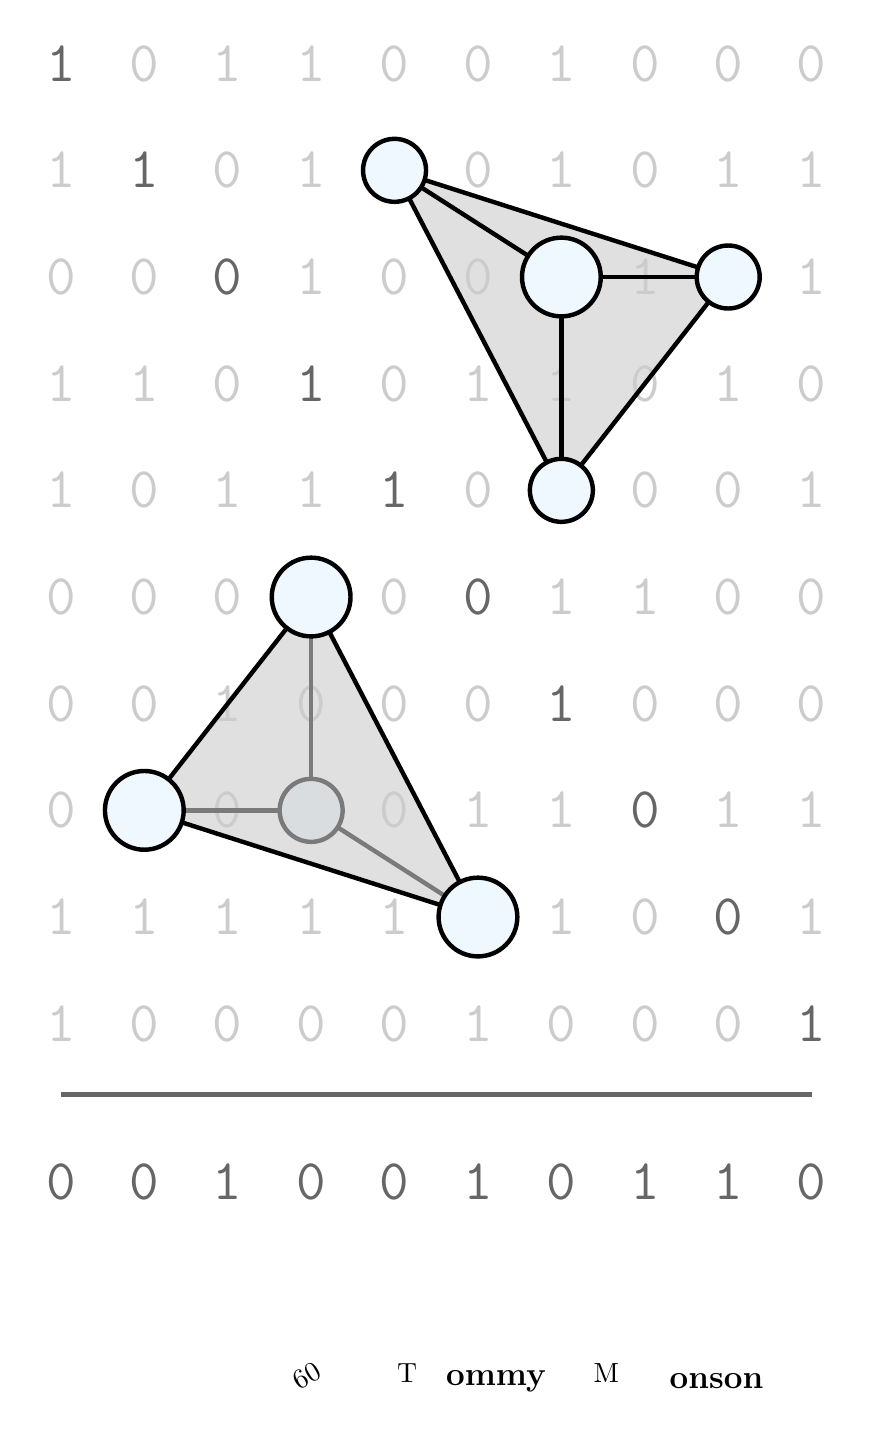
\begin{tikzpicture}
		[
		space/.style={minimum height=1.5em,matrix of nodes,row sep=6.75mm,column sep=4.5mm,style={font=\ttfamily}},
		nodes in empty cells]
				
		% Binary Matrix
		\matrix (m) [space, style={font=\ttfamily}]
		{
		\odk & \zro & \one & \one & \zro & \zro & \one & \zro & \zro & \zro \\
		\one & \odk & \zro & \one & \one & \zro & \one & \zro & \one & \one \\
		\zro & \zro & \zdk & \one & \zro & \zro & \zro & \one & \one & \one \\
		\one & \one & \zro & \odk & \zro & \one & \one & \zro & \one & \zro \\
		\one & \zro & \one & \one & \odk & \zro & \one & \zro & \zro & \one \\
		\zro & \zro & \zro & \one & \zro & \zdk & \one & \one & \zro & \zro \\
		\zro & \zro & \one & \zro & \zro & \zro & \odk & \zro & \zro & \zro \\
		\zro & \one & \zro & \zro & \zro & \one & \one & \zdk & \one & \one \\
		\one & \one & \one & \one & \one & \zro & \one & \zro & \zdk & \one \\
		\one & \zro & \zro & \zro & \zro & \one & \zro & \zro & \zro & \odk \\
		};
	
		\matrix (d) at (0,-8.1cm) [space, style={font=\ttfamily}]
		{
		\zdk & \zdk & \odk & \zdk & \zdk & \odk & \zdk & \odk & \odk & \zdk \\
		};
	
		\begin{scope}[scale=0.2]
		
			% Pyramids
			\coordinate (A) at ($(m-6-4.center)$);
			\coordinate (B) at ($(m-8-2.center)$);
			\coordinate (C) at ($(m-9-6.center)$);
			\coordinate (D) at ($(m-8-4.center)$);
			
			\draw [ultra thick] (D) -- (A);
			\draw [ultra thick] (D) -- (B);
			\draw [ultra thick] (D) -- (C);
			
			\draw [ultra thick,fill=textbook-blue] (D) circle (2);
			
			\draw [ultra thick, fill=light-gray, fill opacity=0.6]
			(A) -- (B) -- (C) -- cycle;
			
			\draw [ultra thick,fill=textbook-blue] (A) circle (2.5);
			\draw [ultra thick,fill=textbook-blue] (B) circle (2.5);
			\draw [ultra thick,fill=textbook-blue] (C) circle (2.5);
			
			%----------------------------------------
			
			\coordinate (A) at ($(m-5-7.center)$);
			\coordinate (B) at ($(m-3-9.center)$);
			\coordinate (C) at ($(m-2-5.center)$);
			\coordinate (D) at ($(m-3-7.center)$);
			
			\draw [ultra thick, fill=light-gray, fill opacity=0.6]
			(A) -- (B) -- (C) -- cycle;
			
			\draw [ultra thick] (D) -- (A);
			\draw [ultra thick] (D) -- (B);
			\draw [ultra thick] (D) -- (C);
			
			\draw [ultra thick,fill=textbook-blue] (D) circle (2.5);
			
			\draw [ultra thick,fill=textbook-blue] (A) circle (2);
			\draw [ultra thick,fill=textbook-blue] (B) circle (2);
			\draw [ultra thick,fill=textbook-blue] (C) circle (2);
			
			%----------------------------------------
			
			% Dividing Line
			\coordinate (L) at ($(m-10-1.center) + (0,-4.5cm)$);
			\coordinate (R) at ($(m-10-10.center) + (0,-4.5cm)$);
			
			\draw [ultra thick,dark-gray] (L) -- (R);
			
			% Author
			\node [rotate=30] (A) at (-8.5cm,-53cm) {\fontsize{26}{26} \adforn{60}};
			\node (B) at (-2.15cm,-52.65cm) {\fontsize{20}{20} \spacedallcaps{T}};
			\node (C) at (3.5cm,-53.165cm) {\fontsize{12}{12} \spacedallcaps{\bfseries ommy}};
			\node (D) at (10.5cm,-52.65cm) {\fontsize{20}{20} \spacedallcaps{M}};
			\node (E) at (17.5cm,-53.165cm) {\fontsize{12}{12} \spacedallcaps{\bfseries onson}};
		\end{scope}
		
		\end{tikzpicture}
	\end{center}
\end{tcolorbox}
\end{center}
\end{titlepage}

\newpage

%--------------------------------------------------------------------------------
%--------------------------------------------------------------------------------
%    TABLE OF CONTENTS
%--------------------------------------------------------------------------------
%--------------------------------------------------------------------------------

% Text length of lowercase alphabet
\newlength{\alphabet}
\settowidth{\alphabet}{\normalfont \fontsize{11pt}{11pt} abcdefghijklmnopqrstuvwxyz}

\newgeometry{top=2cm, bottom=2.5cm, textwidth=2.9\alphabet}

\setcounter{tocdepth}{3} % Set the depth of the table of contents to show sections, subsections, and subsubsections

\tableofcontents % Print the table of contents

\newpage

%--- FINAL CHECKS -----------------------

% Standard spacing before and after special content
% Adverbs. Don't use them unless they work really well.
% Header check

%--------------------------------------------------------------------------------
%--------------------------------------------------------------------------------
%    PREFACE
%--------------------------------------------------------------------------------
%--------------------------------------------------------------------------------

% Search for section references at the end of the writing process and use latex commands for them.

\part*{Preface}
\addcontentsline{toc}{section}{Preface}

\begin{displayquote}
\textit{I wrote my first novel because I wanted to read it.}
\begin{flushright}
	---Toni Morrison
\end{flushright}
\vspace{4mm}
\end{displayquote}

% I just read it. It's good. And coming from someone who is so self-critical, that's high praise.

% "I just wondered how things were put together." - Claude Shannon

% 2019 has been a strange year for me.

In December of 2018, I graduated from Duke University, feeling like I knew simultaneously very much and nothing at all.

% Why did you write this?
% Why do you think its worth sharing with others?
% Why read this over a traditional textbook?
% College gave me reasoning and knowledge. Writing this guide gave me intuition.
% When you get to the end of any extended course of study, you tend to gain *insights*. I don't understand why these insights need to be so hard-earned. Why can't there just be a textbook full of the insights?
% Categorizing things is an age old approach to philosophy and science.
% Wax poetic about computer science.
% At times, I struggled writing this book. But I eventually came to a point where I knew what this book was trying to be, and I could envision it. I could see the pieces linking together,  and I wanted it to exist. I wanted to lay out, in simple English, the connections I was making in my mind. I wanted to share these difficult concepts in a way that was accessible.
% Talk about what it was like to just live in this document for like multiple months.
% The value in spending time just philosophizing about things.
% Belief that the most significant, cutting-edge, and interesting jobs in many fields require or would benefit greatly from a deep philosophical and mathematical understanding of software.
% In the end, I was tired of being confused.
% At a certain point, I stopped worrying about what important to know for technical interviews. I was making educated decisions daily about what was essential and what was optional, what was foundational and what was derivative.
% Mechanical engineering vs. computer science. They have many similarities, and my true interests likely lie between the two.
% Sometimes writing this was a Herculean effort. Sometimes it wrote itself, and I just sat there and watched it happen.
% The physical and mental toll of writing this book.
% Was it worth it all the time and effort and isolation? I feel I have given myself a great gift. And now I would like to offer this gift to you.
% "Quasi-graduating"

% Sign just with initials T.M.?

\newpage

%--------------------------------------------------------------------------------
%--------------------------------------------------------------------------------
%    ACKNOWLEDGEMENTS
%--------------------------------------------------------------------------------
%--------------------------------------------------------------------------------

\part*{Acknowledgements}
\addcontentsline{toc}{section}{Acknowledgements}

% The process of note taking while writing this book. Deciding whether to put my thoughts into note-form, and, thus, potentially into published-form. The notes were the barrier between "that's stupid/irrelevant/misinformed/way too \textit{out there}" and "Perhaps---that might be a good idea\dots"
% But I also adhered to the principle of "If it's really that good of an idea, you'll remember it."
% I didn't write notes about the people in my personal life who deserve and have my utmost gratitude. I had my ideas, but I knew that, in the end, I would remember those who I truly want to thank, and I would remember exactly why. Some things are better thought through with the heart than with the brain.

%--- PERSONAL ---------------------------

% DA teachers
% Duke teachers
% My good friends, those few people with whom it's never been anything less than \textit{real}, honest and earnest to infinity and beyond. Interacting with you all is what makes my world go 'round.
% Parents

% In addition, I also have a number of professional and academic people (and works) to acknowledge.

%--- PROFESSIONAL AND ACADEMIC ----------

% Dan McPherson, his analytical mind and precision
% TeX, TeXStudio, Donald Knuth
% Robert C. Martin and his book \textit{Clean Code}, which I referenced occassionally for the purpose of book design. Like the book you are reading now, Clean Code presents material that is typically considered rather dry and \textit{compels} you to care about it. It accomplishes this largely due to its writing style and short sections. It isn't afraid to be whimsical after a dense section, and it has many section headers (sometimes more than one per page), which act as \textit{mini-checkpoints} for the reader. I studied the narrative structure of Clean Code and applied many of its stylistic and typographical principles to the typesetting of this book.

%--- ECCENTRIC --------------------------

% And, last but not least, I have a number of somewhat eccentric thank-yous to give. Despite how unconventional some of these shoutouts are, they are nevertheless sincere.

% Seinfeld (Theory of Comedy, comedy systems, categories of comedic timing)
% DGR, Fantano
% Morinaga & Company, Ltd., the producers of Hi-Chews

\newpage

%--------------------------------------------------------------------------------
%--------------------------------------------------------------------------------
%    OPENING QUOTE
%--------------------------------------------------------------------------------
%--------------------------------------------------------------------------------

\vspace*{4cm}
\begin{center}
\textit{The very word intuition has to be understood. \\[5mm]
	You know the word tuition---tuition comes from outside, somebody teaches you, the tutor. \\[5mm]
	Intuition means something that arises within your being; \\[5mm]
	it is your potential, that’s why it is called intuition. \\[5mm]
	Wisdom is never borrowed, and that which is borrowed is never wisdom. \\[5mm]
	Unless you have your own wisdom, your own vision, \\[5mm]
	your own clarity, your own eyes to see, \\[5mm]
	you will not be able to understand the mystery of existence.}
\begin{flushright}
	---Osho
\end{flushright}
\end{center}

\newpage

%--------------------------------------------------------------------------------
%--------------------------------------------------------------------------------
%    BODY CONTENT
%--------------------------------------------------------------------------------
%--------------------------------------------------------------------------------

%--------------------------------------------------------------------------------
%--------------------------------------------------------------------------------
%    CHAPTER 0: INTRODUCTION
%--------------------------------------------------------------------------------
%--------------------------------------------------------------------------------

% Simple art above each chapter title? Like 10mm tall and \textwidth across?

\part*{Introduction}
\addcontentsline{toc}{part}{\tocpartglyph Introduction}

% “When I use a word, it means just what I choose it to mean — neither more nor less.” - Alice in Wonderland

\begin{displayquote}
\textit{What is this thing that flickers past my gaze? \\
	No more, no less than what my mind hath wrought.}
\vspace{4mm}
\end{displayquote}

I find it difficult to describe what this book is. And yet, I find it easy to express why I think it is worth your time and contemplation.

% https://www.standoutbooks.com/nail-non-fiction-introduction/

% The hook starts here. Why should the reader care?
% Five reasons to read this book: 1. It is a work of passion, born out of a consuming and frenetic obsession, a labor of love; 2. It is painstakingly crafted, like a sculpture hewn from granite, every sentence carefully constructed, every word meticulously chosen; 3. It is a work written in the midst of a deep depression, and it serves as a guide to those who may experience the same feelings of self-doubt; 4. It is a distillation of some very difficult and important ideas that you have encountered and will undoubtedly encounter again; 5. It's short and tries not to waste your time...
% However, there is a reason that is bigger than all of these...

% The computer is the most important invention since the printing press. It is a game changer for mankind. The amount of science being done now is enormous compared to what was being done in, for example, Newton's time. Back then, there were very few scientists, and they used simple tools. The body of human knowledge started kicking into gear at the turn of the 20th century, and it took off like a rocket with the conceptualization and implementation of general-purpose computers. Before we did a few calculations a minute on a slide rule. Now, consumer CPUs can do \textit{billions of calculations per second} and supercomputers are well into the territory of \textit{quadrillions}. Human life has been immensely altered by computers.
% Computers are everywhere today. They are essential to modern life, and they will only become more essential. Thus, they are worth understanding.
% Computers are complicated, but they are built on simpler principles that were discovered incrementally as humanity gained knowledge. To someone who is ignorant of these earlier ideas, computers look like magic. Some programmers think that computers are magic, and yet they can still program, thanks to software abstraction. However, you will reach a conceptual limit if you rely on abstractions.
% As technology gets more complicated, it gets harder to understand it without this intuitive, foundational knowledge. If you see yourself utilizing computers frequently for the remainder of your life, the time to learn about them is now.
% The book gets more programming-oriented as it goes on. I am hoping that the book as a whole is compelling enough that you will not notice it. Even if programming does not interest you, the theoretical parts of the book will teach you how things work and the application parts will teach you how to make great things. If you are not interested in that, you should be.

% What is this thing? A book? A textbook? A work of non-fiction? A list? A guide? A handbook? I think it is all of those things.

% It's a book about programming, and a guide for software engineering interviews, but it's more than that. I think it will be interesting and useful for anyone who wants to create and analyze things effectively.

% Technically, a book is a physical medium that acts as the vessel for a \textit{text}, a written work, a determinate sequence of abstract symbols. Thus, I will refer to this work hencefore as a text.
% What is the computer equivalent of a text? A text file, an abstract sequence of numbers. Do computer files exist? They manifest in physical reality as voltage levels, yes. However, the recognition of these voltages as elements of a pattern is conceptual. This is the case for all patterns, for all things more complex than singular, indivisible objects. So the abstract, informational content of a story does not exist in physical reality, but a computer can contain an electrical phenomenon within its memory that can be interpreted as the content, given the appropriate algorithm.

%----------------------------------------

% Use short paragraphs. Be concise. Make it conversational.
% Make it inspiring. Make it motivational. Make it sound accessible.
% A subsection called administrivia for book-structure information.

% Discuss the goal of this guide. Discuss why someone might want to read it.
% Discuss why content was chosen and why it is ordered the way it is.
% Discuss why certain topics were left out.
% Give a section by section overview. Raise some of the central questions.
% Give a warning for the Theory of Computation section lol. Or at least assure readers that things will become more applied as the guide progresses.
% Discuss the title. Intuition. Definitions in my own words - "if you know something's name, you have power over it." True name, mysticism.
% Make your own guide!

%--- METHODOLOGY ------------------------

% I begin writing this so that understand it. Then, it got big enough that I thought it could be of use to others, so I started to write it in such a way that someone with less formal education than me could understand it. Then, I realized that in order to really get it, I had to write about these complex topics in such a way that someone outside of CS could feasibly understand it, given enough time and drive. I wanted to explain the insights one can glean from higher mathematics and theoretical computer science, and I wanted to do it in such a way that it was really easy to understand. This is intuitive understanding. Semantic understanding. In hacker terms, to grok something.
% The words on the page will not teach the material to you. They are simply there to guide your thoughts toward understanding. You have to spend time in thought to foster intuition.
% You might find the tone of the book to be conversational. This is because I don't know how to teach in any way besides conversation.
% More information does not mean more understanding. File sizes denote information - movies vs. books.
% This guide began as a study list for software interviews. What does it mean to study for a software interview? Is it just doing a bunch of sample problems? How prepared should you be? Is the goal simply to receive an offer or to be a truly excellent candidate? I would argue that it is better to pursue the latter, if possible, because it means you are building yourself, not just building a temporary performance that will be showcased at interviews. You make yourself an asset. Also, as long as you have only a surface-level understanding, you will always feel like a fraud who knowledge is fragile and constantly waning.
% The question should not be "How do I get a competitive software engineering job?" It should instead be "What makes a truly excellent software engineer?"
% While jargon is confusing to people who are not 'in the know', it is usually very descriptive. It paints a very precise picture, if you know how to differentiate similar terms. The English words that are used are often quite apt. Differentiation and integration as examples.
% There are a lot of jargon terms in computer science, and a lot of them are very similar. This guide also serves as a personal dictionary of sorts.
% This book champions a semantic approach to the content covered. I personally cannot be satisfied with only equations and hand-waving explanations for what they represent. This does not mean that it focuses on applied math rather than pure math. On the contrary, there is a fair amount of pure math here. However, good teachers tend to plot pure mathematical structures and explain them with metaphors to make them familiar. The philosophy here is that in order to learn something new, you must be able to compare it to something you already understand. If a non-trivial topic is 100% foreign to you, you can't learn it, no matter how hard you try.
% This book is written in a poetic/oratory style. It flows like a speech that is meant to be read aloud. I encourage you to do so.
% The book is slanted toward imperative programming, specifically toward OOP. This is because most software engineering is done in OOP languages. OOP is also less abstract and thus more beginner-friendly. Declarative programming and functional languages are discussed with a decent level of detail, but OOP is the default here. For example, the implementation chapter explores Java.

% What makes this book different from most textboooks is that it starts from first principles.
% The first two sections are top-down. Once we understand information, communication, and logic, the rest of the book is bottom-up. And then software engineering might be top-down again.
% Bottom-up is like starting from an arche, top-down is like starting from henosis.

% Why do people think they can't do math? What is so confusing about it to them? I collected some responses, thought about it, and tried to make this text as accessible as possible for those people.

% Blue boxes are tangential material and out-there concepts
% Make a chart with philosophy as a circle (a non-metric space) and mathematics, physics, engineering, computer science, etc. as bars (metrics spaces whose metric is academic complexity). The bars start at high-school level topics and extend to the bleeding edge of understanding. Draw two versions: what college taught me vs. what I felt like I needed to know. Syntactic understanding vs semantic understanding.
% College dug deep, raw tunnels into hard earth. <Drawing of vertical lines>. Writing this book connected them all horizontally, leaving lanterns at the intersections so that one could see all the way from one end to the other. <Drawing of criss-crossing lines and nodes>. Now, picture these tunnels instead as interlocking length of fishing line. With my net woven, I can catch fish instead of floundering in the water with loose strings.

% Computer science is not about computers, it is about computation. Computation is much broader than the study of computers. The concepts are everywhere.
% Comment on these CS etymology alternatives: turingineer, turologist, datalogy, flow-charts-man (hilarious), applied metamathematician, applied epistemologist, hypologist (study of what is under? as in under systems?), computics (like 'physics', the science of computational phenomena, great name), computing science (equivalent to computics, but not Greek and not as cool) automatic information (pertaining to automata), infomatics ("what can be conceived," pretty badass, similar to mathematics ("what can be learned"), unfortunately taken).
% What about the phrase "theoretical computer science"? The better term is computational science.
% Not CS: information science (more associated with effective storage and dissemination of information, not computation), information technology (a business-oriented discipline focused on choosing and maintaining hardware and software for a company), software engineering (the effective implementation of theoretical CS concepts for the purpose of building software)
% "I will rate these names based on accuracy, but I won't deny my bias toward the coolest sounding names"

% Chapters and sections.

% Interdisciplinary, historical approach.
% There are a lot of quotes. I like quotes. Plus, taking a bunch of quotes out of context (slashthrough) \textit{repurposing} quotes allows me to pretend like a bunch of smart people agree with what I am saying. And they all write a part of my book for free. Ha, suckers!
% I remember the death quotes in Call of Duty 4 (quite profound in their context, especially considering it's Call of Duty). Quotes can sound profound even when you are not mature enough to really understand them (like quotes about war). "War is delightful to those who have not yet experienced it." - Erasmus. "My first wish is to see this plague of mankind, war, banished from the earth." - George Washington (and then America goes on to be in almost constant war).
% Good quotes succinctly capture the essence of a hard-to-know truth. Mathematical formulas are basically quotes.
% This material is "advanced," but it is not inherently hard. If you perceive any material as hard, here or elsewhere, that either means that you are unfamiliar with it and you need to muse on it for a while (perhaps by covering more elementary topics first) or that it is being taught poorly.
% I'm not a PhD. Most people who write textbooks are. This is still a textbook. It is meant to be educational.
% I am not very old. Most people who write textbooks are older. (I learned much of this material as I was writing it. Most people who write textbooks know the material beforehand.) However, I think this is a benefit in some sense because I am not so far removed from my readers.
% People should catalog their knowledge in a professional format. We spend so much time and effort learning, and then we just accept that we will forget the vast majority of it. I remember cramming for my linear algebra final (a class I had no business taking in my first semester of college). A few hours before the test, I drawing some matrices on a whiteboard and I thought that that point in time would likely be the best that I would ever understand linear algebra. Beyond that point, my understanding would slow die. And I thought that was very sad. I also read that many software engineers forget most of what they learned about CS. That's also sad.
% Italics are used to mark emphasis, but the kind of emphasis marked depends on context. Sometimes, an italicized word is a \textit{keyword}, which means that it is a technical term and that I want you pause for a half-second to absorb its meaning. Other times, the italics merely denote a \textit{vocal cue}. Words from languages other than English are also italicized.
% Content is presented in a culturally neutral way and does not assume a great deal of prior knowledge.
% The book tries to get the point across that there is more than one way to think about things and that knowledge is built on assumptions, including the body of knowledge called computer science. While we must work within a box, we should strive to remind ourselves periodically that we are, indeed, in a box and that there exist methods of thinking outside of it. The theories and models we use today may simply be the predecessors of theories and models to come. The topics of discussion, however, are eternal.
% Traditional education is bottom-up (notice how stuff on Earth falls when it's dropped => that's because this law F_g=ma_g exists). This book uses a top-down approach (in the abstract sense, what is mass, acceleration, force, objects, motion, distance, space => given all of those ideas, we observe that F_g=ma_g happens in this Universe). The traditional approach is syntactic, this book's approach is semantic. The "top" in this case is philosophical and mathematical theory: large-scale ideas, objects, and relations. We spend a substantial amount of time talking about these huge, fundamental concepts and how they appear in philosophy, logic, mathematics, physics, linguistics, etc. Once this information theory is built, we use our newfound mathematical insight to model computation and computational phenomena (automata, DS&A, programs). In doing so, we develop a theory of computer science. We then use this theory to understand principles of software engineering.
% The abbreviations i.e. and e.g. are used frequently in this book. What do those mean?
% If there's a word you don't know, just look up the definition and keep going. That's basically how I wrote this book.
% There are times when I speak very precisely and times where I am more casual. I believe it will be easy to tell which mode I am in from context. If you see a lot of italicized keywords and dense sentences, that probably means I am speaking precisely. If you see poetic language, absolute statements, or contractions, that probably means I am speaking casually.
% This document uses A4 paper size. Print it out and put some staples in it if you would like a hard copy. If you are a US Letter-using heathen, there is also a US Letter version available for your convenience. (And in the US Letter version, write something else).
% You may be interested in seeing the LaTeX code that I wrote to compile this book. You can find it at ...

% Looking at a bird he says, 'Do you know what that bird is? It's a brown throated thrush, but in Portuguese, it's a... in Italian, a...' he says "in Chinese, it's a... in Japanese, a...,' et cetera. 'Now,' he says, 'you'll know absolutely nothing whatsoever about the bird. You only know about humans in different places and what they call the bird. Now,' he says, 'let's look at the bird." - Richard Feynman (recalling his father, The Pleasure of Finding Things Out)

% "So many people today---and even professional scientists---seem to me like somebody who has seen thousands of trees but has never seen a forest. A knowledge of the historic and philosophical background gives that kind of independence from prejudices of his generation from which most scientists are suffering. This independence created by philosophical insight is---in my opinion---the mark of distinction between a mere artisan or specialist and a real seeker after truth." - Albert Einstein

% Suppose your goal is to be a great musician. You can either fool around with the tool enough until you glean a sense of what works and what doesn't (play guitar, pick up music theory along the way) or you can learn the theory and use it to understand the tool fully (learn music theory, apply it to whatever instrument you want). You'll be making music faster the first way, but it will always be sort of mediocre and you'll hit a knowledge ceiling. With the second way, you will have an in-depth understanding of how music works and now all you need is implementation (learn an instrument, produce digital music, get other people to play your work).
 % Introduction
%--------------------------------------------------------------------------------
%--------------------------------------------------------------------------------
%    CHAPTER I: COMPUTATION
%--------------------------------------------------------------------------------
%--------------------------------------------------------------------------------

\part*{Philosophy of Computation}
\addcontentsline{toc}{part}{\tocpartglyph Philosophy of Computation}

\vspace{4mm}
\begin{displayquote}
	\textit{We're presently in the midst of a third intellectual revolution. The first came with Newton: the planets obey physical laws. The second came with Darwin: biology obeys genetic laws. In today’s third revolution, we're coming to realize that even minds and societies emerge from interacting laws that can be regarded as computations. \textbf{Everything is a computation.}}
	\vspace{2mm}
	\begin{flushright}
		---Rudy Rucker
	\end{flushright}
\end{displayquote}
\vspace{4mm}

\textit{Computation} is an essential part of being human. Just as we act on our perceptions, feel our emotions, and daydream in our imaginations, we also compute with our \textit{reasoning} in order to find answers to the questions we have about life. \\

One can describe computation in a variety of ways. Some are poetic, others are more formal, and many we will discuss at length. In doing so, we will generally flow from poetry to formality, starting with broad statements and colorful examples and progressing toward a formal understanding. For now, we will say that computation is a process which resolves \textit{uncertainty}. \\

In his \textit{Theogony}, the Ancient Greek poet Hesiod (fl. 750 BCE) depicts a fascinating uncertainty called Chaos: a vast nothingness that preceded the creation of the Universe. From this void emerged the primordial deities, personifications of nature who gave life to the Titans and, by extension, to the Olympian gods. Curiously, the modern definition of \textit{chaos} has nearly inverted. Now, one might say that a situation is \textit{chaotic} if there is \textit{too much} going on. Despite their great conceptual difference, these meanings share a common property: they both evoke \textit{confusion}. \\

This place in which we find ourselves may indeed be post-Chaos, but confusion remains a familiar state for us. In fact, it is our natural state. We come into life confused about everything---crying, open-eyed in reaction to how much is going on around us. Slowly, we figure a few things out. Later, we consider many things \textit{certain}. As time ticks on and we carve our separate paths in the world, the wise ones among us come to realize the true depth of their confusion. \\

Although we are initially confused, we naturally pursue an understanding of the chaos that surrounds us. We perceive the goings-on of our environment and organize them into patterns that orient us and give meaning to the disorder of our existence. This is the crux of computation. It is the structured manipulation of \textit{data} into \textit{information} for the purpose of acquiring \textit{knowledge}. It shines a light into the darkness we call home. \\

These terms---data, information, and knowledge---are broad enough to apply to a variety of systems. In fact, they appear in nearly every academic field and certainly within those that strive for objectivity. One can have data on, information about, and knowledge of anything that can be observed or experienced. As such, it is difficult to confine these terms to short and tidy definitions that are both rigorous and free of controversy. We will have to settle then for a long, pragmatic discussion. \\

Still, we must start somewhere. For example, you already have an idea of what information is, and it is likely that your intuition is broadly correct: information is a thing that tells you something. As we dive into more and more abstract topics, do not hesitate to, in this way, fall back on your existing vocabulary for support. A word used technically is more precise than the same word used casually, but the gist of it all is often the same. Or there is at least some sense in which they mirror each other. \\

Recall the usual context in which technical language is born. A phenomenon is observed by a community, and it becomes the subject of casual discourse. It may even be a widespread concept that is discussed by society at large, in some way or another. The phenomenon is accordingly given an \textit{informal definition} and a name (or, perhaps, many names). Interested theoreticians then study the structure of the phenomenon and \textit{formalize} it. They give it a \textit{formal definition} and bestow it a more permanent name, either one used previously or something new that is, in the namers' opinion, more apt. In the latter case, the new term is disseminated throughout the community and perhaps to the wider public, where it may either replace or coexist with previous informal terms. \\

Regardless, the namers must reach outside of the formalisms they have constructed and find a word from an informal language that captures the essence of their abstract thought. This is the beauty of good jargon: such a word will, to an amateur, shed a shallow but wide light into the vast space of an idea, but it will also illuminate the whole shebang in the eyes of an expert, evoking in its concise informality all that he or she has previously learned on the subject. \\

In the spirit of this principle, our three words are defined softly below to act now as beacons in the dark of our ignorance and later as shining summaries of our hard-earned understanding: \\

\begin{displayquote}
	\textbf{Data} (sing. \textbf{datum}) are pieces of information that are meaningless when considered separately. They are observable lacks of uniformity in reality, each of which may be represented by a symbol that conveys its particular difference from the norm. \\~\\
	\textbf{Information} is an ordered arrangement of data that is considered meaningful. The data are arranged such that the information as a whole complies with the grammar of a language that can, in theory, be understood. \\~\\
	\textbf{Knowledge} is an understanding of information that emerges given proper interpretation and sufficient thought. It is usually associated with Truth and may be considered a body of true beliefs. \\
\end{displayquote}

The journey toward an honest comprehension of these terms will be an arduous one, requiring an open mind and an ample store of time set aside for contemplation. And in walking the path, you may find that it meanders or veers off suddenly, that what you desire remains frustratingly out of reach or nowhere to be seen. But as the text winds its way through the domains of psychology, cognitive science, philosophy, physics, information science, linguistics, logic, and mathematics, remember to lift your eyes up from the page and to mull over the ground you have covered so far. The essence of computation is found at the crossroads of these disciplines, and a fuller appreciation awaits at each passing overlook. \\

There is a fourth word---\textit{wisdom}---but we leave it undefined for now. Nevertheless, its importance cannot be overstated. \\

% The wisdom can be found in the characters.
% Game metaphor, good players

%----------------------------------------

In this chapter, we will explore what computation is and why it matters. Computation is a kind of game in which \textit{pieces} are moved and transformed within a \textit{game space} according to a predetermined set of \textit{rules}. However, unlike most games, computation has no set goal. Nature shuffles its hazy pieces about, following arbitrary rules for reasons we cannot ascertain. Man, on the other hand, explicitly defines its pieces and rules, modeling them after Nature's strange mechanics. We declare the win conditions of our problems and play toward them, hoping that our computations will elucidate the knowledge we seek. \\

\begin{description}
	\item[Section 1:] \textit{Cognition and Consciousness}
	\item[Section 2:] \textit{Natural Philosophy and Physics}
	\item[Section 3:] \textit{Information and Communication}
	\item[Section 4:] \textit{Logic and Mathematics} \\
\end{description}

Here, we learn how this game is played and how it is woven into the fabric of our reality. In the chapter following this one, we model the game of computation mathematically and find the theoretical limits of what it can tell us. Beyond that, we learn how to be an excellent player, covering \textit{techniques} for efficient problem solving and \textit{tools} for designing beautiful, maintainable systems. \\

%----------------------------------------

With that said, let us take a page from Hesiod and begin our tale with an uncertain chaos. Let us regard reality as a baby might: confusing but ultimately intelligible through \textit{categorization}. \\

%--------------------------------------------------------------------------------
%    SECTION: COGNITION
%--------------------------------------------------------------------------------

\toclineskip
\section{Cognition and Consciousness}

\vspace{4mm}
\begin{displayquote}
	\textit{If you wish to make an apple pie from scratch, you must first invent the universe.}
	\vspace{2mm}
	\begin{flushright}
		---Carl Sagan
	\end{flushright}
\end{displayquote}
\vspace{4mm}

Dark turns into light. A boundless zephyr of blurs. You see. You hear. You \textit{feel}. The knife-edge of experience materializes, and you step out onto it. It cuts you, and there is no thought---only sensation. Air kissing skin and turbulent color. Sonic frenzy and the feeling of self-weight. Reality emerges raw and beams through all you are. You are lost in it all: a sailboat in a storm, a satellite adrift in space, and the rest. Indifferent, the phantasmagoria rages on. \\

% Thing
% Individual, Attribute, Class, Relation

% Everything
% Universe
% Domain of discourse
% Context/POV

% Physical
% Perceptual
% Conceptual

% Dichotomy (partition, differentiation, cut): pt()
% Attributes (properties)
	% Quality vs. Quantity
	% Magnitude vs. Multitude
% Something
% Negation
% Nothing

% Collection (unification, integration): ref(...) or {...}
% Classes (sets)
% Extension
% Intension
% Well-foundedness

% Transitivity (Parthood vs Membership)

% Reference
	% Referential universe is isomorphic to referent universe
		% Extrinsic iso: both universes, part of nothing else
		% Intrinsic iso: both atoms, partless
% Perception
	% Meronomy, parthood
	% Attention
% Conception
	% Taxonomy, subset, is-a
% Naming (inverse: recognizing, understanding)
	% Copula (is-a)
% Communication

% Dimension
	% Nominal (trivial)
	% Order (hierarchy)
		% Referential order
		% Conceptual order
	% Metric
% Atom
% Space and time
% Modality
% Trivial dimensions

% Causality

% Identity: spatial, temporal, referential, isomorphic
% Individuation (self/other) (functionally equal to dichotomy)
% Analogical reasoning => isomorphism

% Map-territory relation

% Closed world
% Open world

% Contiguity
% Continuity

% Sentence
% Noun, adjective, verb, adverb
% Gerund
% Binary tree form: noun phrase + verb phrase
	% Dynamically-constructed concept
% Ternary form: concept, copula, definition
% Verb tense
% Verb transitivity affects dimensionality

% Mereology vs. Set Theory
% Function composition vs. set intersection
% Functional vs. OOP?

% Bootstrapping
% Analog magnitude representation (cardinality)
% Parallel individuation (up to 3)
% Serial ordering
% => Children induce the successor function

This is roughly the experience of a newborn infant. For children of a month or so, life is a sensory mayhem of little sense. They are not conscious, at least not in the way that we typically think of consciousness. They are, however, aware of their surroundings and sensitive to \textit{phenomena} (i.e. the \textit{appearances} of reality, \textit{observables}). To newborns, the world is not a system of distinct parts but an all-encompassing soup of stimuli. Their sensory organs input data that they do not understand, and they then output \textit{reflexes} honed through millions of years of natural selection. \\

This is not to say that babies are mindless. Rather, their minds are just unlike those of typical adults, which both \textit{filter} and \textit{store} information. For example, while babies and adults have similar hearing ability, babies nevertheless hear things that adults do not. This is because adults subconsciously ignore certain sounds; they may \textit{sense} the auditory data, but they do not \textit{perceive} them. This filtering process is called \textit{sensory gating}, and it inhibits any stimulus that is deemed irrelevant. Any information that is not filtered is then eligible for storage in \textit{memory}. \\

Thus, if the adult mind is like the conical beam of a flashlight, seeing far but neglecting much, the baby mind is like the radiant orb of a lantern, seeing everything nearby but illuminating nothing deeper. These configurations are well-suited to the goals of each: the adult needs \textit{attention} to understand complex situations whereas the baby needs \textit{unrestricted perception} to acquire as much information as possible. Unburdened by categorical thought and sensory gating, babies live in the present and see the \textit{suchness} of reality. However, their experience is not quite the \textit{kensh\=o} of Zen---it is more like Aldous Huxley's Mind at Large or William Blake's metaphor, from which Huxley took the title of his first essay on psychonautics: \\

\begin{displayquote}
	If the doors of perception were cleansed every thing would appear to man as it is: Infinite. For man has closed himself up, till he sees all things thro' narrow chinks of his cavern. \\
\end{displayquote}

So it is through a great deal of concurrent filtering and learning that we come to build a cavern around ourselves. But we do not muffle our perception pointlessly---we trade it for genuine \textit{thought}. \\

\subsubsection{Percepts and Concepts}

There is a distinction that is sometimes made in cognitive science between a \textit{(phenomenal) P-consciousness} and an \textit{(access) A-consciousness}, the former being the sole consciousness of the baby mind, concerned only with bits of immediate, subjective experience known as \textit{qualia} (e.g. what it is like to \textit{feel} a delicate raspberry as it touches your tongue, what it is like to \textit{taste} it as you mash it between your molars, the rush of brief and unique \textit{delight} found in enjoying that \textit{particular} berry, etc.) and the latter being the dominant consciousness of the adult mind, concerned with \textit{cognitive information} (e.g. thoughts about sensory data, abstract ideas, memories of the past, plans for the future, and all things involved in \textit{mental computation}). \\

Of course, adults still have a P-consciousness---we can lose ourselves in the moment if we are willing. But ours is a boarded-up P-consciousness, largely unaware of the immense volume of all that is happening at all times. Perhaps it is only the bodhisattvas or the mystics of yore who truly come to know their infant minds again and see the P and A as they are: two \textit{modes} of a unified whole. Or perhaps, more pessimistically (and as Huxley suggests), the P in its unadulterated totality is really a kind of schizophrenic insanity, and it is only by the grace of our specialized neural hardware that we erect defenses against its sensory onslaught. Alas, the suchness of such a consciousness eludes those of us with at least one foot planted solidly on the earth. \\\\

\begin{tcolorbox}[breakable, enhanced, colback=textbook-blue, sharp corners]
	\vspace{3mm}
	\begin{center}
		\textbf{The Hard Problem of Consciousness}
	\end{center}
	What is it about phenomenal consciousness that is so intangible? It has been a question of interest to humanity for thousands of years and an object of formal study since Ren\'e Descartes (1596-1650) first posited the duality of \textit{mind} and \textit{body}. Inspired by the proliferation of \textit{automata} (i.e. self-operating machines) in Paris, Descartes came to suggest the extraordinary: that animals---their limbs, organs, and mannerisms---could be replicated with sufficiently complex machinery. Further, he professed that animals \textit{themselves} were machines, with bone and flesh standing in for wood and metal: \\
	
	\begin{displayquote}
		It seems reasonable since art copies nature, and men can make various automata which move without thought, that nature should produce its own automata much more splendid than the artificial ones. These natural automata are the animals. \\
	\end{displayquote}
	
	Note that Descartes implies here that animals are "without thought." He also claimed that thoughts required a language in which rational ideas could be expressed. (Thoughts encoded in a language, however, need not be expressed outwardly; babies, for example, mentally represent ideas before learning how to render them in speech.) He also reasoned on this basis that an automaton would never be able to think because it would never be able to speak in the way that humans do---by organically producing an appropriate response to any given prompt. (Whether or not he was correct remains to be seen, though the possibility of an \textit{artificial general intelligence} does not seem quite as absurd now as it must have seemed back then.) In Descartes' view, humans are special and cannot be reduced to machinery because, unlike animals, they possess rational minds enriched with a free will that no algorithm can replicate. \\
	
	Thus, Descartes championed \textit{substance dualism} (also known as \textit{Cartesian dualism}), in which all things were either fundamentally of \textit{matter (res extensa)} or of immaterial \textit{mind (res cogitans)}. He saw the human being as a union of the two disparate substances but struggled to reconcile his strict dualist views with the decidedly hybrid and experiential character of his own bodily sensations and emotions. In the sixth and final meditation of his \textit{Meditations on First Philosophy}, Descartes states that in being skeptical of his fallible senses, he understands himself to be essentially a mind, a purely thinking thing of no physical extent that is intuitively indivisible. And yet, he nevertheless \textit{feels} the qualia of his body and thus must straddle his own \textit{mind-body duality}, being, in a phrase, both flesh and not: \\
	
	\begin{displayquote}
		There is nothing which this nature teaches me more expressly [nor more sensibly] than that I have a body which is adversely affected when I feel pain, which has need of food or drink when I experience the feelings of hunger and thirst, and so on; nor can I doubt there being some truth in all this. \\
		
		Nature also teaches me by these sensations of pain, hunger, thirst, etc., that I am not only lodged in my body as a pilot in a vessel, but that I am very closely united to it, and so to speak so intermingled with it that I seem to compose with it one whole. For if that were not the case, when my body is hurt, I, who am merely a thinking thing, should not feel pain, for I should perceive this wound by the understanding only, just as the sailor perceives by sight when something is damaged in his vessel; and when my body has need of drink or food, I should clearly understand the fact without being warned of it by confused feelings of hunger and thirst. For all these sensations of hunger, thirst, pain, etc. are in truth none other than certain confused modes of thought which are produced by the union and apparent intermingling of mind and body. \\
	\end{displayquote}
	
	Fast-forward to the turn of the $20^\textit{th}$ century and general confidence in the scientific method had annealed Descartes' mechanistic philosophy into full-blown metaphysical naturalism. The Modernist movement was in full swing, quantum mechanics was being formulated, mathematics was being axiomatized, and about thirty years later the greatest minds of the era would contribute to a general theory of computation. And in the 1950s, the \textit{cognitive revolution} began, and people started to think of the mind as a complex system that could be explained in terms of information and computation. It seemed like the next logical step in human progress. Like matter had been reduced to elementary particles, like water had been reduced to H$_2$O, like genes had been reduced to DNA, so too would the mind be reduced to its constituent parts. \\
	
	And yet, there is also that deep feeling in us that the mind is something else. We are inclined to believe that there is something about consciousness that is incomparable to, say, a Rube Goldberg machine or a computer running a program, no matter how complex either may be. Namely, we feel that there is \textit{something that it is like to experience being}. In 1974, philosopher of mind Thomas Nagel (\textit{b.} 1937) brought this idea to the attention of the burgeoning field of \textit{cognitive science} with his paper \textit{What Is It Like to Be a Bat?}, in which he states that no physicalist theory will capture the essence of the mind until we come to understand its subjective aspects: \\
	
	\begin{displayquote}
		The fact that an organism has conscious experience at all means, basically, that there is something it is like to be that organism. There may be further implications about the form of the experience; there may even (though I doubt it) be implications about the behavior of the organism. But fundamentally an organism has conscious mental states if and only if there is something that it is like to \textit{be} that organism---something it is like \textit{for} the organism. We may call this the subjective character of experience. \\
	\end{displayquote}
	
	This "subjective character of experience" presents a major challenge to the belief that neuroscience will eventually reduce consciousness to a theory. The \textit{philosophy of mind} is then, perhaps, brazenly Postmodernist---inherently subjective and relativistic, with answers that will remain unknown to mankind in spite of its scientific progress. Nagel posits, for example, that we cannot conceive of the subjective experience of a bat because it is totally alien to our own experience. And further, he argues that it does no good to ground such an experience in greater and greater \textit{objectivity} (i.e. independence from human bias), that such first-person character is stripped away in the third-person framework of science: \\
	
	\begin{displayquote}
		It will not help to try to imagine that one has webbing on one's arms, which enables one to fly around at dusk and dawn catching insects in one's mouth; that one has very poor vision, and perceives the surrounding world by a system of reflected high-frequency sound signals; and that one spends the day hanging upside down by one's feet in an attic. In so far as I can imagine this (which is not very far), it tells me only what it would be like for \textit{me} to behave as a bat behaves. But that is not the question. I want to know what it is like for a \textit{bat} to be a bat.
		\begin{center}
			\mydots
		\end{center}
		If the subjective character of experience is fully comprehensible only from one point of view, then any shift to greater objectivity---that is, less attachment to a specific viewpoint---does not take us nearer to the real nature of the phenomenon: it takes us farther away from it. \\
	\end{displayquote}
	
	For Nagel, this is not necessarily a death knell for any formal understanding of consciousness, but it \textit{is} a declaration of doubt in the capacity of science \textit{as we currently know it} to shed light on such matters. His qualms lie not with physicalism itself---that is, not with the assertion that mental states are fundamentally physical---but with an overconfidence that tends to come with the territory of such a mindset. His goal is to elucidate a problem: that, while it is reasonable to believe that one's mind is the result of solely the neurobiological mechanisms in one's body, it is nevertheless \textit{unreasonable}, if we accept that qualia exist and are essential to our experience, to claim that science is presently capable of capturing the subjective character of the conscious mind within its objective bounds. \\
	
	In light of this issue, Nagel concludes with a call for the formulation of an "objective phenomenology," a framework in which qualia could be described independently of their experiencer's point of view. Only then could our subjective character of experience, which is so central to our conception of being human, be expressed "in a form comprehensible to beings incapable of having those experiences." As it stands, we cannot describe our seeing of red without analogy to previous experiences of seeing red, and in such terms we can only convey our meaning to those with eyes and brains like our own. And if bats could talk, they would be similarly unable to communicate their echolocational qualia to our sonar-ignorant minds. Thus, \textit{What Is It Like to Be a Bat?} is not a position piece on the nature of qualia but a declaration of agnosticism toward it: we cannot say anything objective about what we feel until we determine whether or not our feelings have objective content. \\
	
	Nevertheless, Nagel is often considered a standard-bearer for \textit{property dualism}, which holds that there are two distinct kinds of properties: \textit{physical} and \textit{mental}. Unlike Cartesian dualism, this position holds that there is only one kind of substance, and, in contemporary Western philosophy, it is almost always considered physical rather than mental, an objective entity rather than a subjective one. But Nagel is particularly a standard-bearer for a variety of property dualism known as \textit{neutral monism}, which offers a middle path: that everything is composed of a neutral stuff that is neither physical nor mental. An early form of this view was put forth by the pragmatic philosopher William James (1842-1910) in his essay \textit{Does Consciousness Exist?}: \\
	
	\begin{displayquote}
		My thesis is that if we start with the supposition that there is only one primal stuff or material in the world, a stuff of which everything is composed, and if we call that stuff 'pure experience,' the knowing can easily be explained as a particular sort of relation towards one another into which portions of pure experience may enter. The relation itself is a part of pure experience; one of its 'terms' becomes the subject or bearer of the knowledge, the knower, the other becomes the object known. \\
	\end{displayquote}
	
	So there is a particular relation $\rightarrow$, one among many, and it is called \textit{knowing}. And it relates one term $A$ to another term $B$. And we say that $A$, the knower, \textit{knows} $B$, the known: $A \rightarrow B$. And all of these---the $\rightarrow$, the $A$, the $B$, and the composed whole---are of a neutral, experiential substance. And, indeed, so it is for everything that we may perceive or conceive. The onus is placed then on the rational interpreter to determine whether a relational structure (or \textit{pattern}) of neutral elements constitutes a physical or mental property. Thus, we are pattern-scanning machines and arbiters of what is \textit{thought} and what is \textit{thing}. \\
	
	% Physicalists take one more step and say that the neutral elements are physical. But then there are those pesky qualia to consider. Can they be reduced to physical states? Reductive and non-reductive physicalism (or materialism).
	
	% Okay, we follow non-reductive physicalism to accommodate a mental conception of qualia. Will we ever understand mental states in the way that we understand physical states?
	% Problems versus mysteries
	% Temporary mysterianism (maybe, but it will require a paradigm shift in science)
	% Permanent mysterianism (no, we are cognitively closed)
	% Colin McGinn - there are four approaches to explaining something (reduce it, make it fundamental, claim it is magical, eliminate it from reality)
	
	% Eliminative materialism - the antithesis of property dualism
	% Dennett: Wittgenstein, anti-theist, verificationist, critical of folk psychology and the intuitive understanding of one's own consciousness
	
	% Quining Qualia (1988) and Consciousness Explained (1991) - Daniel Dennett
	% Qualia are... ineffable, intrinsic, immediate, and private
	% This description is unscientific, so qualia do not exist in this sense
	% Objecting to the intuitive understanding of consciousness
	% Most philosophers of mind are atheists, but Dennett is an anti-theist. You can see it in his argument a bit. He seem to relish the idea of obliterating the last thing that made mankind special: the Cartesian mind. He also dislikes intuitive ideas, like folk psychology.
	% Multiple realizability
	
	% Which one takes precedence: what we observe or what we can verify?
	% For Nagel, the axiom is that "subjective consciousnness is real" because we constantly observe it. For Dennett, the axiom is "only objectively verifiable things are real" because science presupposes objectivity.
	% Dennett is a functionalist. Functionalism requires only access consciousness. He doesn't deny that we experience a phenomenal consciousness or a "subjective character of experience," but he thinks that those private, personal experiences, in and of themselves, have no place in reality. There is neurological activity that causes us to experience those qualia, but the experiences themselves have no quiddity, no place in the ontology of the actual world.
	
	% Mary's room - Frank Jackson's epiphenomenalist argument (1982)
	% USE THIS TO CONTRAST NAGEL AND DENNETT
	% Defines qualia
	% Ontological vs. epistemic readings
	% Epiphenomenalism - mental states are caused by physical states, but have no causal effects on the physical world.
	% Jackson later becomes a physicalist
	% Cover weak reductionist, strong reductionist, and eliminative materialist positions on the problem
	
	% Facing Up to the Problem of Consciousness (1995) - David Chalmers
	% Qualia are not functionally analyzable (inefficacious, purposeless)
	% Panpsychism
	% Quantum Mechanical Dualism
	% The hard problem of conciousness is a subproblem of the mind-body problem, which also takes thoughts into account.
	
	% Integrated Information Theory (2014)
	% Inspired by Chalmers' panpsychism, assumes that consciousness (phi) is actually a fundamental physical property of feedback systems.
	
	%----------------------------------------
	
	% What kind of things are qualia? Internal and external sensations, emotions, and moods. Felt states.
	
	% Functionalism, multiple realizability (qualia are defined by the function they serve, they are realizable by means of multiple implementations, not just one). Animals can feel the same qualia, even though their neural architecture differs. Artificial minds can experience qualia.
	
	\vspace{3mm}
\end{tcolorbox}
\vspace{2\baselineskip}

Regardless of whether or not they exist, qualia are beyond our scope. \\

% Why is all this qualia stuff important for CS?
% There are multiple universes we could consider: physical (objective, subjective (perceptual, conceptual)). In CS, we work in a conceptual universe.
% Hofstadter, strange loop
% Formal systems
% Hardware and software
% Cognitive biases. Computers do not have them but programmers do, and computers only do what programmers tell them to do.
% Feedback systems in IIT have nonzero levels of consciousness. Consciousness is not a desirable feature of tools, so it may be worth designing feed-forward systems instead to ensure that we don't accidently create conscious programs.

% We are not concerned with subjective phenomena (experience). We are only interested in sensory data that is organized into information and integrated as knowledge (cognition).
% That is, we are not interested in qualitative notions. Computer science is an objective discipline. Assuming that the processor operates as instructed, it is actually a deterministic discipline (outside of randomized algorithms). Thus, we are only interested in quantitative notions.

%--------------------------------------------------------------------------------
%    SECTION: NATURAL PHILOSOPHY AND PHYSICS
%--------------------------------------------------------------------------------

\toclineskip
\section{Natural Philosophy and Physics}

\textbf{Space and time} are two features of our reality. As they appear to us, the former is an expanse in three dimensions, and the latter can be thought of as an arrow that extends steadily in one dimension, from past to future. They are inextricably woven into the fabric of our experience, and yet their true nature eludes us. \\

Consider a space that contains many particles of \textit{substance}, all of which move about constantly as time goes on. Suppose that, one by one and randomly, these particles blink out of existence forever. When only one particle remains, is that which is \textit{not} the particle still considered space? Further, can we still say that this particle moves? It remains surrounded by a void, interacting and relating with nothing at all, participating in no distinguishable events. And if indeed nothing changes, does time still tick? If so, will space and time \textit{mean} anything after that last, lonely bit of matter disappears and everything becomes a uniform non-existence? \\

These are the questions that pertain to whether space and time are \textit{absolute} or \textit{relative}. If space is absolute, like a fixed three-dimensional grid that pervades the material realm, we might ask where the origin $(0,0,0)$ is. If such a location were to exist, every object and particle in the Universe would have an absolute position in three coordinates. In other words, position would be a distinguishing feature of each and every object, and it would not be defined in relation to other objects, but to this primordial \textit{center of the Universe}. \\

If space is instead relative, a conceptual origin can be placed wherever one likes. Distances can then be measured from this point. Of course, this can be done in an absolute space as well. Thus, the absolutist viewpoint commits the cardinal sins of being \textit{unobservable} and being \textit{useless}. To any human observer, a reality with absolute space would look no different than a reality with relative space---objects would not change in any way after being related to an arbitrary center. Access to these absolute positions also would not provide us with any additional information---they would just be fixed offsets of any positions measured from a relative point. \\

Perhaps then, space is is better thought of as \textit{relational} rather than \textit{objective}. Perhaps it is not a hidden grid-like object itself, but an \textit{ordering} that is composed of relations between objects. And perhaps then it is also better thought of as a product of the \textit{mind} rather than as a physical thing. That is, space may instead be an \textit{abstraction} that our minds make by estimating the relative distance between two objects and comparing it to every other potential spatial relation in our surroundings. In this view, space is simply a web of relations that is constructed by a sentient being. \\

Similarly, time may not be a hidden clock-like object, but instead a series of relative temporal intervals between \textit{events}. And if we only know that time passes because of the changes we perceive in space, it is possible that time is an abstraction as well, an ordering of events made by a sufficiently conscious mind. Furthermore, if space and time are both relational and coupled, perhaps it is better to think of them as a unified \textit{spacetime} despite our predispositions to think of them separately. \\

The philosophy of space and time is full of eternal questions about infinity, substance, void, uniformity, asymmetry, and consciousness. Comparatively, \textit{computational space and time} are simple. \\

% CS is a closed-world.
% Time in computer science is often based on the changing of state.

%----------------------------------------

% Babies:
% They are most interested in things that differ moderately from their schemata.
% Assimilation and accommodation
% Schemata, habits, pattern recognition (memory) based on pleasure and pain at 1-4 months
% Intentionality at 4-8 months
% Logical thought at 8-12 months

% Language: nouns (things and concepts) and verbs (actions (active) and events (passive))

% Patterns, mathematics is the study of patterns

% Infants understand objects (continuous, spatiotemporal boundaries) before they understand properties (differing features).

% Categorical perception
% Categorical proposition
% What is a category? Philosophy and math.
% In classical philosophy, it is a predicate or highest kind.
% In contemporary philosophy, it is a class of things that share a predicate (or many predicates). It is a bundle of properties.
% In math, it is a class of objects and a class of morphisms. An object is a set perhaps with structure (properties). Morphisms are relations.
% What is a category of being? An ontological category, a category for things that exist.

% Important: is there a most general category? If there were, everything would belong to it, and it would provide no info. Thus, we need to differentiate. This is what a category system is: an interpretation of reality, a firm partitioning of some phenomena from others.

% Phenomena and noumena.
% Thing-in-itself

% Categorizing in other fields: history periods, biology taxa

% An object is any thing that is suitable for thought ("thing presented to the mind"). Are all things objects? Who the fuck knows. Let's assume yes.

\subsubsection{Objects}

% Discuss how object and subject switched.

% What is a metaphysical object? It's like a trope. It's a pattern that is recognizable, and it comes up frequently enough that there is a name for it. It's a description of some thing that often appears in reality. It is a \textit{type} of thing. We will discuss many of these metaphysical objects in the chapter Types and Structures.

% Objects vs. events. Is there a difference? Maybe not, but there at least appears to be one. Humans have traditionally discerned a difference, notably in language. Perhaps the difference is only conceptually convenient. Is an apple distinct from its decaying over time? Is computer state really a meaningful object with clock speeds in the gigahertz? Is a thunderstorm an event, or just a system of many, tiny objects with different properties, all changing with time?

This curiosity aside, we could also design our category system such that quantities and qualities are both considered \textit{properties} of some very general sort of thing. Philosophers have long considered the idea of a highest-level category and have ascribed a variety of names to its members: \textit{entity}, \textit{being}, \textit{thing}, \textit{term}, \textit{individual}, etc. Each carries its own subtle connotations. We will use the name \textit{object} because it is the default choice in current philosophical practice and because it has bled into the technical language of computer science with its meaning largely unchanged. \\

How general is this category of objects? Namely, are properties objects? If they are, then our system collapses to a single category, which really means that no distinctions about reality can be made at all. The category of objects thus becomes the soupy mess we are trying to escape. For now, let us assume that properties are \textit{not} objects. Instead, they are something else, and they \textit{relate} to objects in some way, giving them their characteristics. From these relations, the diversity of existence unfolds. \\

%----------------------------------------

The \textbf{abstract-concrete dichotomy} classifies \textit{things} as being either \textit{abstract} or \textit{concrete}. Despite the fact that most people recognize a difference between an abstract and a concrete thing, this dichotomy does not have a universally accepted definition. That said, being abstract is often defined as being both \textit{non-spatiotemporal} and \textit{causally inefficacious}. That is, something is abstract if and only if 

\begin{enumerate}
	\item it does not exist in \textit{space} or in \textit{time} (or, alternatively, in \textit{spacetime}), and
	\item it cannot be the \textit{cause} of any \textit{effect}. \\
\end{enumerate}

However, one might argue that nothing is truly causally inefficacious. Indeed, if something was truly unable to cause \textit{anything}, it would not be able to affect the \textit{thoughts} of any philosopher, mathematician, or scientist for whom such an abstract thing would be of interest. And yet \textit{mathematical objects} (e.g. a number, a line, a cube, the sine function, etc.) are often considered abstract, despite the fact that they affect the thoughts of mathematicians daily, thoughts which in turn prompt concrete behavior, such as drawing diagrams. Perhaps, causal inefficacy is too strict a requirement. \\

Let us consider why one might want to refer to something that is abstract. An abstract object references \textit{properties} that many concrete, causally efficacious objects have. For example, a sphere does not exist in space or time; it is \textit{nowhere} and \textit{never}. It also does not seem capable of causing an effect in the way that, say, a ping-pong ball can. And while the abstract sphere may not have the same sort of causal efficacy as concrete spherical objects, it does have a \textit{relation} to those objects. That is, the concept of sphericality is \textit{related} to the \textit{class} of concrete objects that may be reasonably modeled as spheres. Thus, an abstract object is, at least, convenient because it can identify a class of concrete objects that is of interest by specifying relevant properties. \\

In light of recent advancements in fields like neuroscience and artificial intelligence, many believe that the human mind is nothing more than a physical system, albeit a particularly complicated one, that can be modeled mathematically like any other. So it may be that abstract objects are just interpretations of concrete electrochemical signals in our brains. Regardless,  \\

% "Abstraction takes us further from reality but casts a wider light on it."
% Abstraction allows you to handle large quantities of information as single units. This allows you to manipulate information more efficiently (say more, do more).

% Are there abstract things at all (nominalism)? Is chess an abstract object? Is a novel an abstract object?
% Concrete objects have substance. An object of spacetime is an event.
% Is a set of books abstract or concrete?

\subsubsection{Properties}

% Universal, particular, singular

% Bundle theory, bare particularism.
% has-a relation

% The word data has heretofore been used in this text to refer to a multitude. In recent years, however, the word has also been used as if it described a magnitude.
% Everything digital is necessarily a multitude of bits. However, these multitudes can be interpreted as discrete magnitudes.
% ** Old paragraphs on magnitude/multitude/data down in signals. **

A common approach to this challenge is creating a system of \textit{categories} that partition reality at the highest level. For example, one could suggest that there is a fundamental difference between a \textit{quantity} and a \textit{quality}. If these are considered distinct categories, we can classify \textit{measurable} or \textit{countable} stuff like \textit{length}, \textit{mass}, \textit{number}, and \textit{monetary value} as quantitative and \textit{experiential} stuff like \textit{softness}, \textit{roundness}, \textit{flavor}, and \textit{beauty} as qualitative. \\

The quantity-quality distinction is a generally accepted one. However, the dichotomy is not so absolute. For example, softness is listed above as a quality. We might expect, then, that hardness is a quality. For example, rocks are hard and puppy ears are soft. But hardness is also a quantitative measurement of resistance to plastic deformation. Thus, the word \textit{hardness} can refer to both quantitative and qualitative phenomena. The categorical difference between these hardnesses, which exists independent of language, is identified through the context in which the word is used. A hardness can be measured with numbers, but it can also simply be \textit{experienced} via touch. \\

% All quantities are also qualities. It would be hard to argue that all qualities are also quantities in any meaningful way. For example, using millihelens as a quantitative unit of beauty. It doesn't really work.optimal synonym

\subsubsection{Classes}

% Extension-intension
% Individuals (urelements) and sets (individuals are deemed redundant in modern set theory). Pure and impure sets.
% Subset, superset, class.

A \textbf{domain of discourse} is a set of all the things under discussion. It is also called a \textit{universe}, particularly in the field of mathematical logic. It specifies, out of all conceivable objects of study, those objects which are pertinent to the matter at hand. It gives \textit{context} to what we say. \\

A \textit{discourse} is a conversation, and its \textit{domain} is the subject of the conversation. A domain may also refer to an entire field of study, perhaps one whose conversation has been developing for thousands of years (e.g. physics, whose domain is physical reality). Each field of study has an accompanying domain of discourse, the set of objects within its purview. Working in such a field is thus akin to exploring a \textit{universe} populated with such objects. \\

As we observe the objects of a universe, we can make \textit{logical statements} about them. We can also ensure our statements are consistent by using a \textit{formal system of deduction} to prove them from a set of \textit{axioms}. And if we compile every statement that can be proven in this system---the axioms and their consequences---we will form a \textit{theory}, a set of true statements (or \textit{theorems}) that describes the universe in question. \\

The word \textit{theory} may also refer to a \textit{theory-in-progress}, a body of logical work to which theoreticians contribute. We might consider this an \textit{open theory}, a theory for which we do not have all possible knowledge. In contrast, a \textit{closed theory} is one for which we know everything there is to know. \\

Similarly, we can describe universes as open or closed. The \textit{open-world assumption} is made when we do not have complete knowledge of a system: if a statement is not known to be true (i.e. it is not a member of our theory), we do not assume anything about its truth value. This is the case for any system that is \textit{discovered}, like the various systems of nature. \\

Computational systems, however, are not discovered but \textit{designed}. Under normal conditions, it is possible to know everything that happens during a digital computation---all of the information appears in a discrete, finite space of computer memory. Thus, we are omniscient with regard to this universe and should make the \textit{closed-world assumption}: if a statement is not known to be true, it must be false. \\

%----------------------------------------

The \textbf{type-token distinction} \\

% A natural kind is a collection of tokens that have something in common.
% Extensional and intentional definitions of class.

\begin{tcolorbox}[breakable, enhanced, colback=textbook-blue, sharp corners]
	\vspace{3mm}
	\begin{center}
		\textbf{The Universal and Particular Notions of Chess}
	\end{center}
	% Chess example, physical boards and pieces, game states, the abstract idea of chess. "When was chess invented?". An instance of a chess game vs. all actual chess games vs. all possible chess games vs. the class of chess.
	
	% Has the abstract idea of chess existed for eternity? Or was it invented? If there is no sentient life, are there spheres?
	% Are mathematical objects mind-dependent? Could a different kind of sentient mind recieve the same sensory data and interpret it with an alien sort of ontology?
	
	As an illustrative example, consider all of the games of chess that are being played right now, currently progressing or left half-finished and awaiting the next move. Consider also all of the \textit{historical} games of chess that have been played to completion or total abandonment since the invention of chess.
	\vspace{3mm}
\end{tcolorbox}
\vspace{2\baselineskip}

\subsubsection{Relations}

% Properties could be considered relational in nature. Something that we would call hard is really just harder than other things. There is no absolute hard.

\textbf{Identity} seems to be a mandatory quirk of being. It is difficult to imagine an existence in which things are not themselves. And yet, it is also difficult to define, in any meaningful way, this supposedly crucial concept. \\

% Identity and Sameness
% Identity is tricky in philosophy but easy in math.
% Sorites paradox, Theseus paradox
% Indiscernibility of identicals

%----------------------------------------

The \textbf{map-territory relation} \\

% Symbols represent objects, but they are not the objects.
% Models represent reality, but they are not reality.
% Exoteric and esoteric.

% The syntax, semantics, and pragmatics of a language (relating symbols to concepts, and doing so sensitive to context)
% On Exactitude in Science
% Simulacra and Simulation
% The desert of the real

% Syntax includes grammar, phonology, and orthography.
% Truth-falsity.
% Programming is the conversion of natural language semantics to formal semantics written in formal syntax.
% A high-level language just has a formal syntax that is closer to natural syntax.

%--- ONTOLOGIES -------------------------

% Maybe use abstraction/specification as your terms instead because abstraction is a mental process as well (link human behavior with logical structure).
% Abstraction/specification is parallel to deduction/induction.
% Abstract/concrete is a spectrum. An abstraction is a compression of subclasses into a single class. It is the identification of similarities between objects and the treatment of them collectively as an (abstract) object.
% Abstract really means "not in space and time."
% Hypernym, hyponym
% Intuition is an abstract understanding that does not require conscious thought. It is characterized by generality. That is, it is applicable to many situations (without thought).

% Subsumation - taxonomies
% Instantiation
% Aggregation, composition, containment
% Type system, ontology

Say you want to \textit{communicate} an idea $X$ to someone. That is, you would like to convey some \textit{information} to them so that you might together establish a shared body of \textit{knowledge}. $X$ is on the tip of your tongue, but you cannot quite put it into words. Accordingly, you express a related idea $Y_0$, hoping that you might be able to suss out your target $X$ with the help of your fellow interlocutor. This proxy idea is either too specific or too general, a \textit{subclass} or \textit{superclass} of the \textit{class} $X$, and you must replace it with another idea, preferably $X$ or at least some $Y_1$ that is closer to $X$ than $Y_0$. And so on and so forth, ideas are proposed until some candidate $Y_n=X$ is found. The conversation could go as follows: \\\\

\begin{addmargin}[8em]{2em}
\begin{flushright}
"Dude, what's that thing with the moving parts that beeps sometimes? And it, like, gets hot if it moves too fast? \\[1mm]

\mydots \\[1mm]

It's like a \textit{Machine} of some sort, but more \textit{specific}." \\[\baselineskip]
\end{flushright}
\end{addmargin}

\begin{addmargin}[2em]{8em}
"Oh yeah, those expensive things with the metal chassis and all the buttons? About 15 feet long with two rows of seats? \\[2mm]
Sounds like a good ol' fashioned \textit{Sedan}, my dude." \\
\end{addmargin}

\begin{addmargin}[8em]{2em}
	\begin{flushright}
		"Nah, it's not a sedan. That's close, but I'm thinking of something more \textit{general} than that. It's definitely a \textit{type} of \textit{Vehicle} though." \\[\baselineskip]
	\end{flushright}
\end{addmargin}

\begin{addmargin}[2em]{8em}
	"Well, there are a lot of \textit{Vehicle} types out there, but I'm guessing this has to do with a \textit{Car}, specifically my---" \\
\end{addmargin}

\begin{addmargin}[8em]{2em}
	\begin{flushright}
		"Of course! I was thinking of a \textit{Car}. \\[2mm]
		Ok, now that we're on the same page, about \textit{your car}\dots \\
		My bad, man. I crashed it into the lake last night." \\[\baselineskip]
	\end{flushright}
\end{addmargin}

\begin{addmargin}[2em]{8em}
	\mydots \\
\end{addmargin}

\begin{addmargin}[8em]{2em}
	\begin{flushright}
		"Hey, if it makes you feel better, Joey dared me to do it, so there wasn't really an alternative." \\[2\baselineskip]
	\end{flushright}
\end{addmargin}

In this scenario, Interlocutor $\mathcal{A}$ introduces the problem: there is \textit{information} to \textit{communicate}, and it defines a \textit{class} $X$. And a \textit{class}, we understand, is simultaneously a collection of individual \textit{objects} and an \textit{abstract object} itself, a formal definition of the collection to which all members comply. $\mathcal{A}$ grasps for $X$, throwing out descriptions to lure it closer, but it evades. $\mathcal{A}$ then takes the class $Y_0$, \textit{Machine}, as a starting point and states that it is a \textit{superclass} of $X$. \\

Interlocutor $\mathcal{B}$ responds with \textit{specification}, adding assumed details to the definition of $Y_0$. Thus, $Y_1$ is proposed: the class \textit{Sedan}. Luckily, the assumptions are not totally off-base; $Y_1$ turns out to be a \textit{subclass} of $X$. $\mathcal{A}$ confirms this and so returns with a \textit{generalization} that conjures $Y_2$, the class \textit{Vehicle}. $\mathcal{B}$ further \textit{specifies}, offering up as $Y_3$ a subclass of \textit{Vehicle} called \textit{Car}. Finally, $\mathcal{A}$ accepts this class as the target $X$ and ends the search. And with this mutual knowledge of \textit{Car} established, $\mathcal{A}$ then refers to an \textit{instance} of \textit{Car}, a particular car $b$ that belongs to $\mathcal{B}$. And with both interlocutors now cognizant of exactly what is being discussed, $\mathcal{A}$ swiftly informs $\mathcal{B}$ that his ride is totaled.

% Taxonomy diagram
\begin{center}
	\resizebox{\textwidth}{!}{
		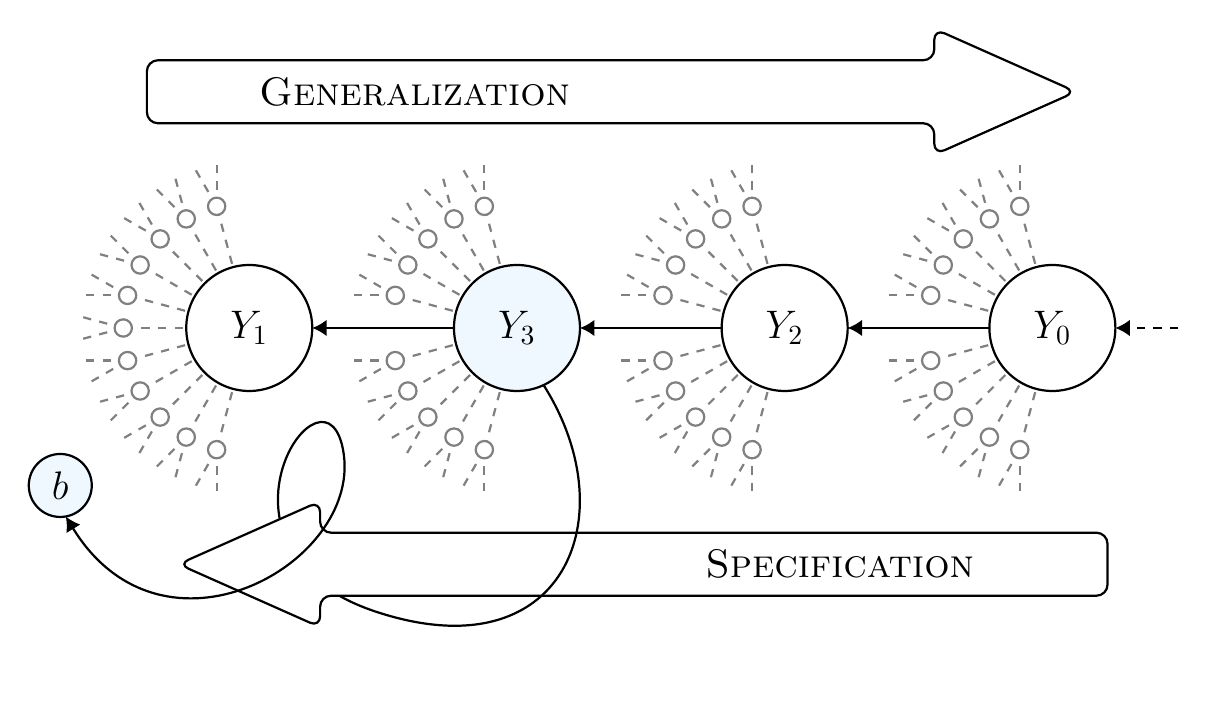
\begin{tikzpicture}[scale=0.2]
		
			%--- GRAY TREES -------------------------
		
		    \foreach \x in {0,...,3}
		        \foreach \y in {1,...,5}{
		            
		            % Big dashed lines
		            \draw [gray,dashed,thick] (\x*17,0) -- ++(90+\y*15:8);
		            \draw [gray,dashed,thick] (\x*17,0) -- ++(180+\y*15:8);
		            
		            % Small dashed lines
		            \draw [gray,dashed,thick] (\x*17,0) ++(90+\y*15:8) -- ++(90+\y*15-15:3);
		            \draw [gray,dashed,thick] (\x*17,0) ++(90+\y*15:8) -- ++(90+\y*15+15:3);
		            \draw [gray,dashed,thick] (\x*17,0) ++(180+\y*15:8) -- ++(180+\y*15-15:3);
		            \draw [gray,dashed,thick] (\x*17,0) ++(180+\y*15:8) -- ++(180+\y*15+15:3);
		            
		            % Small circles
		            \draw [gray,thick,fill=white] (\x*17,0) ++(90+\y*15:8) circle (0.55);
		            \draw [gray,thick,fill=white] (\x*17,0) ++(180+\y*15:8) circle (0.55);
			    }
		    
		    % Extra gray tree for Y_1 at 180 degrees
		    \draw [gray,dashed,thick] (0,0) -- ++(180:8);
		    \draw [gray,dashed,thick] (0,0) ++(180:8) -- ++(180-15:3);
		    \draw [gray,dashed,thick] (0,0) ++(180:8) -- ++(180+15:3);
		    \draw [gray,thick,fill=white] (0,0) ++(180:8) circle (0.55);
		    
		    %--- CURVES AND BIG ARROWS --------------
		    
		    % Curve coordinates
		    
		    % Red
		    \coordinate (R1) at ($(17,0)+(-65:4)$);
		    \coordinate (R2) at (24,-12);
		    \coordinate (R3) at (20,-22);
		    
		    % Blue
		    \coordinate (M1) at (8,-18);
		    \coordinate (M2) at (-4,-14);
		    \coordinate (M3) at (5,-1);
		    
		    % Green
		    \coordinate (L1) at (6,-8);
		    \coordinate (L2) at (7,-15);
		    \coordinate (L3) at (-5.5,-22);
		    \coordinate (END) at ($(-12,-10)+(-80:2)$);
		    
		    
		    % MIDDLE curve
		    \draw [thick] plot [smooth]
		    (M1) .. controls (M2) and (M3) .. (L1);
		    
		    % Big arrows
		    \draw [thick, rounded corners, fill=white] (-6.5,13) -- ++(0,4) -- ++(50,0) -- ++(0,2) -- ++(9,-4) -- ++(-9,-4) -- ++(0,2) -- cycle;
		    \node at (10.5,15) {\Large \textsc{Generalization}};
		    
		    \draw [thick, rounded corners, fill=white] (54.5,-13) -- ++(0,-4) -- ++(-50,0) -- ++(0,-2) -- ++(-9,4) -- ++(9,4) -- ++(0,-2) -- cycle;
		    \node at (37.5,-15) {\Large \textsc{Specification}};
		    
		    % RIGHT curve
		    \draw [thick] plot [smooth]
		    (R1) .. controls (R2) and (R3) .. (M1);
		    
		    % LEFT curve
		    \draw [-{Latex[length=5mm,width=2mm,angle=60:6pt]},thick] plot [smooth]
		    (L1) .. controls (L2) and (L3) .. (END);
		    
		    %--- NODES AND SMALL ARROWS -------------
		    
		    % Arrows
		    \foreach \x in {1,2,3}{
		    	\draw [-{Latex[length=5mm,width=2mm,angle=60:6pt]},thick] (17*\x,0) -- +(-13,0);
		    }
	    	\draw [-{Latex[length=5mm,width=2mm,angle=60:6pt]},thick,dashed] (17*3+8,0) -- +(-4,0);
		    
		    % Y nodes
		    \draw [thick,fill=white] (0,0) circle (4) node {\Large $Y_1$};
		    \draw [thick,fill=textbook-blue] (17,0) circle (4) node {\Large $Y_3$};
		    \draw [thick,fill=white] (2*17,0) circle (4) node {\Large $Y_2$};
		    \draw [thick,fill=white] (3*17,0) circle (4) node {\Large $Y_0$};
		    
		    % b node
		    \draw [thick,fill=textbook-blue] (-12,-10) circle (2);
		    \node at (-12,-10) {\Large $b$};
		    
		    % Bezier curve assistant (used for sculpting curves)
		    % \draw [thick,red] (R1) -- (R2) -- (R3) -- (M1);
		    % \draw [thick,blue] (M1) -- (M2) -- (M3) -- (L1);
		    % \draw [thick,green] (L1) -- (L2) -- (L3) -- (END);
		    
		\end{tikzpicture}
	}
\end{center}

% Diagram -> Generalization/Specification -> Top and Bottom/Type Theory -> Generalization is theory building, specification is theory using -> information is both fundamental and very general -> because it is so general, we need to pull from a lot of fields to properly characterize it.

In the above diagram, we see the $Y$ classes and their relations to each other. The arrows between them are \textit{subsumption} relations. They point from a \textit{parent} class $P$ to a \textit{child} class $C$, and we say that $P$ \textit{subsumes} $C$ (i.e. it encompasses the entirety of $C$). In set theory notation, $P\subset C$. Alternatively, we can reverse the arrows and call them instead \textit{is-a} relations, which point from $C$ to $P$. Every $c\in C$ is a member of the more general class $P$, and thus every $c$ \textbf{is a} $P$ of some \textit{type}. \\

Of course, any given type $T$ can have many \textit{subtypes}, and those subtypes can have their own subtypes. A subtype of $T$ builds on the information that defines $T$, adding new information that further specifies the underlying parent class. And with enough divergent specification, these subtypes may become quite unlike each other at a glance, sharing little else than a distant relation to $T$. This branching nature of subsumption is depicted above in gray. \\

Like branches that furcate from an old oak tree and fork into smaller branches toward the leaves, types spread in a \textit{recursive} manner, each one potentially a parent of arbitrarily many children and an ancestor of arbitrarily long lineages. As a \textit{type system} like this grows deeper and denser, more information is required to represent it. Similarly, any class in the system \textit{gains information} as it is specified and \textit{loses information} as it is generalized. Thus, a class of type $T$ is \textit{also} of any supertype of $T$ because each possible supertype represents a subset of $T$'s information. For example, the class \textit{Car} is of type \textit{Car}, but it is also of the more general types \textit{Vehicle} and \textit{Machine}. \\

Naturally, one wonders about what might happen at the extremes of generalization and specification. Three relevant question-answer pairs are given below: \\

\begin{itemize}
	\item \textit{Is there a type so general that it describes everything?} \\\\	
	Indeed, there is: it is the \textit{top type} $\top$, and it describes a special class known as a \textit{domain of discourse} or \textit{universe}. The names speak for themselves---the supertype of \textit{everything} describes the class of \textit{all things} under discussion, the \textit{universe} of relevant topics, the \textit{domain} of our discourse. $\top$ serves as a useful label in situations when type is unimportant or indeterminate.
	\item \textit{Is there a type so specific that it describes \dots\ nothing?} \\\\
	Yes. It is the \textit{bottom type} $\bot$, and it describes the \textit{empty class}, the class with zero members. It can be considered the type of an \textit{overspecified} class. That is, the class has been defined such that no object in the \textit{domain of discourse} complies. $\bot$ describes things that are \textit{out of scope} or \textit{nonexistent}. Thus, it is often used as the return type of functions that \textit{diverge} (i.e. do not terminate properly) or as the type of \textit{nothing} (e.g. the $5^{th}$ element in a $4$-element list is nothing).
	\item \textit{Are instances just classes that are specified until they have one element?} \\\\
	Technically, no. Specification is a class-to-class process: a class is specified, and a subclass is the result. \textit{Instantiation}, the construction of a concrete \textit{instance} from an abstract description, is instead a class-to-object process. For example, in the above diagram, the class $Y_3$ is \textit{instantiated} in order to produce the object $b$ (or, by reversing the direction of the arrow, we may say that $b$ is an \textbf{instance of} $Y_3$). \\\\
	Because a type describes a class, it is also incorrect to say that $b$ defines its own subtype of \textit{Car}. Rather, $b$ is a \textit{token} of type \textit{Car}, a physical object that \textit{realizes} one of the many possible designs that fall under the class \textit{Car}. However, $Y_3$ could be specified such that $b$ is the sole element of the resultant class ${b}$. A class with one member is called a \textit{singleton class}, and it has a \textit{unit type}, a type with one valid value. The type of ${b}$ would be a subtype of \textit{Car} that describes only $b$, but neither ${b}$ nor its type are the same thing as the \textit{instance} $b$. \\
\end{itemize}

% Generalization is powerful because it allows you to know things about systems you haven't seen before. It gives intuitive understanding.

% We will discuss upper ontologies next. This will inform later discussions on domain ontologies for physics and computer science.

%----------------------------------------

\subsection{Classical Metaphysics}

% Wiki: Natural Philosophy

% What good is (natural) philosophy in an era of such sophisticated science?

% What is... metaphysics (study of structure), epistemology (study of knowledge), logic (study of truth), axiology (ethics and aesthetics, study of value) and phenomenology (study of experience)? Make a fun diagram maybe?
% What is ontology? What is an ontology?
% What do metaphysics and ontology have to do with computers or programming? Or with OOP specifically?

Blah

% The Universe was described imaginatively before it was described abstractly.
% Gods are a good metaphor for natural events. People wanted to describe something that was more powerful than humans and seemingly eternal.
% Polytheistic religions explain the complexity of the world with multiple gods with different personalities and goals. Monotheistic religions lean toward a god that is benevolent (an omniscient, malevolent god is hard to justify, given that we are still alive).
% Religion can serve various purposes: a comfort and a guide in a harsh, confusing world; an explanation of reality and nature; a way to feel one with nature and to find inner peace; a set of rituals that serve to maintain relations between human beings and the tempermental forces of nature; a cultural mythology meant to encourage cooperation between strangers in agrarian civilizations; a promotion of self-discipline and perseverence; an explanation of the vast gap in intelligence between humans and animals; an explanation of subjective experience; an interpretaion of hallucinations induced by schizophrenia or psychedelic drugs; an indulgence in magical thinking and perhaps in the practice of magic; a framework in which one can contemplate personal struggles and express them to a caring parent-figure; a figure to whom one can plead for mercy; a way to process one's own mortality; an assurance that warriors will be rewarded for dying on the battlefield; an interpretation of death such that a future reunion with deceased loved ones is possible; a way to avoid existential crisis and the feeling of meaninglessness; a hope for salvation from this world of suffering; a piece of culture that unites a group of people (and perhaps gives them a sense of superiority); a component of national, cultural, or ethnic identity; an ideological tool used to justify political and social actions; a reason for the congregation of a community; a promotion of nuclear family structure in order to support children; a claim of divine right to rule; a justification for a standard code of ethics; a philosophy that may provide one with a sense of meaning and control.
% Sensus divinitatis, sensus deitatis
% What are the components of a religion? Mythology, ethics, rituals...

% Proto-Indo-European mythology
% Shamanism, totemism, animism, spirit world, animal worship and sacrifice
% From polytheism to henotheism to monotheism (multiple gods means you need more justification). Dyeus. Aten. Really started in Late Antiquity though.
% World egg (Orphic egg), primordial substance, hyle, matter
% Son of God, rulers and kings.
% Axis mundii. It is natural to associate the sky with heaven because it is bright (which humans think is good), endless, beautiful, and mysterious. Thus, a local people will often consider the holiest place of an area to be the highest one (usually a mountain). This is the center of the world, and the connection point between Heaven and Earth.
% Similarly, familiar places that are close to the center are considered better than the dark, foreign lands that are unknown and scary.

% One could argue that philosophy has been done ever since we could think. But philosophy in Ancient Greece was different. Why? Geography. Democracy.
% Yes, other cultures had "philosophies" at this time, but the word in this case is referring to a \textit{worldview}. We are discussing philosophy in the sense of \textit{analysis}.

\subsubsection{\textit{Henosis} and \textit{Arche}}

% Monism and dualism (and other isms) are just simple, broad models or ways of looking at the world

Blah

% Orphism. Dionysus (Zagreus), son of Zeus and Persephone, is dismembered, boiled, and eaten by the Titans (who are "white clay men" covered in gypsum). Athena saves the heart, tells Zeus, and Zeus smites the Titans. The resulting soot is mankind, with both the divine soul of Dionysus and the natural body of the Titans. The heart is then placed within a gypsum statue resembling Dionysus. This religion believed in transmigration of the soul, which Plato later supported.
% In this story, Dionysus may resemble grapes that are ripped from the vine and boiled into wine (divine + vegetation = wine grapes). In Dionysian mystery religion, raving women known as maenads would get drunk on wine and incite themselves into ecstacy (enthusiasm) by shouting and dancing wildly. The dismemberment and devouring of animals (perhaps including humans) was also associated with these cults. Dionysus was depicted by satyrs, who are half man, half beast. These rituals were explorations of the animalistic side of humans. There was much emphasis on becoming one with the god and phenomenal experience.
% Motivation for metaphysics. The One. The Being. The Real. Henosis (the process of unification, unity, or oneness). Henosis is the primordial unification of all things \textit{in perpetuum}, the present and eternal \textit{being} of everything. Henosis is heavily related to the principle of causality. From uncertainty flows the uncaused cause. That is, there is nothing certain at first. Then, something happens, and it causes something else to happen. These events happen relative to each other in space and time.
% The One introduces a fundamental question in Western philosophy: Is there an Absolute? Is reality unified in some way?
% The Romans referred to it as the \textit{universus} (literally, the \textit{turned in one}).
% Arche means origin (first principle, element, the nature). Philosophy was born in asking what the nature of things was.
% Physis (nature, growth) vs. nomos (human convention). The distinction was made maybe because the Greeks had contact with many different cultures interpreting the world in different ways.
% Thales. Explaining things without the supernatural. From many things to one substance (the arche is water). Cultural reasons for choosing water. A distinction between appearance and reality. You can live life according to appearances, but you can also learn for the sake of learning. And it turns out learning can be useful, too (olive story).

% Heraclitus. The arche is fire because it symbolizes change. Flow of time.
% Logos (word, account, principle of order): the great computer program in the sky (or the Word of God, to a Christian).

% Empedocles invents the classical elements.
% Rebooting Hesiod's Theogony. Instead of gods emerging from the Chaos, let's try to categorize everything naturalistically.

\subsubsection{Democritus' Atomism}

Blah

% Time is an instance of the Form of eternity. The Greeks did not think about time like us.
% Atoms come in different shapes that give different properties. The shapes also influence sensory perception (bitter/salty taste comes from sharp atoms).
% Materialism, mechanism, naturalism

\subsubsection{Plato's Theory of Forms}

% Plato hates Democritus. Wants to burn all of his books. Plato's philosophy is an objection to atomism. Believes that there must be something divine about nature due to its beauty.
% Plato is rationalist, Democritus is mechanist and materialist (they agree on epistemology though)
% Plato is a substance dualist. The human soul is an element of the Platonic realm.
% Essence precedes existence. There is inherent meaning in reality.

Plato (c. 428/427 -- c. 348/347 BCE) was the first to expound a metaphysics of objects with his \textit{theory of Forms}, which proposed a solution to the \textit{problem of universals}. This problem is subtle, but important: how can one general property appear in many individual objects? For example, when we say that a floor and a bowl are \textit{smooth}, are we referring to some singular paradigm of \textit{smoothness} that is independent of each? For Plato, \textit{universals} or \textit{Forms}, such as smoothness, are indeed distinct from the \textit{particulars} that \textit{partake} of them, such as floors and bowls and other smooth objects. He posits that the \textit{essence} of an object, its \textit{sine qua non}, is the result of its partaking of these Forms. \\

\textit{Forms}, as conceptualized by Plato, are ideal, abstract entities that exist in the \textit{hyperouranos}, the realm beyond the \textit{heavens}. In the times of Homer and Hesiod, the Ancient Greeks understood a cosmology that closely mirrored that of the Hebrew Bible. They envisioned the Earth as a flat disc surrounded by endless ocean and the sky as a solid dome with gem-like stars embedded in it, much as it all appears from a naive perspective on the ground. Under the Earth was the \textit{underworld}, where the dead live, and beyond the dome were the \textit{heavens}, where the divine live. \\

% Elaborate on why spheres were chosen. The Universe was also a sphere.

Plato, however, was influenced by the philosophy of Pythagoras (c. 570 -- c. 495 BCE), who championed a spherical Earth for aesthetic reasons. Thus, he instead modeled the Earth as a "round body in the center of the heavens," and he imagined the Forms as part of a different, eternal world that transcends physical space and time. Whereas physical reality is the domain of perception and opinion, the realm of the Forms is, as he paints it in \textit{Phaedrus}, the domain of \textit{reason}: \\

\begin{displayquote}
	Of that place beyond the heavens none of our earthly poets has yet sung, and none shall sing worthily. But this is the manner of it, for assuredly we must be bold to speak what is true, above all when our discourse is upon truth. It is there that true Being dwells, without colour or shape, that cannot be touched; reason alone, the soul's pilot, can behold it, and all true knowledge is knowledge thereof. Now even as the mind of a god is nourished by reason and knowledge, so also is it with every soul that has a care to receive her proper food; wherefore when at last she has beheld Being she is well content, and contemplating truth she is nourished and prospers, until the heaven's revolution brings her back full circle. And while she is borne round she discerns justice, its very self, and likewise temperance, and knowledge, not the knowledge that is neighbor to Becoming and varies with the various objects to which we commonly ascribe being, but the veritable knowledge of Being that veritably is. And when she has contemplated likewise and feasted upon all else that has true being, she descends again within the heavens and comes back home. And having so come, her charioteer sets his steeds at their manger, and puts ambrosia before them and draught of nectar to drink withal. \\
\end{displayquote}

Plato makes a revolutionary statement here about the nature of scientific knowledge. He declares that one cannot know the physical world directly because it is, in fact, \textit{less real} than the \textit{hyperouranos}. As he puts it in \textit{Timaeus}, a Form is "what always is and never becomes," and a particular is "what becomes and never is." Further, physical reality is merely the "receptacle of all Becoming," a three-dimensional \textit{space} that affords spatial \textit{extension} and \textit{location} to all particulars. Unlike Forms, particulars are subject to \textit{change}, and thus cannot be sources of absolute knowledge. They are slippery, metaphysically undefinable, and explainable only in terms of the unchanging Forms of which they partake. \\

% Plato's criticism of Heraclitus' conception of time (wiki Heraclitus)

The above passage can be interpreted as an early argument for basing human knowledge in abstract mathematics rather than in subjective evaluations of concrete observations. For example, to \textit{know} what a triangle is, one cannot simply point to a triangular rock or even to a very carefully drawn diagram of a triangle. One must instead use \textit{abstract reasoning} to express the Form of a triangle by means of a \textit{formal definition}: a three-sided shape in a two-dimensional plane. This is the \textit{essence} of a triangle. In contrast, the triangular rock and diagram each partake of multiple Forms, and neither are perfectly triangular. We may still \textit{call} them triangles, but only those who know the Form of a triangle will understand what we mean when we do so. Therefore, it is knowledge of the unambiguous Form that gives insight into the complex and ever-changing particular, not the other way around. \\

Here, our object-property distinction blurs. Because while Forms may define universal properties, are they not also objects in an abstract sense? And while concrete particulars may be objects, are they not also fully characterized by a set of properties? In Plato's metaphysics, the categories of interest are really the \textit{concrete} and the \textit{abstract}, that which we \textit{perceive} and that which we \textit{conceive}. Plato further claims that humans come from the abstract realm, where they familiarize themselves with the Forms, and they are born into the concrete realm, where particulars are abundant and Forms are only latent memories. It is through philosophy then, the exploration of the rational mind, that we unearth our innate understanding. \\

To explain the link between the realms, Plato also postulates a \textit{demiurge}, a transcendent artisan who shapes an initially chaotic space into an ordered, material reality, using the Forms as models. This entity is benevolent and wishes to craft a world like the ideal one he sees, but the objects that he \textit{instantiates} are always imperfect copies. Like that of a master portraitist, his work is beautiful, but it is, in the end, a mere \textit{image} of his subject. \\

So it is for programmers. Before us lies the space of computer memory, uniform and featureless, a receptacle of Becoming. Our Forms are \textit{types}, our particulars are \textit{values}, and the behavior in the space is dictated by the \textit{code} that we execute. In \textit{object-oriented programming} (OOP), values can be of an \textit{object type} that is formally defined by a \textit{class}. \\

For example, my cat Mystic belongs to the class of entities known as Cat, the set of all possible cats. She is an \textit{object} known as a cat, and her catness is defined by the class Cat. In Plato's terms, she is a \textit{particular}, partaking of the Form \textit{Cat}. Just as the demiurge instantiates particulars from Forms, so the programmer instantiates objects from classes. Both bridge the gap between what is possible and what is. \\

That said, while Plato's metaphysics gives good insight into OOP and other abstract (or \textit{high-level}) programming concepts, it cannot explain concrete (or \textit{low-level}) ideas like \textit{data} that is represented with \textit{bits}. This is because Plato was not overly concerned with the \textit{substance} of objects, the stuff that makes them \textit{physical}. Thus, in our pursuit of a holistic understanding of \textit{information}, we must also consider \textit{substance theories}, philosophies that give metaphysical weight to \textit{matter}. \\

% Plato associates the classical elements with the Platonic solids. He argues that they are not atoms but corpuscles (sort of). Also, the elements are not the arche because they are material.
% Plato not very interested in matter. His arche is immaterial (triangles), not material (atoms).
% Plato indentified The One with \textit{The Good}. Through philosophy, one uses the Nous to find the truth of the Good. The Good is the Form of Forms. It is the ultimate object of knowledge that allows one to realize all other Forms. It allows us to comprehend justice. The Good is why there is "divine order" to reality. It is the reason why things are intelligible and are not just chaos. The Good is also the reason philosophy and science are possible.

% The Good is the Form of goodness. A thing's goodness is its purpose (or telos). Teleology.
% The Good is the point of philosophy. There is reason to believe that there is way to exist and think that is good. We can find it with philosophy.
% Aristotle's eudaimonia ("good spirit," human flourishing or prosperity).
% Pirsig's Metaphysics of Quality
% Stoicism

% Neoplatonism
% The Monad (The One, The Good) is the possibility of existence (dunamis).
% The Nous (The Intellect, Mind, Reason) is God or the Demiurge (thinker and composed of thought, divine order, structure instead of chaos). It is an energeia (a thing at work) that actualizes these thoughts as the Forms.
% The Soul (Psyche, Pneuma, Breath, Fire, World Soul) is an energeia that actualizes thoughts into existence: it creates a material, living cosmos in the image of the mental Cosmos that is a unified thought within the Intellect (a system of Forms).
% Logos is the principle of meditation, which relates the One, the Intellect, and the Soul (the hypostases) to each other.
% Eros is ideal love, a love for inner beauty. It is the path to divinity, a desire to possess the Good forever, a desire for immortality.

% The Christian Trinity is similar:
% The Godhead is the Good (the divine substance).
% The Father is the Nous, the Son is the Logos (Word), the Holy Spirit is the Pneuma (Breath).
% The metaphor is: there is a Divine Creator (or Mind), and he created everything with the Word (a speech composed by a rational mind) which he executes by means of Breath or Soul (the hot air of life). Just like a Programmer creates a Program that he executes by means of Computation.
% Speech scroll

\subsubsection{Aristotle's Hylomorphism}

Blah \\

% Aristotle is sort of a mixture of Democritus and Plato. Not entirely materialist, but not fully abstract. It's scientific, but also teleological. Democritus embraces physis, Plato rejects it, and Aristotle redefines it. Physis is defined by the four causes. Nature and art are both part of physis, but the latter requires an external force/motion. Thus, the natural world has a "soul."
% Aristotle did not have a singular arche. But he wrote about minima naturalia, the most fundamental of which were the matter + form combos of the classical elements. He did not believe in a void, reality was continuous (big effect on physics and mathematics).

% Substance != matter for Aristotle.
% Rejects atomism, says reality is continuous (corpuscles)
% Rejects an immaterial fundamental unit, believes substance is real
% Four formal causes
% Potentiality and actuality (properties of the formal realm and the physical realm, respectively).
% Objects are characterized spatially, events temporally.
% Mathematical objects and operators
% Plato is rationalist, Aristotle is empiricist

% "We (collectively, as humans) bestow globality on first principles inductively, promoting the said principles to the status of universal, often missing meaningful alternatives in the process." -- Alon Amit
% Put this after Euclid's section?

%----------------------------------------

\subsection{Theories and Models}

% Instrumentalism

% Patterns

% "Models of computation" (coming up in section 3)

% Can we say anything objectively about the structure of the Universe? For example, can we say for certain that the Universe is continuous or discrete? Probably not. But we can build some very sophisticated theories and models that describe the Universe very well.

% Wiki: analogical models
% Medium - mechanical, electrical
% Cardinality - N_0 is digital, N_1 is analog
% Scope - specific-purpose vs. general-purpose

% Axiomatic system -> theory -> model -> simulation

% System - a bunch of interrelated parts
% Theory - a way of looking at a system (syntactic, system-independent, but perhaps designed with the system in mind)
% Model - a way to represent a system (or the application of a theory to a system)

% Theoria vs. praxis (considering things outside of our control vs. considering things we can change)
% Pythagoras considered theories a way of contemplating math

% Scientific disciplines use math to describe parts of reality "in certain terms." Two scientific disciplines might describe the same thing from different vantage points. Theories as models. Scientific laws are not axioms. Models represent reality in some, but not all, ways. If they represented everything, they wouldn't be models. They would be the thing itself. In mathematical models of physics, statements represent physical phenomena.
% Theories that describe the same phenomena may differ based on what their basic abstract objects are (particles, waves, bits). These objects are reference points, helpful abstractions inspired by previous observation.
% Logic/math theories have axioms/postulates and theorems about formal phenomena and are interpretation-independent. Logic/math models are particular algebraic structures, abstract objects that satisfy a theory (e.g. a set S is a model of set theory, a group G is a model of group theory)
% Scientific theories have postulates and laws/principles about natural phenomena. Laws are classical and are expressed with formulas. They are not certain, but are rather extremely probable and backed by mountains of evidence. Principles are modern and are expressed in words. They are "guiding ideas" and do not require proof. Principles can be violated, but you better have good reason to suspect that's the case.
% Axioms vs postulates. Essentially synonymous, but the former is more common in math and the latter is more common in science. Mathematicians do not consider axioms verifiable. In science, postulates are about the physical world, and physics is verifiable, so postulates are verifiable. Postulates can be broken if contrary evidence is found.
% Models do not *exist*. They are mathematical abstractions that describe reality. Some phenomenon might be "well-described" by a theoretical model, but that does not make it a signal, field, etc.
% Table for model classifications: linear/non, static/dynamic, explicit/implicit, discrete/continuous, deterministic/probabilistic, deductive/inductive/floating
% Models may die out if they have major flaws. However, crude models are still sometimes useful due to their simplicity (classical mechanics).
% Theories are abstract models, models whose components are symbolic.

% A model represents a system, a simulation represents its operation over time.
% A computer program can be interpreted as a simulation of some aspect of the Universe and, at the time, as a little Universe in and of itself. The difference between this universe and \textit{the} Universe is that we theoretically have access to all of the information in the former. Whereas we are babies stumbling around in the dark of physical reality, we are gods of the universes we architect in digital memory.
% Mindset (blue box?). You can think of programming as just sitting at a desk and typing a bunch of obscure mumbo jumbo. Or you can think of it as the means to simulate anything that you want.

% Systems (language systems, logical/formal systems, algebraic systems, automatic systems, hardware systems, software systems, operating systems). All of these can be modeled in terms of information.

Blah

\subsubsection{Euclid's \textit{Elements}}

Although arithmetic has been practiced since prehistory, theoretical mathematics was founded by the Ancient Greeks. The Greeks, in contrast to earlier peoples, applied \textit{deductive reasoning} to the study of mathematics. While sophisticated arithmetic, geometry, and algebra was done before this period by the Babylonians and the Egyptians, this work was all based on \textit{evidence} collected from the physical world. The Greeks were the first to recognize the need for \textit{proof} of mathematical statements using \textit{logic}. \\

% Euclid used axiomatic and constructive methods
% Axioms come from Aristotle, formal definitions come from Plato

While various proofs were written by Greeks in the centuries before his birth, Euclid of Alexandria is nonetheless credited with formalizing the concept of proof due to his use of the \textit{axiomatic method} in his groundbreaking treatise, \textit{Elements}. This work was the first of its kind, serving as both a comprehensive compilation of Greek mathematical knowledge and as an introductory text suitable for students. Additionally, it was a product of a synthesis of Greek thought, founded on the epistemology and metaphysics of Plato and Aristotle. \\

\textit{Elements} is divided into thirteen books. Books I--IV and VI cover \textit{plane geometry}, the study of shape, size, and position in two-dimensional space. Books V and VII--X cover elementary \textit{number theory} (classically known as \textit{arithmetic}) in a geometric way, expressing numbers as lengths of line segments. Finally, Books XI--XIII cover \textit{solid geometry} by applying principles of plane geometry to three-dimensional space. Each book begins with a list of \textit{definitions} (if necessary) that assign names to abstract mathematical ideas that are expressed in unambiguous terms. These ideas are then used to prove \textit{propositions}, mathematical statements that warrant proof. \\

Euclid's proofs in \textit{Elements} can be described as \textit{axiomatic}. That is, they start from \textit{axioms}, statements that are taken as true without proof. Axioms solve a problem in logical argumentation known as \textit{infinite regress}, which often occurs, for example, when children ask questions. A curious child, seeking knowledge, might ask his parent why something is the way it is. That is, he requests a proof of some proposition $P_0$. The parent would respond with some proposition $P_1$ that supports the truth of $P_0$. The child, unsatisfied, would subsequently ask why $P_1$ is true. The parent would respond with the assertion that $P_2$ is true and implies $P_1$, and the child would similarly question whence $P_2$ arises. This dialogue could continue in this manner forever with the child endlessly searching for an anchor with which he can ground his understanding. However, patience waning, the parent must end this line of questioning by giving an unquestionable answer. Common examples include "Because that's just the way it is" or "Because I said so." \\

Some Greek philosophers considered infinite regress to be a serious epistemological issue. If we assume that all knowledge must be demonstrable by a proof or logical argument, we cannot know anything because our axioms cannot be satisfactorily proven. And yet, there are things that we claim to know. In his \textit{Posterior Analytics}, Aristotle challenges this notion that all knowledge must be provable, averring that \\

\begin{displayquote}
	All instruction given or received by way of argument proceeds from pre-existent knowledge. \\
\end{displayquote} 

Aristotle continues his text in support of this statement. He discusses the nature of \textit{premises} in his \textit{syllogistic logic} and how they differ from the \textit{conclusions} that they derive. Namely, he states that the premises of a knowledge-producing deductive argument or \textit{syllogism} must be \textit{true}, to ensure the truth of their conclusion, \textit{indemonstrable}, to ensure that they are independent of proof, and \textit{causal}, to ensure that their conclusion logically follows: \\

\begin{displayquote}
	Assuming then that my thesis as to the nature of scientific knowledge is correct, the premises of demonstrated knowledge must be true, primary, immediate, better known than and prior to the conclusion, which is further related to them as effect to cause. Unless these conditions are satisfied, the basic truths will not be 'appropriate' to the conclusion. Syllogism there may indeed be without these conditions, but such syllogism, not being productive of scientific knowledge, will not be demonstration. The premises must be true: for that which is non-existent cannot be known---we cannot know, e.g. that the diagonal of a square is commensurate with its side. The premises must be primary and indemonstrable; otherwise they will require demonstration in order to be known, since to have knowledge, if it be not accidental knowledge, of things which are demonstrable, means precisely to have a demonstration of them. The premises must be causes, since we posess scientific knowledge of a thing only when we know its cause; prior, in order to be causes; antecedently known, this antecedent knowledge being not our mere understanding of the meaning, but knowledge of the fact as well. \\
\end{displayquote}

Thus, Aristotle differentiates \textit{pre-existent knowledge} from \textit{scientific knowledge}. Whereas the latter is produced by means of a logical proof, the former is produced by one's \textit{intuition}. He goes on to argue that what we intuitively understand is indeed knowledge, in the same way that what we prove is knowledge. The difference, he argues, is that axioms are \textit{self-evident}. For example, the reflexive property of the natural numbers (i.e. for every natural $x$, $x=x$) is typically considered so obvious that proof is unnecessary. At the same time, the statement is so fundamental that it cannot really be proven. Despite their unprovability, Aristotle argues that axioms such as these constitute knowledge that is simply, unquestionably \textit{known}: \\

\begin{displayquote}
	Our own doctrine is that not all knowledge is demonstrative: on the contrary, knowledge of the immediate premises is independent of demonstration. (The necessity of this is obvious; for since we must know the prior premises from which the demonstration is drawn, and since the regress must end in immediate truths, those truths must be indemonstrable.) Such, then, is our doctrine, and in addition we maintain that besides scientific knowledge there is its originative source which enables us to recognize the definitions. \\
\end{displayquote}

Euclid apparently agreed with this epistemology because Book I of \textit{Elements}, in addition to its definitions and propositions, contains a number of axioms, which are labeled either as \textit{postulates} or \textit{common notions}. In antiquity, a postulate denoted an axiom of a particular science, whereas a common notion denoted an axiom common to all sciences. Today, we do not think of axioms in this way. Rather, we simply consider them starting points for proofs. Euclid's axioms are given below: \\

\begin{center}
	\textbf{Postulates}
	\begin{enumerate}
		\item Hi
	\end{enumerate}
	\textbf{Common Notions}
	\begin{enumerate}
		\item Hi
	\end{enumerate}
	
\end{center}

Euclid's proofs can also be described as \textit{constructive}. \\

% Aristotle's logic was two-valued. However, he did not fully accept the law of excluded middle.

% The Greeks used geometry to get around the precision errors of irrational numbers. That's why they used line segments to teach arithmetic.

% Elements is great and super important, but in some ways it held mathematics back. It was taught for over 2000 years, and many people assumed it could not be wrong. In fact, it is not considered formal by modern standards, and it is not a general theory of geometry. Critique of the 5th postulate. Non-Euclidean geometry, postulates of special relativity, Galois theory, modern mathematics does not treat axioms as "self-evident" but rather as starting points. Elements assumed many things to be generally true, which are not: numbers are one-dimensional, mathematical objects must be constructed, mathematics must describe the world as we observe it (2d/3d space, concrete objects), mathematics requires straightedge and compass construction, there is only one way to describe geometry. None of these are true, and modern mathematics began when people started questioning Elements.

% Aristotle's metaphysics influences science for 2000 years.

% Aristotle's ten categories
% Moving away from Aristotelian realism, Kant supposes that categories say something about how we conceptualize reality, not about reality itself.

%----------------------------------------

\subsection{Modeling Physical Reality}

% Religion, mythology, cosmogomy
% We're not going to deeply discuss religion or any theory that says more about the supernatural than the natural. However, we will briefly touch on some ancient models of physical reality that are intertwined with spirituality.
% Touch on religion up front, so we don't have to talk about it after this.
% Models are constructed within the "religion" of a society. This is not religion in the customary sense, but a spiritual, cultural bias, a set of guiding ideals. Heisenburg calls it the "spiritual pattern of a community." Religion in this sense does not have to be theistic.
% "Two kinds of truth"
% Religion helps us make sense of the chaos. A common theme is a belief in The One, an interconnection of seemingly disparate things.
% The progress of science was held back by war, disease, and also religion. But religion is not inherently destructive. Science and religion discuss two entirely separate things. The mistake was in trying to fit science into a religious model. Too many scientists spent time looking for rigid patterns in the Universe that meshed with their religion, and they just were not there. The Universe is not a divine puzzle that holds the meaning of the divine.
% In the same way that there are scientific things that religion has no bearing on, there are religious things that science has no bearing on (ethics). Science will not make religion obsolete. Humans need meaning, community, fulfillment, guidance, etc. Technology does not solve these things. Religion does (however, again, it doesn't require God).
% We see a trend from anthrocentric to not. We are biased toward our species, our intelligence, our planet, our culture, our language.
% The cardinal sin of religion was making something personal into something societal.

\subsubsection{Pre-scientific Thought}

% One paragraph MAX for each idea.

% Atomic theory of Hindu philosophy
% Tao, Yin and Yang
% Indra's net
% Monad, Pythagoreanism
% Classical elements, aether
% Pre-Socratic atomist philosophy
% And then came Socrates, Plato, and Aristotle
% Kosmos and Nous, Plotinus

% And then came post-Antiquity...
% Why is it important to talk about this period that is often termed the "Dark Ages"? Well, one reason is that all of the glorious classical knowledge was "lost" for a while outside of Constantinople. Western Europeans had to \textit{discover} the lost knowledge of their ancestors, and they thought very highly of these texts. As we nowadays might opine in favor of "the glory that was Greece, the grandeur that was Rome" (Poe's words, not mine), these peoples revered this knowledge. The trope is common in science-fiction---a lost, ancient civilization, beautiful culture and technology in ruins, far more advanced than what is presently known---but it does appear in history as well, given the right context. Other civilizations (namely the Islamic ones) discovered the knowledge through trade and also valued it, and they built on it in incredibly innovative ways (algebra, combinatorics).
% Rome comes and goes, classical knowledge is lost to the West for hundreds of years, but is preserved in Byzantium/Constantinople (Nova Roma)
% Christianity dominates the Western world and academic work is done primarily in order to support Christian theology. Naturalism dies out.
% Constantine I - lots of Christian theological stuff happens in Constantinople.
% Some scientific work is done in the West during the Middle Ages, but it is isolated and there is little progress. Less than 1% of the world is literate.
% Justinian I and the Plague of Justinian
% Charlemagne the Great - the revival of learning
% Islamic Arabs seek out and acquire the knowledge of other civilizations, Classical Greek knowledge is acquired from Constantinople, Translation Movement, the Islamic Golden Age occurs, ends due to the destruction of Baghdad by Mongols
% Europe slowly recovers Ancient Greek knowledge, and academic work is done to harmonize Aristotelian thought with Christianity
% The Black Death happens and wipes out half of Europe, scientific work halts
% Constantinople falls to the Ottomans in 1453, Byzantine scholars flee to Europe, bringing their knowledge of algebra
% The invention of the printing press allows for the wide distribution of information
% A major religious schism occurs in Western Christianity (Protestant Reformation), prompting rebellion in science as well
% Copernicus publishes De Revolutionibus in 1543 on his deathbed
% Galileo champions heliocentric theory and is persecuted by the Church for it. "And yet it moves." Galileo's ship.
% The Scientific Method (Bacon, Descartes, Galileo, Newton) (wiki history of sm)

\subsubsection{Point Particles and Forces}

% Wiki - Meditations on First Philosophy (Descartes discards all he knows and develops a new metaphysical theory from first principles). Powerful statement on the importance of doubt.
% Descartes publishes the idea of a "frame of reference" in 1637 (Fermat also discovers it).
% Descartes founds the rationalist, mechanistic philosophy that early models adhere to (1644). Newton publishes the Principia in 1687.
% Descartes develops the idea of a system.
% Basic assumptions based on observation: continuity, determinism, casuality, forces result from collision, absolute space and time
% Mechanics - study of the behavior of point/body/bodies subjected to forces
	% Statics - the net force is 0, the net work is 0, the body does not accelerate (at rest or constant velocity)
	% Dynamics - nonzero net force, nonzero work, the body accelerates
		% Kinematics - study of motion of a body without considering cause of motion (no masses, no forces, just motion)
		% Kinetics - take cause into account
% In Newton's era, physics was described in terms of bodies, things with mass (atoms, particles, objects). Scientists followed a mechanistic philosophy (physical reality is simply the motion and collision of matter, the universe is deterministic). Newton was a mechanist as well, but made an exception for gravity, which exhibited "action at a distance." He did not attempt to explain gravity, but simply argued that it matched the data.
% Newton discovered that objects would continue their motion if absent of friction, which is a pretty unintuitive idea, considering that there is always friction on Earth.
% Optics - Descartes says light is emitted by sources, Huygens develops a longitudinal wave theory of light transmitted though aether, but people don't believe it because it did not explain birefringence, Newton develops corpuscular theory of light and people accept that.

% Lagrangian Mechanics
% Hamiltonian Mechanics

% Blue box for Hume's Problem of Induction and Kant's Trancendental Aesthetics.
% Hume states that induction is not infallable and thus is unjustified. Kant argues that while it is not infallable, it is still necessary and rational. Kant backs up the scientific method but argues that it does not constitute an objective truth. Science is not certain, but that's okay.
% Critique of Pure Reason - there are other ways of being rational besides deduction
% We can only have knowledge of what appears to us, not of things in themselves.
% Synthetic a priori knowledge (the knowledge of metaphysics) is what allows us to compute mathematics in our heads. Math is necessary and universal, and math can connect a concept to a new concept other than itself (ampliative).
% Religious implications of transcendental idealism
% Kant thinks S+T are just human projections. Synthetic a priori. They require no observation and are projected onto surroundings.
% Kant: nothing about the object's location describes the object itself.
% Walking in a thick grove of trees and finding an overlook into the mountains. Your sense of spatial scope changes. Your mind readjusts.
% Define phenomena, noumena, thing-in-itself

\subsubsection{Waves and Fields}

% In early 1800s, people realize Newton's theory does not explain diffraction, interference, and polarization (physical optics). Young and Fresnel develop a transverse wave theory of light. This is still a mechanistic theory, and, thus, it required an aether (as discussed by Aristotle). People tried to understand how an aether could exist if the Earth moves freely through it. Aether drag and wind theories emerge.
% Similar theories involving mysterious substances ("imponderable fluids") were formed to explain heat and electricity. Faraday proposes that reality is made up of "lines of force." Maxwell agrees and develops an electromagnetic field theory, but he assumes an aether is required.
% Michelson-Morley experiment discredits the aether. Lorentz and Poincare forms a theory with a motionless aether that does not interact with matter. In this case, the aether was more of a reference frame. Length contraction and "local time."

% "Old quantum theory"
% Einstein introduces special relativity, which does not require the concept of aether. Time dilation instead of local time. This theory could be explained in terms of an aether though. The vaccuum of space is more like an aether than a true vaccuum.

% Poincare LET quotes

% Macroscopic physics is now modeled with relativistic mechanics. It is usually described with Lagrangian/Hamiltonian mechanics/field theories.

\subsubsection{Quantum States and Operators}

% Wiki: Mathematical Formulation of the Standard Model

% There was and is a common ethos among professors of quantum mechanics that you should not try to interpret QM as you are learning. The relevent quote comes from David Mermin: "Shut up and calculate!" Many modern physicists disagree. We will approach it in the same way that we approach everything else in this text.

% Modern physics (macro and micro) is described with the Standard Model (quantum mechanics + QFT). This model is imperfect.
% Relativistic, quantum, and quantum field models are applied in different situations depending on the scale of space and time involved. Relativistic mechanics encompasses classical mechanics. It's just more complicated, so classical is still used by humans in situations where relativistic effects are negligible. Scientific computing has no reason to use classical though.
% Energy is transfered due to colliding particles or radiation. The former is modeled by particle theories, the latter by field theories.
% Mass-energy equivalence. Stationary objects have energy because mass is a manifestation of energy. Particles are not necessarily pieces of mass. They are more generally pieces of energy (quanta).

% "The principle of the conservation of mass [...] proved inadequate in the face of the special theory of relativity. It was therefore merged with the energy conservation principle—just as, about 60 years before, the principle of the conservation of mechanical energy had been combined with the principle of the conservation of heat [thermal energy]. We might say that the principle of the conservation of energy, having previously swallowed up that of the conservation of heat, now proceeded to swallow that of the conservation of mass—and holds the field alone. - Einstein
% Time dilation, causality
% The principle of complementarity. Mass and energy (momentum) describe the same thing in different ways. Physics was originally skewed toward the mass view because it is more intuitive and concrete for humans.
% In general, outdated models tend to be anthropocentric in scale for space, time, and semantic meaning (theology). However, less general theories are not "broken." They are still useful in certain scenarios (domains of applicability).
% At small scales, things are unpredictable. They don't really follow laws. Things happen with certain probability. Classical laws are just averages of tons these probabilities from the same distribution, and thus, at human scale, objects behave basically the same way every time. The probability average is extremely close for each test.
% "You can't step into the same river twice." Likewise, classical physics does not behave in exactly the same way twice. We do our best to show general trends, but the Universe is not certain.

% In some sense, quantum mechanics supports object/event metaphysics. Fermions and bosons. Quantum fields of mass and force. Spacetime. Mass-energy. Identical particles.
% QM introduces a conflict over scientific realism. Should scientific theories strive to literally describe reality?
% Bose and Fermi statistics harkens back to Descartes mind-body duality.

% Because QM is probabilistic, this implies that physics is nondeterministic. According to QM, we will never know the true nature of reality with certainty. We cannot know everything about every elementary particle.

% Problems with quantum entanglement. With the Copenhagen interpretation, we maintain that models are NOT reality. Just because the math asserts that some real physical quantity has some value, this is not certain without actually performing a measurement. Theories cannot predict values with absolute certainty.
% EPR paradox. Bell's theorem. QM seems to say things that are impossible. Throwback to Galileo: "And yet it works."
% BIG POINT: It is no longer possible to adhere to both the principle of locality (that distant objects cannot affect local objects), and counterfactual definiteness, a form of ontological realism implicit in classical mechanics. You can only choose one of three: locality, CFD, and conspiracy (that nature only allows researcheer to discover what it wants us to discover). Most people choose locality (because non-locality is contrary to the principle of relativity) and accept that things only exist definitely when they are measured/observed. This is not exactly the same as saying that things are not real, just that we cannot assume that things exist when we are not observing them (e.g. there is no basis in me assuming that Paris exists right now because I am not currently observing it).
% Virtuality is perhaps a more accurate word than reality. That is, we can say that the things that we observe have certain virtues, but we can't assume anything more. The phenomenology of synthetic experience is consistent with that of ordinary experience. Virtual reality is "real" in the same way that the world is "real."
% "'[W]e have to give up the idea of realism to a far greater extent than most physicists believe today.' (Anton Zeilinger) .... By realism, he means the idea that objects have specific features and properties — that a ball is red, that a book contains the works of Shakespeare, or that an electron has a particular spin ... for objects governed by the laws of quantum mechanics, like photons and electrons, it may make no sense to think of them as having well-defined characteristics. Instead, what we see may depend on how we look."

% Copenhagen interpretation claims that QM is a way of acquiring knowledge, but it does not attempt to describe objects in the way that classical mechanics does. It asserts that founding a model on entities or distinctions (such as particles, waves, and bodies) that are intuitive but ultimately unknowable, leads to incorrect predictions somewhere. Instead, it tries to make claims only about things that can be empirically observed.
% Conjugate variables (mass and momentum, uncertainty principle). Derivatives of action. Fundamental interactions. 
% Beyond the standard model: supersymmetry, integrating gravity: string theory, gravitons

% But there is an alternative way of looking at physics that is quite different from the models presented so far...

%----------------------------------------

\subsection{Information Theory}

% A pattern as defined in terms of information (Alon Amit). We study patterns in math and use them to model what we observe in physics. All patterns in the physical world can be described by information.

% How would you describe a beautiful gown with information?

% Bits and bytes and other units of information.
% The base-2 metric system (kibi,mibi,gibi,...)
% The scale of objects - an essay, a book, an encyclopedia, a 1080p photo, a 4K photo, a 1 minute 1080p video, a 1 minute 4K video, a 1080p movie, a 4K movie, an operating system (Linux vs Windows size), programs (little clients to massive environments like modeling softwares), etc.

% If physical phenomena are interpreted as information, this gives formal meaning to the philosophical idea that "we know very little." Much more physical information goes unnoticed than noticed.

% Information is similar to energy transfer. It was compared to theories of heat transfer done during the industrial revolution. When you do work, you give some of your energy to something else. The energy may also be interpreted as changing type (kinetic, chemical, etc.). However, this is also just an abstraction. Energy is energy. There are no types really.
% For example, when you throw a baseball, you transfer chemical energy in your body to kinetic energy in your arm and then you transfer that kinectic energy to the ball. During energy transfer, some of the energy becomes heat. But really, it's all the same energy. You transfer energy to the ball, and most of the energy manifests in motion, but some of it manifests in heat. Efficiency, then, is the ratio of how much of the energy involved is doing what you want it to.

% Entropy - transformational content of energy
% Boltzmann entropy, thermodynamic entropy, von Neumann entropy

% Mathematical theory of communication, Shannon-Weaver model
% What does it mean to be a good communicator?

% Blue box on what it means to have an information-theoretic view of the world. Give multiple examples that do not involve anything digital.
% If you are in possession of information that incriminates you, you want to prevent its communication. You can do this by destroying it (rendering it unintelligible to anyone), encoding it (rendering it unintelligible to people without the decoding algorithm (or code breakers)), encrypting it (putting it in a safe or hiding it), etc.
% If you have space or time constraints, you want to use language that is dense with meaning. You can do this with compression in space (removing all of the vowels, using acronyms and Emojis, using shorthand) or compression in time (writing in cursive, no decorations, ). Often, compression techniques naturally save both time and space (not only do smaller files take up less space, they also download and upload faster).

%--------------------------------------------------------------------------------
%    SECTION: INFORMATION AND COMMUNICATION
%--------------------------------------------------------------------------------

\toclineskip
\section{Information and Communication}

\vspace{4mm}
\begin{displayquote}
	\textit{For Wiener, entropy was a measure of disorder; for Shannon, of uncertainty. Fundamentally, as they were realizing, these were the same.}
	\vspace{2mm}
	\begin{flushright}
		---James Gleick
	\end{flushright}
\end{displayquote}
\vspace{4mm}

% Semiotics
% Signal processing (analog and digital)
% Language
% Coding theory

Blah

%----------------------------------------

\subsection{Signals and Systems}
% Signals are messages composed of time-amplitude data

Data are the building blocks of \textit{signals}, which are mathematical models of quantities that change over time. Signals are carriers of \textit{information} about these quantities. A piece of information, known as a \textit{message}, is encoded as data of a certain \textit{medium}, either physical or numerical. In this sense, one can consider information a meaningful pattern that is embedded in a phenomenon. Philosophically, information is the \textit{essence} of a \textit{substance}, a set of properties that defines what a thing is. Mathematically, signals are functions $f$ that map a set of times $t$ to a set of amplitudes $A$, and they are classified according to the properties of these sets. \\

Sample rate is a property that is related to time. \textit{Continuous} signals are functions of continuous time. That is, $t$ is either the real number line $\mathbb{R}$ or an interval of it. In this case, $t$ is also called a \textit{linear continuum}. This definition of continuity is different from those given in real analysis, which describe functions for which sufficiently small changes in input result in arbitrarily small changes in output. For this reason, these signals are also called \textit{continuous-time} in order to avoid any confusion with the continuous functions that are described in mathematics. If a signal is not continuous, it is \textit{discrete} or discrete-time. \\

Continuous signals that have an infinite number of possible amplitude values (i.e. those that are modeled by $\mathbb{R}$ or $\mathbb{C}$) are called \textit{analog} signals because an infinite-valued output can be viewed as \textit{analogous} to the seemingly infinite complexity of real-world phenomena. At any instant in its time domain, an analog signal can \textit{exactly} model a time-varying, real-world quantity, such as voltage, pressure, distance, mass, color, or anything else that is quantifiable. All continuous signals are analog, but not all analog signals are continuous. For example, the analog data of a continuous signal can be sampled at a finite rate in order to construct a discrete, analog signal. \\

% ------

In general, signals can be viewed as messages encoded in \textit{data} whose decoded content is \textit{information}. Like traditional written messages, ... Any signal can be expressed as an ordered sequence of data, each of which can be expressed as a tuple $(t,A(t))$. Because there are an infinite number of "instants" in any given interval of continuous time, the continuous signal shown above can be expressed as an \textit{infinite}, ordered sequence of analog data. \\

% Vibrations, oscillations, music

Consider an arbitrary continuous signal:

% Make the signal weave on either side of the axis? Could be cool, but maybe distracting.

\begin{center}
	%\resizebox{\textwidth}{!}{%
	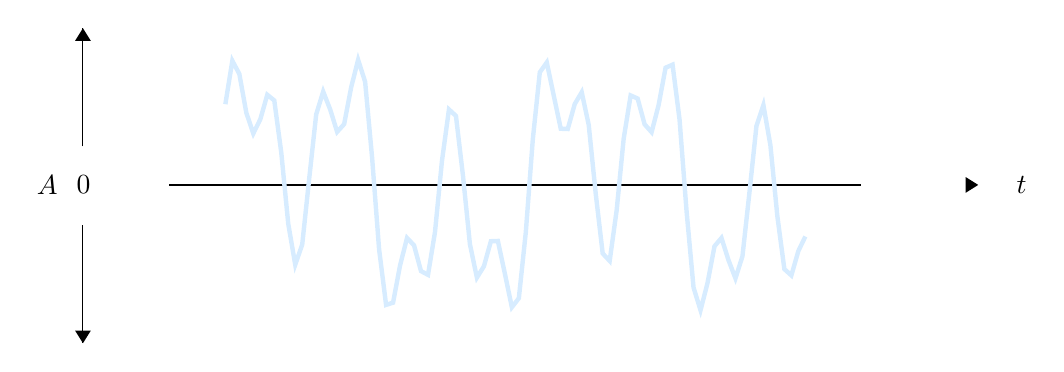
\begin{tikzpicture}
	\begin{axis}[
	width=\textwidth,
	height=5cm,
	tick style={draw=none},
	axis line style={draw=none},
	xticklabels={},
	ytick={0},
	y label style={rotate=270},
	ylabel={$A$},
	domain=-1:13,
	ymin=-5,
	ymax=5,
	]
	\addplot [mark=none, black] {0};
	\addplot [mark=none,
	samples=100,
	textbook-blue-dark,
	ultra thick,
	restrict x to domain=0:12] {2*sin(deg(x))+3*sin(deg(3*x))+2*sin(deg(7*x))};
	\end{axis}
	
	% Update the arrowheads, pls
	\fill (11.15,1.71) -- ++(-0.16,0.1) -- ++(0,-0.2);
	\draw (11.7,1.71) node {$t$};
	
	\draw (-0.22,2.2) -- ++(0,1.5);
	\draw (-0.22,1.2) -- ++(0,-1.5);
	\fill (-0.22,3.7) -- ++(0.1,-0.16) -- ++(-0.2,0);
	\fill (-0.22,-0.3) -- ++(0.1,0.16) -- ++(-0.2,0);
	\end{tikzpicture}
	%}
\end{center}

Analog data are special because they exist in continuous space and thus theoretically have an infinite degree of precision. If we assume a classical model of physics in which time flows continuously, we can model physical quantities with real numbers by writing an equation $A=f(t)$ where $t,A\in\mathbb{R}$. In this sense, a complete set of analog data over a given time interval (i.e. an analog signal) can perfectly describe a physical quantity over the same interval. However, handling analog data can be very difficult. \\

Imagine that you throw a ball in the air and somehow exactly measure its height above the ground at every instant before it lands. If you were to organize these height data with respect to time, you would construct an analog signal that perfectly describes the height of the ball at any point during the throw. In practice, however, no measuring instrument has the required speed or precision necessary to do this. Additionally, you would need an infinite amount of memory to store continuous-time data that is collected at every instant. \\\\

% Need digital data

\begin{tcolorbox}[breakable, enhanced, colback=textbook-blue, sharp corners]
	\vspace{3mm}
	\begin{center}
		\textbf{The Rationale for Binary Numbers}
	\end{center}
	% Implementation details: signals, logic levels, noise, power, reliability
	% Close relationship with classical, two-valued logic
	
	Binary encoding of data is not a requirement for computation. Rather, it is a concession that is made toward digital electronics. Computers have been designed for other bases, and, in some cases, a non-binary encoding is actually preferable. As long as the data can be encoded with a finite number of symbols, it can be handled by a \textit{digital} computer (i.e. a computer that manipulates digits). A digital computer receives and operates on a \textit{discrete} signal of data, a value or set of values that updates at regular time intervals (e.g. every second, every minute, etc.). \\
	
	One could argue that \textit{analog} computers process data that are encoded with an infinite number of symbols. However, this would require a loose definition of "symbol" because analog data cannot be perfectly represented by digits. Rather, analog data is represented in a real, physical medium, like position, pressure, or voltage. An analog computer receives and operates on this \textit{continuous} signal of data that updates instantaneously with real-world time.  \\
	
	Consider the  \hrefcolor[blue]{https://www.youtube.com/watch?v=s1i-dnAH9Y4}{\underline{Mark 1A Fire Control Computer}}, a device, more appropriately termed a "calculator" by modern definitions, that was installed on United States battleships in World War II. This machine used mechanical parts, such as gears, cams, followers, differentials, and integrators, to perform the arithmetic and calculus necessary to hit an enemy ship with a projectile, even if both ships were moving in different directions. It also used smooth components that gradually translated rotational motion into linear motion along a continuum. \\
	
	Despite being labeled with decimal (base-10) integers, this tool actually received \textit{continuous}, \textit{analog} quantities, such as physical position, as input. If each of its mechanical positions were considered a different "symbol," this system would theoretically be able to represent uniquely every real number to a infinite degree of precision and, thus, compute continuous functions without error. Such analog computation is performed also in slide rules, as well as in early electronic computers, which used voltage to represent numbers instead of position. \\
	
	\begin{center}
		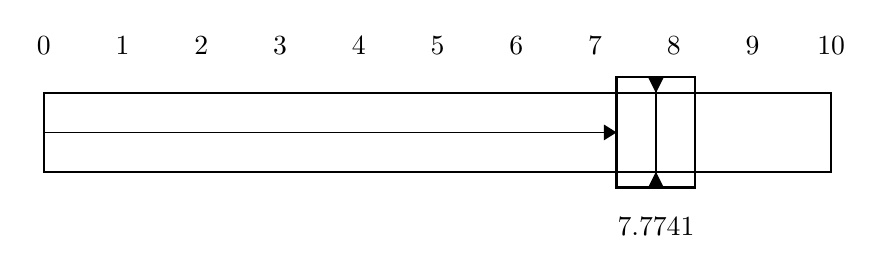
\begin{tikzpicture}
		% Ruler
		\draw [thick] (0,0) rectangle (10,1);
		\draw (0,0.5) -- ++(7.2741,0);
		\fill (7.2741,0.5) -- ++(-0.16,0.1) -- ++(0,-0.2);
		\foreach \i in {0,...,10} {
			\draw (\i,1.6) node {$\i$};
		}
		
		% Slider
		\draw [thick] (7.2741,-0.2) rectangle (8.2741,1.2);
		\draw (7.7741,-0.2) -- (7.7741,1.2);
		\fill (7.7741,0) -- ++(-0.1,-0.2) -- ++(0.2,0);
		\fill (7.7741,1) -- ++(-0.1,0.2) -- ++(0.2,0);
		\draw (7.7741,-0.7) node {$7.7741$};
		\end{tikzpicture}
	\end{center}
	
	% Analog computers have many problems: noise, reproducability
	
	Any digital encoding of numbers is possible in computing, and the choice does not affect what a computer theoretically can or cannot do. Rather, it has practical consequences. Decimal encoding was implemented in a number of early electronic and electro-mechanical computers, such as the Harvard Mark I and the ENIAC. 
	
	% Ternary electronic computers and their issues
	
	% Binary computers and boolean algebra (logic)
	
	% Beyond binary - fuzzy logic (briefly, discuss more deeply later)
	\vspace{3mm}
\end{tcolorbox}
\vspace{2\baselineskip}

% Encoding doesn't have to use numerals. It can use letters, pictures, whatever. You can encode anything anywhere.

% Information signals
% Information systems

Regardless of which encoding is used, data is data.

% All information is encoded and decoded (digital and sensory)

% So, we can represent physical things we experience with digital data. If we collect enough data on the properties of these things, we can simulate reality. We can also simulate abstract mathematical phenomena and other abstract things like language and logic. Much of software design is the simulation of mathematical objects.

% Structured manipulation = algorithm
% The Shannon-Weaver Model of Communication
% Sensory, conversation, and machine examples

% We need to communicate an algorithm in a language
% What kind of language?
% First, let's talk about language in general

% Serialization or marshalling - translating an object (abstract or concrete) into a format that can be stored, communicated, and deserialized into an object again (terms are not quite synonymous in Java)

Data are unorganized facts or statistical values that may reveal something of interest. They are collected by \textit{sampling} the properties of \textit{phenomena} from the observable Universe. Once collected, they can be cleaned, organized, and then analyzed in the hope of gaining a better understanding of reality. When a set of structured data is put into context, it can be interpreted as \textit{information} that explains what has been observed. This information can then be \textit{encoded} as an ordered sequence of data known as a \textit{message}. Messages are \textit{transmitted} and \textit{received} both by Nature and by Man. In the latter case, this process can be viewed as the \textit{communication} of abstract, human thought. \\

Data can describe a variety of things, such as quantities, qualities, and relations. In computer science, data are \textit{quantitative}. That is, they describe \textit{quantities}, which are properties that can be modeled with \textit{numbers}. A quantity can be further classified as either a \textit{multitude} or a \textit{magnitude}. The former is a \textit{discrete} quantity that is \textit{counted}. One would ask "how many" elements belong to a multitude. In contrast, a magnitude is a \textit{continuous} quantity that is \textit{measured}. It is the size of something that is modeled as a \textit{continuum} (e.g. by fields such as $\mathbb{R}$ or $\mathbb{C}$), and one would accordingly inquire as to "how much" of it there is. \\

A set of data collected at a finite rate (e.g. by a \textit{measuring instrument}) is technically a  multitude of samples, even if the quantity being measured is a magnitude. For example, if a ball were thrown in the air, one could ask "how much" height it has at regular intervals of time. Once the data collection ends, one can also ask "how many" samples were acquired. Furthermore, one can ask "how often" samples were taken. This is an evaluation of the \textit{sampling rate}, and it is really just an alternative way of asking with "how much" speed samples were taken. Rates and ratios are still quantities. The existence of the rational numbers $\mathbb{Q}$ are evidence enough of this. \\

Data can be represented by various \textit{media}, both symbolic and physical. In the age of modern computing, data are often assumed to be \textit{digital} in nature, expressed in the symbolic medium of numerical \textit{digits}. This is the case for data processed by modern, electronic computers, which charge capacitors in order to generate voltages that represent \textit{logic levels}. A \textit{transistor} acts as a gate to each capacitor, staying closed to retain \textit{electric charge} during storage and opening to measure or modify voltage on reads and writes respectively. \\

The ratio of a capacitor's charge to its capacitance determines its voltage (i.e. $V=\frac{q}{C}$). This voltage is then mapped to a logic level, which corresponds to a range of voltage values. These logic levels represent digits. In modern computer memory, data are represented as binary digits or \textit{bits} (i.e. the digits 0 and 1), each of which represents a binary number. In this case, there are two logic levels, \textit{low} and \textit{high}. \\

\begin{table}[H]
	\centering
	\caption{Voltage Ranges for CMOS Logic Levels (V)}
	\label{tab:logiclevels}
	\begin{tabular}{|c|c|c|}
		\vtabularspace{3}
		\hline
		Signals & Low (0) & High (1) \\
		\hline
		Input & 0.00--1.50 & 3.50--5.00 \\
		Output & 0.00--0.05 & 4.95--5.00 \\
		\hline
		\vtabularspace{3}
	\end{tabular}
\end{table} 

However, quantitative data need not be expressed with symbolic digits. They can instead be defined in terms of an \textit{analogous} physical quantity. For example, the unit of measurement known as the \textit{millimeter of mercury} (mmHg) defines pressure in terms of the height of a column of mercury in a manometer. It is used to quantify blood pressure, and it does so by considering height an \textit{analog} or \textit{model} of pressure measuring that instead. Using this method, data about one phenomenon can be encoded as data of a different phenomenon, provided that the quantities involved are somehow related to each other. In this case, a height of 1 mm is related to a pressure of 133.322 Pa above atmospheric pressure. \\

% Computation with analog data means you are using actual, original, non-replicable quantites. Computation with digital data means you are using simulated quantities that are replicas or model of what you actually care about. We model EVERYTHING with numbers: physics, language, logic, images, video, music.

% Pros and cons of digital and analog computation

% One can think of digital encoding as a special case of analog encoding, in which a quantity is considered analogous to a sequence of digits that represents a \textit{number}. Because numbers are abstract and data must be concrete, numbers must be associated with symbols known as \textit{numerals} if they are to be used in computation.

%----------------------------------------

\subsection{Semiotics, Language, and Code}

% Types of sentences - declarative and imperative
% An algorithm as an argument

% Computation requires communication
% Model of communication
% All information is encoded and decoded (digital and sensory)

However, the term "universal language" is also often used in other contexts to describe a hypothetical language that all of the world speaks and understands. This is an old idea, and it is addressed in a number of myths and religious texts. In Genesis, the myth of the Tower of Babel explains the diversity of language as a result of God thwarting the Babylonians' plan to build a tower that would extend into the heavens. As punishment for their blasphemy, God "confused their tongues" and dispersed them across the world, shattering their once universal language. Similar myths are told by cultures across the world, such as the Native American Tohono O'odham people, who tell tales of Montezuma attempting to do the same, attracting the ire of the Great Spirit. \\

Alas, no such language exists and it is unlikely that one has ever existed. Rather, human language is generally believed to have evolved independently around the world from prelinguistic systems of communication such as gesturing, touching, and vocalization about 100,000 years ago. Similarly, written language evolved from proto-writing, the repeated use of symbols to identify objects or events. \\

Writing is distinct from speaking in that it is a reliable method of storing and transmitting information. Before the invention of written language, important pieces of history and literature were preserved through \textit{oral tradition}, passing from one generation to the next through repetition and memorization. However, oral tradition is prone to data loss and unintended changes. Like messages in a game of telephone spanning centuries, stories were at risk of losing old details and gaining extraneous ones. Additionally, if a society fell apart, their stories could be lost forever. Writing is a tool that mitigates these issues by \textit{encoding} speech into a symbolic code that can be inscribed onto durable media, such as clay tablets or stone, or onto more delicate, portable media such as parchment or paper. \\

% Quipu, number systems

\begin{tcolorbox}[breakable, enhanced, colback=textbook-blue, sharp corners]
	\vspace{3mm}
	\begin{center}
		\textbf{Symbology in Natural Languages}
	\end{center}
	% Symbol - syntactic, general term
	% Glyphs - syntactic, a graphical representation
	% Characters - semantic, associated with meaning (in computing, it refers to an "encoded character" that is represented by a glyph), a unit of information (which is interpreted by means of a type)
	% Graphemes - the smallest unit in a writing system, a written symbol that represents a sound or phoneme (a logogram, a syllabic character, a letter)
	% Writing systems - ideographic/pictographic systems (Emoji), logographic system, syllabaries, segmental scripts, alphasyllabaries
	% Non-linear alphabets, flag semaphore, animal communication
	% Character encodings
	% ASCII
	% Westernism - Scientific Revolution, alphabet, character, terms and jargon in English (covered in greater detail later)
	% Unicode, code points for abstract characters, UTF-8
	
	A \textit{symbol} is a syntactic mark that is understood to represent a semantic idea. For example, the numeral "$2$" is a symbol for the abstract concept of the number known as "two," the quantity of items in a pair. Symbology is universal for mankind, as it is an exercise of our capacity for abstract thought. Humans can leverage the pattern-recognizing power of the brain to associate symbols or sequences of symbols (also known as \textit{strings}) with ideas. Thus, we can proliferate information textually by means of a \textit{writing system}. \\
	
	Languages are diverse, and so are their writing systems.
	\vspace{3mm}
\end{tcolorbox}
\vspace{2\baselineskip}

% Constructed languages, a subset of which are formal
% Trade language, lingua franca, Latin
% Leibniz - Alphabet of human thought, "best of all possible worlds," panglossianism

An argument of any kind must be expressed in a \textit{language}. In the case of an informal argument, such as a debate, a \textit{natural language} is typically used (i.e. a language, spoken or written, that evolved \textit{naturally} as an aspect of human culture). This is done in the name of \textit{universality}. For example, a political debate that is held and perhaps broadcast in Poland would likely be conducted in Polish because Polish politics are primarily of interest to Polish people. Many Poles speak English in addition to Polish, but there is no language more widely spoken in Poland than Polish, with a whopping 97\% of the country declaring it as their first language. For media directed toward the population of Poland, there is no language that will better ensure an effective dissemination of ideas. It is a nearly \textit{universal} language in this context, a language understood by all intended recipients. \\

Formal proofs, on the other hand, require a \textit{formal language} for clarity and precision. In practice, formal proofs are rarely written or read by logicians or mathematicians. Typically, mathematical proofs are written using a combination of formal and natural language. However, computer programs, written in \textit{programming languages}, are considered formal. \\

A formal language is constructed from an \textit{alphabet} $\Sigma$, which is a set of symbols. The set of all possible finite-length \textit{words} or \textit{formulas} that can be built from this alphabet is denoted $\Sigma^*$. A formal language $L$ over an alphabet $\Sigma$ is then defined as a subset of $\Sigma^*$. Thus, a language is a set of purely syntactic objects. It may conform to a \textit{grammar} that specifies how words can be produced or arranged in a \textit{sentence}, but a language is never inherently meaningful. The semantics of a language is always interpreted separately from the syntax.

% ~~~ Numeral Systems ~~~

% and these numbers can be \textit{encoded} with either a single \textit{symbol} or a sequence of symbols called a \textit{string}. For example, the number eight is typically encoded with the symbol 8, which is a \textit{numeral} or \textit{digit}. The number could just as easily be represented by the symbol \varstigma, but this would be non-standard. Numbers are usually encoded according to an established \textit{numeral system} of some \textit{base} or \textit{radix} that specifies how many unique symbols are used for representation. Numerical data intended to be read by humans are typically encoded in a base-10 system, one of ten digits. \\

% This design choice is ancient and natural. It is based on the ten digits of our hands, which have aided us in counting for hundreds of millennia. In fact, fingers are the oldest counting tools used by man, and we still use them today for this purpose. Other anatomically inspired bases have been used in early numeral systems, such as base-20, which counts the fingers and the toes, or base-12, which uses a thumb on one hand to count the bones of the other four fingers. However, today, the base-10 \textit{Hindu-Arabic numeral system} is universal in mathematics. \\

% The base-60 system of Babylonian numerals is also notable. Its base is thought to have been chosen for its many factors, as this simplifies the process of division. Under this interpretation, this system is \textit{constructed} rather than natural. Instead of mirroring something concrete like physical extremities, this system chooses an abstract base in order to make a procedural optimization. The reasoning for base-2 encoding in computing is similar. It sacrifices human familiarity for performance and reliability. \\

%--------------------------------------------------------------------------------
%    SECTION: LOGIC AND MATHEMATICS
%--------------------------------------------------------------------------------

\toclineskip
\section{Logic and Mathematics}

\vspace{4mm}
\begin{displayquote}
	\textit{Upon this first, and in one sense this sole, rule of reason, that in order to learn you must desire to learn, and in so desiring not be satisfied with what you already incline to think, there follows one corollary which itself deserves to be inscribed upon every wall of the city of philosophy:
	\vspace{1mm}
	\begin{center} Do not block the way of inquiry. \end{center}}
	\vspace{2mm}
	\begin{flushright}
		---Charles Sanders Peirce
	\end{flushright}
\end{displayquote}
\vspace{3mm}

% "Of course, the objects of a deductive system are normally thought of as formulas, the arrows are thought of as proofs or deductions, and operations on arrows are thought of as rules of inference."

% Laws of thought
% Three reliable ways of acquiring information: deduction, induction, and communication.
% Hume's problem of induction
% Deductive: truisms via consequence, Inductive: facts via evidence

% Gottlob Frege
% Alfred Tarski
% Noam Chomsky
% Barbara Partee
% Model-theoretic semantics

%----------------------------------------

\subsection{The Syntax and Semantics of Argument}

\textit{Reasoning} is a cognitive act performed by rational beings. It involves the absorption and synthesis of presently available information for the purpose of elucidating knowledge. It may require the ingenuity of thought, but in some cases the rote application of simple rules is sufficient. Reasoning could also be described as the providing of good \textit{reasons} to explain or justify things. However, as you might expect, there is much debate over whether or not any particular reason is "good." Reasoning is broad, and it comes in different flavors, but ultimately it is the pursuit of \textit{truth}. \\

Reasoning may involve the application of \textit{logic}. This \textit{logical reasoning} is the kind of reasoning that can be expressed in the form of an \textit{argument}. However, this argument does not need to be "correct." Such reasoning simply must be explainable in \textit{steps}, whether that be through informal speech or formal writing. \\

In logic, an argument has two parts: a set of two or more \textit{premises} and a \textit{conclusion}. If the conclusion \textit{necessarily} follows from the premises, the argument is called \textit{valid}. To know whether or not an argument is valid, one must produce a step-by-step \textit{deduction} of the conclusion from its premises. \\

A deduction is constructed within a \textit{deductive system}, which also has two parts: a set of two or more \textit{premises} and a set of \textit{rules of inference}. A rule of inference can be thought of as a kind of logical function. It takes statements (such as premises) as input and outputs either an intermediate result or the conclusion. A deduction, then, has \textit{three} parts: a set of two or more \textit{premises}, a \textit{conclusion}, and a set of \textit{intermediates}. A single-step deduction is represented below, along with a suitable rule of inference labeled $MP$. Note that the set of intermediates is empty in the case of deductions with only one step. \\[2mm]

% Modus Ponens diagram
\begin{center}
	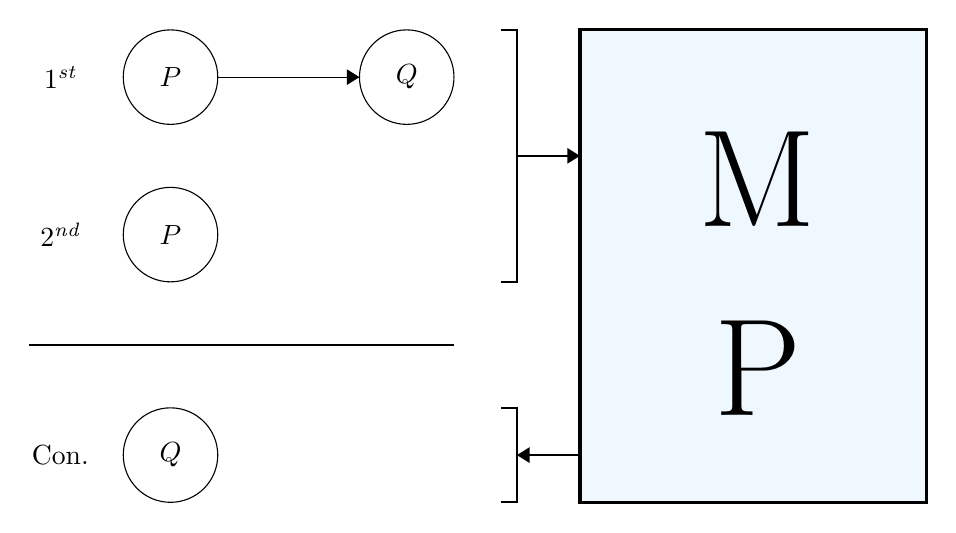
\begin{tikzpicture}[scale=0.2]
	\tikzstyle{every node}+=[inner sep=0pt]
	
	\draw [black] (0,0) circle (3);
	\draw (0,0) node {$P$};
	
	\draw [black] (15,0) circle (3);
	\draw (15,0) node {$Q$};
	
	\draw [black] (3,0) -- (12,0);
	\fill [black] (11.2,0.5) -- (11.2,-0.5) -- (12,0);
	
	\draw [black] (0,-10) circle (3);
	\draw (0,-10) node {$P$};
	
	\draw [black, thick] (-9,-17) -- (18,-17);
	
	\draw [black] (0,-24) circle (3);
	\draw (0,-24) node {$Q$};
	
	\draw (-7,0) node {$1^\textit{st}$};
	\draw (-7,-10) node {$2^\textit{nd}$};
	\draw (-7,-24) node {$\textnormal{Con.}$};
	
	%----------------------------------------
	
	\draw [very thick] (26,3) rectangle (48,-27);
	\fill [textbook-blue] (26.1,2.9) rectangle (47.9,-26.9);
	
	\draw (37,-6.5) node {\fontsize{50}{40} $\textnormal{M}$};
	\draw (37,-18.5) node {\fontsize{50}{40} $\textnormal{P}$};
	
	%----------------------------------------
	
	\draw [black, thick] (22,3.07) -- (22,-13.07);
	\draw [black, thick] (22,3) -- (21,3);
	\draw [black, thick] (22,-13) -- (21,-13);
	\draw [black, thick] (22,-5) -- (26,-5);
	\fill [black] (25.2,-4.5) -- (25.2,-5.5) -- (26,-5);
	
	\draw [black, thick] (22,-20.93) -- (22,-27.07);
	\draw [black, thick] (22,-21) -- (21,-21);
	\draw [black, thick] (22,-27) -- (21,-27);
	\draw [black, thick] (22,-24) -- (26,-24);
	\fill [black] (22,-24) -- (22.8,-23.5) -- (22.8,-24.5);
	\end{tikzpicture}
\end{center}
\vspace{5mm}

This is the quintessential rule of inference used in logical reasoning, expressed here in symbols. It is known as \textit{modus ponens} (Latin for "a method that affirms"). The first premise $P\rightarrow Q$ is called a \textit{conditional statement} where $\rightarrow$ is the \textit{implies} operator. It states that if the \textit{antecedent} $P$ were true, it would \textit{imply} that the \textit{consequent} $Q$ would also be true. The second premise $P$ simply states that the statement $P$ is indeed true. Thus, by means of \textit{modus ponens}, we can \textit{infer} from the premises $P\rightarrow Q$ and $P$ that the conclusion $Q$ must be true. \\

Inference is also called \textit{entailment}. Though these terms describe the same logical concept, the latter more aptly describes the relationship between statements that are connected in a deduction. To infer is to come to a conclusion that is not \textit{explicitly} stated in the premises. To entail is to require that something follows. If $P$ \textit{entails} $Q$, this suggests that $Q$ is a \textit{logical consequence} of $P$, which we can express using a \textit{turnstile}: $P\vdash Q$. Inference is an action that humans perform. Entailment is a relationship between logical rules. \\

When the inferences made mirror the entailment, you've got yourself a \textit{valid} argument. However, this does not necessarily mean that your argument is \textit{sound}. \textit{Validity} is a property of arguments with a conclusion that can be \textit{deduced} from its premises according to rules of inference. However, validity says nothing about whether or not the premises have a \textit{meaning} that accurately describes reality. \textit{Soundness}, on the other hand, is a property of valid arguments whose premises are \textit{known truths} or \textit{axioms}. The deduction of a sound argument is called a \textit{proof}. \\

Validity and soundness complicate entailment. Now, an argument can be evaluated either in terms of its \textit{syntax} or in terms of its \textit{semantics}. Syntax refers to the arrangement of symbolic \textit{words} (or, more generally, \textit{tokens}) in a body of text. Semantics, on the other hand, refers to the \textit{meaning} that can be \textit{interpreted} from the text. Both of these concepts are integral to human language and indeed to the communication of information in general. \\

Consider the following valid deduction: \\

\begin{center}
	\begin{tabular*}{0.55\textwidth}{@{\extracolsep{\fill} } ll}
		\textnormal{"If it is raining, it is Tuesday."} & $P\rightarrow Q$ \\
		\textnormal{"It is raining."} & $P$ \\
		\hline
		\textnormal{"Therefore, it is Tuesday."} & $\therefore Q$ \\
	\end{tabular*}
\end{center}
\vspace{4mm}

This conclusion is a \textit{syntactic consequence} of the premises ($P\vdash Q$). That is, when the argument is evaluated simply as a collection of symbolic strings that are manipulated according to rules, $P$ entails $Q$. \\

Syntactic consequence is sometimes expressed with the following statement: "If the premises are true, the conclusion must also be true." However, while this statement does hold for all valid arguments, text evaluated syntactically does not have any notion of truth. It is simply a sequence of tokens. Thus, it may be better to think of valid arguments as "games that are played according to the rules." For example, chess has no inherent meaning associated with it, but it still has rules, and valid games of chess are those that comply with those rules. \\

Now, it might be Tuesday and raining as you are reading this. However, semantically, it is not required to be Tuesday if it is raining. The first premise given above is, in reality, false. However, if we change it to something that we consider true, we can come to a conclusion that is both valid and sound: \\

\begin{center}
	\begin{tabular*}{0.55\textwidth}{@{\extracolsep{\fill} } ll}
		\textnormal{"If it is raining, it is wet outside."} & $P\rightarrow Q$ \\
		\textnormal{"It is raining."} & $P$ \\
		\hline
		\textnormal{"Therefore, it is wet outside."} & $\therefore Q$ \\
	\end{tabular*}
\end{center}
\vspace{4mm}

In this case, the conclusion is a \textit{semantic consequence} of the premises ($P\vDash Q$). In addition to the argument being syntactically logical, it is also semantically true "in all universes." That is, there is no possible scenario where it is raining, and it is not wet outside. This syntactic-semantic difference will come up repeatedly throughout this guide. \\

%----------------------------------------

\subsection{The Structure of Proof}

Of course, arguments can have more than one step. An argument can involve many inferences, some of which may use \textit{intermediate conclusions} as premises for further conclusions. Multiple threads of reasoning can extend from the premises, weaving through intermediate conclusions and intertwining via inference until they all meet at a \textit{final conclusion}. This is the \textit{tree structure} that is inherent in a \textit{formal proof}. \\

% Tree Structure of Proofs
\begin{center}
	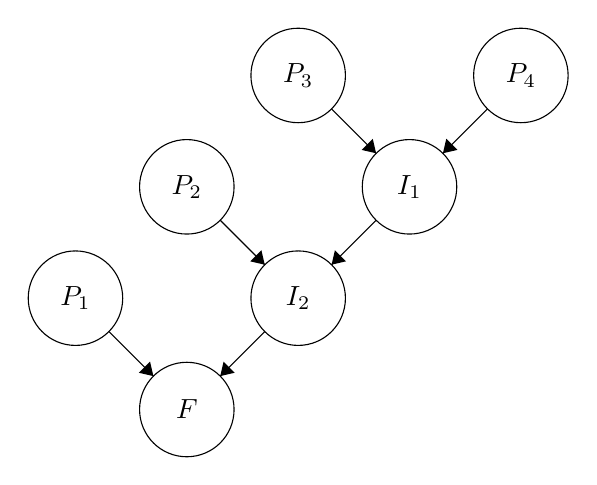
\begin{tikzpicture}[scale=0.2]
	
	\coordinate (L) at (135:10);
	\coordinate (R) at (45:10);
	
	% Level 0
	\draw [black] (0:0) -- ++(L);
	\draw [black] (0:0) -- ++(R);
	
	\fill [white] (0:0) circle (3);
	\draw [black] (0:0) circle (3);
	\draw (0:0) node {$F$};
	
	% Level 1
	\draw [black] (R) -- ++(L);
	\draw [black] (R) -- ++(R);
	
	\fill [white] (L) circle (3);
	\draw [black] (L) circle (3);
	\draw (L) node {$P_1$};
	
	\fill [white] (R) circle (3);
	\draw [black] (R) circle (3);
	\draw (R) node {$I_2$};
	
	% Level 2
	\draw [black] ($ 2*(R) $) -- ++(L);
	\draw [black] ($ 2*(R) $) -- ++(R);
	
	\fill [white] ($ (R) + (L) $) circle (3);
	\draw [black] ($ (R) + (L) $) circle (3);
	\draw ($ (R) + (L) $) node {$P_2$};
	
	\fill [white] ($ 2*(R) $) circle (3);
	\draw [black] ($ 2*(R) $) circle (3);
	\draw ($ 2*(R) $) node {$I_1$};
	
	% Level 3
	\fill [white] ($ 2*(R) + (L) $) circle (3);
	\draw [black] ($ 2*(R) + (L) $) circle (3);
	\draw ($ 2*(R) + (L) $) node {$P_3$};
	
	\fill [white] ($ 3*(R) $) circle (3);
	\draw [black] ($ 3*(R) $) circle (3);
	\draw ($ 3*(R) $) node {$P_4$};
	
	% Arrows	
	\foreach \i in {0,1,2} {
		\coordinate (A) at ($ (45:3) + \i*(R) $);
		\coordinate (B) at ($ (135:3) + \i*(R) $);
		\fill [black,rotate around={45:(A)}] (A) -- ++(0.8,0.5) -- ++(0,-1);
		\fill [black,rotate around={45:(B)}] (B) -- ++(-0.5,0.8) -- ++(1,0);
	}
	
	\end{tikzpicture}
\end{center}
\vspace{4mm}

In this \textit{tree}, the \textit{first premises} are labeled as $P_n$ where $n\in\{1,2,3,4\}$, the \textit{intermediate conclusions} are labeled as $I_m$ where $m\in\{1,2\}$, and the \textit{final conclusion} is labeled $F$. Though one can make a distinction between first premises and intermediate conclusions, it is important to note that they are all premises with regard to the eventual final conclusion. Thus, there are no restrictions on combining them beyond those dictated by the rules of inference. \\

In modern proof theory, proofs like these are studied not only for their semantic meaning, but also for their mathematical structure. They are treated like \textit{data structures}, which are abstract objects that are used in computer science to model the storage and flow of digital \textit{information}. Similarly, a proof is an abstract text that models the flow of logical information as it is manipulated by rules of inference toward a final conclusion. \\

Information, in the context of computer science and, more generally, \textit{information theory}, refers to a \textit{syntactic} message. Formally, it is an order sequence of symbols \\

% Data

In computer science, the data structures of interest are \textit{recursive}. That is, the structure can be defined "in terms of itself." \textit{Recursion} is a deep topic, and we will spend much of the next part characterizing it, but a practical way to think about a recursive structure is in terms of \textit{type}. \\

Types are a widespread feature in programming languages. As a concept, they are founded in a logical system called a \textit{type theory}. There are multiple type theories, and some of them are used as alternative foundations for mathematics. We will cover all of this in detail later, but, essentially, a type is a label that can be given to 

% Proofs and models
% String together arguments to make proofs
% Tree structure of arguments
% List structure of arguments
% Data structures structure data in such a way that it can be interpreted as a model of semantic ideas.
% Proofs structure text in such a way that...
% Information is syntactic, data is semantic

However, not all forms of reasoning have such strict rules. There are other methods of reasoning that cannot be modeled by an argument. In contrast to logical reasoning, \textit{intuitive reasoning} has steps that are \textit{not} understood. Although the question might seem peculiar, it is worth asking whether or not computation can be intuitive. So, to begin our journey of understanding computation in a modern, logical sense, we will first walk in the other direction, considering it instead in a mystical, otherworldly sense. \\

%----------------------------------------

\subsection{The Oracle, the Seer, and the Sage}

\textit{Intuition} is the capacity to create conclusions without evidence, proof, or a combination of the two. If any premises are involved, they may appear to an onlooker as if they were plucked out of thin air. If any method is involved, it is esoteric or hidden from sight. Acts of intuition range from the mundane procedures we perform without thinking to great feats of intellectual, artistic, and athletic achievement. And while it is often associated with magic or supernatural ability, intuition is a real, observable phenomenon, and it is a form of reasoning. \\

Like that of reasoning, the definition of intuition is fuzzy. There are a variety of events that one might label as the product of intuition that are actually quite functionally distinct from one another. For this reason, I would like to consider and compare three archetypes that are known for their intuitive skills: the Oracle, the Seer, and the Sage. For the skeptics among you, I ask that you suspend your disbelief for a moment and assume that our characters are acting in good faith. There is no lying here; the conclusions are sincere. \\

\paragraph{The Oracle} \hspace*{1mm} \vspace*{2mm}

An Oracle is a person who predicts the future by acting as a vessel for a god or a set of gods. They are considered by believers to be portals through which the divine speaks directly. They are found in histories all over the world, but most people associate the role with the priestesses of Ancient Greece. Picture a woman with eyes that roll back into her head as she speaks in a possessed, thundering voice. \\

For an Oracle, the conclusions come straight from the source. She may not even do any reasoning herself, save for the \textit{unconscious reasoning} that is performed while she is possessed. However, conscious or not, she provides a great service to mankind. There is no clearer answer than the one given to you directly from the gods themselves, even if it has to be sent through what is essentially the human version of a telephone. \\

For those seeking counsel, the premises of the Oracle's conclusion are unnecessary because they just \textit{know} that the statement must be true. For them, the connection the Oracle has with the gods and with reality is part of life itself. We all have deep beliefs like this. For example, most people do not feel that gravity needs to be proven to them in order for them to accept it as fact. Their perception of gravity in the world around them is proof enough. This is the kind of intuition characterized by \textit{subconscious reasoning}, the reasoning you do without being aware of doing it. \\

\paragraph{The Seer} \hspace*{1mm} \vspace*{2mm}

A Seer is a person who predicts the future by interpreting signs from a god or a set of gods. Unlike an Oracle, a Seer speaks divine truth in his own words, drawing from an innate, sometimes god-given power to see meaning in natural events or occult objects. There are various methods of divination that are used by Seers, such as scrying (the gazing into magical things, like crystal balls, for the purpose of seeing visions), auspicy (the interpretation of bird migration), or dowsing (the use of magic to find water, often with the aid of a dowsing rod). The acceptance of any particular method is cultural, but beliefs in divination vary greatly, even within a single society. \\

The Seer has premises for his conclusion, but the rules of inference involved in his reasoning are incomprehensible to others. He 

\paragraph{The Sage} \hspace*{1mm} \vspace*{2mm}

% Seers have premises and conclusions, oracles just speak conclusions
% Does intuition involve unconcious, preconcious, or concious reasoning?
% Is intuition computation?
% This book is as much about intuition as it is about computation.
% In some sense, intuition is thought of as the opposite of logic (it has no argument or basis in reality)
% In another sense, logical truths (tautologies) could be considered intuitive, so all of logic could be the product of intuition. Unless you believe that logic is objective.
% The Oracle and the Seer are unique from the sage because they KNOW their truth is absolute.
% Computers are honestly closer to oracles or seers than sages.
% Buddhism - intuition is a faculty of the mind of immediate knowledge

\begin{tcolorbox}[breakable, enhanced, colback=textbook-blue, sharp corners]
	\vspace{3mm}
	\begin{center}
		\textbf{What is Truth?}
	\end{center}
	Truth, in the absolute sense, has been discussed and debated since the dawn of man. It is a concept that seems obvious to us, and yet it always seems to elude our understanding. Philosophers have formulated dozens of theories of truth over the years, with some asserting that truth is an objective property of our universe and others asserting that truth is a useful lie that mankind has invented. And while there is merit in those claims that truth is not real, we still see around us the technology that was born out of our intuitive sense of true and false. Especially in computer science where everything is represented in binary. \\
	
	The traditional theories of truth have been termed \textit{substantive}. That is, they assert that truth has some basis in reality and that it is a meaningful thing to discuss. Early theories of truth from Ancient Greece are considered the foundation of \textit{correspondence theory}, the idea that statements are true if their symbols are arranged in such a way that they express an abstract thought that accurately describes reality. This theory defines truth in the context of a relationship between language and objective reality. It is a useful philosophy that allows us to orient ourselves in the world around us. However, many philosophers believe that truth cannot be explained by such a simple rule. In fact, there are many more factors that could play a role in the concept. \\
	
	Objections to a strict correspondence theory usually take issue with the treatment of language as something monolithic and easy to classify within a true-false dichotomy. For example, a statement encoded as a sentence in a language is only meaningful to people who can read that language. What does this imply about a particular language's relationship with truth? Is a statement only true for those who understand it? Furthermore, there is no guarantee that readers of the same language will even be able to agree on the meaning expressed by a particular sentence. Languages often encompass multiple dialects that might parse words differently. Words themselves also may not be precise, and some abstract thoughts may not have suitable words in some languages. These are the points raised in \textit{social constructivism}, a theory which avers that human knowledge is historically and culturally specific. Social constructivists also believe that truth is \textit{constructed} and that language cannot faithfully represent any kind of objective reality. \\
	
	Other substantive theories find the essence of truth nestled in other abstract concepts. \textit{Consensus theory}, as the name implies, defines truth as something that is agreed upon either by all human beings or by a subset (such as academic groups or standards bodies). This is another anthropocentric definition that is at constant risk of philosophical division on any given topic. \textit{Coherence theory} takes a more objective approach, claiming that a statement can only be true if it fits into a system of statements that support each other's truth. This is similar to the notion of \textit{formal systems}, which we will discuss in depth later. However, traditional coherence theories attempt to explain all of reality within a single coherent system of truths, which is incompatible with our modern understanding of formal systems. \\
	
	Modern developments in philosophy have resulted in theories that deviate from the long-held, substantive opinions on the nature of truth. These \textit{minimalist} theories assert instead that truth is either not real or not a necessary property of language or logic. They claim that statements are \textit{assertions} and thus are implicitly understood to be true. For example, it is understood that by putting forth the sentence "$2+2=4$," you are endorsing the semantic meaning "$2+2=4$ is true." The clause "is true" is called a \textit{truth predicate}, and minimalist theories of truth often consider its use redundant. \\
	
	This idea of a truth predicate is borrowed from Alfred Tarski's \textit{semantic theory of truth}, which is a substantive theory that refines the correspondence concepts espoused by Socrates, Plato, and Aristotle for formal languages. This theory makes a distinction between a statement made in a formal language and a truth predicate, which evaluates the truth of the statement. Tarski made this distinction in order to circumvent the \textit{liar's paradox}, which is often presented with the following example: "This sentence is false." If the predicate "is false" is considered to be part of "this sentence," the truth of this statement cannot be decided. For this reason, Tarski states that a language cannot contain its own truth predicate. This is enforced by requiring that "this sentence" be written in an \textit{object language} and that "is false" be written in a \textit{metalanguage}. \textit{Convention T}, the general form of this rule, can be expressed as
	
	\begin{center}
		\textit{"$P$" is true if and only if $P$}
	\end{center}
	
	where "$P$" is simply the metalanguage sentence $P$ rendered in the object language. That is, the \textit{syntactic representation} is assigned a \textit{truth value} of true if and only if the semantic meaning it represents is considered true (according to whatever theory of truth you employ). By this rule, we say that "$2+2=4$" is true if and only if \textit{the sum of the number $2$ with the number $2$ is equal to the number $4$}. Minimalist redundancy theories modify Tarski's theory by interpreting "$P$" as an implicit assertion of the truth of $P$. The sentence "$P$," which asserts that $P$ is true, is then false if and only if its semantic meaning $P$ is false. \\
	
	\parbreak
	
	The debate on the nature of truth rages on \textit{in perpetuum}. However, for our purposes, we must be practical. There is truth in logic and mathematics and computer science as well, but, in practice, it has little to do with the debates on \textit{absolute truth} described above. Their truth is \textit{relative}. That is, it relies on the assumption that our premises are true. Cognizant of this, we move forward with our thinking, searching for truths within these arbitrary boundaries. \\
	\vspace{3mm}
\end{tcolorbox}
\vspace{2\baselineskip}

%----------------------------------------

\subsection{The Mathematician and the Scientist}

% Deductive and Inductive (+ Abductive)
% Mathematician write proofs (deductive), but they also use creativity (inductive)
% Is creativity inductive?
% Human computer

Logical reasoning is the \textit{inference} of new information from present information. It involves \textit{rule of inferences} that are used to relate sets of \textit{premises} to \textit{conclusions}. There are three kinds of logical reasoning: \textit{deductive}, \textit{inductive}, and \textit{abductive}. Each is classified according to which piece of information (premises, rule, or conclusion) is missing and must be inferred from the others. \\

% Explanatory vs ampliative
% Certainty vs uncertainty (probability)
% Top-down vs bottom-up
% Logical truths (tautologies) vs facts
% Abduction = induction + justification
% Closed and open world assumptions
% Domain of discourse

Inductive arguments exist on a spectrum between \textit{weak} and \textit{strong}. Those that are stronger and more persuasive have a higher probability of having a true conclusion. Inductive reasoning is associated with \textit{science} and \textit{critical thinking} because it allows one to make generalizations about complex phenomena given limited evidence. Unlike deductive reasoning, it attempts to find new knowledge that is not simply contained within its premises. \\

Statements made by induction are bolstered with evidence whereas deductive statements are as true as their premises. This leaves inductive reasoning susceptible to \textit{faulty generalizations} and \textit{biased sampling}. Induction must also assume that future events will occur exactly as they have in the past, which is not always the case. For example, a turkey that is fed every morning with the ring of a bell may infer by induction that bell $\rightarrow$ food. However, he will see the error in his reasoning when the farmer rings the bell on Thanksgiving Day and instead slits his throat. \\

\paragraph{Abductive Reasoning} \hspace*{1mm} \vspace*{2mm}

\textit{Abductive reasoning} is the inference of a \textit{premise}, given a conclusion and a rule. It is investigative in nature. For example, given a conclusion "The grass is wet" and a rule "When it rains, the grass gets wet," we might determine that rain is the best explanation for the wetness of the grass. Thus, we abduce that "It might have rained." \\

Like induction, abduction can also produce a hypothesis. However, abduction does not seek a new relationship between two previously unconnected statements. Rather, it uses established relationships to find a reasonable explanation for a statement that is assumed to be true. It is often used by detectives or diagnosticians who need to find a probable cause of an event. It is also used in Bayesian statistics. While multiple premises may be abduced, typically we want to abduce a single, "best" premise. \\

Abductive reasoning allows us to ignore the many causes that are unlikely in favor of those few that may be relevant to the problem at hand. For example, doctors are often taught to heed the following proverb: "When you hear hoofbeats, think of horses, not zebras." That is, when a patient exhibits certain symptoms, a doctor should abduce from them a commonplace disease before considering more exotic possibilities. However, "zebras" do exist. Sometimes the most likely cause is not the actual cause. For this reason, abduction is also considered to be equivalent to a deductive fallacy called \textit{affirming the consequent}, which is like a \textit{modus ponens} performed in reverse. That is, given a conditional $P\rightarrow Q$ and the consequent $Q$, abduction infers $P$ from $Q$ by assuming that the converse $Q\rightarrow P$ of the conditional is also true. This is not a deductively valid inference. Considering our example again, the grass might be wet from rain, but this is not \textit{necessarily} true. It is also possible that the sprinkler system is on. Or perhaps there is a zebra-esque scenario like a flood. \\\\

%-------

\begin{tcolorbox}[breakable, enhanced, colback=textbook-blue, sharp corners]
	\vspace{3mm}
	\begin{center}
		\textbf{Induction and Abduction}
	\end{center}
	% Can computers induce?
	% Machine learning simulates induction deductively
	% Deductive computers, AI, General AI, Artificial Conciousness
	% Calculation vs Computation
	
	% Fuzzy expert systems "abduce"
	TEXT
	\vspace{3mm}
\end{tcolorbox}
\vspace{2\baselineskip}

%----------------------------------------

\subsection{Mechanical Computation}

% Computation done by humans mechanically with tools
% Computation done entirely by machines

Before we discuss and classify automata in depth, we should first consider what is \textbf{not} an automaton. What is an example of something that might perform some kind of calculation, but is not a computer? What about a microwave? Is a microwave a computer? No, it is not. A computer can be programmed in some meaningful, robust way. A microwave contains a microprocessor, which uses \textit{combinational logic} and basic binary inputs to set timers and operate the oven. It cannot be programmed in any meaningful way. What about a calculator? Is a calculator a computer? If we are being formal, the answer is no, but it depends on what kind of "calculator" we are talking about. \\

Calculators, such as \textit{counting boards} and the \textit{abacus}, have been around since pre-history. Calculators with four-function capabilities have been around since the invention of Wilhelm Schickard's mechanical calculator in 1642. In the late 19th century, the \textit{arithmometer} and comptometers, two kinds of digital, mechanical calculator, were being used in offices. The Dalton Adding Machine introduced buttons to the calculator in 1902, and pocket mechanical calculators became widespread in 1948 with the \textit{Curta}. None of these are computers. \\

The difference between a calculator and a computer is that a computer can be programmed and a calculator cannot. What does it mean to be programmable? That is perhaps the central question of automata theory, and we will discuss in this section several levels of "programmability." However, for now, we can certainly say that a simple, four-function electronic calculator is not a computer. It simply uses combinational circuits like full-adders, full-subtractors, multipliers, and dividers to implement its functions, and there is no potential for modifications or user-defined functions. \\

Surprisingly enough, \textit{special-purpose computers} have also been around for a long time. Early examples include the \textit{Antikythera mechanism} (an Ancient Greek analog computer), Al-Jazari's 1206 water-powered \textit{astronomical clock}, the 1774 \hrefcolor[blue]{https://www.youtube.com/watch?v=bY\_wfKVjuJM}{\underline{Writer Automaton}} (a mechanical doll that could be programmed to write messages), the 1801 \textit{Jacquard loom}, and \textit{slide rules}. Some later mechanical computers were quite powerful, such as \textit{differential analyzers} (special-purpose computers for solving differential equations) and fire control computers. Charles Babbage designed the \textit{Analytical Engine}, a general-purpose computer, in 1837, and Ada Lovelace wrote a program for it, but it was never built. General-purpose computing would not reemerge until the 1940s. \\

The line between calculator and computer began to blur with the introduction of \textit{programmable calculators} in the 1960s. Many modern high-end calculators are programmable in Turing-complete languages such as TI-BASIC or even C or C++, which officially makes them computers. Once we start implementing \textit{sequential logic} with components like SR latches or D flip-flops, we are storing state, and state is a requirement for computing. Circuits that use sequential logic can be considered automata and, given enough complexity, computers. \\\\

\begin{tcolorbox}[breakable, enhanced, colback=textbook-blue, sharp corners]
	\vspace{3mm}
	\begin{center}
		\textbf{Modern Computing is American}
	\end{center}
	TEXT
	\vspace{3mm}
\end{tcolorbox}
\vspace{2\baselineskip}

Blah \\

% Hey, let's build machines to do this instead.
% Wait, what exactly are we building? Let's model the problem.
% Computation as a mechanical process vs a function.
% Abstract away the mechanics, and a function becomes a conversation (input and output).
% Computing is more than just math, semantically.
% Structure of language, types of sentences (declarative/imperative)

\parbreak

What is the strange loop? What is wisdom?

% \textbf{Wisdom} is the capacity to think and act in a way that is right. It involves the use of knowledge, a prudent choice of means and ends, and a healthy doubt of one's own understanding. It is born of an acknowledgment of how little one truly knows and how little control one truly has. \\

% The wise exhibit:
% Realism
% Gratitude
% Understanding of folly
% Humor
% Politeness
% Self-acceptance
% Forgiveness
% Resilience
% Control over envy
% Little regret
% Calmness
 % Philosophy of Computation
%--------------------------------------------------------------------------------
%--------------------------------------------------------------------------------
%    CHAPTER II: THEORY OF COMPUTATION
%--------------------------------------------------------------------------------
%--------------------------------------------------------------------------------

\part*{Theory of Computation}
\addcontentsline{toc}{part}{\tocpartglyph Theory of Computation}

\vspace{\baselineskip}
\begin{displayquote}
	\textit{Theory is relevant to you because it shows you a new, simpler, and more elegant side of computers, which we normally consider to be complicated machines. The best computer designs and applications are conceived with elegance in mind. A theoretical course can heighten your aesthetic sense and help you build more beautiful systems.}
	\begin{flushright}
		---Michael Sipser
	\end{flushright}
\end{displayquote}
\vspace{4mm}

% Mathematical modeling of computation (sequential, functional, concurrent)
% Automata theory covers sequential and concurrent, computability theory covers functional. Together, they cover the prominent models of computations.
% Computational complexity theory is a categorization of computational tasks.

The \textit{theory of computation} is a field of study that is related to both mathematics and computer science. It is concerned with a process known as \textit{computation}, which refers to any kind of \textit{calculation} (the transformation of one or more inputs into one or more outputs) that is accomplished by following an \textit{algorithm} (a set of rigorously defined steps). It is also concerned with the formalization of theoretical models of computation known as \textit{abstract machines} or \textit{abstract automata}. Also of interest are the \textit{computational problems} that can be solved by these abstract machines and how efficiently they can be solved. The theory of computation gives us the formal definition of a computer and the scope of what a computer can accomplish. \\

Much of the work in the theory of computation is$\dots$ quite abstract. While calculation and computation have been practiced by humans for thousands of years, the concept was only formalized by mathematicians, logicians, philosophers, linguists, and computer scientists in the past 150 years. This part of the guide will delve into some fairly academic topics with a decent amount of mathematical rigor, but it is written to be accessible and entertaining. \\

The field has three branches: \textit{automata theory}, \textit{computability theory}, and \textit{computational complexity theory}, each of which asks fundamental questions pertaining to how mathematical calculations can be automated, which kinds of problems can be solved by a machine, and how many resources are required to solve a particular problem. We will touch on the major discoveries made in each of these branches and discuss why they are significant to computer science and programming in general.

% "Graduate-level mathematics"

%--------------------------------------------------------------------------------
%    SECTION: AUTOMATA THEORY
%--------------------------------------------------------------------------------

\toclineskip
\section{Automata Theory}

% Concept of automata
% Models of computation
% Computation requires state, transition, and language

\textit{Automata theory} is the study of \textit{automata} and their behavior. An \textit{automaton} is a self-operating machine designed to follow or respond to a predetermined sequence of operations. Automata include physical devices such as cuckoo clocks, mechanical watches, robots, and computer processors as well as \textit{abstract machines}. An abstract machine is any formal description of \textit{mechanical behavior}. An abstract machine that is used to formally describe computation is called a \textit{model of computation}. This is a mathematical description of what a computer is, and it models the computation that a real, concrete computer could actually perform, if you were to implement that computer according to the model's specifications. Like their concrete counterparts, abstract machines have \textit{state}, a set of information in the \textit{present} that was acquired due to \textit{past} events. All automata begin with a \textit{starting state}, receive some sort of \textit{input}, and \textit{transition} to another state based on the value of that input and the value of its current state. \\

One \textit{abstract automaton} in particular fully models not only the computation that is performed by today's state-of-the-art computers, but also the very process of computation itself. We will spend a lot of time in this guide discussing the structure and behavior of this model as well as what its limitations imply regarding the future of computing, software, mathematics, and the meaning of life. We will also briefly explore the abstract automata that exist in pure mathematics and model computation that is not physically realizable. \\

%----------------------------------------

\subsection{From Knots to Nodes}

% Explain what graphs are so you can use them to model automata.

It is worth pausing here to think about what the word \textit{node} really means. It comes from the Latin word \textit{nodus}, which means \textit{knot}. A node is like a knot in a string: a distinguishable lump at a certain position. And between any two adjacent knots in a string, there is a \textit{link} \dots\ of string. Similarly, between any two adjacent links, there is a knot. \\

The knots and the links cannot exist independent of each other. Without knots, there are no links of string---just one, continuous string. Without links, knots are totally unanchored and have no sense of position. Now, one could argue that a single knot is sufficient for the existence of links in a string, but such a view is naive and presumes a familiar, everyday sort of string. \\

For example, yes, you can tie a single knot in a shoelace, and you might then call the floppy bits on either side of it "links." But when you call something like this a link, what you are really pointing out is its \textit{finite length}. That is, the "string link" \textit{starts} at the knot and \textit{ends} at the tip of the aglet. But length is a nonessential detail for links---the essence of a \textit{link} is its \textit{connecting} of things. A better term in this case would be \textit{loose end} or simply \textit{end}. A knot with two loose ends is shown below: \\

\begin{center}	
	\begin{tikzpicture}[scale=0.2]
	\begin{knot}[
	consider self intersections,
	flip crossing=2
	clip width=5,
	]
	\strand[ultra thick]
	(90:1.25) to[out=180,in=-120,looseness=2]
	(-30:1.25) to[out=60,in=120,looseness=2]
	(210:1.25) to[out=-60,in=0,looseness=2] (90:1.25);
	\end{knot}
	
	\draw [ultra thick, dashed] (-1.2,0) -- ++(-5,0);
	\draw [ultra thick, dashed] (1.2,0) -- ++(5,0);
	\end{tikzpicture}
\end{center}

For our purposes, it is better to envision a taut string that stretches to infinity in both directions and to think of a \textit{link} as a \textit{connector of a knot pair} whose length may or may not be important. With this model, there must be at least two knots in the string if we are to think of them as \textit{nodes} (i.e. things that are connected to something else). A string with five \textit{trefoil} (three-leafed) knots and four links is shown below: \\

\begin{center}
	\begin{tikzpicture}[scale=0.2]
	\foreach \x in {-2,-1,0,1,2} {
		\begin{knot}[
		consider self intersections,
		flip crossing=2
		clip width=5,
		xshift=\x*250,
		]
		\strand[ultra thick]
		(90:1.25) to[out=180,in=-120,looseness=2]
		(-30:1.25) to[out=60,in=120,looseness=2]
		(210:1.25) to[out=-60,in=0,looseness=2] (90:1.25);
		\end{knot}
	}
	
	\foreach \x in {-1,0,1,2} {
		\draw [ultra thick] (-1.2+\x*8.75,0) -- ++(-6.45,0);
	}
	\draw [ultra thick, dashed] (-18.75,0) -- ++(-9,0);
	\draw [ultra thick, dashed] (18.75,0) -- ++(9,0);
	\end{tikzpicture}
\end{center}

In the mathematical field of \textit{knot theory}, knots are defined similarly, but they do not have ends. That is, a mathematical knot is defined as a \textit{closed} circle embedded in a three-dimensional Euclidean space and subject to continuous deformation. Essentially, this means that you can cut a circular string at a point, tangle it, and close the circle at the same point to form any mathematical knot you like. The process of tying a \textit{cinquefoil}, a knot with five \textit{crossings}, is given below as an example: \\[\baselineskip]

\resizebox{\textwidth}{!}{
	\begin{tikzpicture}
	\draw[very thick] (0,0) circle (2);
	\filldraw[line width=1mm,textbook-blue] (0,0) ++(60:2) arc (60:70:2);
	
	\begin{knot}[
	consider self intersections,
	flip crossing=2
	clip width=5,
	xshift=150
	]
	\strand[very thick] (2,0) .. controls +(0,1.0) and +(54:1.0) .. (144:2) .. controls +(54:-1.0) and +(18:-1.0) .. (-72:2) .. controls +(18:1.0) and +(162:-1.0) .. (72:2);
	\end{knot}
	
	\begin{knot}[
	consider self intersections=true,
	%  draft mode=crossings,
	flip crossing/.list={2,4},
	only when rendering/.style={
		%    show curve controls
	},
	xshift=300
	]
	\strand[very thick] (2,0) .. controls +(0,1.0) and +(54:1.0) .. (144:2) .. controls +(54:-1.0) and +(18:-1.0) .. (-72:2) .. controls +(18:1.0) and +(162:-1.0) .. (72:2) .. controls +(162:1.0) and +(126:1.0) .. (-144:2);
	\end{knot}
	
	\begin{knot}[
	consider self intersections=true,
	%  draft mode=crossings,
	flip crossing/.list={2,4},
	only when rendering/.style={
		%    show curve controls
	},
	xshift=450
	]
	\strand[very thick] (2,0) .. controls +(0,1.0) and +(54:1.0) .. (144:2) .. controls +(54:-1.0) and +(18:-1.0) .. (-72:2) .. controls +(18:1.0) and +(162:-1.0) .. (72:2) .. controls +(162:1.0) and +(126:1.0) .. (-144:2) .. controls +(126:-1.0) and +(0,-1.0) .. (2,0);
	\end{knot}
	\end{tikzpicture}
} \\[\baselineskip]

% There are no ends for each knot. A single knot is closed. Links are not like above.

Note that because mathematical knots are closed, they cannot be linked together like knots in a string. Instead, a link in knot theory is a collection of knots that are knotted together. \\

% We, however, are interested in the more general \textit{graph theory}, whose focus is on how knots are connected to other knots rather than on the structures of the knots themselves. A \textit{graph} is a drawing of objects and relations in which each object or \textit{node} is represented by a circle and each relation or \textit{link} is represented by a line or arrow. \\

% The string above can be thought of as a list. Here are some other structures that are graphs (tree, grid, two linked knots)

% Node is a joint or a communication hub in an information system. It is connected to other nodes by links or communication channels. Node is Latin for knot. So node/connection in information science, vertex/edge in graph theory.

% Calculation vs computation. Separate histories.
% Is a microwave a computer?
% Modern cars are full of computers. Embedded systems.

%----------------------------------------

\subsection{Exploring the Link Between Concrete and Abstract Machines}

Let's take a simple, concrete machine and try to visualize the abstract machine that underlies it. Consider a cuckoo clock. Every day, at noon, a small plank with a mechanical bird perched on its lip will extend from a hole above the clock face, powered by a working motor. Once the plank is fully extended, the bird will flap its metal wings and maybe turn its head as a song is played from a revolving music box inside the clock. Then, when it is 12:01 PM, the music will stop, the bird will still, and the plank will retract. The process will occur again the next day, at noon. \\

The machine's components here are the plank, the bird, and the music box. The components each have two states: the plank can be retracted or extended, the bird can be still or flapping its wings, and the music box can be paused or playing. The input to this machine is whether or not the clock hands both point straight at 12. We can say that this automaton has a state that can be expressed in terms of the states of its components. We can represent its starting state with the sequence (0,0,0) (i.e. the plank is retracted, the bird is still, and the music box is paused). The automaton can receive one of two inputs, 1 or 0 (i.e. both clock hands point straight at 12 or they do not). This input might be implemented with an electromechanical switch that turns the motor on or off.

\paragraph{(0,0,0) -> (1,0,0)} We start at state (0,0,0). As the morning passes, the automaton receives a constant input of 0, which keeps it in its starting state. At noon, the input switches to 1, and the automaton transitions to the state (1,0,0). As the plank extends and transitions its own state from 0 to 1, the bird remains still, and the music box remains paused. Once the plank is fully extended, we are in state (1,0,0).

\paragraph{(1,0,0) -> (1,1,1)} We expect that the plank will be fully extended well before 12:01 PM, so the input should still be 1. However, if for some reason the input is 0, we should transition back to (0,0,0), as the machine should only operate outside of its starting state between 12:00 and 12:01 PM. This is a simple example of \textit{strange input}. The input 0 at this state is unexpected, but it is technically possible. It is a better idea to define the behavior for this unexpected case, rather than to allow the input to cause unexpected behavior. On the other hand, if the input is 1 at this state, the automaton transitions to the state (1,1,1). The plank is fully extended, the bird is flapping its wings, and the music box is playing.

\paragraph{(1,1,1) -> (0,0,0)} Before 12:01 PM, the input is still 1, and that input should keep the automaton in its current state of (1,1,1). When 12:01 PM rolls around, the input will now be 0. In this case, we would like to return to the original state. On receipt of the input 0 while in state (1,1,1), the automaton transitions back to its starting state, (0,0,0). This abstract machine is shown below with a state format of (plank, bird, music) and an input specifying if the clock hands point exactly toward 12.

% Drawing of "Bad Automaton"
\begin{center}
	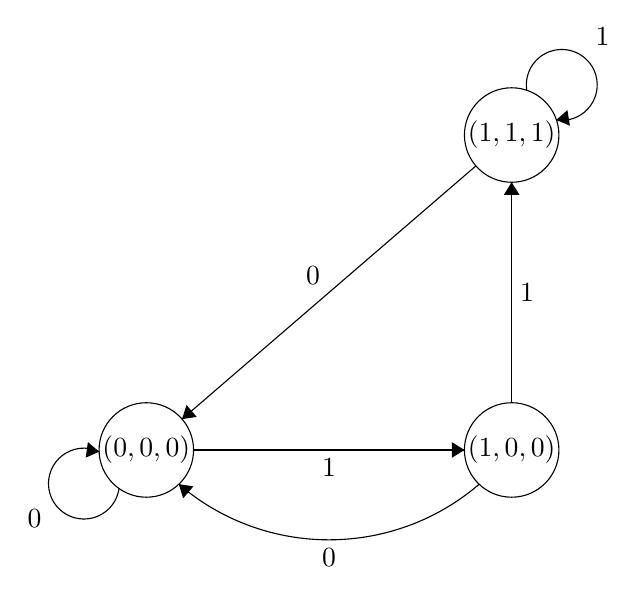
\begin{tikzpicture}[scale=0.2]
	\tikzstyle{every node}+=[inner sep=0pt]
	\draw [black] (28.4,-36.5) circle (3);
	\draw (28.4,-36.5) node {$(0,0,0)$};
	\draw [black] (51.6,-36.5) circle (3);
	\draw (51.6,-36.5) node {$(1,0,0)$};
	\draw [black] (51.6,-16.5) circle (3);
	\draw (51.6,-16.5) node {$(1,1,1)$};
	\draw [black] (31.4,-36.5) -- (48.6,-36.5);
	\fill [black] (48.6,-36.5) -- (47.8,-36) -- (47.8,-37);
	\draw (40,-37) node [below] {$1$};
	\draw [black] (51.6,-33.5) -- (51.6,-19.5);
	\fill [black] (51.6,-19.5) -- (51.1,-20.3) -- (52.1,-20.3);
	\draw (52.1,-26.5) node [right] {$1$};
	\draw [black] (26.668,-38.935) arc (-7.69924:-295.69924:2.25);
	\draw (21.78,-40.87) node [left] {$0$};
	\fill [black] (25.41,-36.61) -- (24.69,-36) -- (24.55,-36.99);
	\draw [black] (49.539,-38.673) arc (-49.35642:-130.64358:14.645);
	\fill [black] (30.46,-38.67) -- (30.74,-39.57) -- (31.39,-38.81);
	\draw (40,-42.71) node [below] {$0$};
	\draw [black] (52.56,-13.67) arc (189:-99:2.25);
	\draw (56.9,-10.25) node [right] {$1$};
	\fill [black] (54.43,-15.54) -- (55.3,-15.91) -- (55.14,-14.92);
	\draw [black] (49.33,-18.46) -- (30.67,-34.54);
	\fill [black] (30.67,-34.54) -- (31.6,-34.4) -- (30.95,-33.64);
	\draw (38.99,-26.01) node [above] {$0$};
	\end{tikzpicture}
\end{center}
\vspace{5mm}

This is a perfectly reasonable abstract machine, but something isn't right. It does not accurately simulate the behavior of the cuckoo clock we described. What happens when the clock strikes midnight? The clock hands will point at 12, producing an input of 1, but we don't want the bird to wake everyone up at midnight. We could use two bits of input: whether or not the hands are between 12:00 and 12:01, and whether it is AM or PM. Additionally, the music never plays unless the bird is flapping its wings, so we can combine those states. The abstract machine is better represented by the diagram below with a state format of (plank, bird/music) and an input format of (hands are toward 12, is PM).

% Drawing of "Good Automaton"
\begin{center}
	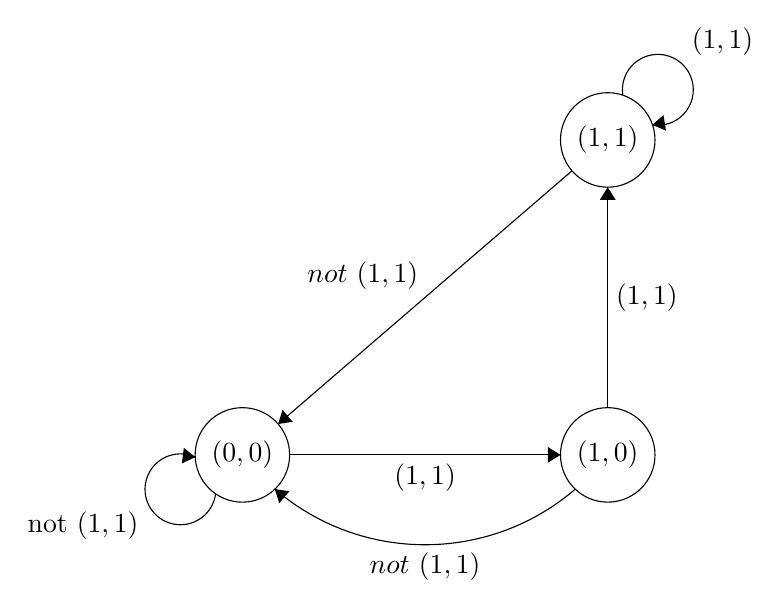
\begin{tikzpicture}[scale=0.2]
	\tikzstyle{every node}+=[inner sep=0pt]
	\draw [black] (28.4,-36.5) circle (3);
	\draw (28.4,-36.5) node {$(0,0)$};
	\draw [black] (51.6,-36.5) circle (3);
	\draw (51.6,-36.5) node {$(1,0)$};
	\draw [black] (51.6,-16.5) circle (3);
	\draw (51.6,-16.5) node {$(1,1)$};
	\draw [black] (31.4,-36.5) -- (48.6,-36.5);
	\fill [black] (48.6,-36.5) -- (47.8,-36) -- (47.8,-37);
	\draw (40,-37) node [below] {$(1,1)$};
	\draw [black] (51.6,-33.5) -- (51.6,-19.5);
	\fill [black] (51.6,-19.5) -- (51.1,-20.3) -- (52.1,-20.3);
	\draw (52.1,-26.5) node [right] {$(1,1)$};
	\draw [black] (26.699,-38.957) arc (-6.96472:-294.96472:2.25);
	\draw (21.83,-40.98) node [left] {not $(1,1)$};
	\fill [black] (25.42,-36.64) -- (24.68,-36.05) -- (24.56,-37.04);
	\draw [black] (49.539,-38.673) arc (-49.35642:-130.64358:14.645);
	\fill [black] (30.46,-38.67) -- (30.74,-39.57) -- (31.39,-38.81);
	\draw (40,-42.71) node [below] {$not\mbox{ }(1,1)$};
	\draw [black] (52.56,-13.67) arc (189:-99:2.25);
	\draw (56.9,-10.25) node [right] {$(1,1)$};
	\fill [black] (54.43,-15.54) -- (55.3,-15.91) -- (55.14,-14.92);
	\draw [black] (49.33,-18.46) -- (30.67,-34.54);
	\fill [black] (30.67,-34.54) -- (31.6,-34.4) -- (30.95,-33.64);
	\draw (36.05,-26.01) node [above] {$not\mbox{ }(1,1)$};
	\end{tikzpicture}
\end{center}
\vspace{5mm}

% Generalize this diagram to labelled transition system
% Transition system is a directed graph

% Transition system, semiautomaton, operator monoid
% F-coalgebra => transition systems are classes (math object)
% Difference between semiautomata and automata

Note that the actual complexity of the concrete cuckoo clock would be a bit more complicated than the automaton above. For example, what does the bird do specifically when it is on? Perhaps it raises and lowers its wings three times, turns its head to the right twice, and repeats. This process can be modeled by a different automaton. To fully model a concrete automaton, we must reduce it to an abstract machine, a system of states and transitions that account for every intended behavior. Abstract machines are capable of modeling systems of any arbitrary complexity. The automaton above is a model of computation called a \textit{finite-state machine} (FSM), and it will be the first abstract machine that we will discuss.
\\

% The nodes could themselves be automata => automata are recursive structures

%----------------------------------------

\subsection{Formalization of an Abstract Machine}

\begin{tcolorbox}[breakable, enhanced, colback=textbook-blue, sharp corners]
	\vspace{3mm}
	\begin{center}
		\textbf{A Brief Introduction to Formal Grammars}
	\end{center}
	A formal grammar is a finite set of \textit{production rules} that specifies what a particular language is supposed to look like. It formalizes the structure of "grammatical units" in a language. This is done in order to enforce a specific alphabet, a consistent lexicon, and a predictable sentence structure, all of which contribute to how useful and distinct any given language is. \\
	
	A grammar $G$ consists of the following components:
	\begin{itemize}
		\item A finite set $N$ of \textit{nonterminal} symbols.
		\item A finite set $\Sigma$ of \textit{terminal} symbols that is disjoint from $N$.
		\item A symbol $S\in N$, designated as the \textit{start symbol}.
		\item A finite set $P$ of \textit{production rules} where each rule is of the form ${(\Sigma\cup N)^*N(\Sigma\cup N)^*\rightarrow(\Sigma\cup N)^*}$.
	\end{itemize}
	
	Put another way, a production rule converts a sequence of symbols to another sequence of symbols. If a rule is of the form \textit{left-hand side $\rightarrow$ right-hand side}, each side can contain terminals and nonterminals, but its left-hand side must contain at least one nonterminal. A nonterminal is a symbol that is replaced by other symbols when an appropriate rule is applied. Unlike a terminal, it does not belong to the alphabet of the language, but rather represents a sequence of symbols that do. Terminals cannot be replaced by other symbols once chosen. \\
	
	Let's construct a simple formal grammar. It is typical for the nonterminals to be uppercase and for the terminals to be lowercase. Let $N=$ \{SENTENCE, NOUN, ADJ\}, $\Sigma=$ \{the, dog, building, plays, fluffy, good\}, and $S=$ SENTENCE. The rules of $P$ are given below.
	
	\begin{itemize}
		\item SENTENCE $\rightarrow$ the NOUN plays
		\item NOUN $\rightarrow$ ADJ NOUN
		\item NOUN $\rightarrow$ dog
		\item NOUN $\rightarrow$ building
		\item ADJ $\rightarrow$ fluffy
		\item ADJ $\rightarrow$ good
	\end{itemize}
	
	We can now start with SENTENCE and apply these rules to construct a "sentence" that is valid in this language. Example sentences and their derivations are given below.
	
	\begin{itemize}
		\item SENTENCE $\rightarrow$ the NOUN plays $\rightarrow$ the ADJ NOUN plays $\rightarrow$ the good NOUN plays $\rightarrow$ the good dog plays
		\item SENTENCE $\rightarrow$ the NOUN plays $\rightarrow$ the ADJ NOUN plays $\rightarrow$ the ADJ ADJ NOUN plays $\rightarrow$ the ADJ ADJ ADJ NOUN plays $\rightarrow$ the fluffy ADJ ADJ NOUN plays $\rightarrow$ the fluffy good ADJ NOUN plays $\rightarrow$ the fluffy good fluffy NOUN plays $\rightarrow$ the fluffy good fluffy building plays
	\end{itemize}
	
	Notice that the first example expresses an actual thought whereas the second example, while still syntactically a sentence, is nonsensical. Because it allows meaningless sentences, the grammar described above belongs to the class of \textit{context-free grammars}.
	
	\vspace{3mm}
\end{tcolorbox}
\vspace{2\baselineskip}

%----------------------------------------

\subsection{Classes of Automata and the Languages They Can Understand}

Automata, in general, are machines that receive, interpret, and follow instructions that are written according to the \textit{grammar} of a \textit{formal language}. Formal languages are similar to the \textit{natural languages} that humans speak in that they have \textit{words} that conform to a \textit{syntax} that is specified in terms of symbols from an \textit{alphabet}. These words can be arranged according to a \textit{grammar} to form \textit{sentences}, from which \textit{semantic meaning} can be interpreted. However, unlike natural languages, they are defined in precise, unambiguous terms. \\

A formal language $L$ over an \textit{alphabet} $\Sigma$ is a \textit{set of words} that is a subset of $\Sigma^*$, the set of \textit{all} possible words that can be composed using $\Sigma$. Typically, formal languages conform to a \textit{formal grammar}, which is a set of precise grammatical rules. However, not all formal grammars are equal. Grammars determine how words can be arranged into sentences, which determines the kinds of thoughts that can be expressed. Thus, grammar controls how \textit{powerful} or \textit{expressive} a language is. If we intend to use a particular formal language to instruct a computer to solve a problem, the \textit{expressiveness} of the language will determine the kinds of instructions we are able to give. If we cannot express a given instruction, we will not be able to solve any problems requiring that instruction. \\

In this section, we will examine automata with different \textit{mechanical structures}. The \textit{data} that are stored in components of these structures can be interpreted as words, and the structures themselves can be used to represent the rules of a formal grammar. However, some expressive grammars cannot be represented by simpler structures. Thus, the mechanical structure of an automaton acts as an \textit{upper bound} on its \textit{capacity} to understand language, and, by extension, its computational versatility. \\

We will now discuss four classes of automata, in increasing order of complexity. As they become more complex, automata are able to recognize more powerful and expressive languages. They can be told to execute \textit{instructions} in these languages, and they will be able to accomplish more complex tasks if their language is more expressive. When we reach the last of these four automata, we will be talking about the most powerful model of computation that is feasible to build, the automaton that models modern general-purpose computers. Once we explore this particularly important automaton in depth, we will learn how it can be modified to model more exotic forms of computation. \\

\subsubsection{Finite-state Machines}

A finite-state machine is a model of computation that can be in exactly one \textit{state} from a finite set of states at any given time. Given its current state and an input, an FSM can \textit{transition} to another state. \textit{Deterministic finite automata} (DFA) are FSMs that transition to at most one state for each input. In contrast, \textit{nondeterministic finite automata} (NFA) can transition to zero or more states for each input. It follows then that a DFA is a special kind of NFA. An FSM may also have a subset of states that are considered \textit{final states}. When the machine transitions to one of these states, it will finish its work and cease operation. \\

FSMs can read and understand \textit{regular languages}, which are languages that can be expressed using a \textit{regular expression} or \textit{regex}. A regex consists of constants (which denote sets of strings) and operators (which denote operations on those sets). If an FSM receives an input (such as a regex) at a given state, and its state-transition function maps that state and input to another state, we say that the FSM \textit{matches} that input. That is, it considers that input valid and will perform an action accordingly. \\\\

\begin{tcolorbox}[breakable, enhanced, colback=textbook-blue, sharp corners]
	\vspace{3mm}
	\begin{center}
		\textbf{A Quick Summary of Regular Expressions}
	\end{center}

	Given a finite, non-empty input alphabet $\Sigma$, there are three constants defined as regexes:
	
	\begin{itemize}
		\item The \textit{empty set}, $\emptyset$, which denotes the set containing no elements.
		\item The \textit{empty string}, $\varepsilon$, which denotes the set containing only the empty string "."
		\item A \textit{literal character} (e.g. the character $a$ denotes the set containing only the character "$a$").
	\end{itemize}
	
	These constants can be combined and manipulated with operators to create long, complex regular expressions. There are three operators that operate on regexes, which are described below in increasing order of priority. Given regular expressions $A$ and $B$, the operations include:
	
	\begin{itemize}
		\item The \textit{concatenation} of $A$ and $B$, $AB$, which denotes the set of strings that can be created by concatenating a string in $A$ with a string in $B$.
		\item The \textit{alternation} of $A$ and $B$, $A|B$, which denotes the union set of $A$ and $B$.
		\item The \textit{Kleene star} of $A$, $A^*$, which denotes the set of all strings that can be created by concatenating a finite number of strings (including zero strings) from the set $A$.
	\end{itemize}
	
	Two additional operators are added as "syntactic sugar": $+$ and $?$. Whereas the literal character $a$ denotes the set of strings that contain a single $a$ and nothing else, the regex $a+$ denotes the set of strings that contain \textit{at least one} $a$ and nothing else and the regex $a?$ denotes the set of strings that contain \textit{at most one} $a$ and nothing else. Thus, $a+=aa^*$ and $a?=a|\varepsilon$. \\
	
	A variety of \textit{metacharacters} are also often used in order to create more concise regexes. Common metacharacters include:
	
	\begin{itemize}
		\item $\hat{}\;$, which matches the starting position in a line of text.
		\item $\$$, which matches the ending position in a line of text.
		\item $.$, the \textit{wildcard}, which matches any character.
		\item $-$, which, when placed between two regexes in brackets, denotes a range of characters.
		\item $[\;\hat{}\quad]$, which matches a single character which is not in the brackets.
	\end{itemize}
	\vspace{3mm}
\end{tcolorbox}
\vspace{2\baselineskip}

Not only is it correct to say that a finite-state machine can understand any regular expression, but also it is true that FSMs and regexes are equivalent. That is, a regex can be written in the form of an FSM and vice versa. Indeed, a regular language "program" can be expressed as a regex, a DFA, or an NFA. For example, the regex [A-Z][a-z]$^*$[0-9] describes any string that starts with a single uppercase letter, is followed by zero or more lowercase letters, and ends with a single digit. This expression can also be represented by the following DFA. Note that state $3$ is circled twice to indicate that it is a final state. The automaton will continue to run until it receives a sequence of input that allows it to transition to its final state.\\

\vspace{3mm}
\begin{center}
	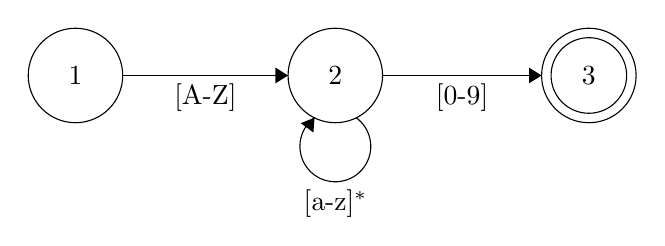
\begin{tikzpicture}[scale=0.2]
	\tikzstyle{every node}+=[inner sep=0pt]
	\draw [black] (22.9,-27) circle (3);
	\draw (22.9,-27) node {$1$};
	\draw [black] (39.4,-27) circle (3);
	\draw (39.4,-27) node {$2$};
	\draw [black] (55.5,-27) circle (3);
	\draw (55.5,-27) node {$3$};
	\draw [black] (55.5,-27) circle (2.4);
	\draw [black] (25.9,-27) -- (36.4,-27);
	\fill [black] (36.4,-27) -- (35.6,-26.5) -- (35.6,-27.5);
	\draw (31.15,-27.5) node [below] {[A-Z]};
	\draw [black] (42.4,-27) -- (52.5,-27);
	\fill [black] (52.5,-27) -- (51.7,-26.5) -- (51.7,-27.5);
	\draw (47.45,-27.5) node [below] {[0-9]};
	\draw [black] (40.723,-29.68) arc (54:-234:2.25);
	\draw (39.4,-34.25) node [below] {[a-z]$^*$};
	\fill [black] (38.08,-29.68) -- (37.2,-30.03) -- (38.01,-30.62);
	\end{tikzpicture}
\end{center}
\vspace{5mm}

Regular languages and, by extension, finite-state machines are often used in string searching algorithms. FSMs and regular languages are also often used in the lexical analysis (lexing) done by a compiler. That is, they give language designers the power to specify which words are valid in their programming language. \\

\subsubsection{Pushdown Automata}

Pushdown automata (PDA) are finite-state machines that also have access to a stack. These automata introduce a notion of \textit{history} or \textit{memory}. A PDA can push a symbol onto its stack on every transition, which will provide information in the future about actions in the past. It can also pop or peek at the stack to decide which transition to take next. \\

Pushdown automata can distinguish syntactically correct sentences from random sequences of valid words, something finite-state automata cannot do because they have no notion of what comes earlier than a given point in a given sentence. For example, a pushdown automaton would be able to tell that "my dog bites red toys" is a valid English sentence and "red my toys dog bites" is not. However, PDA cannot understand semantics. It would also consider "my dog \textit{barks} red toys" a valid English sentence, even though it has no meaning. \\

Pushdown automata can read \textit{context-free languages}, which are languages that follow a \textit{context-free grammar}. Context-free languages are formal languages whose production rules are of the form $A\rightarrow\alpha$ where $A$ is a nonterminal and $\alpha$ is a sequence that may contain terminals and nonterminals. A PDA pops terminals from its stack. When a nonterminal $A$ is at the top of the stack, the PDA can pop it and push the $\alpha$ of some production rule onto the stack. In a sense, the stack of the PDA contains the unprocessed data of the grammar. \\

Context-free grammars can be written to formalize languages such as the language of matching parentheses or the language of infix algebraic expressions (e.g. (2+4)/7*8). PDA and context-free languages are often used in the syntactic analysis (parsing) done by a compiler. That is, they give language designers the power to specify how valid sentences are structured in their programming language. \\

\subsubsection{Linear Bounded Automata}

Imagine that, instead of a stack, an automaton could have access to a finite-length list. Linear bounded automata (LBA) have a finite number of \textit{states}, a finite length of \textit{tape}, and a \textit{head} that can read and write symbols on the tape and move left or right along it, one symbol at a time. The length of the tape is a linear function of the length of the input, so we can say that the tape has $kn$ cells, where $n$ is the length of the input instructions and $k$ is a constant. \\

This machine is similar to the idea of a modern computer. The tape represents a finite amount of memory, and the head is able to read and write to it. LBA can understand \textit{context-sensitive languages}, which are languages that follow a \textit{context-sensitive grammar}. Sophisticated programming languages are context-sensitive, so a linear bounded automaton would be able to read and understand modern software. The $kn$-length tape acts as a sufficient environment for computationally demanding programming tasks, given a large enough $k$. Similarly, given enough memory, real computers can also solve very computationally difficult problems. \\

A context-sensitive language is a language where semantics matter. Using our earlier example, "my dog barks red toys" would not be a valid sentence in a context-sensitive version of English. An LBA then is actually able to differentiate data types and can tell when an operation is defined for one type and undefined for another. LBA and context-sensitive languages are often used in the semantic analysis (type checking) done by a compiler. That is, they give language designers the power to specify whether or not a syntactically correct sentence actually has any real \textit{meaning} in their programming language. \\

Where can we go from here? LBA are suitable models of real-world computers, and they can process semantic language. What more can we do? Let's try making the tape infinitely long$\dots$ \\

\subsubsection{Turing Machines}

A \textit{Turing machine} (TM) not only models real-world computers, but \textit{computation} itself. The concept, which was formalized in 1936 by Alan Turing, generalizes automata and defines the limitations of mechanical computing. It specifies a set of components that are necessary and sufficient for creating a "problem-solving machine" that is capable of solving any problem that can be solved by a machine. Weaker automata can solve \textit{some} of these machine-solvable problems, but only \textit{Turing-complete} automata (those that are functionally equivalent to TMs) have the expressive power to solve \textit{any} of them. The components of a Turing machine are listed below.

\begin{itemize}
\item An infinitely long \textit{tape} that is divided into cells, each of which contains a symbol from some finite alphabet. One symbol from this alphabet is considered blank, and the tape is initially filled with these symbols.
\item A \textit{head} that can read and write symbols on the tape and move left or right along it, one symbol at a time.
\item A \textit{state register} that stores its current state and initially stores its starting state.
\item A \textit{finite table of instructions} that, given the machine's current state and tape symbol, tells the machine to do the following sequence of actions:
	\begin{enumerate}
		\item Erase or write a symbol at the current tape cell (or do nothing)
		\item Move the head one tape cell to the left or right (or do nothing).
		\item Depending on the current state and input, transition to a different state (or the same state) or halt computation.
	\end{enumerate}
\end{itemize}

A machine like this need not be a real-world computer. In fact, in his original proof, \textit{On Computable Numbers, with an Application to the Entscheidungsproblem}, Turing refers to a person, whom he calls the "computer," as an example of a Turing machine. If we break down these components into the resources they represent, it becomes clear that many systems could be considered Turing machines.

\begin{itemize}
	\item The infinitely long tape represents \textit{infinite space for computation} or \textit{infinite memory}.
	\item The head represents three abilities:
		\begin{enumerate}
			\item Reading memory,
			\item Writing to memory,
			\item Traversing the memory freely, with no side effects.
		\end{enumerate}
	\item The state register represents the ability to \textit{know what "step" you are on} in the problem-solving process. We will clarify this ambiguous idea in a second, but for now just think of it as having an idea of your progress.
	\item The finite table of instructions represents a \textit{sequence of commands} or \textit{program} that can be followed unambiguously. The automaton can follow and obey these commands in order without any actual thought.
\end{itemize}

As long as you have unlimited space to work in, the freedom to read and write symbols anywhere in that space, a list of instructions to follow exactly, and the knowledge of what to do next, you have a Turing machine. We can now visualize the person Turing referred to as a "computer." It is a man with an infinitely large piece of paper, a pen that he writes symbols with, a list of instructions that tells him which symbols to write, where on the paper to move his pen tip, which instruction to perform next, and a knowledge of which instruction he is currently performing. Many systems of logic, such as programming languages, are Turing-complete. Many things not traditionally thought of as "systems of logic" are \hrefcolor[blue]{https://www.toothycat.net/~hologram/Turing/index.html}{\underline{also Turing-complete}}. \\\\

\begin{tcolorbox}[breakable, enhanced, colback=textbook-blue, sharp corners]
	\vspace{3mm}
	\begin{center}
		\textbf{Turing Machines and Consciousness}
	\end{center}
	In 1950, Turing developed the \textit{Turing test}, a test of a machine's ability to exhibit behavior indistinguishable from that of a human. It involves an interrogator who is tasked with having two separate text conversations and determining which of the two participants is actually a machine. If the interrogator cannot distinguish a difference, the machine has passed the test. Despite its importance to the philosophy of computer science, the test is not a good indicator of whether or not a computer can think. The test says more about how gullible the interrogator is than how conscious the computer is. At the end of the day, the computer is still following its programming. \\
	
	What about this man whom Turing calls a "computer"? Would he pass the test, given the right programming? Perhaps he would. But that would not make him a \textit{person}. What kind of person is this man if he follows whatever instructions he is given? He is a slave, a person who always obeys. Could we say then that machines are also, in a certain sense of the word, slaves? Perhaps this is where the term \textit{master-slave technology} came from. Regardless, it is important to make a philosophical distinction here about what separates humans from machines or, more precisely, what distinguishes \textit{thought} from \textit{computation}. \\
	
	Essentially, this boils down to the question of consciousness. There is much debate about consciousness. Philosophers have proposed a variety of concepts that partially define it such as free will (the ability to choose) or qualia (the raw experience of existence, e.g. sounds, colors, emotions). However, \textit{intentionality} is one characteristic that is generally agreed upon as necessary for conscious thought. Intentionality is the ability of the mind to think \textit{about} something. Computers can \textit{think} things, but they cannot \textit{think about} things. They lack intentionality.\\
	
	For a Turing machine, the list of instructions is an essential component. It is capable of "thinking" if and only if some one tells it what to think. That effort is more accurately defined by the term "computation." We would also refer to the man's efforts with his pen and infinite paper as computations because they require no thought. If he were nothing more than a Turing machine, the man would not be able to perform mathematics on his own. In fact, he would not be able to do anything without instructions. It is the moment when he does something without being explicitly told to do it that he first displays consciousness. When \textit{unprompted} computation is performed for some \textit{purpose}, we can talk about consciousness. \\
	
	So calling computers slaves is a bit of an anthropomorphization. A slave is a conscious being who is forced to act like a machine. Computers don't have the prerequisite consciousness. No matter how complicated its architecture or sophisticated its artificial intelligence software, a computer is a \textit{tool} like a microwave or a calculator. Could it ever be more than that? Could a technology ever think? \hrefcolor[blue]{https://en.wikipedia.org/wiki/Artificial\_consciousness}{\underline{Perhaps}}. But such a thing would be quite different from a Turing machine or any modern computer. \\
	
	\parbreak
	\vspace{1mm}
	
	\begin{displayquote}
		\textit{In attempting to construct such machines we should not be irreverently usurping His power of creating souls, any more than we are in the procreation of children: rather we are, in either case, instruments of His will providing mansions for the souls that He creates.}
		\vspace{4mm}
		\begin{flushright}
			---Alan Turing (1950), \\
			in response to a theological objection to artificial consciousness.
		\end{flushright}
	\end{displayquote}
	\vspace{3mm}
\end{tcolorbox}
\vspace{2\baselineskip}

A single-tape Turing machine is formally defined as a septuple $(Q,\Gamma,b,\Sigma,\delta,q_0,F)$, where

\begin{itemize}
	\item $Q$ is a finite, non-empty set of \textit{states},
	\item $\Gamma$ is a finite, non-empty \textit{tape alphabet},
	\item $b\in\Gamma$ is the \textit{blank symbol},
	\item $\Sigma\subseteq\Gamma\setminus \{b\}$ is the set of symbols that can be written on the tape,
	\item $\delta$ is a partial function $\delta : (Q\setminus F)\times\Gamma\nrightarrow \Gamma\times\{L,R\}\times Q$ called the \textit{transition function}, which inputs the current state and tape symbol and outputs the symbol to write to the tape, the direction to move the head, and the next state to transition to,
	\item $q_0\in Q$ is the \textit{starting state}, and
	\item $F\subseteq Q$ is the set of \textit{final states}. The contents of the tape are \textit{accepted} if the Turing machine halts computation in a state from $F$.
\end{itemize}

We should now address what exactly "state" is in regard to computing. Many people associate it with the current instruction being fed to the machine. However, Turing made a distinction between this interpretation of state and the interpretation of state as the computer's "progress" or "state of mind." Turing's \textit{complete configuration} of state includes not only the current instruction, but the current symbol configuration of the entire tape as well and all the instructions yet to be executed. In this way, state is defined by the results of past instructions and the inevitable execution of future instructions. \\

Now we have defined what a Turing machine is, but it is still not clear why it is considered such a landmark concept in computer science. For example, if real-world computers can be sufficiently modeled by linear bounded automata, why do we instead focus so heavily on Turing machines? \\

Turing machines are the class of automata that can read \textit{recursively enumerable languages}. A formal language is called recursively enumerable, if it is a \textit{recursively enumerable subset} in the set of all possible words over the alphabet of the language. This essentially means that, for a language of this type, there exists an algorithm that can output a list of every word in the language. Consider what would be required for such an algorithm. How many valid words are there in a given language? Depending on its rules for constructing words, there may be an infinite amount. This is the case for some programming languages. A variable name could theoretically be as long as you want, provided you have enough memory to store it. In order to list all of the words in a recursively enumerable language, you would need infinite memory, which only a Turing machine can provide. \\

This does not imply that TMs can handle infinite lists of instructions. Rather, they can handle \textit{infinite looping} over a finite set of instructions. A Turing machine can "successfully" run a never-ending program. A real machine would use up all of its memory trying to run such a program, eventually crashing due to a \textit{stack overflow} (an attempt to write data outside of the limits of the memory). A TM would never run out of memory and, given infinite time, could run the program forever. \\

As previously stated, the Turing machine models not only computers, but \textit{computation}. It abstracts away the physical limitations of computers such as memory constraints, overheating, or hardware failure and asks what the fundamental limits of algorithmic computation are. It makes a statement on which mathematical problems are \textit{decidable}. It is an ideal computer, and, as such, it is not only a model of what real-world computers are today, but a model of what they \textit{could be} in the future, given sufficient advances in hardware. \\

%----------------------------------------

\subsection{The Importance of Turing Machines to Modern Computing}

The automata we have discussed so far (finite-state machines, pushdown automata, linear bounded automata, and Turing machines) form a sort of hierarchy of machine capability. The formal grammars and languages that these automata can understand likewise constitute a hierarchy that was first described by Noam Chomsky in 1956. The \textit{Chomsky hierarchy}, a classification of the expressiveness of language according to grammatical rules, is summarized below by a table with columns for grammars, the languages those grammars build, and the class of automaton that can understand those languages.

\begin{table}[H]
	\caption{The Chomsky Hierarchy}
	\label{tab:LABEL}
	\begin{tabularx}{\textwidth}{|c|c|Y|}
		\vtabularspace{3}
		\hline
		Grammar & Language & Automaton \\
		\hline
		Type-0 & Recursively enumerable & Turing machine \\
		Type-1 & Context-sensitive & Linear bounded automaton \\
		Type-2 & Context-free & Pushdown automaton \\
		Type-3 & Regular & Finite-state machine \\
		\hline
		\vtabularspace{3}
	\end{tabularx}
\end{table}

As this is a hierarchy, higher-ranking automata are capable of doing anything that lower-ranking automata can. For example, an LBA can do anything that a PDA or FSM can and \textit{more}. To give a linguistic analogy, an LBA would be fluent in all of the languages that the PDA and FSM are fluent in, but would also be fluent in additional languages. What causes this difference in language facility? It is the structure of the automaton's memory. \\

Let's recap how these four automata handle memory.

\begin{itemize}
	\item An FSM has \textit{no} memory. It simply has a finite number of states, perhaps represented by a finite list of instructions. It can transition between states, but it has no notion of how it got to any particular state. It records no history.
	\item A PDA has a \textit{stack} of memory, but this form of memory is restricted. It cannot read or write its memory in any order it likes. It can read the top entry on the stack, but it must delete data to read entries located elsewhere.
	\item An LBA has a \textit{finite array} of memory. It can read or write this memory in any order it likes, but it has limitations on how much information it can store.
	\item A TM has an \textit{infinite array} of memory. It can read or write this memory in any order it likes, and it can also store as much as it likes.
\end{itemize}

It is no coincidence that real-world computers today use array-based memory. Arrays are both an intuitive and Turing-complete way to store information. Now, technically, LBA and TMs use "tape" instead of arrays, but the differences are minimal. In tape memory, cells have relative position, but they are not \textit{labeled}. Modern computers are actually modeled by \textit{register machines}. Register machines are equivalent in expressive power to Turing machines, but their memory is composed of an infinite-length array of uniquely addressed \textit{registers}. Like a tape of cells, an array of registers can be freely accessed. \\

A subset of register machines known as \textit{random-access machines} allow for \textsc{jump} instructions (e.g. jump to register \#5623) in addition to standard sequential traversal of memory (e.g. move right, move right, move right, etc). This allows computers to accomplish a task with fewer instructions, but the expressive powers of random-access machines and Turing machines are equivalent because both are capable of \textit{eventually} solving the task. Modern computers can be described as random-access machines because they use \textit{random-access memory} (RAM). In RAM, the time to access information is independent of physical location. From a performance perspective, this means that we do not have to consider \textit{where} we store things in memory. It's all uniformly fast. This allows for the construction of \textit{node-based} data structures, which we will discuss in a later section. \\\\

\begin{tcolorbox}[breakable, enhanced, colback=textbook-blue, sharp corners]
	
	\vspace{3mm}
	
	\begin{center}
		\textbf{Exploring Exotic Automata}
	\end{center}

	It is worth thinking about automata whose memory is modeled by non-list data structures. For example, a pushdown automaton uses a stack to model its memory and because of this, it is not Turing-complete. What if it used a queue instead? In this case, it would be Turing-complete because it could dequeue items to traverse the memory and then enqueue them to avoid data loss. One could envision this as a Turing machine whose infinite tape ends are glued together to form an infinite loop. The machine can only move in one direction, but it can still access every cell because its tape is circular. \\
	
	The memory can also be modeled by non-sequential data structures to create some bizarre models of computation. What if the memory of a computer was laid out not as an array, but as an undirected tree? What if it was organized according to an algebraic structure like a monoid or a ring? I'm not even going to pretend that I understand what kind of behavior this would result in. But it is an \hrefcolor[blue]{https://kluedo.ub.uni-kl.de/frontdoor/index/index/docId/4400}{\underline{area of active research}}. \\
	
	Other tweaks can be made to the properties of a Turing machine to create new, interesting automata. For example, \textit{$\omega$-automata} (or \textit{stream automata}) are Turing machines that expect an \textit{infinite} sequence of instructions. \textit{$\omega$-automata} never stop running because an infinite sequence of instructions requires an infinite sequence of instruction executions. Because they never terminate, they never move into acceptance (final) states. Rather than a set of final states $F$, they have a set of \textit{acceptance conditions} $Acc$. \\
	
	For ordinary automata, every \textit{run} $\rho$ (i.e. a sequence of $n$ states) ends with a state $r_n$, and the input is only accepted if this state is final (i.e. $r_n\in F$). For $\omega$-automata, runs are infinite sequences, so they do not end with a state $r_n$ at all. How do we tell if a run $\rho$ should be accepted as a valid set of instructions? We require that $\rho\in Acc$. That is, if the run is a member of the "set of acceptable runs," it should be accepted. What is the "set of acceptable runs"? That depends on which variant of $\omega$-automaton you are talking about. \\
	
	The class of $\omega$-automata contains multiple automata with different definitions of $Acc$. For example, for some subset $F$ (final states) of $Q$ (all states), the \textit{B\"{u}chi automaton} accepts those runs $\rho$, for which there exists a final state that occurs "infinitely often" in $\rho$. What is a state that is visited "infinitely often"? Given an infinite amount of runtime, some states in $Q$ will be visited an infinite amount of times, and others will not. For example, what if you can transition away from your starting state $q_0$, but you are not allowed to transition into it. Even given infinite time, $q_0$ would not be visited infinitely often, and if it were the only state in $F$, you would never be able to construct a run that would be considered valid by a B\"{u}chi automaton. Nondeterministic B\"{u}chi automata have applications in "always-on" or "always listening" software, such as those used in highly-autonomous robots or smart speakers like the Amazon Echo, both of which receive instructions based on a never-ending, real-time stream of sensory data. \\
	
	Wow, that's a lot of abstract mathematics. Why is any of this important for gaining a fundamental understanding of Turing machines or real-world computers? It is important because we can only really grasp their \textit{scope} if we explore outside of it. Some automata can have properties that are not practical or possible to implement in the real-world. Mathematically, they could have infinite states or continuous alphabets or hyperdimensional memory. But here, once and for all, let's define the scope of computation we will be considering for the rest of this guide. \\
	
	A modern computer has:
	
	\begin{itemize}
		\item A \textbf{finite} set of states Q. If it were instead infinite, the automaton would have a state for every possible input, and thus would be able to understand any conceivable language. This is far too powerful a machine to build. This would essentially be a universal problem solver.
		\item A \textbf{finite} alphabet $\Sigma$. If it were instead infinite, the automaton could have a continuous alphabet. What kind of alphabet's symbols exist on a spectrum? Perhaps you could call \textit{sound} a "language" with a continuous alphabet known as frequency. An automaton with an infinite alphabet would not be digital and would not use bits. It would be an analog computer. Analog computers do exist, and they were popular in the 1950s and 1960s, but nowadays we write software for digital computers. \textit{Fun fact:} analog synthesizers, which are still commonly used in electronic music, are considered a kind of analog computer.
		\item A transition \textbf{function} $\delta$. If it were instead a relation (i.e. inputs are mapped to more than one output), the automaton would be nondeterministic. It is suspected that nondeterministic Turing machines would be able to solve NP-complete problems, which is a computational feat that has not yet been accomplished in a tractable way by a deterministic Turing machine.
	\end{itemize}

	\vspace{3mm}
	
\end{tcolorbox}
\vspace{2\baselineskip}

While more exotic memory structures are theoretically possible, real-world computers use \textit{arrays} of memory. Since Turing machines can solve any computable problem and data structures are used by computers to solve problems, it follows that data structures can be simulated by Turing machines. Because register machines use array-based memory and are Turing-equivalent, it also follows that \textbf{all data structures can be implemented using arrays}. This is a very useful insight, and it will be discussed further in Section 3. \\

The selection of Turing machines (or register machines) as the model for real-world computers has also influenced decisions in computer architecture. In early computers, the instructions were not integrated into the machine. Code was written on punch cards, which were fed into computers. Eventually, code was stored digitally in programs that were uploaded to the computer's memory. This type of machine is known as a \textit{stored-program computer}. \\

Where should one store instructions or code in a stored-program computer? Those that have a \textit{Harvard architecture} store their instructions in an \textit{instruction memory} that is separate from the \textit{data memory}. Those that have a \textit{von Neumann architecture} store their instructions and data in the same physical memory, but partition the memory somehow to avoid overwriting the instructions. The von Neumann architecture allows "programs that write programs," such as assemblers, compilers, linkers, and loaders. Modern computers are more von Neumann than they are Harvard because their instructions and data share an address space, but they are not strictly either. We can describe modern computers as \textit{random-access stored-program} (RASP) machines with \textit{split-cache modified Harvard architectures}. \\

%----------------------------------------

\subsection{Modern Hardware Implementation}

% We've discussed "computers" in many different ways (primitive examples, pre-Turing examples, theoretically).
% The typical modern computer is programmable (in a Turing-complete sense), digital, electronic, stored-program, general-purpose, uses RAM, uses so-and-so architecture
% Maybe some ubiquituous devices and "optional" components (like hard drives and I/O)
% Maybe discuss some important non-standard computers (embedded systems, datacenters, supercomputers).

% Signals, clock cycles
% Byte vs word addressing
	
%--------------------------------------------------------------------------------
%    SECTION: COMPUTABILITY THEORY
%--------------------------------------------------------------------------------

\toclineskip
\section{Computability Theory}

\vspace{4mm}
\begin{displayquote}
\textit{Thirty years ago, we used to ask: Can a computer simulate all processes of logic? The answer was yes, but the question was surely wrong. We should have asked: Can logic simulate all sequences of cause and effect? And the answer would have been no.}
\begin{flushright}
	---Gregory Bateson
\end{flushright}
\end{displayquote}
\vspace{4mm}

% Algorithm characterizations (wiki)

Computation is mathematical in nature. Underneath its shiny UI and immersive applications, a computer is simply a machine that can be programmed to calculate numbers (and do it \textit{very} quickly in the case of modern computers). With that said, let me pose the central question of computability theory: could a machine (or computer) theoretically solve any given math problem, if given the correct input (or code)? We will consider this question more formally in this section, but it turns out that the answer is no. There exist problems that a computer will never be able to solve with computation, even given infinite resources. \\

In this section, we will discuss what makes a problem \textit{solvable} and thus within the scope of computational analysis. We will also briefly discuss \textit{unsolvable} problems and how they can be organized into a hierarchy of \textit{unsolvability}. That said, before we discuss either solvable or unsolvable problems, we need to formalize our definition of the term \textit{problem} with regard to the field of computer science. \\

%----------------------------------------

\subsection{The Scope of Problem Solving}

% Rewrite -- what are problems, why are they worth solving, what is calculation, what is computation?

% Domains of discourse / universes in classical logic are just types in type theory. Top = true in every universe, Bottom = true in no universes (false)

% Use sequent notation to explain axioms
% Formal systems
% Proof calculi (Hilbert)
% Automata are formal systems

Since computation is mathematical, it follows that the natural use of computers is to solve \textit{mathematical problems}. A mathematical problem is a problem that is amenable to being represented with mathematics. Are there problems that are not mathematical? That is, are there problems that either \textit{cannot} be formalized with mathematics or \textit{should not} be formalized with mathematics because the result would produce no valuable insight? Of course. You might say that certain "human" problems are not mathematical in nature. For example, can an ethical problem be solved \textit{mathematically}? Furthermore, what does it mean for a problem to have a mathematical solution? It turns out that the answer lies in the difference between \textit{reasoning} and \textit{logic}. \\

% Curry-Howard: proofs and programs are the same thing. 

% A deductive system is a "calculus"
% Argument - set of statements (premises) and a conclusion in a language
% Premises can be axioms or theorems
% Logical consequence
% Truth-bearer
% Deductive reasoning is applied to an argument to create a deduction (argument + steps of reasoning)
% Composing a deduction is a way to prove validity
% Composing an induction is a way to assess strength
% Venn diagrams
% Reasoning is a set of rules of inference
% Inductive/deductive "steps"
% Proof - deduction from "known truths" (axioms and proven theorems), proves soundness
% Data validation proves cogency?
% Argument vs explanation
% Validity/soundness

\subsubsection{Informal Logic}

% Discuss the logical reasonings comparatively. 3 paths in life. Certain vs uncertain. Binary vs multi-valued.

% Interlocuters
% Fallacious reasoning
% Formal vs informal (indep of interpretation)

\subsubsection{Formal Logic}

% Common logical symbols wiki
% Domain of discourse / universe
% Deduction is impossible in non-axiomatic systems because we don't know what the axioms of the Universe are.

% What is logic?
Logic is a long-standing, far-reaching field, and its definition has changed over the ages, but it can be broadly described as the study of \textit{argument}. 

% What is early logic?
The practice and analysis of logic can be done in many different ways. For example, the early study of logic was mostly done in the context of \textit{natural language} arguments made during oration.

% Syllogistic logic (categorical reasoning, motivated by science 13:45)
% Stoic logic

% Informal logic is not always explicit. It may have implicit elements that must be made explicit by analysis.
% Formal logic, traditionally symbolic logic, now called mathematical logic

% What is modern logic? ("Arguments and the forms they make take")
Modern logic, however, is \textit{formal}. That is, it observes the abstract \textit{forms} of arguments instead of the arguments themselves. \\

% Hobbes - thought as computation
% Boolean logic
% Frege, logicism
% Class - Russell's paradox

Formal logic is the study of \textit{inference} with regard to \textit{formul{\ae}}. Formul{\ae}, Latin for "small forms" or "small rules," are finite sequences of symbols from an alphabet. They are purely \textit{syntactic objects}, much like strings of text. Inference is the act of processing a formula $A$ and deducing that a formula $B$ is a \textit{logical consequence} of $A$. This means that, given a set of \textit{rules of inference}, the string $A$ can be transformed into the string $B$ by means of a finite series of applications of said rules. \\


% Logical and non-logical symbols
% Categorematic and syncategorematic terms (individual meaning)
% Formal systems
% Reason vs. logic -> Humans vs. computers
% Model theory

% Set theory is intertwined with two-valued logic via the membership function

% Fuzzy set theory
% Membership functions between 0 and 1

and they are studied in within \textit{formal systems}. These systems of abstract thoughts are used to infer the existence of formul{\ae} by means of logical deduction starting from a given set of axioms. A formal system has:

\begin{enumerate}
	\item A finite \textit{alphabet} of \textit{symbols}, from which a formula may be constructed
	\item A formal \textit{grammar}, to which a formula must conform if it is to be considered \textit{well-formed} in the system
	\item A set of initial formul{\ae}, known as \textit{axioms}, from which inferences can be made
	\item A set of inference rules, known as a \textit{logical calculus}, which prescribe how inferences are to be made
\end{enumerate}

%%%

Formul{\ae}, which are finite sequences of symbols from a system's alphabet, are purely \textit{syntactic} objects, but, given an \textit{interpretation}, they can be endowed with \textit{semantic} meaning. For example, an interpretation of first-order logic requires the following assignments of semantic meaning:

\begin{enumerate}
	\item Variables are assigned \textit{objects} (things that can be modeled) from a \textit{domain of discourse} (a well-defined set of objects)
	\item Predicates are assigned \textit{properties} of objects
	\item Formul{\ae}, which contain variables and predicates, are assigned a \textit{truth value} of true or false
\end{enumerate}

A well-formed formula with such an interpretation is called a \textit{sentence}, and the meaning expressed by a sentence is called a \textit{statement} or \textit{proposition}. A sentence expressing a true statement (according to the axioms and inference rules of the formal system) is called a \textit{theorem}, and a set of theorems is called a \textit{theory}. For example, ZFC set theory is a first-order \textit{theory} of sets. It has a collection of theorems written in first-order logic that form an \textit{axiomatic set}, and these theorems are used to prove other theorems that also belong to the theory using a set of inference rules. \\

\subsubsection{Decision Problems and Function Problems}

First-order logic is also called \textit{predicate calculus}. It is a system for calculating \textit{predicates}, which are Boolean-valued functions. In mathematics, a predicate maps \textit{propositions} written in first-order logic to Boolean values (i.e. $P:X\rightarrow \{\textsc{true},\textsc{false}\}$). In linguistics, a proposition can be written in the form of a \textit{yes-no question} without sacrificing any semantic meaning. For example, evaluating the proposition "The sky is blue." as true or false is the same thing as answering the question "Is the sky blue?" with either yes or no. \\

More generally, a predicate is a function that receives an input and makes a binary decision about it. In computability theory, the analogous concept is called a \textit{decision problem}, a problem that can be posed as a yes-no question. Decision problems are fundamental to mathematical practice. A proof of a mathematical statement is a decision problem. Additionally, formal verification of a proof involves solving a series of decision problems regarding whether or not each statement in the proof can be reduced to its axioms. The proof is valid if and only if all of its statements are. Decision problems are problems that can be solved by \textit{making a decision} (mapping the question to a yes-no answer).  \\

It is natural to expect that computers, which are tools for doing math, should be able to solve decision problems. That said, computers can handle more than just Boolean-valued functions. They can represent functions of \textit{arbitrary} return type (e.g. integers, words, objects, etc.). This allows them to solve the broader class of \textit{function problems}, problems where a single output is expected for every valid input. Function problems are problems that can be solved by \textit{calculating a function} (mapping the problem input to a solution output). \\

One important example of a decision problem is whether or not a given function problem is solvable. Let $F$ be a \textit{function problem}, and let $D$ be the \textit{decision problem} of whether or not $F$ is solvable for each of its inputs. Let $f:X\rightarrow Y$ be a \textit{function} that solves $F$, where $X$ is the set of all problem inputs and $Y$ is the set of all problem outputs. Let $G(f)$ denote the set of all ordered pairs $(x,f(x))$ such that $x\in X$. $G(f)$ is known as the \textit{graph} of the function $f$. Let $d:X\rightarrow \{\textsc{true},\textsc{false}\}$ be a decision that solves $D$. For each $x\in X$, $d(x)$ is $\textsc{true}$ if and only if there exists an ordered pair $(x,f(x))$ in $G(f)$. Otherwise, $d(x)$ is $\textsc{false}$. \\

Here's a more concrete example. Let $x$ be any natural number (including 0). $F$ asks "What is $\rfrac{2}{x}$ for all $x$?." $D$ asks "Does $\rfrac{2}{x}$ exist for all $x$?." In both cases, $f(x)=\rfrac{2}{x}$, but $F$ is interested in the \textit{value} of each of the outputs while $D$ is interested in the \textit{existence} of each of the outputs. There is one input for which $f$ has no defined output and that is $x=0$. In this case, the answer to $D$ is negative, and $F$ is technically unsolvable. That said, we can just move the goalposts a little bit to make $F$ solvable by allowing $f$ to be a partial function: $f:\mathbb{N}\nrightarrow \mathbb{N}$. Partial functions do not necessarily map every member of their domain to a value. Thus, they can be \textit{undefined} for some input values. As long as "undefined" is considered a valid answer to $F$, $F$ can be considered solvable for its whole domain. \\

In computability theory, we are interested in determining whether or not an output exists for each of a problem's inputs. If an output exists, we can be sure it has \textit{a} value, but the particular value is inconsequential. While computers do solve function problems, it is enough to consider only the corresponding decision problem when proving whether a function problem is \textit{solvable} or not. \\

\subsubsection{"Effective Calculability"}

Before the study of computer science, mathematicians sometimes informally described functions as \textit{effectively calculable}. This meant that a correct output could be calculated for any input from the domain of the function, using an \textit{effective method}. A method, in general, is just a "procedure" that does "something." A method is \textit{effective} if it consists of a finite number of instructions and solves a particular problem. \\

A particular method can be effective for some problems and ineffective for others. For example, typing is a method. If I want to put characters into a text document, typing is an effective method. If I want to plant a flower, typing is not an effective method. However, if I want to plant a flower, building a flower-planting robot and programming it, via typing, to plant a flower \textit{is} an effective method because it actually accomplishes the objective. An effective method that is used to calculate the values of a function is called an \textit{algorithm}. \\

Much work was done in the 1930s to formalize "effective calculability." The results established \textit{Turing computability} as the correct formalization. This model gives the following fundamental definition: any function whose outputs can be calculated by an algorithm is a \textit{computable function}. Computable functions are precisely those functions that can be computed by a Turing machine. In the mathematical sense, they could also be called \textit{solvable}. A computable or solvable \textit{decision} is predictably called \textit{decidable}. If the functions model mathematical proofs, they could also be called \textit{provable}. Despite a few minor differences, all of these terms get at the same idea. \\

We will now discuss the history preceding and the circumstances of this foundational work in formalizing "effective calculability" as computability. Much of this work was done between the 1930s and the 1950s, but it built heavily on set-theoretical concepts discovered by German mathematician Georg Cantor in the late 19th century. After a crash course in Cantorian set theory, we will examine computable functions from a variety of angles. Computability is interdisciplinary. The concept \textit{permeates} our reality, and as such its eventual formalization was made possibly by the collective efforts of mathematicians, logicians, linguists, and computer scientists. Today, research on computability is widespread in the study of anything scientific. \\

After a rigorous study of what is computable, we will conclude this section with a brief exploration of what is not computable. This is a topic that is important to theoretical computer science. By assuming that certain aspects of an abstract machine are \textit{hypercomputational}, we can envision the kind of problems that could be solved if computation were ever to transcend Turing machines. \\

%----------------------------------------

\subsection{The Ballad of Georg Cantor}

Georg Cantor (1845-1918) was a German mathematician whose work established \textit{set theory}, a fundamental theory in mathematics. Much of his work was built on generalizations of the set of natural numbers, namely the \textit{ordinal numbers} and the \textit{cardinal numbers}. These sets include both finite and \textit{infinite} quantities, a concept that was considered very controversial in the late 19th century. Despite an extreme amount of backlash, Cantor stood by his set theory and formalized what has been called "the first truly original idea in mathematics since those of the Greeks." \\

% Introduce the problem of the "size" of infinity.
% Example of the unit circle. The unit circle has a circumference of $2\pi$. It has circumference values of $[0,2\pi]\in\mathbb{R}$. Another way of saying this is that it has \textit{central angle} values of $[0,2\pi]\in\mathbb{R}$. The difference between that and, say, $a_n=\frac{1}{4}*n, n=[0,7]\in\mathbb{Z}$ is that all real intervals have an infinite number of possible values. But what happens when you go past 2\pi, \textit{beyond infinity}. You expand the infinite interval\dots to a another infinite interval. You'd be hard-pressed to find someone who argues that the interval $[0,4\pi]$ is \textit{not} bigger than $[0,2\pi]$. And yet, the intervals have the same "density" (they both have an infinite number of values). So the space doubled, and the density remained the same. This is not familiar to us. "Size" (number of elements) is not a useful measure of infinite sets. We need to generalize to cardinality.
% Are there infinite sets of different cardinalities? What if you doubled your interval an infinite amount of times?

% Trying to work directly with absolute infinity is trouble. Singularities.

\subsubsection{The First Article on Set Theory}

Cantor began his work in number theory, until his mentor, Leopold Kronecker, suggested that he answer an open question in real analysis: "If a given function can be represented by a trigonometric series, is that representation unique?." A trigonometric series is a series of the form
\begin{align*}
\frac{A_0}{2}+\sum_{n=1}^{\infty}(A_n\cos nx + B_n\sin nx).
\end{align*}
One common example of a trigonometric series is a Fourier series, which has coefficients $A_n$ and $B_n$ of the form
\begin{align*}
A_n&=\frac{1}{\pi}\int_{0}^{2\pi}f(x)\cos nx\,dx, \\[1mm]
B_n&=\frac{1}{\pi}\int_{0}^{2\pi}f(x)\sin nx\,dx,
\end{align*}
where $f$ is an integrable function. That said, Cantor's work concerned the general definition of a trigonometric series. He proved that any countable, closed set of natural numbers could encode a trigonometric series that uniquely represents a function. The qualifiers \textit{countable} and \textit{closed} are significant. A countable set is a set whose elements can be counted or enumerated. A closed set is a set that contains its limit points. For a trigonometric series, this means the set of all $n$ must contain a countable number of elements, two of which must be $1$ and $\infty$. $1$ is no problem, but what does it mean for a set to contain $\infty$? And, for example, how can the natural numbers between and including $1$ and $\infty$ be "countable"? \\

The concept of infinity had been around for a long time by the 1870s, but it had, until this point, been considered a philosophical topic. Aristotle identified a dichotomy between the "potential infinite" and the "actual infinite" in which the former can always have elements added to it while the latter is instead considered "complete." This mindset persisted for around two-thousand years with the majority of scholars believing that "actual infinity" was outside of the purview of mathematics. It was used in mathematical practice, but only in a non-rigorous, conceptual way, as seen in the characterization of limits "tending toward infinity." Actual infinity was considered an "ideal entity," not something that could be studied like finite numbers. \\

Here, however, Cantor had found a rigorous mathematical object containing infinity as an actual numerical quantity. If a set could represent a countable number of terms in a trigonometric series and was closed on $[1,\infty]$, it could look like $\{1,2,3,\dots,\infty\}$. It was this discovery that caused Cantor to think about the differences between a set like this, and a set like the real numbers, which, in addition to these values, could contain many more. He published his first article on set theory in 1874, stating two theorems that ushered in a new epoch of mathematical thought. \\

Cantor's first theorem from his 1874 article states that the set of real algebraic numbers can be put into one-to-one correspondence with the set of positive integers. An \textit{algebraic number} is any complex number that is a root of a non-zero polynomial with rational coefficients. That is, it is any $x\in\mathbb{C}$ that satisfies the following equation:
\begin{align*}
a_nx^n+a_{n-1}x^{n-1}+\cdots+a_2x^2+a_1x+a_0=0,
\end{align*}
where $a_0,\dots,a_n\in\mathbb{Q}$, at least one of which must be non-zero. A \textit{real algebraic number} or \textit{algebraic real} is then, logically, any algebraic number with an imaginary part of $0$. Complementary to the algebraic numbers are the \textit{transcendental numbers}, the real or complex numbers that are \textit{not} roots of any such polynomials, such as $\pi$ or $e$. \\

Cantor is stating here then that there exists a \textit{one-to-one correspondence} or \textit{bijection} between these algebraic reals and the positive integers (also known as the \textit{natural} or \textit{counting} numbers). An intuitive example of a bijection occurs when you touch the fingertips of your left hand to those of your right hand. Each left fingertip is paired with exactly one right fingertip, and vice versa. No fingertip is left unpaired. With this theorem, Cantor proves that the algebraic reals and the naturals are like the left and right hand. When paired one-to-one, no number from either set is left unpaired. \\

This discovery is almost unbelievable, and it is totally foreign to anything in finite mathematics. To put this into perspective, consider the fact that the algebraic reals contain the rational numbers. One would think that there would be far more rational numbers than positive integers, but when discussing infinite sets, it turns out that that is not the case. The rationals $\mathbb{Q}$, algebraic reals $\mathbb{A}_\mathbb{R}$, integers $\mathbb{Z}$, and naturals $\mathbb{N}$ are all examples of \textit{countably infinite} sets. That is, all of their elements can be put into a \textit{list}. While it may be difficult to see this quality in the rational numbers, it is made easier when you consider that the rational numbers are also called the \textit{measuring} numbers. While there are an infinite number of positive fractional measurements you could make while woodworking or cooking, these measurements can also be listed:
\begin{align*}
\Bigg\{\underbracket[0.25mm][2mm]{\frac{0}{1}}_0,\;\underbracket[0.25mm][2mm]{\frac{1}{1}}_1,\;\underbracket[0.25mm][2mm]{\frac{1}{2},\;\frac{2}{1}}_2,\;\underbracket[0.25mm][2mm]{\frac{1}{3},\;\frac{2}{3},\;\frac{3}{1},\;\frac{3}{2}}_3,\;\underbracket[0.25mm][2mm]{\frac{1}{4},\;\frac{3}{4},\;\frac{4}{1},\;\frac{4}{3}}_4,\;\underbracket[0.25mm][2mm]{\frac{1}{5},\;\frac{2}{5},\;\frac{3}{5},\;\frac{4}{5},\;\frac{5}{1},\;\frac{5}{2},\;\frac{5}{3},\;\frac{5}{4}}_5,\;\underbracket[0.25mm][4.4mm]{\cdots}_n\Bigg\}
\end{align*}
Note that each bracket has a number $n$ associated with it. Starting with $n=1$, the numbers in each bracket begin with $\rfrac{1}{n}$ and the numerator is incremented until you reach $\rfrac{n}{n}$. Then, you continue with $\rfrac{n}{1}$, incrementing the denominator until you reach $\rfrac{n}{n}$ again. Fractions whose values are already in the list are skipped. Negative rational numbers can be added by simply placing a number's complement immediately after itself in the list. Thus, $\mathbb{Q}$ is enumerable and countably infinite. \\

In his second theorem from his 1874 article, Cantor states that, given any sequence of real numbers $x_1,\,x_2,\,x_3,\,\dots$ in a closed interval $[a,b]$, there exists a number in $[a,b]$ that is not contained in the given sequence. Essentially, this means that, unlike the sets we just discussed, the set of real numbers $\mathbb{R}$ is \textit{not} enumerable or countably infinite. It cannot be expressed as a list or sequence because there will always be a real number missing. There exists no proper way to "count" the reals. With these two theorems, Cantor discovered that differences can exist between infinite sets. There are \textit{distinct} infinities. He comments on this in the same article: \\

\begin{displayquote}
	\textit{I have found the clear difference between a so-called continuum and a collection like the totality of real algebraic numbers.}
	\vspace{4mm}
\end{displayquote}

The truth of this "so-called continuum" of the real numbers would continue to evade Cantor for the rest of his life. In the years following his first article of set theory, he made a number of foundational discoveries related to this territory he termed the \textit{transfinite}. He began looking for a bijection between the unit line segment $[0,1]\in\mathbb{R}$ and the unit square (i.e. a square with sides of length $1$). In 1877, in a letter to his friend Richard Dedekind (of \textit{Dedekind cuts} fame), Cantor instead wrote a proof for the existence of a bijection between the unit line and all of the points in an $n$-dimensional space. Not only could the real numbers between $0$ and $1$ map \textit{one-to-one} with those in a $1\times1$ grid, they could map to all of the points in the plane, all of the points in 3-dimensional space, and all of the points in \textit{any} arbitrary dimension. Such was the nature of uncountably infinite sets. Cantor wrote to Dedekind below his proof: "I see it, but I don't believe it!" \\

\subsubsection{Ordinals and Cardinals}

To aid his exploration into the continuous nature of the real numbers, he formulated the \textit{transfinite arithmetic}, the arithmetic of infinite numbers whose size is somewhere between finite and uncountably infinite. He generalized the natural numbers, introducing two countably infinite sets, those of the \textit{ordinal} and \textit{cardinal} numbers. \\

Ordinal numbers describe order in a collection. More specifically, they describe the \textit{ordinality} of a number in an ordered set (e.g. $1^\textit{st}$, $2^\textit{nd}$, $3^\textit{rd}$, $\dots$). They include both finite natural numbers such as $1,\,2,\,3,\,\dots$ and transfinite numbers such as
\begin{align*}
\omega,\,\omega+1,\,\omega+2,\,\dots,\,2\omega,\,3\omega,\,4\omega,\,\dots,\,\omega^2,\,\omega^3,\,\omega^4,\,\dots,\,\omega^\omega,\,\omega^{\omega^\omega},\,\omega^{\omega^{\omega^\omega}},\,\dots
\end{align*}
where $\omega$ is the "first infinite ordinal." Note that this sequence of transfinite quantities never ends. Cantor commented on this property, stating that the set of all ordinals $\Omega$ cannot have a greatest member. Because $\Omega$ is well-ordered, there must exist some number $\delta$ that would be greater than all of the numbers in $\Omega$. But $\delta$ would belong to $\Omega$ because $\Omega$ contains all ordinal numbers. This implies that $\delta>\delta$, which is a contradiction. Cantor, a devout Lutheran, called this illusive $\Omega$ the Absolute Infinite, a number or set that is bigger than any conceivable quantity, finite or transfinite. This kind of thinking later led to the discovery of a number of \textit{mathematical paradoxes} or \textit{contradictions} in set theory, many of which still exist today. \\

Cardinal numbers describe the size or \textit{cardinality} of a set (i.e. a set could contain $1$ element, $2$ elements, $3$ elements, $\dots$). Like the ordinals, the cardinals include both finite natural numbers and transfinite numbers, the smallest of which is $\aleph_0$ (aleph-null). $\aleph_0$ is the cardinality of any countably infinite set, such as the natural numbers. In contrast to this, Cantor describes uncountably infinite sets, such as the real numbers, as having cardinality $\aleph_1$ (aleph-one). There are other greater aleph numbers that are studied for their own sake such as $\aleph_\omega$, the first uncountable cardinal number \textit{not} equal to $\aleph_1$. That said, $\aleph_0$ and $\aleph_1$ are sufficient for our purposes. Like the set of all ordinal numbers, the set of all cardinal numbers cannot be completed in any meaningful way and thus it can be described as a set of Absolute Infinite cardinality. \\

\subsubsection{The Continuum Hypothesis}

For much of his career, Cantor tried to prove the \textit{continuum hypothesis}, which states that there is no set whose cardinality is strictly between that of the integers and the real numbers. This would imply that there is no cardinal number between $\aleph_0$ and $\aleph_1$. If this hypothesis were true, the cardinality of $\mathbb{R}$ ($\aleph_1$) would be equal to the \textit{cardinality of the continuum} $\mathfrak{c}$ (a "continuum" being a set whose numbers "blend" into each other seamlessly). \\

To prove that $\mathfrak{c}=\aleph_1$, Cantor sought to relate $\mathfrak{c}$ to $\aleph_0$, and in doing so, he formulated a concept that is very relevant to combinatorics. He defined the \textit{power set operator} $\mathcal{P}$, which maps any set $S$ to its \textit{power set} $\mathcal{P}(S)$, the set of all subsets of $S$. For example, for a set $S=\{1,2,3\}$, $\mathcal{P}(S)$ contains the following sets:
\begin{align*}
\{\}\qquad\{1\}\qquad\{2\}\qquad\{3\}\qquad\{1,2\}\qquad\{1,3\}\qquad\{2,3\}\qquad\{1,2,3\}
\end{align*}
Notice that $S$ has cardinality $3$ and that $\mathcal{P}(S)$ has cardinality $2^3=8$. For any set $S$ with cardinality $x$, $\mathcal{P}(S)$ has cardinality $2^x$, and it turns out that this holds for transfinite cardinals as well. Thus, $\mathcal{P}(\mathbb{Z})=2^{\aleph_0}$. This expression is denoted with the character $\beth_1$ (beth-one) according to the following rule: $\beth_{\alpha+1}=2^{\aleph_\alpha}$. By \textit{Cantor's theorem}, $\beth_1 > \aleph_0$, so we can define $\mathfrak{c}=2^{\aleph_0}=\beth_1$ and state that $\mathfrak{c} > \aleph_0$. The continuum has a greater cardinality than a discrete set like the integers. The question then becomes: Could $\mathfrak{c}$ be anything less than $\aleph_1$, the cardinality of the real numbers? Or is the set of real numbers the smallest example of a continuum? \\

With the work of Kurt G\"odel in 1940 and of Paul Cohen in 1963, it was established that the continuum hypothesis cannot be proven or disproven. It is \textit{independent} of the axioms of Cantor's set theory. It is also independent of the axioms of the current foundation of mathematics, the \textit{Zermelo-Fraenkel set theory with the axiom of choice} (ZFC set theory). That said, since set theory works regardless of whether or not the continuum hypothesis is true, most mathematicians operate assuming that it \textit{is} true because the set of real numbers does appear to exhibit the behavior we would expect from a "continuum." Thus, independent of any particular set theory, we may assume that, for any transfinite cardinal $\lambda$, there is no cardinal $\kappa$ such that $\lambda<\kappa<2^\lambda$. \\\\

\begin{tcolorbox}[breakable, enhanced, colback=textbook-blue, sharp corners]
	\vspace{3mm}
	\begin{center}
		\textbf{Backlash Against Cantor's Set Theory}
	\end{center}
	Typically, when a proof is submitted, it is either quickly accepted by the mathematical community or quickly shown to be flawed. In the case of Georg Cantor's set theory, controversy loomed for many decades and objections came from many different angles. Most of the grievances came from the \textit{constructivists}, a group that was partially founded by Cantor's mentor, Leopold Kronecker. \\
	
	Constructivism is a \textit{philosophy of mathematics} that asserts that it is necessary to find or \textit{construct} a mathematical object in order to prove that it exists. Unlike \textit{classical mathematics}, \textit{constructive mathematics} does not adhere to the \textit{law of the excluded middle}, which states that a well-formed proposition must be either true or false. According to this philosophy, a \textit{proof by contradiction} (a proof of an object's existence founded in disproving the object's non-existence) is invalid. Constructivists took issue with the characterization of \textit{actual infinities} (e.g. the uncountably infinite set $\mathbb{R}$) as legitimate mathematical objects worthy of study. Their mathematical philosophy only permitted the existence of \textit{potential infinities} (e.g. the countably infinite set $\mathbb{N}$). Kronecker did not consider Cantor's original 1874 proof of a difference in cardinality between $\mathbb{N}$ and $\mathbb{R}$ as constructive. He remained staunchly opposed to Cantorian set theory and its hierarchy of the infinite, stating that \\
	
	\begin{center}
		\begin{displayquote}
			\centering
			\textit{God created the natural numbers; all else is the work of man.}
			\vspace{4mm}
		\end{displayquote}
	\end{center}

	There were other mathematical objections to Cantor's findings, such as those directed toward the uncountability of the transcendental numbers. By 1874, only a handful of transcendentals had been discovered. The constant $e$ was proven to be transcendental the year prior, and $\pi$ would not be proven to be transcendental until 1882. In stating that the algebraic reals were countable and the reals were not, Cantor implied that \textit{almost all} real numbers were transcendental. That is, if you remove a countable subset ($\mathbb{A}_\mathbb{R}$) from an uncountable set ($\mathbb{R}$), you are left with an uncountable subset ($\mathbb{A}_\mathbb{R}^c$, the \textit{complement} of the algebraic reals, also known as the transcendental reals). Many could not accept that something previously thought to be incredibly rare had instead an uncountably infinite number of examples. Other mathematicians, including Kronecker, refused even to accept Cantor's work as mathematical in nature, believing it to be, at best, philosophical. \\
	
	In addition to objections from mathematicians, Cantor's set theory received a number of complaints from Christian theologians. Some saw the formalization of an uncountable infinity as a challenge to the uniqueness of the absolute infinity of God. Some associated the transfinite hierarchy with pantheism. Cantor felt strongly that his set theory could exist harmoniously within a Christian framework. Even his notational choices ($\aleph$, $\omega$, and $\Omega$) can be considered an homage to the title of "Alpha and Omega." He associated the Absolute Infinite with God, and felt that transfinite quantities, while infinite, were no challenge to the supremacy of the Lord, averring that \\
	
	\begin{displayquote}
		$\dots$\textit{the transfinite species are just as much at the disposal of the intentions of the Creator and His absolute boundless will as are the finite numbers.}
	\end{displayquote}
	\vspace{4mm}
	
	Furthermore, Cantor wrote to numerous prominent theologians, including the Pope, in an attempt to clear up this confusion between the abstract notion of infinity and the actuality of infinity, as he saw it, in God and in Nature: \\
	
	\begin{displayquote}
		\textit{The actual infinite was distinguished by three relations: first, as it is realized in the supreme perfection, in the completely independent, extraworldly existence, in Deo, where I call it absolute infinite or simply absolute; second to the extent that it is represented in the dependent, creatural world; third as it can be conceived in abstracto in thought as a mathematical magnitude, number or ordertype. In the latter two relations, where it obviously reveals itself as limited and capable for further proliferation and hence familiar to the finite, I call it Transfinitum and strongly contrast it with the absolute.}
		\vspace{4mm}
	\end{displayquote}

	The onslaught of criticism began to wear Cantor down. Frustrated with the disapproval from his mentor and high-ranking members of his faith and with his inability to solve the continuum hypothesis, he fell into a chronic depression that persisted until his death. He ceased mathematical study for years at a time, writing and lecturing instead on Shakespeare. Nevertheless, some mathematicians, such as David Hilbert, supported his set theory. \\
	
	Hilbert championed the \textit{transfinitist} philosophy, which claims that infinite sets are legitimate mathematical objects. He believed that Cantor's set theory was the key to axiomatizing all of mathematics, a goal that he would pursue for much of his life. He gave lectures on transfinite arithmetic after Cantor's death, employing an intuitive thought experiment known as \textit{Hilbert's Grand Hotel}. Ultimately, set theory was generally accepted, thanks in large part to Hilbert, who believed in Cantor's work even in the face of a considerable opposition to its fundamental principles. \\
	
	\parbreak
	\vspace{1mm}
	
	\begin{displayquote}
		\centering
		\textit{No one will drive us from the paradise which Cantor created for us.}
		\vspace{4mm}
		\begin{flushright}
			---David Hilbert
		\end{flushright}
	\end{displayquote}
	\vspace{1mm}
	
\end{tcolorbox}
\vspace{2\baselineskip}

\subsubsection{Cantor's Later Years and Legacy}

In the early 20th century, mathematicians and philosophers had found a variety of paradoxes within Cantor's set theory. The most famous example was \textit{Russell's paradox}, which was discovered by Bertrand Russell in 1901. It posits that, given a set $S$ that is "the set of all sets that are \textit{not} members of themselves," it is unclear whether $S$ contains itself. If it does, it contains a set that \textit{is} a member of itself. If it does not, it does not contain all sets. An alternative, colloquial form of this is the \textit{barber's paradox}: Given a barber who shaves all those, and only those, who do not shave themselves, does the barber shave himself? There is no answer to this question. It cannot be answered within its own axiomatic system. \\

When he was not hospitalized for disease or depression, Cantor lectured on these paradoxes of his set theory until his retirement in 1913. He lived in poverty, suffering from malnourishment during World War I before succumbing to a heart attack in a sanatorium in 1918. \\

Georg Cantor's work was revolutionary and had far reaching consequences in every field that made use of mathematics. It drew a line in the sand between \textit{discrete} and \textit{continuous} phenomena. It was Cantor's investigation into and formalization of the infinite that laid the groundwork for ZFC set theory, the current "common language" of mathematics. More than that, however, he shifted the collective perception of the \textit{purpose} of mathematics. \\

Before this point, mathematics was typically done to understand the natural world. Cantor believed not only that mathematics could describe what he saw around him, but that it could also solve problems that were purely logical, those that existed in the mind. Mathematics was a universe in the abstract, worthy of exploring in the same way that the natural one was. For Cantor, mathematics allowed one to see beyond the limitations of the human senses into worlds of arbitrary dimension, unshackled by physical laws. This philosophy has encouraged the continued development of abstract theories, many of which are later found to have concrete implications for the nature of our reality. Cantor stood firm in opposition to the "oppression and authoritarian close-mindedness" he faced from Kronecker et al. and called for objectivity and truth among his peers, bringing humanity, kicking and screaming, into the modern era of mathematical thought. \\

\begin{center}
	\begin{displayquote}
		\centering
		\textit{The essence of mathematics is in its freedom.}
		\begin{flushright}
		---Georg Cantor
		\end{flushright}
	\end{displayquote}
\end{center}
\vspace{4mm}

\subsection{The Diagonal Argument for Computable Functions}

While the story of Georg Cantor and his set theory is interesting in its own right, its relevance to Turing computability and to computer science in general may not be readily apparent. For this reason, I would like to discuss the implications of one final topic related to Cantor, his 1891 \textit{constructive} proof of transfinite cardinality known as the \textit{diagonal argument}. The theorem and its short, elegant proof are recreated below.

\begin{center}
\begin{tcolorbox}[breakable,enhanced,colback=white,width=12cm,sharp corners,frame hidden]
	\textit{Theorem:} Given the set $T$ of all infinite sequences of binary digits, if $s_0,\,s_1,\,s_2,\,\dots,\,s_n,\,\dots$ is any enumeration of elements from $T$, there exists an element $s\in T$ which does not correspond to any $s_n$ in the enumeration. \\
	
	\textit{Proof:} We start with an enumeration of elements from $T$: \\
	\begin{align*}
		s_0=(1,\, 0,\, 1,\, 1,\, 0,\, 0,\, 1,\, 0,\, 0,\, 0,\, \cdots) \\
		s_1=(1,\, 1,\, 0,\, 1,\, 1,\, 0,\, 1,\, 0,\, 1,\, 1,\, \cdots) \\
		s_2=(0,\, 0,\, 0,\, 1,\, 0,\, 0,\, 0,\, 1,\, 1,\, 1,\, \cdots) \\
		s_3=(1,\, 1,\, 0,\, 1,\, 0,\, 1,\, 1,\, 0,\, 1,\, 0,\, \cdots) \\
		s_4=(1,\, 0,\, 1,\, 1,\, 1,\, 0,\, 1,\, 0,\, 0,\, 1,\, \cdots) \\
		s_5=(0,\, 0,\, 0,\, 1,\, 0,\, 0,\, 1,\, 1,\, 0,\, 0,\, \cdots) \\
		s_6=(0,\, 0,\, 1,\, 0,\, 0,\, 0,\, 1,\, 0,\, 0,\, 0,\, \cdots) \\
		s_7=(0,\, 1,\, 0,\, 0,\, 0,\, 1,\, 1,\, 0,\, 1,\, 1,\, \cdots) \\
		s_8=(1,\, 1,\, 1,\, 1,\, 1,\, 0,\, 1,\, 0,\, 0,\, 1,\, \cdots) \\
		s_9=(1,\, 0,\, 0,\, 0,\, 0,\, 1,\, 0,\, 0,\, 0,\, 1,\, \cdots)
	\end{align*}
	\begin{center}
		$\vdots$ \\
		\vspace{4mm}
	\end{center}
		
	We then construct a sequence of binary digits $s^\star$ by making the $n^\textit{th}$ digit of $s^\star$ equal to the negation of the $n^\textit{th}$ digit of the $n^\textit{th}$ sequence given above. Put more simply, we highlight the digits along a diagonal, and flip their values to make $s^\star$:
	
	\begin{align*}
		s_0=(\hl{1},\, 0,\, 1,\, 1,\, 0,\, 0,\, 1,\, 0,\, 0,\, 0,\, \cdots) \\
		s_1=(1,\, \hl{1},\, 0,\, 1,\, 1,\, 0,\, 1,\, 0,\, 1,\, 1,\, \cdots) \\
		s_2=(0,\, 0,\, \hl{0},\, 1,\, 0,\, 0,\, 0,\, 1,\, 1,\, 1,\, \cdots) \\
		s_3=(1,\, 1,\, 0,\, \hl{1},\, 0,\, 1,\, 1,\, 0,\, 1,\, 0,\, \cdots) \\
		s_4=(1,\, 0,\, 1,\, 1,\, \hl{1},\, 0,\, 1,\, 0,\, 0,\, 1,\, \cdots) \\
		s_5=(0,\, 0,\, 0,\, 1,\, 0,\, \hl{0},\, 1,\, 1,\, 0,\, 0,\, \cdots) \\
		s_6=(0,\, 0,\, 1,\, 0,\, 0,\, 0,\, \hl{1},\, 0,\, 0,\, 0,\, \cdots) \\
		s_7=(0,\, 1,\, 0,\, 0,\, 0,\, 1,\, 1,\, \hl{0},\, 1,\, 1,\, \cdots) \\
		s_8=(1,\, 1,\, 1,\, 1,\, 1,\, 0,\, 1,\, 0,\, \hl{0},\, 1,\, \cdots) \\
		s_9=(1,\, 0,\, 0,\, 0,\, 0,\, 1,\, 0,\, 0,\, 0,\, \hl{1},\, \cdots)
	\end{align*}
	\begin{center}
		$\vdots$ \\
		\vspace{2mm}
		\rule{5.75cm}{0.75pt} \\
		\vspace{3mm}
		$s^\star=(\hl{0,\, 0,\, 1,\, 0,\, 0,\, 1,\, 0,\, 1,\, 1,\, 0,\, \cdots})$ \\
		\vspace{4mm}
	\end{center}

	$s^\star$ must differ from each $s_n$ because their $n^\textit{th}$ digits differ. Thus, $s^\star$ does not belong to the given enumeration of $T$. Given any enumeration of $T$, you can always construct an infinite binary sequence that does not appear in it. $\quad\square$
\end{tcolorbox}
\end{center}

With this information, we can go a step further and say that $T$ is \textit{uncountably infinite}. Note that this result requires that the sequences be countably infinite. This argument has become a common technique in proofs to prove the uncountability of a set whose members are countably infinite. Turing used a diagonal argument to formalize the notion of computability and to prove that the \textit{Entscheidungsproblem}, one of the most important mathematical problems of the 20th century, is undecidable. Next, we will use the diagonal argument to formalize the set of computable functions. \\

\subsubsection{Uncountably Many Languages}

Consider the alphabet $\{0,1\}$. With this alphabet, one can construct the set of all binary strings $S$ using the regular expression $\{0,1\}^*$ (i.e. $\{\varepsilon,\,0,\,1,\,00,\,01,\,10,\,11,\,000,\,001,\,\cdots\}$). Strings like these are often called \textit{words} in computability theory, but they could potentially represent very long pieces of text that you might not think of as "words." It may be helpful to think of them instead as syntactically valid building blocks of a particular language. Two other things to note:
\begin{enumerate}
	\item These binary strings are finite in length, by definition of the Kleene star $^*$. They are the set of finite words that can be constructed using the alphabet $\{0,1\}$.
	\item While this example uses a binary alphabet, the set $S$ could be constructed similarly over a ternary alphabet or an $n$-ary alphabet where $n\in \mathbb{N}$. Formally, the set of all words over an alphabet $\Sigma$ is denoted $\Sigma^*$. Likewise, the symbols of $\Sigma$ need not be numbers. An alphabet can contain any symbols, as long as they are distinct and there are a finite number of them. \\
\end{enumerate}

We can then consider the power set of $S$,
$$\mathcal{P}(S)=\{\{\varepsilon\},\,\{0\},\,\{1\},\,\{10\},\,\{0,\,1\},\,\{0,\,10\},\,\{1,\,10\},\,\{0,\,1,\,10\},\,\,\cdots\}$$
to be the set of all \textit{languages} that can be created using these binary words. A language $L$ is simply a subset of the set of all possible words over a finite alphabet. Stated formally, $L\subseteq\Sigma^*$. As we discussed previously in the section on automata, languages can conform to a grammar, but for now we will consider them simply as countable sets of words. Words that belong to a given language are called \textit{well-formed words} and those that do not are called \textit{ill-formed words}, but only in relation to that language. \\

Because $S$ is a countably infinite set and because the power set of a countably infinite set is uncountably infinite (by \textit{Cantor's theorem}), we know that $\mathcal{P}(S)$ is an uncountably infinite set. Each member of $\mathcal{P}(S)$ is a countable set of words, also known as a language. Thus, there exists an \textit{uncountable number} of languages of binary words (and of languages in general). The diagonal argument supports this. \\

Let each sequence $s_n$ from the above proof represent a language. The "columns of the matrix" each correspond to a binary word from $S$. Thus, the digits in each sequence represent whether or not a particular word is well-formed ($1$) or ill-formed ($0$) with regard to the language the sequence represents. For example, the language $\{0,1,01,10,11\}$ would have a $1$ in its sequence for the columns corresponding to words $0,1,01,10,11$ and a $0$ everywhere else. We can enumerate the languages as in the proof and flip the values along the diagonal of the enumeration to construct a new language. Thus, the set of all languages of binary words is not enumerable. Rather, there are uncountably many languages. \\

\subsubsection{Countably Many Turing Machines}

Now, let's require that the sequences be \textit{finite}. Because a Turing machine has a finite number of states and transitions, it can be represented with a finite binary string. Similarly, every natural number can be represented with a finite binary string. Thus, there is a one-to-one correspondence between the set of all Turing machines and the set of all natural numbers. So while there are uncountably many languages, there are only countably many Turing machines to recognize those languages. \\

We know that Turing machines recognize exactly the recursively enumerable languages $R$, so we know there are also countably many of these. Taking the complement of $R$ implies that there are also uncountably many \textit{non-recursively enumerable languages} that a Turing machine cannot recognize. In fact, \textit{almost all} languages cannot be recognized by a Turing machine. \\

Before we define the recursively enumerable languages, we should first define a strict subset of them known as the \textit{recursive languages}. A recursive language can be represented by a \textit{recursive set} of natural numbers. A subset $L$ of the natural numbers is called \textit{recursive} if there exists a total function $f$ such that
\begin{align*}
	f(w)=
	\begin{cases}
		1 & \text{if } w\in L \\
		0 & \text{otherwise}
	\end{cases}
\end{align*}
Such a function represents the following decision problem: "Let $L$ be a language represented by a set. Given a word $w$, is $w$ a well-formed word in $L$?" In the case of a recursive $L$, this decision problem is called \textit{decidable}. \\

Similarly, a recursively enumerable language can be represented by a \textit{recursively enumerable set} of natural numbers. A subset $L$ of the natural numbers is called \textit{recursively enumerable} if there exists a partial function $f$ such that
\begin{align*}
f(w)=
\begin{cases}
1 & \text{if } w\in L \\
\text{undefined} & \text{otherwise}
\end{cases}
\end{align*}
The decision problem can be phrased in the same way, but, in the case of a recursively enumerable $L$, it is called \textit{partially decidable} or \textit{semidecidable}. That is, we can decide a word \textit{is} in the language, but we cannot formally decide that it is \textit{not}. In mathematical terms, statements like this can be \textit{proven}, but not \textit{disproven}. If that sounds incredibly unintuitive, that's because it is. This concept will come up later in a discussion of Kurt G\"odel's contribution to computability. \\\\

\begin{tcolorbox}[breakable, enhanced, colback=textbook-blue, sharp corners]
	\vspace{3mm}
	
	\begin{center}
		\textbf{Decidability and Semidecidability for Humans and Computers}
	\end{center}

	Recall that recursive languages are also recursively enumerable. That is, their recursive nature is \textit{countable}. This is because recursive languages can construct only \textit{finite} sentences that have an end. On the other hand, a recursively enumerable language can have sentences that expand forever, always ready to accept another clause before its period. \\
	
	The following sentence is recursive (and, thus, also recursively enumerable): 
	\begin{align*}
		\textnormal{Alice} 
		\underbracket{\textnormal{said that Betty}
		\underbracket{\textnormal{said that Charlie}
		\underbracket{\textnormal{said that David}
		\underbracket{\textnormal{got a kitten.}}}}}
	\end{align*}
	\vspace{1mm}
	
	This sentence is composed of a countable, finite number of building blocks called \textit{clauses} that each contain a \textit{subject} and a \textit{predicate}. In this case, the subjects are the names and their respective predicates are marked by brackets. \\
	
	All but one of these clauses are \textit{nested} in the predicate of a previous clause. If a sentence can be defined in terms of smaller sentences, it is said to be defined recursively. This sentence qualifies: it contains a full sentence starting with Betty, which contains a full sentence starting with Charlie, which contains a full sentence starting with David. It can also be called recursively enumerable, because the clauses can be counted. \\
	
	This next "sentence," on the other hand, is recursively enumerable, but it is \textit{not} recursive:
	\begin{align*}
	\textnormal{Alice} 
	\underbracket{\textnormal{said that Betty}
		\underbracket{\textnormal{said that Charlie}
			\underbracket{\textnormal{said that David}
				\underbracket{\textnormal{said that}\dots\vphantom{\textnormal{g}}}}}}
	\end{align*}
	\vspace{1mm}
	
	In this case, you can count the potentially infinite number of recursions that occur. However, this "sentence" cannot be called recursive because, due to the absence of a period, it actually contains no full sentences. \\
	
	How can we understand this concept in the context of computation? We can think about sentences as programs. When someone says a sentence to you, you process information as the sentence is being said. When the sentence finally ends, you have all of the information necessary to understand the thought this person is trying to convey to you. As a result, you gain insight from this person. Similarly, when a programmer executes a program, the computer processes information as it moves forward through the instructions. When the program terminates, the computer has all of the information it needs to compute an answer. It is then able to return a value, which is the kind of insight that is produced by an algorithm. \\
	
	What if, instead, someone said a sentence to you that never ended? You could listen intently, trying to keep track of everything they've said, but the punchline will never come. You will never understand what they are trying to tell you. Similarly, if a program's instructions never end, a computer will never be able to produce any meaningful answer. This is called an \textit{infinite recursion}, which is a kind of infinite loop. \\
	
	This conclusion assumes that the computer we are talking about is a real computer in the real world, where time and space are finite. The reason that a Turing machine is a helpful abstraction is that it has an infinite amount of time and space at its disposal. Theoretically, it could run a program composed of a set of infinitely looping instructions to its "completion." Note the choice of the phrase "a set of infinitely looping instructions" instead of "an infinite set of instructions." The latter is called a \textit{stream}, and it is not Turing-recognizable. $\omega$-automata, however, can recognize it. \\
	
	Many well-known functions can be defined recursively, such as the factorial function $f(n)=n!$. What is an example of a function that is recursively enumerable, but not recursive? To answer this, I would like to recommend \hrefcolor[blue]{https://www.youtube.com/watch?v=7Kd3R\_RlXgc}{\underline{this video}}, in which a mechanical calculator is instructed to divide a number by zero. The calculator knows the method for division, but this method is only effective in the cases where the denominator is not zero. In the case where the denominator is zero, it attempts to carry out the calculation, faithfully incrementing its count of how many times the denominator fits into the numerator. Of course, zero fits into any number an infinite amount of times, so the calculator will continue to calculate until, as the videographer suggests, it potentially catches fire. The program will never terminate, and a result will never be returned, so we can say that division over any set including zero is only semidecidable.
	\vspace{3mm}
\end{tcolorbox}
\vspace{2\baselineskip}

The problems that Turing machines can solve are either decidable or semidecidable. What, then, is \textit{undecidable}? What kinds of problems do non-recursively enumerable languages describe? Consider the same decision problem from before: "Let $L$ be a language represented by a set. Given a word $w$, is $w$ a well-formed word in $L$?" If $L$ is non-recursively enumerable, a Turing machine cannot ever decide this problem because it cannot recognize $L$. Thus, such decision problems are \textit{undecidable} for all inputs, and any related function problems have no answer. \\

\subsubsection{Computable Functions and Computable Numbers}

Because all recursive languages are recursively enumerable, a Turing machine can recognize a language from either class. $f$ in both cases is known as a \textit{computable function}, a function whose output can be correctly \textit{computed} by an algorithm performed by a Turing machine. This means that a Turing machine can be considered a \textit{formalization} of the countable set of computable functions:

\begin{center}
	\begin{tcolorbox}[breakable,enhanced,colback=white,width=12cm,sharp corners,frame hidden]
		A partial function $f:\mathbb{N}^k\nrightarrow\mathbb{N}$ is \textit{computable} if and only if $\exists$ a Turing-recognizable computer program with the following properties: \\
		\begin{enumerate}
			\item If $f(\mathbf{x})$ is defined, the program will eventually halt on the input $\mathbf{x}$ with $f(\mathbf{x})$ stored in the tape memory.
			\item If $f(\mathbf{x})$ is undefined, the program never halts on the input $\mathbf{x}$.
		\end{enumerate}
	\end{tcolorbox}
\end{center}

While algorithms are typically written using natural numbers or integers, this is not a requirement. The finite-length $k$-tuple $\mathbf{x}$ can belong to any $A^k$ where $A$ is a countable set. Likewise, the codomain of $f$ can be any countable set. This generalization allows us to investigate \textit{computable numbers}, the numbers that an algorithm can produce. \\

Consider a partial function $g:\mathbb{Q}^k\nrightarrow\mathbb{Q}$. Like $\mathbb{N}$, $\mathbb{Q}$ has cardinality $\aleph_0$. Thus, if a program, as defined above, exists, $g$ is computable. If we add a countably infinite set of numbers to $\mathbb{Q}$, we can construct $\mathbb{A}_\mathbb{R}$, the algebraic reals. Because $\mathbb{A}_\mathbb{R}$ also has cardinality $\aleph_0$, a function $g:\mathbb{A}_\mathbb{R}^k\nrightarrow\mathbb{A}_\mathbb{R}$ is also potentially computable. This coheres with our informal notion of computability, as well: The algebraic reals are those real numbers that are the roots of a non-zero polynomial, and an algorithm can compute them by solving their corresponding polynomial equation. \\

From here, we can add a countably infinite set of transcendental reals to our set of algebraic reals to form the set of \textit{computable numbers}. These are the real numbers that can be computed with an arbitrary level of precision by a finite, terminating algorithm. This implies that a countable number of transcendental reals can be computed. It may be surprising to hear, for example, that the transcendental constant $\pi$ is computable, but its algorithm is simple. Given a circle, $\pi$ is the ratio of the circle's circumference to its diameter. These quantities can be stored with an arbitrary level of precision in a TM's countably infinite memory, and instructions can be written to divide one by the other. In general, computable transcendentals can be found by enumerating $S:=\mathbb{A}_\mathbb{R}$ and using the diagonal argument to construct a computable real $s\notin S$. Add $s$ to $S$, apply the argument again, and repeat to add a countably infinite number of computable transcendentals to $S$.\\

The set of computable numbers is countably infinite, which means that almost all real numbers are uncomputable. The question naturally arises: Does a number really exist (or have any \textit{worth}) if it is impossible to compute its value? A constructivist would argue that it does not. There are efforts to use the computable numbers instead of the real numbers for all of mathematics, and the resulting theory is called computable analysis. Regardless, one could argue that theoretical computer science is an exploration of the mathematics that can be done within this set. \\

%----------------------------------------

\subsection{Hilbert's Program and G\"odel's Refutation of It}

In 1900, David Hilbert gave an address to the International Congress of Mathematicians in Paris. In his speech, he described twenty-three problems that he felt would be some of the most important of the century. While these problems are diverse in subject matter, they are all \textit{deep} questions. In each of their answers (or lack of answers) lies some fundamental truth about the structure of mathematics itself. They are known as \textit{Hilbert's problems}, and many of them remained unsolved and of great interest today. \\

\subsubsection{Hilbert's Second Problem}

This presentation of problems was, in essence, the inception of \textit{Hilbert's program}, a worldwide goal to solve what was known at the time as the \textit{foundational crisis of mathematics}. With the general acceptance of Cantor's set theory came the discovery of many paradoxes and inconsistencies that called into question the \textit{consistency} of mathematics. It had been assumed until this point that mathematics was something that could be trusted, that a statement could be proven true from previous mathematical truths. The creation of Zermelo-Fraenkel set theory in the late 1920s resolved some of these paradoxes, such as Russell's paradox, but not all inconsistencies were resolved. Mathematics was still curiously "broken" in certain ways. \\

% Two blue boxes: philosophy of mathematics and Hilbert creating the field of metamathematics with his 1900 speech
% Influence of Plato and Euclid on philosophy of mathematics
% Mathematical realism, mathematical Platonism
% The Big 3 during the crisis: logicism, intuitionism/constructivism, formalism

\begin{tcolorbox}[breakable, enhanced, colback=textbook-blue, sharp corners]
	\vspace{3mm}
	
	\begin{center}
		\textbf{Metamathematics}
	\end{center}

	TEXT
	
	\vspace{3mm}
\end{tcolorbox}
\vspace{2\baselineskip}

As a proponent of the philosophy of mathematics known as \textit{formalism}, Hilbert believed that mathematics was not a description of some abstract part of reality, but was rather akin to a game where pieces could be moved according to a set of rules. He believed that a mathematical "game" was played with "pieces" from an arbitrary set of \textit{a priori} truths. These pieces are called \textit{axioms}, and they are manipulated according to an arbitrary set of \textit{inference rules} to construct \textit{conclusions}. These conclusions can then be used as \textit{premises} for the inference of further conclusions. Thus, formalism avers that mathematics is purely \textit{syntactic}. It is nothing more than the manipulation of strings of symbols by logical rules, and any sort of \textit{semantic meaning} derived from these strings is merely the product of an \textit{interpretation}. \\

In the early 20th century, Hilbert made it his life's goal to construct a set of axioms, from which all existing and future mathematical theories could be derived in a consistent manner. His peers agreed that the search for such an axiomatization was direly needed. By this point, no one had been able to prove the consistency of the standard \textit{Peano arithmetic}, which includes basic axioms such as $x+y=y+x$ and $x\times0=0$. Proving a consistent set of axioms of arithmetic was the second of Hilbert's famous twenty-three problems, preceded only by the problem of deciding Cantor's continuum hypothesis. \\

Stated more generally, Hilbert intended to construct a \textit{formal system} that was \textit{complete}, \textit{consistent},

In order for Hilbert's program to succeed, there would have to exist a formal system with the following properties:
\begin{itemize}
	\item Completeness, the ability to prove all true mathematical statements
	\item Consistency, the absence of contradictions
	\item Conservation, the ability to prove results involving countable quantities without the use of uncountable ones
	\item Decidability, the existence of an algorithm that could decide the truth or falsity of any mathematical statement
\end{itemize}

As a professor at the prestigious University of G\"ottingen, Hilbert gave many lectures on his program, both inside and outside of Germany. At one such lecture given in Bologna in 1928, Kurt G\"odel was in attendance. The concepts of mathematical logic discussed at this lecture would inspire G\"odel throughout his career, but in only three years he would deal a fatal blow to Hilbert's program. \\

% Before we discuss G\"odel's landmark theorems in mathematical logic, we must understand a bit about the theory that they describe. G\"odel's theorems on the \textit{completeness}, \textit{soundness}, and \textit{incompleteness} of logical theories are foundational to a discipline in mathematical logic known as \textit{model theory}. \\

% Maybe edit above paragraph as you learn more

% Most mathematical disciplines focus on a particular mathematical object or structure. An \textit{object} in mathematics is anything that can be formally defined using logic (typically, first-order logic). Given a set-theoretic foundation for mathematics, every mathematical object can be defined as a \textit{set}. A set is a collection of well-defined, distinct objects, and it is itself also an object. Sets can represent objects such as \textit{numbers}, \textit{matrices}, \textit{functions}, \textit{relations}, \textit{points}, \textit{polygons}

\subsubsection{G\"odel's Completeness Theorem}

In 1929, G\"odel published his \textit{completeness theorem} of mathematical logic as his doctoral thesis. This was a mathematical proof that elucidated something fundamental about the first-order logic mathematics is based on. Although it is a bit difficult to understand at first, the result is ultimately quite simple, and it supports what mathematicians have implicitly understood about abstract, general proofs since about 300 \textsc{BCE}, when Euclid introduced the \textit{axiomatic method}. \\

%%%

All of G\"odel's theorems that we will discuss in this section are statements about theories, which are represented as mathematical objects so that they can be studied mathematically. A theory is similar to a formal system, but it does not necessarily have inference rules. However, it \textit{is} a set of axioms written in a language, which has an alphabet and a grammar. A theory can be coupled with a set of inference rules and often these rules are understood from context (e.g. by examining the logical structure of the language that the axioms are written in). Mathematical theories, for example, typically employ a first-order logical calculus because first-order logic is the standard formalization of mathematics. However, theories need not be mathematical. Political theories are still theories. They are composed of theorems expressed with the alphabet and grammar of a natural language. They have sets of fundamental beliefs from which other beliefs are derived, and they may be coupled with some form of deductive reasoning, though this reasoning may not necessarily be first-order logical. That said, we will focus on first-order logical theories written in the syntax of mathematics. \\

A theory coupled with a deductive logical calculus is called a \textit{deductive system}. A formula that is found to be true, independent of interpretation, by means of this system (i.e. via a series of inferences that starts at the axioms) is called \textit{logically valid}. The axioms of a theory are assumed to be true, so a logically valid formula deduced within a \textit{truth-preserving} system must also be true, but only within the theory. All truth is relative, and, as such, the truth value of any given formula is necessarily dependent on the choice of axioms and the inference rules that are allowed. There is more than one way to reason about a given theory, and, as such, a theory can be coupled with different logical calculi to form different deductive systems. Examples of first-order logical deductive systems include \textit{natural deduction}, the \textit{Hilbert-Ackermann system}, and \textit{sequent calculus}. \\

A theory is syntactic in nature. It is a set of strings written in a language $\mathcal{L}$, and these strings are called $\mathcal{L}$-formul{\ae}. Any logical calculus that is applied to a theory $\mathcal{T}$ will simply map these strings to other strings according to some set of rules. Theories have no inherent meaning. On the other hand, a \textit{model} is semantic in nature. A model $\mathcal{M}$ is an ordered pair $(\mathcal{T},I)$ where $\mathcal{T}$ is a theory (a set of $\mathcal{L}$-formul{\ae}) and $I$ is an \textit{interpretation function} with domain the set of all \textit{constant}, \textit{function}, and \textit{relation} symbols of $\mathcal{L}$ such that

\begin{enumerate}
	\item If $c$ is a \textit{constant symbol}, then $I(c)$ is a \textit{constant} (a statement) in $\mathcal{T}$
	\item If $F$ is a \textit{function symbol}, then $I(F)$ is a \textit{function} on the domain $\mathcal{T}$
	\item If $R$ is a \textit{relation symbol}, then $I(R)$ is a \textit{relation} on the domain $\mathcal{T}$
\end{enumerate}

\subsubsection{G\"odel's Incompleteness Theorems}

% If it's true, it's provable.

% Modern proof theory treats proofs as inductively defined data structures. There is no longer an assumption that axioms are "true" in any sense; this allows for parallel mathematical theories built on alternate sets of axioms

% Verifying a set is recursive by checking that each member can be formed from the axioms (inductively defined)

% Recursion vs counting

%----------------------------------------

\subsection{The Entscheidungsproblem and the Church-Turing Thesis}

\subsubsection{$\mu$-recursive Functions}

\subsubsection{The Untyped $\lambda$-calculus}

\subsubsection{The Halting Problem}


% Peano, ZFC

% Hilbert's program
% ent-shy-dungs-probe-leem
% Entscheidungsproblem, which asked whether there was a mechanical procedure for separating mathematical truths from mathematical falsehoods

% Church-Turing thesis

% Partial recursive functions

% Lamda calculus

% Turing machines
% The halting problem
% Something is recursively enumerable when its elements can be counted using recursion. Recursion is a more natural counting method than iteration for sets because sets have no order.

% MapReduce is a monoid based alg

\begin{tcolorbox}[breakable, enhanced, colback=textbook-blue, sharp corners]
	\vspace{3mm}
	
	\begin{center}
		\textbf{Computability is Recursion}
	\end{center}
	TEXT
	
	% A function can be written iteratively and recursively
	% Tail recursion - iterating via recursion
	% Some tasks are suited to iteration, others to recursion. What is the deciding factor?
	% Recursively enumerable / recursive => computable
	% In a well-behaved recursive function, you approach a base case => there is an end in sight for the computation.
	\vspace{3mm}
\end{tcolorbox}
\vspace{2\baselineskip}

%----------------------------------------

\subsection{Turing Degrees}

% Posits, chains, antichains
% Turing degrees are a join-semilattice
% r.e. degrees are dense
% Turing degrees of language
% Post problem

%--------------------------------------------------------------------------------
%    SECTION: COMPUTATIONAL COMPLEXITY THEORY
%--------------------------------------------------------------------------------

\toclineskip
\section{Computational Complexity Theory}

% Algorithmic information theory, Kolmogorov complexity

Blah, blah, blah... \\

%----------------------------------------

\subsection{Big O Notation}

%----------------------------------------

\subsection{Complexity Classes}

% Time and space complexity are two different kinds of \textit{computational complexity}. Computational complexity measures how much of a given resource an algorithm requires to run. Time and space just happen to be the resources we are most interested in. That said, computational complexity of \textit{any} kind is an algorithmic concept. Data structures themselves do not have time or space complexity. The algorithms that implement their operations do. However, one could informally say that a data structure "has" a certain space complexity $S$. That is, if a data structure needs to keep track of $n$ values, one could say it must store $S$ elements (assuming all of its operations are implemented optimally). \\

% Some complexities you will encounter in this guide will have multiple terms (e.g. $O(m+n)$). Note that if $O(m)=O(n)$, $O(m+n)$ could simplify to either $O(m)$ or $O(n)$. However, if $m$ belongs to a higher order of algorithms than $n$, $O(m+n)$ would simplify to $O(m)$ (the higher bound). \\
 % Theory of Computation
%--------------------------------------------------------------------------------
%--------------------------------------------------------------------------------
%    CHAPTER III: TYPES AND STRUCTURES
%--------------------------------------------------------------------------------
%--------------------------------------------------------------------------------

\part*{Types and Structures}
\addcontentsline{toc}{part}{\tocpartglyph Types and Structures}

% “My math background made me realize that each object could have several algebras associated with it, and there could be families of these, and that these would be very very useful.” - Alan Kay

% HUGE POINT: An object consists of a type and a structure. A type is what the object is semantically. What does the object mean? A structure is what the object is syntactically. What is the object made of and how is it arranged?

% Structures, not objects. For example, we are directly interested in list structure and only indirectly interested in objects *with* list structure. We focus on Forms, not on complex particulars.

% An abstract structure of fixed information content takes up a fixed amount of computational space. What is the difference between a structure and a space? A structure is a space with an associated type that represents constraints. A structure is a particular kind of space. (Look at quotes on space wiki).

% Why leave set theory? We want to explore proper classes, so we generalize set theory to category theory. Sets become objects and functions become morphisms.
% Type theory is a formal syntactic language of calculus for category theory. Category theory provides semantics for type theory.
% A mathematical object in something that exists in a mathematical universe. They can have many different kinds of structure. We are interested specifically in the \textit{algebraic structure} of objects.
% An automaton is a mathematical object
% Are objects and relations fundamentally different?

%--------------------------------------------------------------------------------
%    SECTION
%--------------------------------------------------------------------------------

\toclineskip
\section{Type Theory and Category Theory}

% Intentionality and extensionality - types are intensional, classes can be either (wiki - Class (philosophy))
% In this case, class is equivalent to the idea of a set in mathematics. Sets can also be defined extensionally and intensionally.
% In mathematics, the word class has different definitions based on which foundation of mathematics you are working in. Informally, in mathematics, a class is a collection of mathematical objects. In Zermelo-Fraenkel set theory, a class is informally a collection of sets (which are formally defined, axiomatized). In Von Neumann-Bernays-Godel set theory, the word class refers to the abstract idea of a proper class, which is formally defined. In ZFC, sets are elements of other sets, but classes are not elements of any other class (e.g. the class of ordinal numbers is not a set). In ZFC, sets are objects in your universe, classes are not. Sets are semantic objects, classes are syntactic objects.
% Before the foundational crisis of mathematics, the word set was used as an informal term for a collection of things. Set theory formalizes the definition of a set. Cantor's and Russell's paradox revealed that not all collections are sets. A class is any object that can be described in the langauge of set theory. Not all classes are sets. The axioms of set theory apply only to the sets.
% A category in category theory is a pair of classes (basically). In this case, the word class means either set or proper class. If both of its classes are actually just sets, the category is \textit{small}. Otherwise, it is \textit{large}.

% Essence - philosophy
% Curry-Howard Isomorphism
% Not all data structures implement abstract data types.

% Imperative vs functional ADTs

% Talk about how relations are sets (objects)
% Functions are deterministic relations

% In compsci, Method (can be abstract) vs effective method (steps fully described and finite, can be written in pseudocode) vs algorithm (steps fully described and finite, can be written in pseudocode, calculates the values of a function) vs an implementation of that algorithm. Church-Turing theorem, computability theory and what not... Talk about how every iterative function can be written recursively and vice versa. Any time you use recursion, you're basically adding a stack to the algorithm.

% Contiguous or non-contiguous? Array or node?
% Mention other ADTs that a DS could implement
% Address lack of pictures. Add pictures for ADTs?
% Delete operation should acutally be remove. Discuss the distinction.

%----------------------------------------

\subsection{The Curry-Howard-Lambek Isomorphism}

% Recursive composite type = a dynamic data structure

% Curry-Howard Isomorphism

% Logic programming

% Monoids, groups, algebras, coalgebras, etc.
% Signatures

% F-Coalgebra
% Semiautomata and transition systems
% Algebraic specification

%--------------------------------------------------------------------------------
%    SECTION
%--------------------------------------------------------------------------------

\toclineskip
\section{Abstract Data Types and the Data Structures that Implement Them}

% ADTs are "types" of metaphysical objects. They are 

% These are just patterns that appear in life. Trees tend to be more common in nature, lists are how humans tend to organize things.
% Do "plain old data structures" first: arrays, structs, records, unions, objects
% Data type + data structure wiki

% The subsections should be ADTs. The subsubsections should be data structures. If you really want to discuss a specialized implementation, you can make it paragraph or a blue box. But you should seriously consider pushing the implementations into an appendix for better thematic cohesion.

% What do I mean when I say... type (or data type), structure (or data structure), object, instance, class (of objects), implementation
% If an element has type $X$, it belongs to a class $X$. We typically speak in terms of types in theoretical computer science (harkening back to Alonzo Church) and in terms of classes in object-oriented programming (harkening back to the programming language Simula, whose designers Ole-Johan Dahl and Kristen Nygaard were harkening back to the idea of a class in philosophy and mathematics).

In this section, we evaluate data structures from a theoretical standpoint, describing their essential properties and why one may be preferable to another for some task. \textit{There is no single, best way of storing data.} The optimal layout varies depending on the nature of the task. The rules and requirements that define these data structures can be implemented in code, and many programming languages have their own implementations of these structures. \\

Some operations are common among many different data structures. The time complexity of any of these operations will depend on the choice of data structure. We will discuss how these operations are performed concretely for each data structure listed below, but first we will give an abstract description of these operations. \\

\begin{description}
	\item[Access] To \textit{access} an item in a data structure is to \textbf{provide} an index to denotes the desired element's location relative to the other elements (1st, 2nd, ..., Nth) and to \textbf{use} that element to acquire the element's data. The action is only applicable to data structures that have order.
	\item[Search] To \textit{search} for an element in a data structure is to \textbf{provide} some sort of information about the element (like its value) and to \textbf{use} that information to acquire the element's data.
	\item[Insert] To \textit{insert} an element into a data structure is to \textbf{find} a valid location to insert the element, to \textbf{allocate} that memory for use by the data structure, and to \textbf{store} the element's data there. Requirements for proper insertion depend on the data structure in question. For example, if the structure requires that its elements be sorted, an element must be inserted into that structure in sorted order. It also may be possible to insert an element into a specified location in the structure, with different locations taking different amounts of time.
	
	The \textit{reassign} operation is similar to insert, but simpler. It consists of finding a valid location and storing data there, no new memory is allocated. Instead, memory that is already a part of the data structure is overwritten.
	\item[Delete] To delete an element from a data structure is to \textbf{find} where the element is stored in memory and to \textbf{deallocate} that section of memory from the total memory controlled by the data structure. The data structure may also have to be reorganized in some way after this deallocation. Like insert, this operation has a runtime that depends heavily on where the element in located within the structure.
\end{description}
\vspace{5mm}

Note also that, in many cases, a name can be used to refer to both an abstract data type and a data structure that is an implementation of that type. For this reason, a table of relevant abstract data types is given below.
	
\begin{table}[H]
	\caption{Abstract Data Types}
	\label{tab:adts}
	\begin{tabularx}{\textwidth}{|l|X|}
		\vtabularspace{2}
		\hline
		\multicolumn{1}{|c|}{Abstract Data Type} & \multicolumn{1}{c|}{Structure Description} \\
		\hline
		Set & An unordered collection of unique values. \\
		\hline
		Multiset (or Bag) & An unordered collection of elements that are not necessarily unique. \\
		\hline
		List & An ordered collection of elements that are not necessarily unique. \\
		\hline
		Map & A collection of key-value pairs such that the keys are unique. \\
		\hline
		Graph & A set of elements (called nodes) and a set of pairs of those nodes (called edges). The pairs are unordered for an undirected graph or ordered for a directed graph.\\
		\hline
		Tree & A directed, acyclic graph in which all nodes have an in-degree of 1 (except the root node, which has an in-degree of 0). \\
		\hline
		Stack & A LIFO-ordered collection of elements that are not necessarily unique.\\
		\hline
		Queue & A FIFO-ordered collection of elements that are not necessarily unique. \\
		\hline
		Priority Queue & A priority-ordered collection of elements that are not necessarily unique. \\
		\hline
		Double-ended Queue & A queue that can add/remove elements from both ends. \\
		\hline
		Double-ended Priority Queue & A priority queue that can add/remove elements from both ends. \\
		\hline
		\vtabularspace{2}
	\end{tabularx}
\end{table}

Each data structure described below could implement one or more of these abstract data types. However, each name used below refers to a data structure of one of these types, not to the type itself, unless specified otherwise. \\

%----------------------------------------

% Iterators

\subsection{Lists}

% Talk about tuples, how they are different than lists, and why the preferred term is list (streams, countable infinity)

A \textit{list} is an abstract data type that represents an ordered collection of elements that are not necessarily unique. It is typically implemented with either static or dynamic arrays or with linked lists. The major difference between these data structures has to do with how the data is stored in memory (i.e. whether data is stored contiguously or not and whether the amount of allocated memory is fixed or not).

\subsubsection{Arrays}

*** Talk about how strings are often implemented with arrays. \\

An \textit{array} is a collection of elements that are stored contiguously in memory. Each element in the array is assigned an index which describes its relative position in the array.\\

The elements should take up the same amount of space in memory. This is required to allow indexing to function correctly. To find an element, you must find the beginning of that element's data in memory and then fetch a number of bits that corresponds to the element's size. To find the element with index $i$, you would start at the memory address where the array begins, skip forward $i\times$\texttt{elementSize} bits, and then fetch \texttt{elementSize} bits. In addition to elements taking up the same amount of space, they should also have the same type. This allows the bits to be interpreted in an unambiguous way.\\

Arrays can be \textit{static} or \textit{dynamic}. A static array takes up a fixed amount of size in memory while a dynamic array can be resized. The difficulty with increasing the size of an array is that an array must remain contiguous, but the memory just ahead of the end of the array could contain important data that cannot be erased. For this reason, dynamic arrays are often implemented as static arrays that are destroyed and recreated with a larger size elsewhere in memory when they exceed their previous size.

\begin{table}[H]
	\caption{Dynamic Array Time Complexity}
	\label{tab:array}
	\begin{tabularx}{\textwidth}{|c|c|X|}
		\vtabularspace{3}
		\hline
		Operation & Time & \multicolumn{1}{c|}{Reasoning} \\
		\hline
		Access & $O(1)$ & Indicies allow for direct access \\
		Search & $O(n)$ & Have to check elements linearly \\
		\hline
		\hline
		Insert (beginning) & $O(n)$ & Have to shift all elements one to the right \\
		Insert (middle) & $O(n)$ & Same as above in the worst case \\
		Insert (end) & $O(1)$ amortized & If there is allocated space at the end, it takes constant time. If not, you may have to copy all elements to a new, bigger array.\\
		\hline
		\hline
		Delete (beginning) & $O(n)$ & Have to shift all elements one to the left \\
		Delete (middle) & $O(n)$ & Same as above in the worst case \\
		Delete (end) & $O(1)$ & Free the memory at the end of the array \\
		\hline
	\end{tabularx}
	\begin{tabularx}{\textwidth}{|Y|Y|Y|}
	\vtabularspace{3}
	\hline
	\multicolumn{3}{|c|}{\textbf{Worst-Case Summary}} \\
	\hline
	\textbf{Access = $O(1)$} & \textbf{Search = $O(n)$} & \textbf{Insert/Delete = $O(n)$} \\
	\hline
	\vtabularspace{3}
	\end{tabularx}
\end{table}

A static array has the same search properties, but it cannot insert or delete items, because those operations involve changing the size of the array.

\subsubsection{Linked Lists}

% An interesting example - The Undo & Redo text editing process is a linked list.

A \textit{linked list} is a collection of \textit{nodes} that are not stored contiguously in memory. A node contains some data and a pointer to the next node in the sequence. To \textit{point} a node A to another node B means to assign A's pointer the value of B's location in memory. The first node is called the \textit{head} of the linked list and the last node is called the \textit{tail}. The tail has no next node, so its pointer points to null.\\

The data contained in the nodes of a linked list do not need to have the same type or size. Because the nodes are stored non-contiguously and are accessed via pointers, there is no need for nodes to be of the same size. \\

Linked lists allow for insertion and deletion of elements without restructuring the entire data structure. This means that linked lists are dynamic. To insert an element X between elements P and N, traverse the list to find P, save P's pointer to N as temp, point P to X, and point X to temp. Deleting is a similar process: traverse the list to find P and point it to N. \\

Because you have to traverse the list to insert or delete, it is common practice to keep track of where the tail is located in memory. This allows for constant time insertion of elements at the end of the list. For constant time deletion of the tail, you would also have to cache the penultimate node, Pen, in order to point it to null and make it the new tail. However, keeping track of Pen is $O(n)$ for a singly linked list because there is no way of directly finding the new Pen after deleting the tail once.\\

A linked list can be singly or doubly linked. A doubly linked list has nodes with pointers to both the previous and next nodes in the sequence. This allows for traversal of the list in both directions. It also allows for constant time deletion of the tail, as long as the tail is cached.

\begin{table}[H]
	\caption{Linked List Time Complexity}
	\label{tab:linkedlist}
	\begin{tabularx}{\textwidth}{|c|c|X|}
		\vtabularspace{3}
		\hline
		Operation & Time & \multicolumn{1}{c|}{Reasoning} \\
		\hline
		Access & $O(n)$ & Linked lists do not really have indicies, but you can iterate through a certain amount of pointers, starting at the head \\
		Search & $O(n)$ & Have to check elements linearly \\
		\hline
		\hline
		Insert (beginning) & $O(1)$ & Point the new node to the head \\
		Insert (middle) & $O(i)$ & Search for the previous node at index i-1, then reassign pointers \\
		Insert (end) & \multicolumn{1}{p{3cm}|}{$O(1)$ with caching, $O(n)$ otherwise} & If you know where the tail is stored, you can just point it to the new node. If not, you must first traverse the entire list to find the tail, which is an $O(n)$ operation.\\
		\hline
		\hline
		Delete (beginning) & $O(1)$ & Point head to null \\
		Delete (middle) & $O(i)$ & Search for node at index i, then reassign pointers \\
		Delete (end) & \multicolumn{1}{p{3cm}|}{$O(1)$ with caching and double links, $O(n)$ otherwise} & To delete the tail, you need to know where the penultimate node, Pen, is. If you cache the tail and have double links, you can always find Pen. Otherwise, you must traverse the list to Pen, which is $O(n)$. \\
		\hline
	\end{tabularx}
	\begin{tabularx}{\textwidth}{|Y|Y|Y|}
		\vtabularspace{3}
		\hline
		\multicolumn{3}{|c|}{\textbf{Worst-Case Summary (singly linked, no caching)}} \\
		\hline
		\textbf{Access = $O(n)$} & \textbf{Search = $O(n)$} & \textbf{Insert/Delete = $O(n)$} \\
		\hline
	\end{tabularx}
	\begin{tabularx}{\textwidth}{|Y|Y|Y|}
		\vtabularspace{3}
		\hline
		\multicolumn{3}{|c|}{\textbf{Worst-Case Summary (doubly linked, cached tail)}} \\
		\hline
		\textbf{Access = $O(n)$} & \textbf{Search = $O(n)$} & \textbf{Insert/Delete = $O(1)$} \\
		\hline
		\vtabularspace{3}
	\end{tabularx}
\end{table}

\subsubsection{Skip Lists}

Blah \\

%----------------------------------------

\subsection{Stacks}

A \textit{stack} is a collection of elements with two operations: \textit{push} and \textit{pop}. To push an element onto a stack is to add it to the stack. To pop an element from the stack is to remove its most recently added element and return it. \textit{Peek} is an operation that is sometimes implemented for convenience. It allows access to the most recently added element without removing it from the stack. The most recently added element is located at the \textit{top} of the stack, and the least recently added element is located at the \textit{bottom} of the stack. \\

A stack is similar to a linked list, but its operations are stricter. It can only insert and delete elements at the head of the list (top of the stack), and searching for or accessing an element located somewhere other than the head requires removing elements from head to tail until the desired element is the head. A stack can be implemented using an array or a linked list, so whether or not it is contiguous depends on the implementation details. \\\\

\begin{tcolorbox}[enhanced, colback=textbook-blue, sharp corners]
	\vspace{2mm}
	\begin{center}
		\textbf{Stacks Implemented at the Hardware Level}
	\end{center}
	\vspace{1mm}
	Stacks are also used in the architecture of computer memory. Classically, the bottom of the stack will be placed at a high address in memory and a stack pointer will be assigned its location. When data is pushed onto this stack, the stack will grow downward to lower addresses in memory, and the stack pointer will keep track of the top of the stack (lower addresses). When data is popped, the stack pointer will move accordingly toward the bottom (higher addresses). \\
	
	Local function variables are stored on the stack. If a call to another function is made, that function's local variables will be stored on the stack in a \textit{frame}. From top to bottom (low to high address), the frame of a callee function typically stores local variables, the return address to the code being executed by the caller function, and then parameters of the callee function. The \textit{frame pointer} marks the location of the return address in the frame. This implements the concept of \textit{scope} in computing. \\
\end{tcolorbox}
\vspace{7mm}

\begin{table}[H]
	\caption{Stack Time Complexity}
	\label{tab:stack}
	\begin{tabularx}{\textwidth}{|c|c|X|}
		\vtabularspace{3}
		\hline
		Operation & Time & \multicolumn{1}{c|}{Reasoning} \\
		\hline
		Access & $O(n)$ & To access the bottom element, you must pop every other element \\
		Search & $O(n)$ & If the element you are searching for is at the bottom, you must pop every other element  \\
		\hline
		\hline
		Push & $O(1)$ & Make the new node the head of the list \\
		Pop & $O(1)$ & Remove and return the head and make the next element the new head \\
		Peek & $O(1)$ & Return the head \\
		\hline
		\vtabularspace{3}
	\end{tabularx}
\end{table}

%----------------------------------------

\subsection{Queues}

A queue is a collection of elements with  two operations: \textit{enqueue} and \textit{dequeue}. To enqueue an element is to add it to the queue. To dequeue an element is to remove its least recently added element and return it. As with the stack, \textit{peek} is often implemented for convenience, and it returns the least recently added element. The least recently added element is located at the \textit{front} of the queue, and the most recently added element is located at the \textit{back} of the queue. \\

While a queue can be implemented using an array, it is more commonly implemented using either a singly or doubly linked list or using a dynamic array variant called an "array deque." If implemented using a singly linked list, it must insert elements at the tail and remove them at the head. A queue may or may not be contiguous, depending on the implementation.

\begin{table}[H]
	\caption{Queue Time Complexity}
	\label{tab:queue}
	\begin{tabularx}{\textwidth}{|c|c|X|}
		\vtabularspace{3}
		\hline
		Operation & Time & \multicolumn{1}{c|}{Reasoning} \\
		\hline
		Access & $O(n)$ & To access the back element, you must dequeue every other element \\
		Search & $O(n)$ & If the element you are searching for is at the back, you must dequeue every other element  \\
		\hline
		\hline
		Enqueue & $O(1)$ & Add the new node to the tail of the list \\
		Dequeue & $O(1)$ & Remove and return the head and make the next element the new head \\
		Peek & $O(1)$ & Return the head \\
		\hline
		\vtabularspace{3}
	\end{tabularx}
\end{table}

%----------------------------------------

\subsection{Deques}

Blah

%----------------------------------------

\subsection{Priority Queues}

Blah

%----------------------------------------

\subsection{Graphs}

% Flow networks

A graph is a set of vertices (nodes) and edges between those vertices. Graphs are either undirected or directed, which means their edges are unidirectional or bidirectional, respectively. It is usually implemented using either an \textit{adjacency list} or an \textit{adjacency matrix}. \\

With an adjacency list, the vertices are stored as objects, and each vertex stores a list of its adjacent vertices. The edges could also be stored as objects, in which case, each vertex would store a list of its incident edges, and each edge would store a list of its incident vertices. This implementation could, for example, sufficiently represent a \textit{hypergraph}, which is a generalization of a graph in which an edge can join any number of vertices. \\

With an adjacency matrix, the rows would represent the source vertices and the columns would represent the destination vertices. The matrix simply stores how many edges are incident to both the source vertex and destination vertex. The data pertaining to the vertices and edges is stored outside of the matrix. The adjacency matrix for an undirected graph must be symmetrical, whereas this is not the case for directed graphs. \\

Adjacency lists are better at representing \textit{sparse} graphs (graphs with few edges) while adjacency matrices are better at representing \textit{dense} graphs (graphs with close to the maximum number of edges).

\begin{table}[H]
	\caption{Adjacency List Time Complexity}
	\label{tab:adjlist}
	\begin{tabularx}{\textwidth}{|c|c|X|}
		\vtabularspace{3}
		\hline
		Operation & Time & \multicolumn{1}{c|}{Reasoning} \\
		\hline
		Insert vertex & $O(1)$ & Store vertex in hash table, map it to adjacent vertices \\
		Insert edge & $O(1)$ & Add an adjacent vertex \\
		Remove vertex & $O(|V|)$ & Visit all adjacent vertices of the given vertex, remove the given vertex from their adjacency lists, remove given vertex from map \\
		Remove edge & $O(1)$ & Remove destination vertex from source vertex's list of adjacent vertices \\
		Check adjacency & $O(|V|)$ & In the worst case, a vertex could have an adjacency list containing all vertices in the graph \\
		\hline
		\hline
		\multicolumn{3}{c}{Space complexity: $O(|V|+|E|)$} \\
		\hline
		\hline
	\end{tabularx}
\end{table}

\begin{table}[H]
	\caption{Adjacency Matrix Time Complexity}
	\label{tab:adjmatrix}
	\begin{tabularx}{\textwidth}{|c|c|X|}
		\vtabularspace{3}
		\hline
		Operation & Time & \multicolumn{1}{c|}{Reasoning} \\
		\hline
		Insert vertex & $O(|V^2|)$ & Matrix must be resized \\
		Insert edge & $O(1)$ & Increment value in matrix \\
		Remove vertex & $O(|V^2|)$ & Matrix must be resized \\
		Remove edge & $O(1)$ & Decrement value in matrix \\
		Check adjacency & $O(1)$ & Check if value in matrix is greater than zero \\
		\hline
		\hline
		\multicolumn{3}{c}{Space complexity: $O(|V|^2)$} \\
		\hline
		\hline
		\vtabularspace{3}
	\end{tabularx}
\end{table}

***Talk about graph coloring and MSTs and stuff*** \\

%----------------------------------------

\subsection{Trees}

% Talk about a "single branch tree" or a "path." Kind of like a linked list, right? Basically, there are two design philosophies to data structures: contiguous and non-contiguous (or node-based).
% Discuss the array implementation of a binary tree.
% Talk about how file systems are trees
% Talk about how this guide is tree-structured (3->3.1->3.1.1)

A \textit{tree} is a collection of nodes that contain data and pointers to child nodes. Each child can only have one parent node. There are many descriptors that can be applied to trees. Those that describe some of the most useful tree implementations are listed below.

\begin{table}[H]
	\begin{threeparttable}
		\caption{Tree Descriptors}
		\label{tab:tree}
		\begin{tabularx}{\textwidth}{|c|X|}
			\vtabularspace{2}
			\hline
			Descriptor & \multicolumn{1}{c|}{Meaning} \\
			\hline
			Binary & Each node in the tree has at most 2 children \\
			Balanced & The left and right subtrees of each node differ in height by no more than one \\
			Ordered (or sorted) & The nodes are sorted in some way, such that they can be searched in $O(log\;n)$ time \\
			Complete* & Every level of the tree has the maximum amount of nodes possible, except for, perhaps, the last level \\
			Full* & Each node in the tree has either zero or two children \\
			Perfect* & Each non-leaf node has two children, and all leaves have the same depth \\
			\hline
		\end{tabularx}
		\vspace*{1mm}
		\begin{tablenotes}\footnotesize
			\item[*] These terms are not standardized, but they are often defined this way.
		\end{tablenotes}
		\vspace*{5mm}
	\end{threeparttable}
\end{table}

We will now discuss a variety of tree-based abstract data types and data structures that have proven to be very useful in software design. We will cover the binary search tree, the binary heap, and the trie, as well the preferred implementations for each.

\subsubsection{Binary Search Trees}

A \textit{binary search tree} (BST) refers to an ordered binary tree that satisfies the \textit{binary search property}, which states that each parent node must be greater than or equal to the nodes in its left subtree and less than the nodes in its right subtree. This is a sorted order that is imposed on the tree to give it $O(log\;n)$ search, insert, and delete operations, as long as the tree is also balanced. \\

Inserting a node, $N$, into a binary search tree involves searching for it in the tree until you arrive at a leaf and then making $N$ a child of that leaf. Deleting a node, $N$, is more complicated. If $N$ has no children, simply remove it. If it has one child, replace it with that child. If it has two children, copy the data of $C$, which can be either $N$'s in-order predecessor or in-order successor, to $N$. If $C$ is a leaf, remove it. Otherwise, $C$ has one child. Replace $C$ with that child. \\

\begin{table}[H]
	\caption{Binary Search Tree Time Complexity}
	\label{tab:bst}
	\begin{tabularx}{\textwidth}{|c|c|X|}
		\vtabularspace{3}
		\hline
		Operation & Time & \multicolumn{1}{c|}{Reasoning} \\
		\hline
		Search & $O(log\;n)$ & Perform a binary search \\
		Insert & $O(log\;n)$ & Perform a binary search for the closest node and insert the given node as its leaf \\
		Delete & $O(log\;n)$ & Perform a binary search to find the given node, delete it, and rearrange the tree \\
		\hline
		\vtabularspace{3}
	\end{tabularx}
\end{table}

As nodes are inserted into and deleted from a binary search tree, the tree may become unbalanced. For this reason, \textit{self-balancing BSTs}, such as \textit{AVL trees} and \textit{red-black trees}, are often the preferred BST implementations because a BST's search, insert, and delete operations are only $O(log\;n)$ if the tree remains balanced. \\

\paragraph{AVL Trees} \hspace*{1mm} \vspace*{2mm} \\

In an AVL tree, each node, $N$, stores the heights of its left and right subtrees, $L$ and $R$. The difference between these heights ($L$.\texttt{height} - $R$.\texttt{height}) is called $N$'s \textit{balance}. If its balance is less than -1 or greater than 1, $N$ is unbalanced and must be fixed using \textit{tree rotation}. In practice, if a node becomes unbalanced after an insertion, its balance will be either 2 (L is taller) or -2 (R is taller). An AVL tree is only balanced when all of its nodes are balanced. \\

There are two types of rotations, left and right, and they are inverse operations of each other. A rotation is a way to move a parent ($A$) down the tree while moving its child ($B$) up and preserving the order of the tree. Regardless of the direction, this results in $B$ abandoning its child $C$ to adopt $A$ as its child and $A$ adopting $C$ as its child. During a right rotation, $B$ starts as $A$'s left child, $C$ starts as $B$'s right child, $A$ becomes $B$'s right child, and $C$ becomes $A$'s left child. During a left rotation, $B$ starts as $A$'s right child, $C$ starts as $B$'s left child, $A$ becomes $B$'s left child, and $C$ becomes $A$'s right child. The rotation operation takes the parent node, $A$, as input.\\

If node $N$ is unbalanced, rotations must be performed to balance its subtrees. The pseudocode for this algorithm is given below. \\

\begin{algorithm}[H]
	\KwData{A tree rooted at $N$}
	\Begin{
		\If{N is not balanced}{
			$L \longleftarrow N.left$; \\
			$R \longleftarrow N.right$; \\
			\If{$L$ is taller than $R$}{
				\If{$L$'s extra node is on the right}{
					leftRotation($L$);
				}
				rightRotation($N$);
			}
			\ElseIf{$R$ is taller than $L$}{
				\If{$R$'s extra node is on the left}{
					rightRotation($R$);
				}
				leftRotation($N$);
			}
		}
	}
	\caption{Balancing a node in an AVL Tree}
\end{algorithm}
\vspace{5mm}

When a node is added to the AVL tree with a BST insert operation, this algorithm is applied to all of its ancestors as the recursive call stack moves up the tree. This ensures that the tree is balanced. Deletion is handled similarly. A BST delete operation is performed on a node, and then the balancing algorithm is applied to all of its ancestors recursively. \\

\paragraph{Red-Black Trees} \hspace*{1mm} \vspace*{2mm} \\

A red-black tree is another kind of self-balancing binary search tree in which each node stores an extra bit that colors the node red or black. A red-black tree maintains its balance such that search, insert, and delete operations remain $O(log\;n)$, but its balances requirements are looser. Whereas an AVL tree can only have a max difference in height of 1 between subtrees, a red-black tree can have subtrees whose heights differ by up to a factor of two. \\

In addition to the standard properties of a binary search tree, a red-black tree has five properties that enforce its balance:

\begin{enumerate}
	\item Each node is either red or black.
	\item The root is black.
	\item All leaves, which are null nodes, are black.
	\item Every red node must have two black children.
	\item Every path from a given node to a descendant leaf must have the same number of black nodes.
\end{enumerate}

Consider two paths from a node to its leaves, one with the minimum possible number of red nodes and one with the maximum possible number of red nodes. Each path must have the same number of black nodes, $b$. The minimum number of red nodes is zero, so the first path has $b$ nodes. Because red nodes must have black children and because each path must have $b$ black nodes, the second path has a maximum number of $b$ red parents and $2b$ nodes total. Thus, two paths from a given node to its leaves differ in height by at most a factor of 2, which preserves the efficiency of the BST's operations. \\

Inserting and deleting nodes can be complicated with red-black trees because all five red-black properties must be preserved. The operations required to preserve them depend on the colors of nodes related to the node being inserted or deleted.

\subparagraph{Red-Black Insertion} \hspace*{1mm} \vspace*{2mm} \\
A new node, $N$, replaces a leaf and is \textit{always} initially colored red. It is also given two black, null leaves as children. Because we are inserting a red node, Property 5 is not at risk of being violated, but Property 4 is. We must rebalance the tree in cases where the insertion of $N$ causes a red node to have a red child. In these cases, $N$'s parent, $P$, must be red. We can also assume that $N$'s grandparent, $G$, is black, because its child, $P$, is red. However, $G$'s other child ($N$'s uncle), $U$, could be red or black. \\

\begin{description}[1cm]
	\item[\underline{Case 1}:] $N$ is the root of the tree. \\
	
	Just change $N$'s color to black to comply with Property 2. \\
	
	\item[\underline{Case 2}:] $P$ is black. \\
	
	Property 4 cannot be violated, so no rebalancing is required. \\
	
	\item[\underline{Case 3}:] $P$ is red and $U$ is red. \\
	
	Property 4 is violated because $P$ is red and its child, $N$, is also red. This can be fixed by flipping $G$ to red and flipping $P$ and $U$ to black. However, $G$ may now violate Property 2 (if it is the root) or Property 4 (if its parent is red). For this reason, the rebalancing function (which was called on $N$) should be called recursively on $G$ whenever a Case 3 situation occurs. \\
	
	\item[\underline{Case 4}:] $P$ is red and $U$ is black. \\
	
	Property 4 is violated because $P$ is red and its child, $N$, is also red. In this case, it is significant whether or not $N$ and $P$ are left or right children of their respective parents. This leads to four subcases that are all handled with tree rotations, similar to AVL insertion. \\
	
	\begin{description}[1cm]
		\item[\underline{Case 4.A}:] $N$ and $P$ are left children. \\
		
		Perform a right rotation on $G$ and flip the colors of $P$ and $G$. \\
		
		\item[\underline{Case 4.B}:] $N$ is a right child, and $P$ is a left child. \\
		
		Perform a left rotation on $P$ to create a Case 4.A subtree rooted at $G$. Perform the Case 4.A steps. \\
		
		\item[\underline{Case 4.C}:] $N$ and $P$ are right children. \\
		
		Perform a left rotation on $G$ and flip the colors of $P$ and $G$. \\
		
		\item[\underline{Case 4.D}:] $N$ is a left child, and $P$ is a right child. \\
		
		Perform a right rotation on $P$ to create a Case 4.C subtree rooted at $G$. Perform the Case 4.C steps. \\
	\end{description}
\end{description}

The logic of red-black balancing after insertion can be summarized by the following algorithms: \\\\

\begin{algorithm}[H]
	\SetKwFunction{RBInsertBalance}{void rbInsertBalance}
	\SetKwProg{Fn}{}{:}{}
	\Fn{\RBInsertBalance{$N$}}{
		\KwData{A red node, $N$, that was just inserted into the red-black tree}
		\Begin{
			$P \longleftarrow $ \texttt{parent($N$)}; \\
			$G \longleftarrow $ \texttt{grandparent($N$)}; \\
			$U \longleftarrow $ \texttt{uncle($N$)}; \\
			\If{$P$ == \textsc{null}}{
				\texttt{case1($N$)}; \\
			}
			\ElseIf{$P$ is black}{
				\texttt{case2($N$)};
			}
			\ElseIf{$P$ is red and $U$ is red}{
				\texttt{case3($N$,$P$,$U$,$G$)};
			}
			\Else(\quad\texttt{\textbackslash\textbackslash\ $P$ is red and $U$ is black}){
				\texttt{case4($N$,$P$,$G$)};
			}
		}
	}
	\caption{Red-Black Balancing After Insertion}
\end{algorithm}
\vspace{5mm}

\begin{algorithm}[H]
	\SetKwFunction{CaseOne}{void case1}
	\SetKwFunction{CaseTwo}{void case2}
	\SetKwFunction{CaseThree}{void case3}
	\SetKwFunction{CaseFour}{void case4}
	\SetKwFunction{CaseFourA}{void case4A}
	\SetKwFunction{CaseFourB}{void case4B}
	\SetKwFunction{CaseFourC}{void case4C}
	\SetKwFunction{CaseFourD}{void case4D}
	\SetKwProg{Fn}{}{:}{}
	\Fn{\CaseOne{$N$}}{
		\Begin{
			Color $N$ black;
		}
	}
	\Fn{\CaseTwo{$N$}}{
		\Begin{
			\Return; \quad\tcp{tree is already balanced}
		}
	}
	\Fn{\CaseThree{$N$,$P$,$U$,$G$}}{
		\Begin{
			Color $P$ black; \\
			Color $U$ black; \\
			Color $G$ red; \\
			\texttt{rbInsertBalance($G$)};
		}
	}
	\Fn{\CaseFour{$N$,$P$,$G$}}{
		\Begin{
			\If{$P$ is a left child}{
				\If{$N$ is a right child}{
					\texttt{leftRotation($P$)};
				}
				\texttt{case4A($P$,$G$)};
			}
			\Else{
				\If{$N$ is a left child}{
					\texttt{rightRotation($P$)}; \\
				}
				\texttt{case4C($P$,$G$)};
			}
		}
	}
	\Fn{\CaseFourA{$P$,$G$}}{
		\Begin{
			\texttt{rightRotation(G)}; \\
			Color $P$ black; \\
			Color $G$ red;
		}
	}
	\Fn{\CaseFourC{$P$,$G$}}{
		\Begin{
			\texttt{leftRotation(G)}; \\
			Color $P$ black; \\
			Color $G$ red;
		}
	}
	\caption{Red-Black Balancing Cases}
\end{algorithm}
\vspace{5mm}

The process for balancing after deleting is similar, but it is more complicated and involves more cases. As such, it is not worth the space required to expound on it here. Refer instead to the description on Wikipedia's  \href{https://en.wikipedia.org/wiki/Red-black_tree#Removal}{red-black tree page}.

\subsubsection{Binary Heaps}

A \textit{binary heap} is a complete ordered binary tree that satisfies the \textit{heap property}, which states that each parent node is either greater than or equal to its children (in the case of a \textit{max-heap}) or less than or equal to its children (in the case of a \textit{min-heap}). \\

Binary heaps are often implemented using static or dynamic arrays. The root of the heap is stored at index $0$. Each of the other nodes is stored at an index $i > 0$ such that the locations of its parent, left child, and right child can be calculated according to the following expressions.

\begin{table}[H]
	\centering
	\caption{Relative Indices for a Heap Represented by An Array}
	\label{tab:heap-indicies}
	\begin{tabular}{c|c}
		\vtabularspace{2}
		Node & Index \\
		\hline
		Current Node & $i$ \\
		Parent & $(i-1)/2$ \\
		Left Child & $(2\times i)+1$ \\
		Right Child & $(2\times i)+2$ \\
		\vtabularspace{2}
	\end{tabular}
\end{table}

Assuming an array implementation, we can insert a new node in the heap by adding it to the end of the array and resolving any violations of the heap property that occur, if any. We can also delete any node in the heap (including the root) by removing it, replacing it with the last node in the array, and resolving any violations of the heap property that occur, if any. A heap is an optimal choice for implementing a priority queue, which has fundamental operations such as insert, find min/max, and delete min/max.

\begin{table}[H]
	\caption{Binary Heap Time Complexity}
	\label{tab:heap}
	\begin{tabularx}{\textwidth}{|c|c|X|}
		\vtabularspace{3}
		\hline
		Operation & Time & \multicolumn{1}{c|}{Reasoning} \\
		\hline
		Insert & $O(log\;n)$ & Insert node at end of array and "bubble up" \\
		Find Min/Max & $O(1)$ & The min/max (depends on heap order) is always stored at index 0 \\
		Delete Min/Max & $O(log\;n)$ & Replace root with last node and "bubble down" \\
		\hline
		\vtabularspace{3}
	\end{tabularx}
\end{table}

\subsubsection{Tries}

A \textit{trie} is an ordered tree that is typically not binary. It is similar to a map, but the keys (which are usually strings) are not necessarily associated with every node. Instead, a node may store a prefix of a key (such as the first character of a key) and have an incident edge that points to a key or to another prefix that adds a single character to the original prefix. The root node stores an empty string.\\

This allows for the compact storage and convenient search of strings that share prefixes. This would be useful for storing a dictionary of English words and recommending valid words given a prefix. For this reason, it is often used for autocompleting words and storing new, custom words. \\

\begin{table}[H]
	\caption{Trie Time Complexity}
	\label{tab:trie}
	\begin{tabularx}{\textwidth}{|c|c|X|}
		\vtabularspace{3}
		\hline
		Operation & Time & \multicolumn{1}{c|}{Reasoning} \\
		\hline
		Search & $O(n)$ & Traverse the trie character-by-character until the full $n$-length string is found or you hit a leaf \\
		Insert & $O(n)$ & Add new prefix nodes to the trie character-by-character until there is an $n$-length path leading from the root to the given word \\
		Delete & $O(n)$ & Traverse the trie toward the given string and delete the first node you encounter with an out-degree of 1.\\
		\hline
		\vtabularspace{3}
	\end{tabularx}
\end{table}

%----------------------------------------

\subsection{Maps}

A \textit{map}, also known as an \textit{associative array}, is a collection of key-value pairs, such that keys are unique. A key can be used to search the map to find its corresponding value. Maps are typically implemented with a hash table (to make a hash map) or a tree (to make a tree map). Whether or not a map has order depending on its implementation. Hash maps are not ordered while tree maps are ordered.

\subsubsection{Hash Maps}

A hash table uses a hash function to map keys to \textit{buckets} in an array. It does this by hashing a key and reducing that hash to an index in the array, using a modulo operator (\texttt{index = hash \% array\_size}). It must also handle \textit{collisions}, which occur when two or more keys map to the same bucket. The two common ways of handling this are \textit{separate chaining} and \textit{open addressing}.

\paragraph{Separate Chaining} \hspace*{1mm} \\
In separate chaining, buckets hold pointers to linked lists, which hold the key-value pairs in nodes. A bucket without a collision will point to a single node, whereas a bucket with a collision will point to a chain of nodes. The buckets could also instead hold the heads of the linked lists, which would decrease the number of pointer traversals by 1, but would also increase the size of the buckets, including the empty ones, if the values take up more space than a pointer.

\paragraph{Open Addressing} \hspace*{1mm} \\
In open addressing, all key-value pairs are stored in the bucket array. When a new pair has to be inserted, the bucket corresponding to its hashed key (\textit{preferred bucket}) is checked for occupancy. If there is a collision, more buckets are checked in a \textit{probe sequence}. The most common probe sequence is \textit{linear probing}, which means you check buckets separated by a fixed interval, which is usually 1 (bucket x, bucket x+1, bucket x+2, ...). When an unoccupied bucket is found, the pair is stored there. When a key is used to access a value, the key is compared to the key stored in the preferred bucket. If it matches, the value in that bucket is returned. Otherwise, the process is repeated with other buckets according to the probe sequence and will return either when the keys match (item found) or when the bucket is empty (item not found).

\paragraph{Dynamic Resizing} \hspace*{1mm} \\
A hash table that is quite full is slower than one that is quite empty, regardless of the style of collision resolution. If table that uses separate chaining is quite full, it is more likely that future items will have to be chained to existing items, which leads to longer search times. If a table that uses open addressing is quite full, a future item whose preferred bucket is filled will spend longer looking for an empty bucket, and it will take longer to search for it as well. \\

The load factor of a hash table is the ratio of the number of keys stored in the table to the number of buckets in the table. When the load factor exceeds some limit (0.75 is commonly used), the hash table will be \textit{rehashed}, which involves creating a new hash table and remapping all of the elements to it. There are other techniques that allow for incremental resizing instead of this all-at-once method, which can be useful for highly available systems.

\begin{table}[H] 
	\begin{threeparttable}
		\caption{Hash Map Time Complexity}
		\label{tab:hashmap}
		\begin{tabularx}{\textwidth}{|c|c|X|}
			\vtabularspace{3}
			\hline
			Operation & Time & \multicolumn{1}{c|}{Reasoning} \\
			\hline
			Access & N/A & Hash maps have no total order \\
			Search & $O(1)$* & The hash tells you where the data is located \\
			Insert & $O(1)$* & The hash tells you where to put the data \\
			Delete & $O(1)$* & The hash tells you which bucket to empty \\
			\hline
		\end{tabularx}
		\vspace*{1mm}
		\begin{tablenotes}\footnotesize
			\item[*] This time complexity assumes a good hash function with minimal collisions. A very bad hash function with result in an $O(n)$ time complexity.
		\end{tablenotes}
		\vspace*{5mm}
	\end{threeparttable}
\end{table}

\subsubsection{Tree Maps}

A perfect hash function results in an $O(1)$ search time. A particularly bad hash function could cause a hash table with separate chaining to put all key-value pairs into the same bucket, which would result in an $O(n)$ search time. A tree implementation lands in between these scenario with an $O(log\;n)$ search time. It can be visualized as a hash table with one bucket which contains the root of a tree instead of the head of a linked list. \\

Maps like this are often implemented using self-balancing binary search trees like AVL trees or red-black trees. While they are less time-efficient than maps that have good hash functions, they are sorted by key, and thus allow for fast enumeration of items in key order. However, their search algorithms become complicated with the presence of collisions.

\begin{table}[H]
	\caption{Tree Map Time Complexity}
	\label{tab:treemap}
	\begin{tabularx}{\textwidth}{|c|c|X|}
		\vtabularspace{3}
		\hline
		Operation & Time & \multicolumn{1}{c|}{Reasoning} \\
		\hline
		Access & N/A & Tree maps have no single \textit{unambiguous} total order \\
		Search & $O(log\;n)$ & Traverse the search tree \\
		Insert & $O(log\;n)$ & Traverse the search tree and insert the value\\
		Delete & $O(log\;n)$ & Traverse the search tree and delete the value, reorganizing the tree if necessary \\
		\hline
		\vtabularspace{3}
	\end{tabularx}
\end{table}

%----------------------------------------

\subsection{Sets}

A set is an unordered collection of unique elements. It is typically implemented in a similar way to a map. A hash table is used for unsorted sets to achieve $O(1)$ search/insert/delete. A self-balancing binary search tree is used for sorted sets to achieve $O(log n)$ search/insert/delete and fast enumeration in sorted order. \\

A set can also be implemented using a map. In this case, the keys are the elements and the values are flags, such as $1$ or \texttt{true}. \\

%----------------------------------------

\subsection{Multisets (or Bags)}

Blah
 % Types and Structures
%--------------------------------------------------------------------------------
%--------------------------------------------------------------------------------
%    CHAPTER IV: ALGORITHMS
%--------------------------------------------------------------------------------
%--------------------------------------------------------------------------------

\part*{Algorithms}
\addcontentsline{toc}{part}{\tocpartglyph Algorithms}

% Algorithm characterizations (wiki)

How can you classify algorithms? By problem, time complexity, paradigm? 

\begin{description}
	\item[Brute-force] description
	\item[Greedy] description
	\item[Divide and Conquer] description
	\item[Dynamic Programming] description
\end{description}

%--------------------------------------------------------------------------------
%    SECTION
%--------------------------------------------------------------------------------

\toclineskip
\section{Searching}

While data structures are \textit{used} for storing data, they are only \textit{useful} if their data can be quickly retrieved. Given a collection of data, how would you find a particular item in it? That is, given a key (something that identifies the item), how would you find the value (the actual item)? Search algorithms are also used to determine if a data structure \textit{contains} a certain value. In this case, instead of returning the value you searched for, you would simply return whether or not the value was found. \\

There are many different kinds of search algorithms and one may be preferable to another depending on the data structure, how the data is ordered, and the key you are given. For data structures like hash maps, searching takes constant time. That is, given a key, you can perform a constant time operation (i.e. hashing) to find the value. Data structures with non-constant search times are more interesting and will be the subjects of this section. Trees and graphs in particular have many possible search algorithms that are useful in different scenarios.

%----------------------------------------

\subsection{Depth-First Search}

Depth-first search (DFS) is a method of traversing trees and graphs. While it is often implemented for the purpose of searching, it is more generally a method of visiting all of the nodes in a tree or graph. It involves starting at a root node and exploring each path as far as possible before searching another path. At each node, you can perform some kind of action (such as comparing the node's data to your key) or move on to another node. \\

For binary trees, each node has two paths. At any node, you can recursively traverse its left path (L), recursively traverse its right path (R), or process the node itself (N). The order in which these actions are performed determine the order in which the tree is searched. Below are some different tree traversals (\textit{pre-order}, \textit{in-order}, \textit{out-order}, \textit{post-order}) that implement these actions in different orders. \\\\

\begin{algorithm}[H]
	\SetKwFunction{Preorder}{void preorder}
	\SetKwProg{Fn}{}{:}{}
	\Fn{\Preorder{$N$}}{
		\Begin{
			\If{$N$ \textup{!=} \textsc{null}}{
				visit($N$); \\
				preorder($N$.\texttt{left}); \\
				preorder($N$.\texttt{right}); \\
			}
		}
	}
	\caption{Pre-order traversal (NLR)}
\end{algorithm}
\vspace{5mm}

\begin{algorithm}[H]
	\SetKwFunction{Inorder}{void inorder}
	\SetKwProg{Fn}{}{:}{}
	\Fn{\Inorder{$N$}}{
		\Begin{
			\If{$N$ \textup{!=} \textsc{null}}{
				inorder($N$.\texttt{left}); \\
				visit($N$); \\
				inorder($N$.\texttt{right}); \\
			}
		}
	}
	\caption{In-order traversal (LNR)}
\end{algorithm}
\vspace{5mm}

\begin{algorithm}[H]
	\SetKwFunction{Outorder}{void outorder}
	\SetKwProg{Fn}{}{:}{}
	\Fn{\Outorder{$N$}}{
		\Begin{
			\If{$N$ \textup{!=} \textsc{null}}{
				outorder($N$.\texttt{right}); \\
				visit($N$); \\
				outorder($N$.\texttt{left}); \\
			}
		}
	}
	\caption{Out-order traversal (RNL)}
\end{algorithm}
\vspace{5mm}

\begin{algorithm}[H]
	\SetKwFunction{Postorder}{void postorder}
	\SetKwProg{Fn}{}{:}{}
	\Fn{\Postorder{$N$}}{
		\Begin{
			\If{$N$ \textup{!=} \textsc{null}}{
				postorder($N$.\texttt{left}); \\
				postorder($N$.\texttt{right}); \\
				visit($N$); \\
			}
		}
	}
	\caption{Post-order traversal (LRN)}
\end{algorithm}
\vspace{5mm}

In a pre-order traversal, every node is visited before its children. This is an example of a \textit{topological sort} or \textit{topological ordering}. In an in-order traversal, nodes are visited left to right. For a binary search tree, an in-order traversal would process nodes in sorted order. Out-order is the opposite of in-order. Nodes are visited right to left, and a binary search tree would be processed in reverse sorted order. In a post-order traversal, every node is visited after its children. It is often used to delete an entire tree, node by node. \\

DFS can also be applied to graphs. Instead of having a left and right path, a node in a graph may have many paths, each of which needs to be explored completely before moving on to the next. However, depth-first searching a graph with a cycle will result in looping through the nodes in that cycle indefinitely. This can be dealt with by ignoring previously visited nodes and/or by stopping the search at a certain depth. \textit{Iterative deepening} is a process that involves depth-first searching to a certain depth and repeating the search with a deeper depth until a given node is found. Recursive and iterative DFS algorithms are given below. They handle cycles by keeping track of visited nodes. \\

\begin{algorithm}[H]
	\SetKwFunction{DFSRecursive}{void dfs-recursive}
	\KwData{A graph $G$ and a node $u$ in $G$}
	\SetKwProg{Fn}{}{:}{}
	\Fn{\DFSRecursive{$G$,$u$}}{
		\Begin{
			Visit $u$; \\
			\ForEach{node $v$ in $G$.adjacentNodes($u$)}{
				\If{$v$ is not visited}{
					dfs-recursive($G$,$v$);
				}
			}
		}
	}
	\caption{DFS (recursive)}
\end{algorithm}
\vspace{5mm}

\begin{algorithm}[H]
	\SetKwFunction{DFSIterative}{void dfs-iterative}
	\KwData{A graph $G$ and a node $u$ in $G$}
	\SetKwProg{Fn}{}{:}{}
	\Fn{\DFSIterative{$G$,$u$}}{
		\Begin{
			Let $S$ be a stack; \\
			$S\texttt{.push}(u)$; \\
			\While{$S$ is not empty}{
				$u \longleftarrow S\texttt{.pop()}$; \\
				\If{$u$ is not visited}{
					Visit $u$; \\
					\ForEach{node $v$ in $G$.adjacentNodes($u$)}{
						$S\texttt{.push(v)}$;
					}
				}
			}
		}
	}
	\caption{DFS (iterative)}
\end{algorithm}
\vspace{5mm}

It is important to note that the recursive and iterative implementations of DFS do not search in the same order. For example, if a binary tree is traversed using recursive DFS, nodes at the same depth will be visited left to right. If it is traversed using iterative DFS, nodes at the same depth will be visited right to left because storing them with a stack will invert their order. It seems then that it might be \textit{preferable} to implement DFS recursively.

\begin{table}[H]
	\caption{DFS Computational Complexities}
	\label{tab:dfs}
	\begin{tabularx}{\textwidth}{|c|c|X|}
		\vtabularspace{3}
		\hline
		Resource & Complexity & \multicolumn{1}{c|}{Reasoning} \\
		\hline
		Time & $O(|V|+|E|)$ & The search must visit every node and walk every path. \\
		Space & $O(|V|)$ & The call stack would hold $|V|$ frames if the tree was a path. The stack would have to hold $|V|-1$ nodes if the root were connected to every other node. \\
		\hline
		\vtabularspace{3}
	\end{tabularx}
\end{table}

%----------------------------------------

\subsection{Breadth-First Search}

Breadth-first search (BFS) is another way of traversing trees and graphs. Like DFS, it is often used as a method of searching trees, but in general it is just a method to visit every node in a tree or graph. Unlike DFS, it visits all neighbors of a node before visiting deeper nodes. \\

Unlike DFS, BFS does not have a variety of orders like pre-order, in-order, etc. when applied to a tree. Typically, nodes in the same level will be visited left to right and shallow levels will be processed before deep levels, but the latter rule is the only true requirement of a BFS. Like DFS, BFS can be written recursively, but it is much more natural to write it iteratively, so that algorithm will be given first. \\

\begin{algorithm}[H]
	\SetKwFunction{BFSIterative}{void bfs-iterative}
	\KwData{A graph $G$ and a node $u$ in $G$}
	\SetKwProg{Fn}{}{:}{}
	\Fn{\BFSIterative{$G$,$u$}}{
		\Begin{
			Let $Q$ be a queue; \\
			$Q$\texttt{.enqueue($u$)}; \\
			\While{$Q$ is not empty}{
				$u \longleftarrow Q\texttt{.dequeue()}$; \\
				\If{$u$ is not visited}{
					Visit $u$; \\
					\ForEach{node $v$ in G.adjacentNodes($u$)}{
						$Q$\texttt{.enqueue($v$)};
					}
				}
			}
		}
	}
	\caption{BFS (iterative)}
\end{algorithm}
\vspace{5mm}

Note that the only difference between the iterative implementations of DFS and BFS is the choice of data structure. DFS uses a stack to hold the next nodes to visit while BFS uses a queue. This explains why DFS is natural to write recursively, and BFS is not. In \texttt{dfs-iterative}, a stack is used to store the next nodes to visit. In \texttt{dfs-recursive}, the algorithm stores its recursive subroutines on the \textit{call stack} which is a stack data structure. Instead of storing the next nodes to visit, \texttt{dfs-recursive} stores a subroutine that will find and visit the next nodes. \\

BFS can be written using recursion, but it will essentially require implementing a stack (the call stack) into the algorithm. This is not a very \textit{meaningful} way to implement BFS. In fact, it is more like implementing DFS and running it on a single-branch tree in which each node contains the BFS queue's state at some particular step during a regular, iterative BFS. Despite its inherent awkwardness, a recursive implementation of BFS is shown below. \\

\begin{algorithm}[H]
	\SetKwFunction{BFSRecursive}{void bfs-recursive}
	\SetKwFunction{BFSRecursiveHelper}{void bfs-recursive-helper}
	\SetKwProg{Fn}{}{:}{}
	\KwData{A graph $G$ and a node $u$ in $G$}
	\Fn{\BFSRecursive{$G$,$u$}}{
		\Begin{
			Let $Q$ be a queue; \\
			$Q$\texttt{.enqueue($u$)}; \\
			\texttt{bfs-recursive-helper($G$,$Q$)};
		}
	}
	\vspace{2mm}
	\KwData{$Q$}
	\Fn{\BFSRecursiveHelper{$G$,$Q$}}{
		\Begin{
			\If{Q is not empty}{
				$u \longleftarrow Q$\texttt{.dequeue()}; \\
				Visit $u$; \\
				\ForEach{node $v$ in G.adjacentNodes($u$)}{
					$Q$\texttt{.enqueue($v$)};
				}
				\texttt{bfs-recursive-helper($G$,$Q$)};
			}
			
		}
	}
	\caption{BFS (recursive)}
\end{algorithm}
\vspace{5mm}

The space complexity of this implementation is particularly bad. If you needed to visit $|V|$ nodes, you would have to store $|V|$ queues at once. In a binary tree, when a full node is visited, one node is dequeued and two are enqueued, which increments the size of the queue by 1. When the node has one child, the queue does not change size. When the node has no children, the queue's size decrements by 1. In the worst-case (which occurs if the tree is perfect), the queue would increment in size by 1 until the last level. As BFS visits the nodes in the last level, the queue would decrement by 1, starting at a size of $log\;|V|$ and ending empty when the final node is explored. At this point, the call stack would start unwinding. The average queue size in this case would be $\rfrac{1}{2}\cdot log\;|V|$, so the space complexity would be $O(|V|\;log\;|V|)$ instead of the $O(|V|)$ space complexity achieved by the iterative implementation. \\

\begin{table}[H]
	\caption{BFS Computational Complexities}
	\label{tab:bfs}
	\begin{tabularx}{\textwidth}{|c|c|X|}
		\vtabularspace{3}
		\hline
		Resource & Complexity & \multicolumn{1}{c|}{Reasoning} \\
		\hline
		Time & $O(|V|+|E|)$ & The search must visit every node and walk every path. \\
		Space & $O(|V|)$ & The queue would have to hold $|V|-1$ nodes if the root were connected to every other node. \\
		\hline
		\vtabularspace{3}
	\end{tabularx}
\end{table}

\begin{tcolorbox}[enhanced, colback=textbook-blue, sharp corners]
	\vspace{2mm}
	\begin{center}
		\textbf{DFS and BFS are Intertwined}
	\end{center}
	
	DFS and BFS are two sides of the same coin. DFS is more natural to write recursively, and BFS is more natural to write iteratively. DFS uses a stack, and BFS uses a queue. Both searches are $O(|V|+|E|)$, so they will theoretically finish traversing the same tree in the same amount of time. However, in general, DFS will search for nodes that are far away from the source before BFS will. And, in general, BFS will search for nodes that are near the source before DFS. If you have an idea of "how distant" your desired item likely is from your source, it might be worth choosing one over the other to improve your search performance. \\
	
	The time complexity of DFS and BFS on trees can also be expressed as $O(b^d)$ where $b$ is the branching factor of the tree and $d$ is the depth of the tree. This suggests that a search is faster if the tree is narrower or shorter. To put it another way, the search is faster the closer the desired node is to the top and the left of the tree. \\
	
	DFS and BFS are used to solve a variety of fundamental computer science problems. Either one can be used to find the number of connected components in a graph. The idea is to iterate over every node in a graph and, if it has not yet been visited, to perform a DFS or BFS. The number of searches made equals the number of connected components. DFS and BFS can also be used to test if a graph is bipartite. This is done by checking if the graph can be $2$-colored. DFS is used to solve mazes. BFS is used to solve shortest path problems. \\
	
	It is interesting to think of DFS and BFS as two different kinds of personalities. DFS is like a person who is overly confident and always pressing forward, even if they are going in the wrong direction. They only take a step back if they are forced to. BFS is like a person who is overly cautious and always investigating every option before moving forward. They only move on if there is nothing else to learn around them. Both approaches are useful, but they are useful in different scenarios. \\
\end{tcolorbox}
\vspace{5mm}

%----------------------------------------

\subsection{Bidirectional Search}

A bidirectional search involves performing two searches on the same graph simultaneously. They can be DFS or BFS, but they are typically BFS. This algorithm is often used to check if two nodes are connected or to solve the shortest path problem. If two breadth-first searches start at two different roots, they will search outward until one reaches a node that the other visited already. If this happens, the two roots are connected, and the shortest path goes through that intersection. The shortest path can be traced from that intersection by moving up through the intersection node's ancestry. In one search, the intersection's oldest ancestor is $s$. In the other search, it is $t$. If you wish to know not only that $s$ and $t$ are connected but also the details of their shortest path, you must keep track of the parent of every node you visit, perhaps with a map. \\

Why is this more useful approach than a regular BFS? Let $s$ and $t$ be two nodes that are $d$ edges away from each other. If you BFS starting from s, you would have to search to a depth of $d$ to find $t$, which would result in an $O(b^d)$ search time. However, if you BFS starting from both $s$ and $t$, each process would have to search to a depth of $\rfrac{d}{2}$ to find the intersection, which would result in an $O(2b^{d/2})=O(b^{d/2})$ search time, which is a major improvement. \\

\begin{algorithm}[H]
	\SetKwFunction{Bidirectional}{void bidirectional}
	\KwData{A graph $G$ and node $s$ and $t$ in $G$}
	\SetKwProg{Fn}{}{:}{}
	\Fn{\Bidirectional{$G$,$s$,$t$}}{
		\Begin{
			Let \texttt{sParentMap} and \texttt{tParentMap} be maps; \\
			Let \texttt{sQ} and \texttt{tQ} be queues; \\
			Let \texttt{sParent} and \texttt{tParent} be null nodes; \\
			Let \texttt{sCurr} and \texttt{tCurr} be null nodes; \\
			\texttt{sQ.enqueue($s$)}; \\
			\texttt{tQ.enqueue($t$)}; \\
			\While{\texttt{sQ} is not empty \textnormal{\textbf{and}} \texttt{tQ} is not empty}{
				\texttt{sCurr} $\longleftarrow$ \texttt{sQ.dequeue()}; \\
				\texttt{tCurr} $\longleftarrow$ \texttt{tQ.dequeue()}; \\
				\texttt{sParentMap.put(sCurr, sParent)}; \\
				\texttt{tParentMap.put(tCurr, tParent)}; \\
				\If{\texttt{sCurr} is visited}{
					\texttt{printShortestPath(sCurr,sParentMap,tParentMap)};
					\Return;
				}
				\ElseIf{\texttt{tCurr} is visited}{
					\texttt{printShortestPath(tCurr,sParentMap,tParentMap)};
					\Return;
				}
				Visit \texttt{sCurr}; \\
				Visit \texttt{tCurr}; \\
				\For{node \texttt{sAdj} in \texttt{G.adjacentNodes(sCurr)}}{
					\texttt{sQ.enqueue(sAdj)};
				}
				\For{node \texttt{tAdj} in \texttt{G.adjacentNodes(tCurr)}}{
					\texttt{tQ.enqueue(tAdj)};
				}
				\texttt{sParent} $\longleftarrow$ \texttt{sCurr}; \\
				\texttt{tParent} $\longleftarrow$ \texttt{tCurr};
			}
		}
	}
	\caption{Bidirectional Search}
\end{algorithm}
\vspace{5mm}

Consider using a bidirectional BFS to solve the search problem instead of the shortest path problem. A breadth-first search will find nearby nodes quickly. Therefore, if you had multiple guesses of where your search item might be located, it would make sense to perform breadth-first searches in all of those areas.

%----------------------------------------

\subsection{Dijkstra's Algorithm}

% A* is more popular in industry

Blah

%----------------------------------------

\subsection{Binary Search}

Blah

%----------------------------------------

\subsection{Rabin-Karp Algorithm}

Blah \\

%--------------------------------------------------------------------------------
%    SECTION
%--------------------------------------------------------------------------------

\toclineskip
\section{Sorting}

Blah

%----------------------------------------

\subsection{Selection Sort}

Blah

%----------------------------------------

\subsection{Insertion Sort}

Blah

%----------------------------------------

\subsection{Merge Sort}

Blah

%----------------------------------------

\subsection{Quick Sort}

Blah

%----------------------------------------

\subsection{Radix Sort}

Blah

%----------------------------------------

\subsection{Topological Sort}

Blah \\

%--------------------------------------------------------------------------------
%    SECTION
%--------------------------------------------------------------------------------

\toclineskip
\section{Miscellaneous}

Blah

%----------------------------------------

\subsection{Cache Replacement Algorithms}

Blah

%----------------------------------------

\subsection{Permutations}

Blah

%----------------------------------------

\subsection{Combinations}

Blah

%----------------------------------------

\subsection{Bitwise Algorithms}

% What is a mask?

Blah
 % Algorithms
%--------------------------------------------------------------------------------
%--------------------------------------------------------------------------------
%    CHAPTER V: PROGRAMMING LANGUAGE THEORY
%--------------------------------------------------------------------------------
%--------------------------------------------------------------------------------

\part*{Programming Language Theory}
\addcontentsline{toc}{part}{\tocpartglyph Programming Language Theory}

% Primitives (derived from primitive notions in philosophy)
% Virtual machine
% REPL
% Entry point
% Interactive programming
% Programming in the large and programming in the small
% Pipeline
% Transcompilation
% Command line interpreter
% Modular programming
% Template processor
% Software framework
% Portability

% Clocking, asynchronous events

% Iteration and recursion are about repeating an operation. How they do that differs.
% Iteration: fast, usually easy to implement
% Recursion: easy to debug, sometimes more natural, uses stack memory
% They can be converted into each other

%--------------------------------------------------------------------------------
%    SECTION
%--------------------------------------------------------------------------------

\toclineskip
\section{Elements of Programming Languages}

% Development: specifications should be separate from implementations

% What does a Turing-complete language need? Conditional branching (not just jumping), others?

% Structured program theorem - any computable function can be represented using three types of control structures (sequence, selection, repetition)

% Statement types: assertion, assignment, goto, return, call

% Field, property, method, object, class, ...

%----------------------------------------

\subsection{Syntax}

%----------------------------------------

\subsection{Type Systems}

%----------------------------------------

\subsection{Control Structures}

%----------------------------------------

\subsection{Libraries}

%----------------------------------------

\subsection{Exceptions}

%----------------------------------------

\subsection{Comments}

%--------------------------------------------------------------------------------
%    SECTION
%--------------------------------------------------------------------------------

\toclineskip
\section{Program Execution}

%--------------------------------------------------------------------------------
%    SECTION
%--------------------------------------------------------------------------------

\toclineskip
\section{A History of Programming Languages}

% What does it mean to print? It means to render a piece of information content in some physical medium. Printers print information into books. Back in the day, when computers didn't have fancy graphical displays, the print command converted digital content (information stored in bits) into a print file or device file, a file that an external device (like a printer) can read and operate on. The operating system of the computer would then output the file to the device, which would render the information content in physical form. Nowadays, the print command converts digital content into various standard file formats and those files output graphically by means of a monitor (and technically, light is physical). Printing hasn't fundamentally changed.
% Turing is imperative and lambda is declarative?
% What is a paradigm? How does having a strict paradigm affect the experience of coding? More restrictive, more streamlined?
% More recent is not necessarily better
% Why are we still using old languages like C?

%--------------------------------------------------------------------------------
%    SECTION
%--------------------------------------------------------------------------------

\toclineskip
\section{Programming Paradigms}

% How can we categorize programming languages?
% Imperative vs. Declarative (Functional and Logic)
	% Declaration-style and expression-style
% Procedural vs. Object-Oriented
% Compiled vs. Interpreted
% Static vs. dynamic
% Weakly typed vs. strongly typed
% Statically typed vs. dynamically typed
% Syntax (sparse, dense, graphical)
% Release date
% Structured vs. Non-structured (Control flow)
% Popular use cases
% Cultural perceptions?
% Company preferences (Microsoft, Apple, general use)
% General-purpose vs domain-specific (MANY domains)
% High-level vs. low-level
% System programming vs. application programming
% Scripting languages (glue, shell, macro, embedded)
% Concurent/Parallel/Distributed/Multithreaded
% Heterogenous programming (OpenCL)
% Natural languages
% Memory management vs. garbage collection (C++ scope-based resource management)
% Performance vs. readability/manageability
% Expressive power
% Whitespace-sensitive or not
% Data languages
% Query languages
% Pointers or not
% Exceptions or not
% Library size
% Numerical computing (e.g. MATLAB, Maple, Mathematica)
% Automated theorem proving
% Hyperlink to esoteric languages lol
% Literate programming (e.g. TeX)

%----------------------------------------

\subsection{Imperative versus Declarative}

\subsubsection{Functional Programming}

\subsubsection{Logic Programming}

%----------------------------------------

\subsection{Procedural versus Object-Oriented}

%--------------------------------------------------------------------------------
%    SECTION
%--------------------------------------------------------------------------------

\toclineskip
\section{Programming Techniques}

\subsection{Higher-Order Programming}
% Map, filter, fold, zip

\subsubsection{Lambda Expressions}

\subsection{Currying}

\subsection{Metaprogramming}
 % Programming Language Theory
%--------------------------------------------------------------------------------
%--------------------------------------------------------------------------------
%    CHAPTER VI: IMPLEMENTATION, FEATURING AN EXPLORATION OF JAVA
%--------------------------------------------------------------------------------
%--------------------------------------------------------------------------------

\part*{Implementation, Featuring an Exploration of Java}
\addcontentsline{toc}{part}{\tocpartglyph Implementation, Featuring an Exploration of Java}

\vspace{4mm}
\begin{displayquote}
	\textit{If you have built castles in the air, your work need not be lost; that is where they should be. Now put foundations under them.}
	\begin{flushright}
		---Henry David Thoreau
	\end{flushright}
\end{displayquote}
\vspace{4mm}

% Language vs implementation vs platform

Blah \\

%--------------------------------------------------------------------------------
%    SECTION
%--------------------------------------------------------------------------------

\toclineskip
\section{The Java Programming Language}

%----------------------------------------

\subsection{Java Standard Library}

\subsubsection{java.lang}

\subsubsection{java.util}

\subsubsection{java.io}

\subsubsection{java.net}

%----------------------------------------

\subsection{Java Techniques}

Blah

\subsubsection{Static Initialization Blocks}

Blah

\subsubsection{Lambda Expressions}

% Maybe throw some Haskell in here and then show the Java equivalent.

Blah \\

%--------------------------------------------------------------------------------
%    SECTION
%--------------------------------------------------------------------------------

\toclineskip
\section{Frameworks}
 % Implementation
%--------------------------------------------------------------------------------
%--------------------------------------------------------------------------------
%    CHAPTER VII: TOOLS AND TECHNOLOGIES
%--------------------------------------------------------------------------------
%--------------------------------------------------------------------------------

\part*{Tools and Technologies}
\addcontentsline{toc}{part}{\tocpartglyph Tools and Technologies}

"Stupid Computer Shit"

%--------------------------------------------------------------------------------
%    SECTION
%--------------------------------------------------------------------------------

\toclineskip
\section{Everyday Tools}

%----------------------------------------

\subsection{Essential Programs}

% Pick a good one for each task and stick with it. Learn about the program and get good at it. When you get really comfortable with it, you can consider explore other programs.

% Text editors
% Various IDEs (certain languages are best in a particular IDE)
% Window managers
% Desktop environments
% Torrent client
% Music app
% Video app
% What is streaming? What is a streaming client?

%----------------------------------------

\subsection{Operating Systems}

% What's more "everyday" than an operating system? Here is what an operating system is. Here is the distribution of modern operating systems. These operating systems are called Unix-like because they are built on top of or heavily influenced by the operating system Unix. Variants of Unix include: Linux, BSD, macOS, maybe others. Non Unix-likes include: Microsoft Windows (which is a family of OSs)

% Superuser vs user

\subsubsection{History of Unix and GNU/Linux}

%----------------------------------------

\subsubsection{A Tour of the Unix File System}

% Run tree / -L 1 and run through that list alphabetically, explaining symlinks

%----------------------------------------

\subsubsection{Common Commands and Tasks}

% Store scripts in /usr/local/bin

\begin{itemize}
	\item chmod +x
	\item .bash\_profile is executed at login for the current user
	\item .bashrc is executed every time a shell is opened for the current user
	\item INI files
	\item Run command (rc) files.
	\item Shell scripts. Shebangs.
	\item Config files (plain text)
	\item Handling swap files in Vim. You accidentally deleted a terminal where you were editing a file, and now you have a file with a previous save and the autosaved file. Which one do you want to look at? You probably want to recover (R) the swap file, save its changes to the main file (:w), reload the file content (:e), and when prompted about the existence of a swap file, delete the swap file (D). If the delete option is not available, that means that the file is being edited elsewhere. Go close those windows.
	\item Daemon - background process
	\item File Descriptors
\end{itemize}

\subsubsection{Making a Personalized Linux Installation}

\begin{itemize}
	\item Install Arch
	\item Download Desktop Environment
	\item Download Window Manager
	\item Download Login Manager (or use startx)
	\item Learn pacman
	\item Download from the AUR
	\item urxvt terminal has its perl extensions and configuration in \textasciitilde/.Xresources (run xrdb \textasciitilde/.Xresources to have the window system grab the changes without a reboot)
	\item urxvt needs monospaced font and fonts that support Unicode
	\item feh
	\item compton
	\item polybar
	\item vim
	\item Change desktop environment on startup by adding exec \textit{ds\_name} to the bottom of \textasciitilde/.xinitrc
\end{itemize}

%----------------------------------------

\subsection{Version Control}

Blah

\subsubsection{Git}

How do you download stuff from GitHub? There are a few methods that might be available, depending on the software.
\begin{itemize}
	\item git clone the directory
	\item wget raw files
	\item Grab it from a package repo with something like pacman
	\item Get it from the AUR with something like yay or yaourt
	\item Download a tarball, unzip it, extract it, and build the source files into an executable
\end{itemize}

%----------------------------------------

\subsection{Unit Testing}

Blah

\subsubsection{JUnit}

Blah

\subsection{Build Automation}

\subsubsection{Make}

GNU Make compiles source files into executables.

% git clone into /var/git (this is my choice of git folder)
% make; sudo make install

%----------------------------------------

\subsubsection{Maven}

Blah

%----------------------------------------

\subsection{Virtualization and Containerization}

Blah

\subsubsection{Docker}

Blah

%--------------------------------------------------------------------------------
%    SECTION
%--------------------------------------------------------------------------------

\toclineskip
\section{Languages and Language-Likes}

%----------------------------------------

\subsection{Markup and Style}

\subsubsection{TeX}

Blah

\subsubsection{HMTL}

Blah

\subsubsection{CSS}

Blah

%----------------------------------------

\subsection{Data Formats}

Blah

\subsubsection{XML}

Blah

\subsubsection{JSON}

Blah

%----------------------------------------

\subsection{Data Query and Manipulation}

\subsubsection{SQL}

% CRUD

Blah \\
 % Tools and Techniques
%--------------------------------------------------------------------------------
%--------------------------------------------------------------------------------
%    CHAPTER VIII: SOFTWARE DEVELOPMENT AND PHILOSOPHIES
%--------------------------------------------------------------------------------
%--------------------------------------------------------------------------------

% Wiki: continual improvement process, kaizen, genchi genbutsu, The Toyota Way

\part*{Software Development and Philosophies}
\addcontentsline{toc}{part}{\tocpartglyph Software Development and Philosophies}

% Compsci vs software engineering
% Software development vs engineering vs programming
% What is frontend, backend, and full stack?

%--------------------------------------------------------------------------------
%    SECTION
%--------------------------------------------------------------------------------

\toclineskip
\section{Software Engineering Processes and Principles}
% Program life cycle

% Blue box on categories of software engineering questions: pure DS&A problems (anything that sounds mathy), word problems (anything that sounds techy), tool familiarity (knowledge of software principles), tool proficiency (trivia, basically)

\begin{itemize}
	\item Agile
	\item Test Driven Development
	\item "Software development process"
	\item Single Responsibility Principle
	\item Open Closed Principle
\end{itemize}

%--------------------------------------------------------------------------------
%    SECTION
%--------------------------------------------------------------------------------

\toclineskip
\section{Design Patterns}

\begin{itemize}
	\item Singleton
	\item Abstract Factory
\end{itemize}

% Ethics % Software Development and Philosophies
%--------------------------------------------------------------------------------
%--------------------------------------------------------------------------------
%    CHAPTER IX: APPENDICIES
%--------------------------------------------------------------------------------
%--------------------------------------------------------------------------------

\part*{Appendices}
\addcontentsline{toc}{part}{\tocpartglyph Appendices}

Summarize the appendices below...

\appendix

%--------------------------------------------------------------------------------
%    APPENDIX: MATHEMATICAL FUNDAMENTALS
%--------------------------------------------------------------------------------

\toclineskip
\section{Mathematical Fundamentals}

% Perhaps this could just be a short list of important mathematics terms. There can be different categories like properties, objects, morphisms, concepts...

% Fundamentals, not foundations. These are foundations in that more advanced content is built on top of them, but that's not why they are included here. If you have *never* taken courses in things like elementary geometry, elementary algebra, and trigonometry, you will probably have trouble grasping the content of this book in first place. This section is not here to teach you these concepts for the first time. It is meant to be a refresher of fundamental concepts, deep ideas that are essential to and ubiquitous in the study of mathematics. This section also serves as a sort of "higher-thought warmup" for those who haven't thought about math since high school. Similar to this book as a whole, this appendix often approaches its material in a philosophical manner, explaining in a straightforward way how to understand concepts that are very abstract.
% What is a/an ... number, set, number set, quantity, space, map, morphism, relation, function, field, algebra, operation, algebraic operation, pair, tuple, combination, permutation, vector, matrix, tensor, shape, structure, change (w/ qualifiers like linear, quadratic, cubic, exponential, logarithmic), order, metric, measure, geometry, topology, infinity, continuity, graph of a function, etc.

\newpage

%--------------------------------------------------------------------------------
%    APPENDIX: SYSTEM DESIGN
%--------------------------------------------------------------------------------

\toclineskip
\section{System Design}

%----------------------------------------

\subsection{Server Technologies}
	\begin{description}
		\item[Domain Name System (DNS) Server] Translates a domain name to an IP address of a server containing the information on the requested website. Could use round-robin, load balancing, or geography to choose a server associated with a certain domain name. An OS or browser can cache DNS results until the result's \textit{time to live} (TTL) expires.
	
		If a local DNS server does not know the IP address of some domain name, it can ask a nearby, larger DNS server if it knows. The biggest DNS servers are called \textit{root servers}, and they are distributed across the world's continents. They return lists of servers that would recognize your requested domain name. These are \textit{authoritative name servers} for the appropriate \textit{top-level domain} (.com, .org, .edu, .ca, .uk, etc.).
		
		There are many kinds of results that can be returned by a DNS server:
		\begin{description}[7mm]
			\item[NS record] Name server. Specifies the names of the DNS servers that can translate a given domain.
			\item[MX record] Mail exchange. Specifies the mail servers that will accept a message.
			\item[A record] Address. Points a name to an IP address.
			\item[CNAME] Canonical. Points a name to another name (google.com to www.google.com) or to an A record.
		\end{description}
	
		\item[Load Balancer] Decides which servers to send requests to based on some criteria (random, round-robin, load, session, Layer 4, Layer 7). Can be implemented in software or hardware. Can generate cookies to send to the user. The user can then send those cookies back to return to the server they were using. Multiple load balancers are needed for horizontal scaled systems.
		
		\item[Reverse Proxy] A web server that acts as an intermediary between clients and backend servers. Forwards requests to the backend and returns their responses. This hides the backend server IPs from the client and allows for a centralized source of information. However, it is a single point of failure, so load balancers are a better choice for horizontally scaled systems.
		
		\item[Application Layer] It may be useful to have a layer of application servers separate from your web servers. This allows you to scale the layers independently. A web server serves content to clients using the HTTP. An application server hosts the logic of the application, which could generate an HTTP file to send to a web server. Web servers are often used as reverse proxies for application servers.
	\end{description}

%----------------------------------------
	
\subsection{Persistent Storage Technologies}
\begin{description}
	\item[Caches] Caching involves putting data that is referenced often on a separate, small memory component. For example, when you stay on the same domain, your OS can cache an IP address so it doesn't have to look up the same IP address every time.
	\begin{description}[7mm]
		\item[File-based caching] The data that you want is saved in a local file. For example, you could cache an HTML file instead of dynamically creating a website with data from a database. Not recommended for scalable solutions
		\item[In-memory caching] Copy the most popular pieces of data from an application's database and put it in RAM for faster access times. If you choose to cache a database query as a key and the result as a value, it is hard to determine when to delete this pair when the data becomes stale. Alternatively, you could cache objects. When an object is instantiated, make the necessary database requests to initialize values, and store the object in memory. If a piece of data changes, delete all objects that use that piece of data from cache. This allows for \textit{asynchronous processing} (the application only touches the database when creating objects). Popular systems include Memcached and Redis.
		\item[Cache Update Strategies] \hspace{1cm}
		\begin{description}[7mm]
			\item[Cache-aside] The cache does not interact with storage directly. The application looks for data in the cache. Upon a cache miss, it finds its data in storage, adds it to the cache, and returns the data. Only requested data is cached. Data in the cache can become stale if it is updated in storage but not in cache.
			\item[Write-through] The application uses the cache as its primary data store, and the cache reads and writes to the database. Application adds data to cache, cache writes to data store and returns value to the application. Writes are synchronous and slow, but data is consistent. Reads of cached data are fast. However, most data written to the cache will not be read.
			\item[Write-back] The application adds data to the cache, and the data is asynchronously written to the database. Data loss could occur if the cache fails before new data is written to the database.
		\end{description}
	\end{description}
	
	\item[RAID] \textit{Redundant Array of Independent Disks} is a technique that uses many physical disk drives to improve the redundancy or performance of a system.
	\begin{description}[7mm]
		\item[RAID0] Writes a portion of a file on one drive and the other portion on another drive concurrently. This doubles write speed but has no redundancy.
		\item[RAID1] Writes the whole file on both drives. No write speed improvements, but improves redundancy.
		\item[RAID10] A combination of RAID0 and RAID1. If you have 4 drives, a file is striped between 2 drives and the same striped data is written concurrently to the other 2 drives.
		\item[RAID5] Given N drives, you stripe data across N-1 drives and stores a full copy of the file on 1 drive.
		\item[RAID6] Given N drives, you stripe data across N-2 drives and stores a full copy of the file on 2 drives.
	\end{description}

	\item[Relational Database Management System (RDBMS)] A \textit{relational database} is a collection of items organized in tables. A \textit{database transaction} is a change in a database. All transactions are ACID: Atomic (all or nothing), Consistent (moves the database from one valid state to another), Isolated (concurrent transactions produce the same results as serial transactions), and Durable (changes do not revert). Various techniques for scaling databases are described below.
	\begin{description}[7mm]
		\item[Replication] \hspace{1cm}
		\begin{description}[7mm]
			\item[Master-slave replication] A master serves reads and writes, replicating writes to the slaves, which can only serve reads. If a master goes offline, the system is read-only until a slave is promoted.
			\item[Master-master replication] There are multiple masters that can serve both reads and writes and coordinate with each other on writes. A master can fail and the system can still be fully-functional. However, writes need to be load balanced. Master-master systems are usually either eventually consistent (not ACID) or have  high-latency, synchronized writes.
			\item[Replication Disadvantages] If a master dies before it can replicate a write, data loss occurs. Lots of write replication to slaves means that slaves cannot serve reads as effectively. More slaves means more replication lag on writes.
		\end{description}
		\item[Federation] Splits up databases by function instead of using a monolithic database. Reads and writes go to the appropriate database, resulting in less replication lag. Smaller databases can fit a greater percentage of results in memory, which allows for more cache hits. Parallel writing is possible between databases. Not effective for large tables.
		\item[Sharding] Data is distributed across different databases (shards) such that each database can only manage a subset of the data (like submitting tests to piles labeled A-M and N-Z). Less traffic, less replication, more cache hits, parallel writes between shards. If one shard goes down, the others can continue to work (however, replication is still necessary to prevent data loss). Load balancing between shards is important. Sharing data between shards could be complicated.
		\item[Denormalization] Improves read performance at the expense of write performance. Redundant copies of data are written in multiple tables to avoid expensive joins.
		\item[SQL Tuning] Benchmark your database system and optimize it by restructuring tables and using appropriate variables.
		
	\end{description}
	
	\item[NoSQL] A NoSQL database stores and retrieves data in ways other than tabular relations. Its transactions are BASE: Basically Available (the system guarantees availability), Soft state (the state of the system may change over time, even without input), and eventually consistent (will become consistent over a period of time, if no further input is received). NoSQL prioritizes availability over consistency. Some configurations are described below.
	\begin{description}[7mm]
		\item[Key-value store] Stores data using keys and values. O(1) reads and writes. Used for simple data model or for rapidly changing data, such as a cache. Complex operations are done in the application layer.
		\item[Document store] All information about an object is stored in a document (XML, JSON, binary, etc.). A document store database provides APIs or a query language to query the documents themselves.
		\item[Wide column store] The basic unit of data is a \textit{column} (name/value pair). Columns can be grouped in column families. Super column families can further group column families. Useful for very large data sets.
		\item[Graph database] Each node is a record and each edge is a relationship between records. Good for many-to-many relationships. Not widely used and relatively new.
	\end{description}
\end{description}

%----------------------------------------

\subsection{Network Techniques}

\begin{description}
	\item[Horizontal Scaling] Distributes your data over many servers. Alleviates the load on a single server, but now requests have to be distributed across these servers. Introduces complexity: load balancers are required, and servers should now be stateless.
	
	\item[Asynchronism] Asynchronous tasks are done to prevent the user from waiting for their results. One example is anticipating user requests and pre-computing their results. Another example is having a worker handle a complicated user job in the background and allowing the user to interact with the application in the meantime. The worker will then signal when the job is complete. A job could also "appear" complete to the user, but require a few additional seconds to actually complete.
	
	\item[Firewalling] A network security system typically used to create a controlled barrier between a trusted internal network and an untrusted external network like the Internet. For example, if you want your server to listen for HTTP and HTTPS requests, you could restrict incoming traffic to only ports 80 and 443. This prevents clients from having, for example, full read and write access to your databases.
	
	\item[Consistency Patterns] When many servers hold copies of the same data, we must find an acceptable method of updating them.
	\begin{description}[7mm]
		\item[Weak consistency] After a write, reads may or may not see it. A best effort approach is taken. Works when the application \textit{must} continue running and data can be lost during outages (VoIP, video chat, multiplayer games). Good for any sort of "live" service.
		\item[Eventual consistency] After a write, read will eventually see it. Works when the application \textit{must} continue running, but data cannot be lost, even during outages (email, blogs, Reddit). Good when writes are important, but reading stale data for a short period of time is acceptable.
		\item[Strong consistency] After a write, reads will see it. Works when everyone needs to see the most up-to-date information at all times, even if it slows the whole system down (file systems, databases). Good when stale data is unacceptable.
	\end{description}

	\item[Shared Session State] If users can access a website from many different servers, how do you keep track of their session data? If a user logs in on one server, how can the network know they are logged in when they move to another server? Store all session data on a single server. Use RAID for redundancy.
	
	\item[Microservices] An application can be structured as a collection of microservices that have their own well-defined independent functions. These microservices can be combined in a modular fashion to create the full application. Each microservice could have its own network architecture. This allows for modular scaling of an application. Software like Apache Zookeeper is used to keep track of microservices and how they interact.
	
	\item[Content Delivery Network (CDN)] A CDN is a globally distributed network of proxy servers that serves content to users from nearby nodes. A \textit{push CDN} only updates some piece of data when the developer pushes data to it. It's faster, but requires more storage on the CDN. A \textit{pull CDN} get content from the developer's server whenever a client requests it. It's slower, but requires less space on the CDN.
\end{description}

\newpage

%--------------------------------------------------------------------------------
%    APPENDIX: LESSONS LEARNED
%--------------------------------------------------------------------------------

\toclineskip
\section{Lessons Learned}

\vspace{4mm}
\begin{displayquote}
	\textit{The fundamental cause of the trouble is that in modern world the stupid are cocksure while the intelligent are full of doubt.}
	\begin{flushright}
		---Bertrand Russell
	\end{flushright}
\end{displayquote}
\vspace{4mm}

% Sometimes, what you want is already created and available. Other times, you have to create it yourself. Sometimes, prescribed methods of learning are effective. Other times, you have to learn in your own way to get the knowledge you are after.

% Most authority figures know little more than you do. Most of the advice and opinion you hear is not greatly informed. Place your trust in outside ideas carefully. Get multiple opinions and come to your own conclusion. Otherwise, you'll be as clueless as the majority.
% In particular, be wary of strong opinions that are unsubstantiated, fallacious, or very biased. Being steadfast instead of open to change makes your conclusion stale, not strong.
% People need to realize how hard it is to actually understand something. Maybe then there would be fewer uninformed positions.

% It's all too easy to use a word that is close but ultimately incorrect.
% Technical language is awesome. Much of it is incredibly precise. It makes me want to study linguistics.

% Doing a passion project of this scale changes you.
% In what order did you write this book? Somewhat linearly, but honestly way more spatially scattered than I expected.
% A rock-solid understanding of mathematics will allow you to excel in any field you want. Technical fields, languages, making really good art. Math is about patterns and ideas, and everything humans care about are patterns and ideas.
% There is much more freedom and uncertainty in the world than I previously thought. Very little is set in stone.
% Categorization is a useful tool for orienting yourself, but it is possible to go too far down the endless rabbit hole. You cannot seperate reality into neat little piles. I can show you green, and I can show you blue, but there are infinitely many shades in between. You can measure wavelengths of light all you want, but that's not what color is.
% There are so many distractions today. It is easy to fall into the trap of spending non-negligible amounts of time on mediocre things. We have so little time here before the ride slows to a stop and we must exit to our left. Spend your time on things that are worth a damn. In my case... music, academics, physical fitness, fashion and visual art, writing and language, philosophy. And \textit{good} video games (I explictly qualify video games with \textit{good} because 95% of the games I see are time-wasters).
% Serious artisans use math. Math takes the guesswork out of things and tells you exactly what you are doing.
% What does it mean for something to be real?
% Teaching yourself gives you something that is harder to discover when you are taught by teachers. When a teacher tells you something, you are inclined to just accept it as true and on the next test instead of questioning it. Before writing about any topic or even any technical word, I read about it from many different sources until I had understood the semantic idea and made my own conclusion about it. Often times, there would be slight inconsistencies between sources, and I would have to read a lot of opinions and comments and articles and etymolgies and histories until I decided that one source was correct and the other was mistaken. Self-teaching permits and encourages you to be skeptical and an \textit{independent thinker} in the most literal sense of the phrase: a person whose thought is their own.
% Thoughts about considering the ethics of what you do at work, what you're building.
% Mindset is everything. Your entire reality depends on your mindset.
% Some people just do not see the bigger picture. Some people don't understand abstract art. I don't understand those people. I think it comes from having a narrow perspective, not having an open mind, wanting to always be firmly in the box.
% Embracing the fact that you know very little. Not fooling yourself into thinking that something is obvious.
% What is it all? What is this place with these things and these rules? Is anything real?
% It is important to acknowledge how much you actually know about something. It is likely that you vastly overestimate how much you actually understand. And society is such that we ridicule lack of understanding---calling people we don't like \textit{stupid} is our modus operandi. We should instead be embracing our ignorance. It is a part of us.
% In most reasoned opinions, there is a glimmer of truth. To paint a full picture of truth, you need to assimilate and accommodate a lot of viewpoints.
% Being a good communicator is about conveying the thoughts in your mind such that others will have little trouble understanding what you have to say and little opportunity to misinterpret your meaning. Much of this comes down to word choice and understanding pragmatics (context, audience, style).
% It's pointless to think about things absolutely. We can't know anything absolutely. It makes more sense to think about things in terms of models. When you say you believe in something, you are asserting something about reality. If you could hypothetically gather all of the information on what something is and how it behaves, your assertion should ideally be true given that information. Therefore, what you say about reality is part of a model of reality. The Universe is indeed a simulation.
% Stereotypes are crude models that roughly describe some members of a group in some ways, but ultimately they are not detailed or nuanced enough to describe any member of the group well. They are, however, easy to use because they are easy to understand (compared to complex models that require a lot of accommodation of specialized knowledge).
% Models may be effective in some situations and ineffective in others. Darwinism works for biology, but not for sociology. Progressivism has noble goals, but the model has been used in unethical ways in the past (temperance, eugenics).
% Humans are so anthropocentric, and it extends to the personal level: everyone is so egocentric. It is wise to acknowledge not only your human bias but also how you might be biased by the time period of which you are a part, the society and social strata of which you are a member, the traits with which you were born, and the experiences you have day to day.
% Statements are only meaningful within certain contexts. Extrapolating anecdotal evidence or minimal research in order to support beliefs on a large scale is likely to misinform you. Before taking a stance on something, ask yourself if you really know what you're talking about. How much research have you done? Have you read contrasting arguments from multiple sources and come to your own logical conclusion? Are you making assumptions or logical leaps? Are you considering all of the factors? Are you valuing your own direct experience over the actual data? Are you selectively ignoring certain data and aggressively promoting others?
% Society and humanity are so fragile. We think we have advanced so far from what we call ancient times, but really we are still struggling with the same old problems: war, greed, poverty, hunger, pride, economic inequity, arrogance, ignorance, illogic, tribalism, and lack of empathy. Scientific progress has hit warp speed with the invention of the general-purpose computer, ushering in a new era in which we recognize knowledge to be our most precious resource. But technology will not make us wise. Even with these marvelous machines at our disposal, cranking out in some cases \textit{quadrillons} of operations \textit{per second}, we still cannot figure it out. We are still at each others throats, death-gripping grudges of the past few millennia, ignoring the abject desparation of those suffering in front of us, uninterested in the reams of data billowing over themselves like the droplets of a breaking wave, consuming and always empty. Computers will not gently usher in peace on earth. Computers will not make us happy, and they will not save us. Computers are simple tools---it is up to us to choose what we build.

% What did you learn about the writing process?
% What makes writing good? Illustrative details; a consistent sense of tone; conveying your message in as few words as possible (there are valid uses for being overly wordy though, i.e. for effect); a logical progression of ideas; important sentences are eye-catching; a vast and precise vocabulary; the restraint to only use words if they fit stylistically (remember: context matters, words have their connotations, and the words should flow together vocally). 
% How do you think you can be more efficient (in informative writing)? Estimate the scope of the topic; chunk it up into sections; find the most fundamental words in each section; research them and branch out to more specific words (raw notes); once you feel like you have a decent grasp of the topic, chunk the raw notes into semantic units and try to find a logical path through all or most of it; make sure the path you find is the path you actually want (if it's not, reassess the purpose of the section); refine the chunked, raw notes into a smoother progression of ideas; when the progression is smooth enough, start to express the notes in actual writing on the page, adding style and storytelling.
% Don't be afraid to scrap something you worked hard on if it's mediocre. It might feel like you've wasted time, but what matters is that the end product is excellent. The hardest situations are those in which elements of what you've made are excellent---you \textit{really} like certain parts---but the larger whole to which they belong simply does not work. It takes a lot of humility to destroy things that you've put a lot of thought and effort into, but it is the mark of a true artist to do so.

% Invest in yourself. Your body and your mind are all you truly have.

\newpage

%--------------------------------------------------------------------------------
%    APPENDIX: HOW THE INTERNET CHANGED HUMANITY
%--------------------------------------------------------------------------------

\toclineskip
\section{How \textit{The Internet} Changed Humanity}

% Maybe do this chronologically from when the first networks were made.
% Maybe do the whole thing in short, punchy sentences written in present tense.
% Maybe throw a timeline on the side (but only after the words are final).

% Mass communication becomes commonplace and pedestrian
% Advertisement become omnipresent
% Privacy dwindles to nothing. Seriously. Unless you have been taking precautionary privacy measures since you started using internet-capable electronics, \textit{they} already know all of your details. The best you can do is stop putting more information out there. It's like throwing coins into a well. You can't get your coins back, but you can stop throwing coins in.
% Illogical ideas spread like wildfire, absurd beliefs find safe havens, headstrong lunatics spawn communities when there normally would not be enough like-minded people in one geographical area for such groups.
% Money-making algorithms stoke the fire of confirmation bias, sending people to sites that further and further solidify people's beliefs. Radicalism booms.
% Social media - a lot to talk about here, the impact on human psychology

% The potential for self-education skyrockets. The Internet becomes the greatest library Man has ever built.
% People under censorship-ridden, authoritarian regimes gain a link to the outside world.
% The world has a chatroom. We can talk to people we will never meet and see perspectives we would never would have seen otherwise. Social barriers disappear in anonymous chatrooms.
% Physical location becomes less important. Jobs can now be "remote," socializing no longer depends so heavily on distance.
% An increase in content consumption and content creation. New forms of content emerge as the resources to build amazing things become commonplace.

% The philosophy of futurism. Recognizing the inevitable progress of society and technology. Not resisting it by trying to keep things the way they are. Anticipating contingencies and designing ethical regulations in preparation. Being forward-thinking rather than short-sighted.

\newpage

%--------------------------------------------------------------------------------
%    APPENDIX: THOUGHTS ON EDUCATION
%--------------------------------------------------------------------------------

\toclineskip
\section{Thoughts on Education}

% "Standardized tests can't measure initiative, creativity, imagination, conceptual thinking, curiosity, effort, irony, judgment, commitment, nuance, good will, ethical reflection, or a host of other valuable dispositions and attributes. What they can measure and count are isolated skills, specific facts and function, content knowledge, the least interesting and least significant aspects of learning." - Bill Ayers

% http://groupoids.org.uk/context.html (Mathematics in Context)

% "That is, the training of mathematicians has its emphasis on rigour, technique and achievement, and has little emphasis on problem formulation, or concept formulation. By contrast, a study of the history of Mathematics shows that in the applications of Mathematics it is the concepts and language which are often more important than the particular theorems."

% Scholasticism
% Compare traditional and alternative education.
% Fuzzy-trace theory in child psychology. People (and especially children) learn better when things are explained qualitatively before they are explained quantitatively.

% None of this is to say that my choices played no role in my education. They certainly did. I could have done things differently. But I put a great deal of effort into learning and felt that I made responsible choices (i.e. choices that would help me excel). Still, I always felt like my knowledge was fragile and skin-deep. I put my faith in the system, and it is only now, after spending some time educating myself outside of the system, that I see clearly the flaws in the pedagogy of my youth.

% Looking back on it, I probably would have preferred a smaller school that offered a more streamlined curriculum and gave me more guidance and support.

% Consider: are you biased on your views of education because of your own mind likes to learn? Some people do very well in school and think education is fine.

% I don't really have a solution for all of this. I'm not even sure how one would go about implementing these changes within an educational structure. It would likely require fundamental changes. These are just observations.

% It's always been about the semantics, not the syntax. Experts care about meaning and often solve problems without even putting pencil to paper. The knowledge is ingrained in them, and it is not the symbols that are etched in their brains: it is the abstract objects and relation between them. Why do we teach STEM material the way that we do?

% Teaching syntax over semantics. Anecdote of the dot product. Feeling like things are there for no reason. Math ideas are not invented out of thin air, and they shouldn't be taught that way. They are invented for a meaningful purpose, and we should be teaching the history of their original purpose before generalizing it for use in other applications. This also allows us to understand the original assumptions that were made while constructing the model and thus whether or not our scenario can be properly modeled by it.
% Search engines search for things syntactically. It would be great to search for things semantically, but computers currently cannot model natural language semantics. But humans understand semantics well, and we should be teaching semantically instead of putting so much emphasis on memorizing technique.

% I feel like Duke wasn't really there to teach me anything. It was there to tell me words to look up and to give me a bunch of meaningless work.
% Most of the tests I took were paced way too fast. I understand that professors want to cover everything on the test, but a better solution is to have two-day tests. I did not finish most tests, and I always felt like I could have done significant better if I had just had 30 more minutes. Many of the tests felt like you were not supposed to think while taking them. Instead, you were just supposed to memorize algorithms and apply them as fast as possible. So you memorize everything and forget 95% of it half a year later. It felt like college was not really an environment for learning, but a gauntlet that you go through to prove that you have work-ethic.
% Universities, for the most part, want to teach theoretical material, not applied. They don't want to be trade schools. That's fine. The problem, as I see it, is that they struggle to teach either. There isn't enough philosophical thought to effectively teach theory and there isn't enough curriculum-wide integration of tools to teach application (programming language libraries, frameworks, CAD software).
% There needs to be more of a focus on history. The best way to understand a concept is to understand the problem that the inventors faced. History also prepares you for the future because it gives you case studies of academic thought (thinking outside of the box, new models).
% Universities are many things to many people. But to undergraduates, they are standards organizations.
% Culture's influence on education: clubs, Greek life, things that are basically second jobs. Being stressed out makes it hard to learn, being depressed makes you stupid and uninterested. Having to choose between studying the amount that you need and letting "the team" down or studying minimally so you can do all of your homework and meet club responsibilities. A culture that promotes always being productive to the point of rigidly organizing recreation is not a culture that effectively fosters learning.
% Homework and tests, the obsession with grades, the dismissal of grades as "not enough" to get the job you want, the 50 and 60 percent test averages, people literally having mental breaks (feeling fractured for over a year after the 350 processor). Elite universities attract the kind of students who are obsessive about grades.
% Why is everyone feverishly taking notes? Taking notes in lecture is *pointless*. The professor should be handing out fully documented notes that cover *all* of the material that is in-scope. You cannot listen to or process what the professor is saying if you are taking notes. Anecdote of machine learning.
% In order to learn, we need time to do nothing.
% Learning should not be hard. It should be enjoyable.

% Why do people dog on art majors? Art is actually a perfectly reasonable thing to study in college. But there is a difference between studying art and providing goods or services. Math is also an art. It just happens to have more useful applications. And that's not "more useful" applications, it's more "useful applications." Successful artists and mathematicians both make useful things that people care about. But learning and applying are different things, and modern college curriculums do not straddle the gap properly.

% Why was the machine learning course so good? 1. Very precise and extensive notes written by the professor were publicly available, 2. homework was not problem sets with 20 problems, they were 2 or 3 problems that were long but very elucidating, 3. many real-world examples were given.
% Why do insights have to be acquired through rote practice? Why can't they just be taught?

% Philosophy and logic should be taught in schools. There should also be more emphasis on learning language formally.

% What if we applied this kind of intuitive learning approach to language acquisition? One-to-one word translations are an artificial construct. Really, words in a foreign language are descriptors of abstract concepts and one-to-one semantic relationships are rare. A more effective approach might be to provide many translations for a single word in order to convey to the learner the abstract concept that is intuitive for native speakers.

% I would say there are roughly 3 categories of academic study. In ascending order of truthiness, they are art, science, and "structural" (math, logic, theoretical computer science, anything totally abstract). But all are about patterns.
% "Logic studies the Absolute 'in itself'; the philosophy of Nature studies the Absolute 'for itself'; and the philosophy of Spirit studies the Absolute 'in and for itself'." - Frederick Copleston
% Math, science, art (or, originally, religion)

%---EDUCATION IN PERSONAL COMPUTING------

% Children using GUI computers or computers with a lot of abstraction (Apple, mobile devices). Versus people back in the day using the Commadore 64, where it takes a significant understanding of the device to perform the tasks you want to do.
% I remember, back in my early, early days of programming, hearing people refer to computers as "machines" and thinking that was really weird because I didn't think of computers as machines. I just thought of them as magic boxes that somehow make pretty graphics. I remember printing "Hello World" for the first time and thinking it was stupid because I literally had to type "Hello World" in the code to get the computer to show "Hello World" on the screen. It was already on the screen. I just typed it. I was technologically spoiled. I didn't recognize how beautiful those two words really are in the context of the groundbreaking human thought that was required to get there and the implications going forward (AI).
% If you want to produce really excellent work with the aid of a computer, you cannot just assume that computers are black boxes. Elite digital professionals understand how computers work.

% Illogical 

\newpage

%--------------------------------------------------------------------------------
%    APPENDIX: PASSION
%--------------------------------------------------------------------------------

\toclineskip
\section{Passion}

% Why do people read Finnegan's Wake? It requires a huge amount of dedication and specialized experience to even read a single line of what might ultimately be gibberish. But people respect James Joyce, and he worked on it for 17 years. And many come away from it feeling like they have gleaned something unique and hilarious from this work, a masterpiece crafted in nearly impenatrable language. That's passion. It is the curiousity to understand a complex system of interest.

% B. Ifor Evans writes: "The easiest way to deal with the book would be [...] to write off Mr. Joyce's latest volume as the work of a charlatan. But the author of Dubliners, A Portrait of the Artist and Ulysses is not a charlatan, but an artist of very considerable proportions. I prefer to suspend judgement..."

% So they spend a huge amount of effort to understand it because they think that there is a pot of gold at the end of the rainbow.

% I've read Infinite Jest, which is not nearly as hard, but the experience is likely similar. I earnestly read it because I really enjoyed David Foster Wallace's shorter, more pedestrian works. I certainly didn't catch every detail in the novel, but that its style and presentation and content, some aspects of which are purposefully detrimental to its enjoyability, made me think about life in a different way.

% The structure under the high-level systems we engage with. The desire to understand some of them in-depth. That's passion.

% I personally need to feel like my work is fulfilling. I cannot just live for the weekends. If I am to give that much time to something, I need to like it. Otherwise, it will be agonizing to me.
% If you're not passionate about what you're doing, the end product isn't going to be good.
% Intellectual curiousity.

\newpage

%--------------------------------------------------------------------------------
%    APPENDIX: SOURCES, NOT CITATIONS
%--------------------------------------------------------------------------------

\toclineskip
\section{Sources, Not Citations}

\begin{displayquote}
	\textit{The origin of concepts, even for a scholar, is very difficult to trace. For a nonscholar such as me, it is easier. But less accurate.}
	\begin{flushright}
		---Peter Freyd
	\end{flushright}
	\vspace{4mm}
\end{displayquote}

% This guide was not written under the circumstances that a textbook would be. It was not originally intended to be a textbook. However, it is sort of a "narrative textbook" now. I still don't think a bibliography is necessary.
% It was not written with sourcing in mind. I don't consider it to be an "academic work" in the traditional sense of the term. That said, I do consider it a serious work and, as such, the content is rigorously sourced. 
% All other excuses aside, I honestly just didn't care to go through the trouble. And I honestly don't think that most readers would be interested in perusing a dutifully collected bibliography or works cited page that conforms to a style manual even if there was one.
% However, all of the information here is the result of my understanding after doing cross-referenced research.
% Philosophy of 98% accuracy.

% Thanks to Wikipedia, Stanford Encyclopedia of Philosophy, math.stackexchange, cs.stackexchange, philosophy.stackexchange, tex.stackexchange, english.stackexchange, Stack Overflow, Encyclopedia of Mathematics, Quora. I'm not going to reference every single page I used from these places. I used quite literally thousands of different web pages from these sites.

% Outside of these encyclopedic sources, here are some notable works that I referenced while writing this:

%---PHILOSOPHY OF COMPUTATION------------

% 'A Brute to the Brutes?': Descartes' Treatment of Animals (Cottingham)
% What Is It Like to Be a Bat? (Thomas Nagal)
% Consciousness: Here, There, But Not Everywhere (Koch) [Lecture]

% Infants' Metaphysics: The Case of Numerical Identity (Xu, Carey)
% Face perception and processing in early infancy: inborn predispositions and developmental changes (Simion, Di Giorgio)
% Newborns' preference for face-relevent stimuli: Effects of contrast polarity (Farroni, Johnson)
% Self-perception and action in infancy (Rochat)
% The cradle of causal reasoning: newborns' preference for physical causality (Mascalzoni, Regolin)
% Five levels of self-awareness as they unfold early in life (Rochat)

% Timaeus (Plato)
% Phaedrus (Plato)
% The Republic (Plato)
% Physics and Philosophy (Werner Heisenberg)
% Quantum Electrodynamics (Richard Feynman)

% Robert C. Martin's "Clean Code"

% Nothing here is plagiarized.
% Copyright.
% If it makes you feel better, you can consider this a work of fiction.

\newpage

%--------------------------------------------------------------------------------
%    APPENDIX: FUTURE WORK
%--------------------------------------------------------------------------------

\toclineskip
\section{Future Work}

% As it stands, I'm proud of what I've built.

% This guide is currently slanted toward computer science. It ventures briefly into the territory of software engineering but does not go far. This is because I lack the required experience to write effectively about software development. I would like to expand this guide to include a more in-depth analysis of practical programming, but I need to spend some time working as a software engineer first.
% I also intend to continue my studies independently. I'm interested in delving deeper into machine learning, artificial intelligence, abstract algebra, modern logic, game theory, control systems, and automata theory. I may end up writing new auxiliary parts on those topics.
% I also have interests in music theory, music critique, fashion, comedy, Stoic philosophy, Buddhism, linguistics and language learning, game design.
 % Appendices

%--------------------------------------------------------------------------------
%--------------------------------------------------------------------------------
%	BIBLIOGRAPHY
%--------------------------------------------------------------------------------
%--------------------------------------------------------------------------------

%\renewcommand{\refname}{\spacedlowsmallcaps{References}} % For modifying the bibliography heading

%\bibliographystyle{unsrt}

%\bibliography{sample} % The file containing the bibliography

\end{document}
